\documentclass[11pt,a4paper]{report}

\usepackage{fullpage}
\usepackage[T1]{fontenc}
\usepackage[utf8]{inputenc}
\usepackage[portuguese]{babel}
\usepackage{graphicx}
\usepackage{setspace}
\usepackage{subfig}
\usepackage{float}
\usepackage{array}
\usepackage{verbatim}

%\usepackage{soul,color,ulem} % Inserido pela Helena em 19/05/2016
\usepackage{soulutf8} % alterado pelo Auri em 07/04/2016
\usepackage{color}
\usepackage{ulem} % Menotti: este pacote faz com que o comendo \emph faça underlines ao invéz de itálico, esta é a ideia? Se for outra, usar \normalem no texto ou remover ele daqui
\usepackage{booktabs} % Menotti: para usar as ementas compartilhas no formato da EnC
\usepackage{textcomp}
\usepackage{url}

\usepackage{makecell} % Para células com quebra de linha explícita (\\)
\usepackage{array} % Para colunas com largura fixa em tabelas
\newcolumntype{x}[1]{>{\centering\arraybackslash\hspace{0pt}}p{#1}} % Adicionado pelo Daniel: Para criar colunas centralizadas, com tamanho pré-fixado, e que permitem quebra de linha dentro das células

\usepackage{longtable} % Para tabelas em mais de uma página

\newcommand*{\BCC}{}
\usepackage{disciplinas}  % comandos de definição das disciplinas
\usepackage{anotacoes}  % comandos para adição de anotações

% % Os comandos definidos neste arquivo foram movidos para disciplinas.sty e anotacoes.sty
% (Jander, 12/2022)


% % \newcommand*{\ANOTACOES}{}% comentar para não aparecer no texto final

% %% Usar o template abaixo
% % \disciplina{abrev}{
% %  \titulo      {#semestre}{Nome da Disciplinas}
% %  \objetivo    {Objetivos}
% %  \requisitos  {XX.XXX-X}
% %  \recomendadas{XX.XXX-X}
% %  \ementa      {Topicos; }
% %  \creditos    {#X total (#X teórico(s), #X prático(s)} preencher em HORAS
% %  \extra       {#X horas} % Não será usado! Recomendação da DiDPed
% %  \codigo      {DC}{XX.XXX-X}
% %  \bibliografia{ % basica
% %         livro 1
% %
% %         livro 2
% %
% %         livro 3
% %   }{ % complementar
% %         livro A
% %
% %         livro B
% %
% %         livro C}
% % }
% % Temos que padronizar o formato dos objetivos e ementa. Na minha opinião não devemos fazer bullets ou numerações porque dão a ideia de que são todos do mesmo "tamanho". Na ementa, separar os tópicos por ponto e vírgula %TODO

% \newcommand{\disciplina}[2]{%
%     \noindent
%     \begin{longtable*}{p{4cm}p{11.1cm}}
%         \specialrule{.1em}{.05em}{.05em}
%         #2
%     \end{longtable*}
%     \clearpage
% }

% \newcommand{\titulo}[2]{%
%     \textbf{\ifdefined\BCC Título \else #1\textdegree~Semestre \fi}
%     &
%     \textbf{#2} \\*
%     \hline
% } %NOTE: mostra 'Título' no BCC e 'Semestre' na EnC

% \newcommand{\objetivo}[1]{\multicolumn{2}{l}{\textbf{Objetivo Geral}} \\* \multicolumn{2}{p{15.5cm}}{#1} \\ \hline}

% \newcommand{\requisitos}[1]{\textbf{\textbf{Pré-requisitos}} & #1 \\ \hline} %NOTE: % Penso que nas disciplinas que já possuem código, especialmente de outros departamentos, não precisamos incluir este campo, já está cadastrado no sistema. (Menotti)

% \newcommand{\recomendadas}[1]{\ifdefined\BCC \textbf{\textbf{Disc. recomendadas}} & #1\\ \hline \fi} %NOTE: não aparece no PPC da EnC

% \newcommand{\ementa}[1]{
%     \multicolumn{2}{l}{\textbf{Ementa}} \\* \multicolumn{2}{p{15.5cm}}{#1}  \\ \hline
% }

% \newcommand{\creditos}[1]{\textbf{Créditos} & #1 \\}

% % \newcommand{\horas}[1]{\textbf{Horas/aula} & #1 \\} % Em reunião na DidPEd as pedagogas recomendaram usar horas no lugar de créditos, mas temos vistos outros ppcs sendo aprovados com créditos, então acho que não vale a pena mudar (Menotti)

% \newcommand{\extra}[1]{\ifdefined\BCC \textbf{Carga extra-classe} & #1 \\ \fi} % Em reunião na DidPEd nos foi desaconselhado usar esta informação. Sugiro comentar esta linha e ver se dá erro em alguma ementa que ficou esquecida

% \newcommand{\codigo}[2]{\textbf{Resp. pela oferta} & #1 (#2) \\ \hline}
% % \newcommand{\bibliografia}[2]{\textbf{Bibliografia Básica} & #1 \\ \textbf{Bibl. Complementar} & #2 \\ \specialrule{.1em}{.05em}{.05em}}
% \newcommand{\bibliografia}[2]{
%     \multicolumn{2}{l}{\textbf{Bibliografia Básica}} \\*
%     \multicolumn{2}{p{15.5cm}}{#1} \\
%     \multicolumn{2}{l}{\textbf{Bibliografia Complementar}} \\*
%     \multicolumn{2}{p{15.5cm}}{#2} \\ \specialrule{.1em}{.05em}{.05em}
% }

% \newcommand{\livrotexto}[1]{\ifdefined\ANOTACOES \textbf{Livro Texto #1} \fi}

% \newcommand{\menotti}[1]{\ifdefined\ANOTACOES \todo[linecolor=red,backgroundcolor=red!25,bordercolor=red]{#1} \fi}
% \newcommand{\mauricio}[1]{\ifdefined\ANOTACOES \todo[linecolor=blue,backgroundcolor=blue!25,bordercolor=blue]{#1} \fi}
% \newcommand{\kelen}[1]{\ifdefined\ANOTACOES \todo[linecolor=purple,backgroundcolor=purple!25,bordercolor=purple]{#1} \fi}

  <-- substituído

\usepackage{enumitem}

\renewcommand{\baselinestretch}{2}
\newcommand{\HRule}{\rule{\linewidth}{0.5mm}}

%%%%%%%%%%%%%%%%%%%%%%%%%%%%%%%%%%%%%%%%%%%%%%%%%%%%%%%%%%%%%%%%%%
%%%Marcio: Comandos p/ remover a palavra "Capítulo " dos titulos
%%
\makeatletter
\def\@makechapterhead#1{%
  \vspace*{50\p@}%
  {\parindent \z@ \raggedright \normalfont
    \interlinepenalty\@M
    \Huge\bfseries  \thechapter.\quad #1\par\nobreak
    \vskip 40\p@
  }}
\makeatother
%%%%%%%%%%%%%%%%%%%%%%%%%%%%%%%%%%%%%%%%%%%%%%%%%%%%%%%%%%%%%%%%%%%%

% Inserido pelo Auri em 22/06/2018
% Evitar linhas órfãs e viúvas
\widowpenalty10000
\clubpenalty10000

% % Inserido pela Helena em 19/05/2016
% \newcommand{\helena}[2]{\textcolor{magenta}{\textst{#1}#2}}
% \newcommand{\helenacomentario}[1]{\textcolor{magenta}{\{Comentário da HELENA: #1\}}}
% \newcommand{\marcela}[2]{\textcolor{purple}{\textst{#1}#2}}
% \newcommand{\marcelacomentario}[1]{\textcolor{purple}{\{Comentário da MARCELA: #1\}}}
% \newcommand{\daniel}[2]{\textcolor{blue}{\textst{#1}#2}}
% \newcommand{\danielcomentario}[1]{\textcolor{blue}{\{Comentário do DANIEL: #1\}}}

% \definecolor{brown}{rgb}{0.54, 0.27, 0.07}
% \newcommand{\valter}[2]{\textcolor{brown}{\textst{#1}#2}}
% \newcommand{\valtercomentario}[1]{\textcolor{brown}{\{Comentário do VALTER: #1\}}}

% \newcommand{\auri}[2]{\textcolor{cyan}{\textst{#1}#2}}
% \newcommand{\auricomentario}[1]{\textcolor{cyan}{\{Comentário do AURI: #1\}}}

% \definecolor{burntorange}{rgb}{0.8, 0.33, 0.0}
% \newcommand{\cerri}[1]{\textcolor{burntorange}{#1}}
% \newcommand{\cerricomentario}[1]{\textcolor{burntorange}{\{Comentário do CERRI: #1\}}}
% \definecolor{darkgreen}{rgb}{0.0, 0.8, 0.0}
% \newcommand{\mario}[2]{\textcolor{darkgreen}{\textst{#1}#2}}
% \newcommand{\mariocomentario}[1]{\textcolor{darkgreen}{\{Comentário do MÁRIO: #1\}}}

% \definecolor{gold}{rgb}{.85, 0.7, 0.0}
% \newcommand{\diego}[1]{\textcolor{gold}{#1}}
% \newcommand{\diegocomentario}[1]{\textcolor{gold}{\{Comentário do DIEGO: #1\}}}

% \newcommand{\alterar}[1]{\textcolor{red}{#1}}
% \newcommand{\retirar}[1]{\sout{#1}}

\begin{document}



\begin{titlepage}
\thispagestyle{empty}

\begin{center}

%%% LOGOS:
\begin{figure}[!ht]
    \subfloat{
\includegraphics[width=0.2\textwidth]{imagens/logo_ufscar.jpg}}
    \hfill
    \subfloat{
\includegraphics[width=0.2\textwidth]{imagens/logo_dc.jpg}}
  \end{figure}
  
   
    
% CABEÇALHO UNIVERSIDADE:
   {\Large \textbf{UNIVERSIDADE FEDERAL DE SÃO CARLOS}} \\
   {\Large \textbf{CENTRO DE CIÊNCIAS EXATAS E DE TECNOLOGIA}} \\ 
   {\Large \textbf{DEPARTAMENTO DE COMPUTAÇÃO}}  \\ 
    \vspace{3cm}

% DOCUMENTO:
	{\Large \textbf{BACHARELADO EM CIÊNCIA DA COMPUTAÇÃO}} \\
	\vspace{0.5cm} 
	{\Large\textbf{ --- PROJETO PEDAGÓGICO --- }} \\
	\vspace{7cm}    
    
% AUTORIA:
\begin{onehalfspacing}
     {\large AUTORIA: \par} 
     {\large  NÚCLEO DOCENTE ESTRUTURANTE (NDE) \par}
     {\large COORDENAÇÃO DE CURSO \par} 

\end{onehalfspacing}
    \vspace{1cm}

%DatA
    {\Large São Carlos, \today}

\end{center}
\clearpage

\end{titlepage}


\thispagestyle{empty}
\begin{center}
    \singlespacing
    \Large
\textbf{UNIVERSIDADE FEDERAL DE SÃO CARLOS}

\vspace{2ex}
\textbf{Reitora} \\
Prof.ª Dr.ª Wanda Aparecida Machado Hoffmann 

\vspace{2ex}
\textbf{Pró-Reitor de Graduação} \\
Prof. Dr. Ademir Donizeti Caldeira

\vspace{2ex}
\textbf{Diretora do Centro de Ciências Exatas e de Tecnologia} \\
Prof.ª Dr.ª Sheyla Mara Baptista Serra 

\vspace{2ex}
\textbf{Chefe do Departamento de Computação}\\
Prof. Dr. Hélio Crestana Guardia

\vspace{2ex}
\textbf{BACHARELADO EM CIÊNCIA DA COMPUTAÇÃO} \\

\vspace{2ex}
\textbf{Coordenação do Bacharelado em Ciência da Computação} \\
Prof. Dr. Valter Vieira de Camargo (coordenador) \\
Prof. Dr. Renato Bueno (vice)


%\vspace{2ex}
%\textbf{Coordenador do Bacharelado em Ciência da Computação} \\
%Prof. Dr. Valter Vieira de Camargo
%
%\vspace{2ex}
%\textbf{Vice-Coordenador do Bacharelado em Ciência da Computação} \\
%Prof. Dr. Renato Bueno

%\vspace{2ex}
%\textbf{Coordenadora de Estágio}\\
%Prof.ª Dr.ª Sandra Abib

% \vspace{2ex}
% \textbf{Coordenador dos Laboratórios de Informática para a Graduação}\\
% Prof. Dr. Hélio Crestana Guardia %TODO: existe? quem será hoje?

\vspace{2ex}
\textbf{Secretário do Curso}\\
Sr. Nicanor José Costa

\vspace{2ex}
\textbf{Coordenadora de Estágio}\\
Prof. Drª. Sandra Abib

\vspace{2ex}
\textbf{Composição do Núcleo Docente Estruturante - NDE}

Prof. Dr. Auri Marcelo Rizzo Vincenzi\\
Prof. Dr. Daniel Lucrédio\\
Prof. Dr. Edilson Reis Rodrigues Kato\\
Prof. Dr. Hélio Crestana Guardia\\
Prof.ª Dr.ª Helena de Medeiros Caseli\\
Prof. Dr. Renato Bueno\\
Prof. Dr. Ricardo Cerri\\
Prof. Dr. Valter Vieira de Camargo (presidente)\\

\vspace{2ex}
\textbf{Colaboradores}

Prof. Dr. Diego Furtado Silva\\
Prof. Dr. Mário Cesar San Felice\\ 

\end{center}


\clearpage

%%%%%%%%%%%%%%%%%%%%%%%%%%%%%%%%%%%%%%%%%%%%%%%%%%%%%%%%%%%%%%%%%%%%

\label{dados}\chapter*{Dados de Identificação do Curso}

\begin{tabular}{rl}
\hline
\textbf{Campus}: & São Carlos \\
\textbf{Centro}: & Centro de Ciências Exatas e de Tecnologia \\
\textbf{Denominação}: & Bacharelado em Ciência da Computação  \\
\textbf{Modalidade}: & Presencial \\
\textbf{Número de Vagas Anuais}: & 60 \\
\textbf{Turno de Funcionamento}: & Integral \\
\textbf{Carga Horária Total}: & 3240 \\ %Atualizar de: https://docs.google.com/spreadsheets/d/18P6oRUgPfpKe1KhB07A2B20fqWytffCImKi9RDmnzCg/edit#gid=221983726 
\textbf{Regime acadêmico}: & Semestral \\
\textbf{Tempo de Duração do Curso}: & 8 semestres \\
\textbf{Prazo mínimo para integralização curricular}: & 6 semestres \\
\textbf{Prazo máximo para integralização curricular}: & 14 semestres \\
\textbf{Ato legal do primeiro reconhecimento pelo MEC}: & Parecer 1522/79, em 11 de novembro de 1979 \\ %TODO: Pegar na secretaria
\textbf{Última alteração curricular}: & 2006 \\
\hline
\end{tabular}

\tableofcontents
\listoffigures
\listoftables
\chapter{Introdução}
\label{chap:intro}

A sociedade passa por profundas transformações econômicas, sociais e culturais. Vive-se um grande progresso tecnológico que induz mudanças no papel exercido pela computação em praticamente todos os setores da sociedade. Nesse contexto, o ensino em computação cumpre papel fundamental no mundo atual, ao mesmo tempo em que é constantemente desafiado a adaptar-se com qualidade e excelência em um cenário de mudanças constantes.

A Ciência da Computação engloba aspectos teóricos e práticos relacionados com a utilização de dispositivos computacionais (hardware) para a execução de tarefas descritas na forma de um programa de computador (software). Ela figura no centro de muitos dos avanços tecnológicos alcançados no século XX, em praticamente todas as áreas do conhecimento. Atualmente, a Ciência da Computação tem papel fundamental em muitos ramos da ciência, como física, química, biologia e medicina. Além disso, ela é essencial no desenvolvimento de praticamente todos os ramos da indústria atual.

Pode-se considerar o emprego da Ciência da Computação como atividade fim ou meio. Seu emprego como atividade fim visa evoluir a computação em si, promovendo a criação, melhoria e inovação em hardware e software. Já seu emprego como atividade meio consiste na sua utilização para apoiar o desenvolvimento de outras áreas.

Este documento constitui-se no Projeto Pedagógico do Curso(PPC) de Ciência da Computação modalidade Bacharelado~(BCC), da Universidade Federal de São Carlos~(UFSCar), campus de São Carlos. Trata-se de uma proposta diferenciada de formação de profissionais na área de computação, sendo uma resposta aos desafios que o progresso tecnológico impõe à sociedade e às instituições de ensino superior. Os diferenciais incluem a existência de linhas de formação, exposição do aluno a uma grande quantidade de atividades complementares, inserção do aluno em projetos integradores, maior incentivo à pesquisa, etc. 



\section{Objetivos}
\label{sec:objetivos}

O objetivo geral do Bacharelado em Ciência da Computação da UFSCar, campus de São Carlos, é formar profissionais de excelência que empreguem a computação como atividade fim ou meio de modo a contribuir para o crescimento social, cultural e econômico do país. Esses objetivos são alcançados por meio da exposição do estudante a um conjunto de componente curriculares diversificado, que lhe tragam conhecimentos atualizados do mercado e da área acadêmica.



\section{Organização deste Documento}

Este documento está organizado em 9 capítulos e 1 anexo. No Capítulo~\ref{sec:principios} são apresentados os princípios sobre os quais foi projetado este curso; o Capítulo~\ref{sec:marco_referencial} apresenta a discussão sobre o marco referencial do curso; o Capítulo~\ref{sec:marco_conceitual} apresenta a discussão sobre o marco conceitual do curso; o Capítulo~\ref{sec:marco_estrutural} apresenta os detalhes da constituição do curso e de suas disciplinas; o Capítulo~\ref{sec:integracao} trata da relação entre ensino, pesquisa e extensão; o Capítulo~\ref{sec:avaliacao_aprendizagem} aborda as formas de avaliar a aprendizagem dos estudantes; o Capítulo~\ref{sec:avaliacao_gerenciamento} aborda os mecanismos pelos quais os docentes podem avaliar e manter o bom funcionamento do curso; o Capítulo~\ref{sec:implantacao} discute como esta reformulação curricular será colocada em prática. Finalmente, o Anexo~\ref{anexo: PIE} detalha o Projeto Integrador Extensionista.



\chapter{Princípios Norteadores desta Reformulação} \label{sec:principios}


Com base no cenário observado, os seguintes princípios foram adotados para esta reformulação curricular do Bacharelado em Ciência da Computação:

\begin{itemize}

\item \textbf{Oferecimento de Linhas de  Formação:} Este princípio é contemplado por meio de um conjunto maior de disciplinas optativas da área de computação, que cobrem conteúdos avançados para complementar a formação do estudante. É natural que ao longo do curso cada estudante se identifique mais com determinadas áreas da computação, sejam elas básicas ou aplicadas. Por esse motivo, este curso possui o conceito de \textit{Linhas de Formação}, que consiste em um conjunto de disciplinas optativas que podem ser selecionadas pelo estudante a fim de aprofundar seus conhecimentos em áreas específicas. Isso permite que o estudante possa configurar sua matriz curricular a partir do quinto período e finalizar o curso com mais aptidão em determinadas áreas. 

\item \textbf{Maior Engajamento em Atividades Complementares:} Reconhecendo que a formação do estudante depende grandemente de sua exposição a experiências diversificadas durante o curso, esta proposta incentiva os estudantes a cumprirem um número alto de horas em atividades complementares, por exemplo: Iniciações Científicas; Programas de Educação Tutorial (PET); Projeto Integrador Extensionista; Organização de Eventos como a Semana de Computação; Participação em Empresa Júnior; Treinamento e Competição na Maratona de Programação.

\item \textbf{Melhor Caracterização da Ciência da Computação:} Este curso é dividido em núcleos de conhecimento, agrupando atividades curriculares relacionadas. Dois núcleos foram cuidadosamente definidas no sentido de caracterizar melhor as bases da Ciência da Computação: \textit{Fundamentos da Ciência da Computação} e \textit{Algoritmos e Programação}. Esses dois núcleos foram concebidos de modo a capacitar o estudante no entendimento da base teórica na qual se assenta a computação, a prepará-lo para solucionar problemas computacionais complexos, além de qualificá-lo para o eventual engajamento em atividades de pesquisa científica na área.


\item \textbf{Menor Concentração de Disciplinas de Matemática:} Grande parte dos cursos de Ciência da Computação em âmbito nacional concentra as disciplinas de matemática nos primeiros semestres do curso. Isso tem gerado muitos problemas em consequência de alta carga teórica que essas disciplinas demandam, levando os estudantes dos primeiros semestres a reprovarem. Nesta nova proposta, as disciplinas de matemática foram distribuídas ao longo do curso, exigindo que o aluno curse apenas uma disciplina de matemática em cada semestre. Assim, ele terá mais tempo para se dedicar a esses conteúdos que são imprescindíveis para um bachareal em Ciência da Computação.


\item \textbf{Aperfeiçoamento de competências de desenvolvimento de projetos:} Este princípio é contemplado por meio de uma atividade curricular denominada "Projeto Integrador Extensionista". Essa atividade deve ser desenvolvida por grupos de estudantes e possui o objetivo de integrar o conhecimento de várias disciplinas do curso, além de fornecer ao estudante uma experiência holística de todas as fases do desenvolvimento de um sistema.

\item \textbf{Maior Disponibilidade para Estagiar:} Nesta nova proposta, o último semestre do curso não possui atividades curriculares presenciais. Assim, caso o estudante opte por fazer estágio, ele poderá realizá-lo em empresas geograficamente distantes de São Carlos, inclusive internacionais, pois não necessitará estar presente na Universidade neste semestre.

\item \textbf{Incentivo à Pesquisa:} Nesta proposta, o estudante que possui perfil para a carreira científica em computação pode optar por fazer  Iniciação Científica durante o curso e solicitar equivalência desta com o Trabalho de Conclusão do Curso. Desta forma, o estudante pode agilizar o início de sua pós-graduação.  

\item \textbf{Limitação da quantidade de disciplinas por semestre:} Reconhecendo que o estudante precisa de tempo para exercitar, refletir e compreender os conceitos apresentados nas aulas, a matriz curricular recomendada foi projetada para que o estudante curse no máximo seis disciplinas por semestre. 

\item \textbf{Unificação de disciplinas teóricas e de laboratório:} A matriz curricular não contém mais pares de disciplinas independentes abordando um mesmo conteúdo, sendo uma delas teórica e a outra de laboratório. Optou-se por criar disciplinas mistas, visando uma maior integração entre atividades teóricas e práticas.

%Sem prejuízo ao ensino dos conteúdos estabelecidos por diretrizes curriculares e Ministério da Educação, buscou-se induzir o estabelecimento de práticas de ensino baseadas no desenvolvimento de projetos. Isso se dará em particular nas disciplinas dos eixos de Metodologia e Técnicas da Computação e Especializações, quando espera-se que a maturidade acadêmica dos alunos resulte em um melhor processo de aprendizagem usando-se esta abordagem.

%\item \textbf{Substituição de carga horária teórica por prática:} Em diversas disciplinas buscou-se uma substituição de horas-aula teóricas por atividades práticas e/ou desenvolvimento de projetos.

\item \textbf{Formação multidisciplinar:} Dada a relação complementar da computação com diversas áreas do conhecimento, como: engenharias, matemática, física, estatística, biologia, linguística, etc, a matriz curricular prevê três disciplinas eletivas. Desta forma o estudante poderá buscar uma qualificação complementar em outras áreas do conhecimento disponíveis na universidade.


\item \textbf{Melhoria Contínua e Multidisciplinaridade:} Outro diferencial do curso é a existência de um Coordenador de Núcleo de Conhecimento. Esse coordeandor é um professor do curso com larga experiência em uma determinado núcleo de conhecimento e possui a responsabilidade de identificar oportunidades de colaboração entre as disciplinas de um determinado núcleo de conhecimento e até mesmo entre disciplinas de núcleos de conhecimento distintos. Além disso, esse coordenador também procura garantir que os conteúdos ministrados estejam sempre coerentes e que novas práticas pedagógicas sejam sempre incentivadas entre os docentes.


\item \textbf{Preparação para o aprendizado contínuo:} Acima de tudo, reconhece-se ser impossível ensinar e aprender tudo o que seria desejado em um curso de Ciência da Computação no período de 4 anos. Por esse motivo, buscou-se oferecer uma base sólida de conhecimentos e práticas de estudo que permitam ao estudante atualizar-se e aprimorar-se ao longo de toda sua carreira profissional.

\item \textbf{Consciência do papel do Egresso na Sociedade:} Além da formação específica em computação, o curso também provê um conjunto diversificado de disciplinas optativas do núcleo de humanas no sentido de fornecer ao estudante consciência sobre seu papel social e ético na sociedade. 


\end{itemize}


%A adoção de disciplinas convênio que facilitem o reconhecimento de atividades desenvolvidas em programas de mobilidade estudantil é parte do reconhecimento da importância que esta vivência em diferentes realidades traz para o estudante, reforçando sua adaptabilidade, espírito crítico e tolerância com o diferente. Da mesma forma, busca-se incentivar que o estudante usufrua de uma vida universitária plena, participando de projetos de iniciação científica, empresa júnior, projetos de extensão, competições como Olimpíada Brasileira de Informática, Maratona de Programação, Futebol de Robôs, Campeonato de Desenvolvimento de Jogos Digitais, entre outros, além de intensa socialização com toda a comunidade universitária. Tais experiências enriquecem o indivíduo enquanto pessoa e cidadão, além de atuar, em alguns casos, como atividades integradoras e aprofundadoras de conhecimento, trazendo forte motivação para o estudante para seguir seus estudos.
















%\include{pp_bcc_objetivos}
\chapter{Marco Referencial do Curso}\label{sec:marco_referencial}

% helio
% Será exagero falar em sólida formação em Matemática? 
% Tem sentido a frase abaixo?
% Além de prover formação nas inúmeras áreas da computação, egressos são capacitados para atuar em áreas que têm grande demanda de aplicação de computação em ciência e engenharia e em áreas que requerem especialistas para manutenção de infraestrutura computacional.

%O marco conceitual do curso define o perfil do egresso. Os egressos do curso possuem sólida formação em Ciência da Computação e Matemática, estando preparados para projetar e implementar sistemas computacionais de propósito geral; sistemas de infraestrutura de software, sistemas embarcados, entre outros tipos de sistemas. Além disso, o perfil do egresso a ser formado leva em conta as necessidades locais e regionais. Atualmente, as empresas necessitam de profissionais mais bem habilitados a lidar com a grande quantidade de tecnologias que surgem dia a dia na área da computação. 

\section{Contextualização da Área Ciência da Computação}


Já não é mais possível separar a computação da vida em sociedade. Desde algumas décadas atrás, a tecnologia da computação passou a fazer parte de todos os aspectos da vida humana, chegando ao ponto em que se torna muito difícil encontrar lugares onde não existe ao menos um dispositivo computacional oferecendo suporte às atividades humanas. Para o futuro, a tendência é que essa simbiose entre humanos e computadores se torne cada vez mais presente.

Além da ampla presença, é importante destacar a profundidade e a complexidade com que a computação penetra na sociedade. Diferentemente da eletricidade, por exemplo, que está também presente mas que se limita à atuação no mundo físico, a computação tem potencial para utilizar e transformar a informação, o que é mais abstrato e que pode ser muito mais impactante para a sociedade.

Nesse cenário, a ciência da computação possui papel central. Em muitas atividades, sejam da indústria, comércio, saúde, entre outras, o domínio da computação passou a ser determinante não apenas para a eficiência, mas também para o sucesso das mesmas. Existem inúmeros exemplos de avanços tecnológicos em que a presença de computação tornou possível a realização de atividades que antes eram inviáveis, como: a análise de imensos volumes de dados que permite a busca de determinada informação em meio a trilhões de páginas de texto, ou de rostos em meio a uma multidão; o vôo de quadricópteros, impossível de ser realizado manualmente por um ser humano; e num futuro muito próximo, a condução de automóveis com uma taxa mínima de acidentes.

Assim sendo, a sociedade está e continuará constantemente interessada em novas formas de utilizar computação em inúmeros setores. Isso torna o cenário extremamente dinâmico, o que constitui um desafio para a universidade. O profissional em computação deve possuir habilidades não apenas para aplicar conceitos e tecnologias já existentes, mas também para pesquisar e desenvolver novas tecnologias. Assim, é fundamental que o seu conhecimento não seja restrito àquele desenvolvido e estabelecido. O profissional em computação deve ser capaz de construir e renovar seu conhecimento continuamente, por vezes revendo conceitos desatualizados. Sob este ponto de vista, o profissional de computação deve ser, antes de tudo e ao longo de sua carreira, um cientista.

A complexidade do desenvolvimento tecnológico em computação também traz um outro aspecto e um novo desafio para a universidade. Em função do grande desenvolvimento da área nas últimas décadas, já não é mais possível que um único profissional consiga atuar em qualquer área em que a computação está envolvida. A computação evoluiu em sub-áreas do conhecimento que exigem grande grau de aprofundamento para que o profissional possa trabalhar de forma eficaz e com a competência necessária para o sucesso em sua atuação.

Por fim, a ubiquidade da computação leva o profissional para dentro de todos os setores da sociedade. Ainda que exista espaço para a atuação em computação de maneira pura, na maioria dos casos o cientista da computação precisará trabalhar de maneira muito próxima a profissionais de diversas áreas do conhecimento. Sob este ponto de vista, portanto, a computação não deixa de ter o caráter de atividade meio.

O papel da universidade, nesse contexto, é o de preparar o cientista da computação para atuar na sociedade, empregando suas habilidades para resolver problemas que promovam o bem estar da sociedade. Dado o cenário apresentado, a universidade deve:

\begin{enumerate}
    \item fornecer meios para que o futuro cientista alcance o aprendizado do conhecimento central em computação que já se estabeleceu nas últimas décadas;
    \item fornecer meios para que o estudante possa se aprofundar em uma determinada sub-área da computação, de forma que ele possa dominar com mais profundidade aquela área de conhecimento;
    \item oferecer meios para que o estudante desenvolva habilidades de pesquisa, investigação, desenvolvimento e inovação tecnológica, permitindo que ele possa ir além do conhecimento adquirido e consiga construir seu próprio conhecimento após formado;
    \item estimular, sempre que possível, a proximidade dos estudantes com os diversos setores da sociedade, seja trazendo profissionais para palestras e seminários, ou apresentando desafios e projetos que envolvem a aplicação prática da computação nesses setores.
\end{enumerate}

%\mario{}{Acho que não concordo com o seguinte parágrafo. Pra mim as versões anteriores do curso ainda tentavam ensinar tudo para todos, sem tanta preocupação em separar o que é central e o que é especialização.}
As versões anteriores do curso não faziam uma clara distinção entre o conhecimento central e os aprofundamentos, tratando ambos da mesma forma dentro do projeto pedagógico. A presente reformulação do projeto pedagógico do curso tem uma maior preocupação em separar o conhecimento central de certos aprofundamentos e tratá-los de forma diferenciada, conforme os itens 1 e 2 apresentados acima. Também tem a premissa de aumentar as ações referentes aos itens 3 e 4, alcançando um balanceamento melhor entre as habilidades que serão cada vez mais necessárias para o cientista da computação.

\section{Décadas de Evolução do Bacharelado em Ciência da Computação }

O Bacharelado em Ciência da Computação da Universidade Federal de São Carlos, campus São Carlos, foi
criado em 1973, implantado em 1975 e reconhecido pelo Ministério da Educação – MEC, por meio do
Parecer no. 1522/79, em 11 de novembro de 1979.
Foi implantado no mesmo ano da Licenciatura em Matemática e do
Bacharelado em Ciências Biológicas. Na época, existiam apenas 7 (sete) cursos na Universidade,
sendo 4 (quatro) no Centro de Ciências Exatas e de Tecnologia. Um
desses quatro cursos era o de Processamento de Dados, implantado em 1974, que acabou sendo
extinto em 1986.

Em 1997, o curso foi submetido a um processo de auto-avaliação dentro do Programa de
Avaliação Institucional das Universidades Brasileiras – PAIUB-SESu/MEC, com a participação de
seus alunos, docentes, egressos dos últimos cinco anos e funcionários. O processo desenvolveu-se
com o objetivo de analisar o curso enquanto unidade organizacional, nos seguintes aspectos: perfil
profissional, currículos e programas, condições de funcionamento, desempenho dos docentes e
discentes. Ele também permitiu detectar aspectos positivos e negativos do curso, em nível de
profundidade bastante significativo.
Desde a implantação do curso é realizado um trabalho de acompanhamento que visa avaliar
sua estrutura curricular, assim como seguir as exigências impostas pela evolução natural da área de
computação no país. 

Em 1994 foi realizada uma outra reformulação do curso, e a renovação do reconhecimento foi homologada pela Comissão de
Especialistas e de Verificacação (CEEInf) em 30 de outubro de 2001. A avaliação realizada
atribuiu ao curso o conceito global A e apontou os pontos fortes e fracos em relação aos seguintes
aspectos: corpo docente, plano pedagógico, infra-estrutura e desempenho. 

Em 2006, uma outra reformulação do curso foi realizada no sentido de  sanar problemas detectados nas avaliações comentadas anteriormente bem como adequar o curso à nova
Lei de Diretrizes e Bases da Educação Nacional (Lei no. 9394, de 20 de dezembro de 1996) e às
seguintes determinações do Conselho de Ensino, Pesquisa e Extensão da UFSCar: Parecer CEPE
no. 776/01, que estabelece o perfil geral do profissional a ser formado na UFSCar e Portaria GR no.
771/04, que dispõe sobre normas e procedimentos referentes às atribuições de currículo, criações,
reformulações e adequações curriculares dos cursos de graduação da UFSCar.

Em 2013, novamante novas alterações mais pontuais foram realizadas no sentido da incorporação de disciplinas voltadas ao aprimoramento da capacidade de desenvolvimento de projetos dos alunos. 

Esta atual reformulação do curso está em consonância com o estabelecido na Resolução número 5, de 16 e novembro de 2016, que institui as Diretrizes Curriculares Nacionais para os cursos de graduação na área de Computação, abrangendo os cursos de Bacharelado em Ciência da Computação, Bacharelado em Sistemas de Informação, Engenharia de Computação, Bacharelado em Engenharia de Software e de Licenciatura em Computação ~\cite{DCN-BCC}. Além disso, também está em consonância tanto com o Plano de Desenvolvimento Institucional~(PDI) da UFSCar~\cite{PDI-UFSCar} quanto com o Regimento Geral dos Cursos de Graduação dessa Universidade~\cite{Regimento-Geral-CursosGraduacao-UFSCar}.

A iniciativa de reformulação do curso foi iniciada em 2013 com a Profa. Dra. Marcela Xavier Ribeiro e o Prof. Dr. Márcio Merino Fernandes. Na época, ambos ocupavam as posições de coordenadora do Bacharelado em Ciência da Computação (BCC) e chefe do Departamento de Computação, permanecendo nesses cargos até outubro de 2014.

Após este período, a chefia do Departamento passou pelo Prof. Dr. Jander Moreira e pelo Prof. Dr. Hélio Crestana Guardia, enquanto a coordenação do curso permaneceu com o Prof. Dr. Valter Vieira de Camargo por dois mandatos consecutivos, até outubro de 2018.

Para alcançar a proposta atual do curso, o processo de reestruturação foi longo, repleto de reuniões e troca de ideias, principalmente no contexto do Núcleo Docente Estruturante (NDE) do BCC. Os principais fatores que motivaram a reestruturação do curso foram a inflexibilidade da matriz curricular anterior, alta taxa de retenção dos estudantes, relatos de professores e estudantes, dados analíticos disponibilizados pela Comissão Própria de Avaliação da UFSCar, além de extensa pesquisa em projetos pedagógicos de cursos de Ciência da Computação do Brasil e do exterior. 




\chapter{Marco Conceitual do Curso}\label{sec:marco_conceitual}

% O marco conceitual do curso define o perfil do egresso. 
% helio - sugestão
% O egresso do curso de Bacharelado em Ciência da Computação da UFSCar, campus de São Carlos, possui sólida formação em Computação e é apto a projetar, implementar e gerenciar sistemas computacionais de propósito geral, sistemas de software, sistemas embarcados e aplicações científicas e gerenciais em diferentes domínios de aplicação. Além disso, o perfil do egresso leva em conta as necessidades de infraestrutura e aplicações regionais. 

Esta seção visa cobrir aspectos relacionados com o perfil do egresso deste curso. Para isso, inicialmente são apresentados os perfis genéricos dos principais cursos da área da computação; Ciência da Computação, Engenharia da Computação, Sistemas de Informação e Engenharia de Software. Logo após, apresenta-se um detalhamento que é específico do egresso do Bacharelado em Ciência da Computação da UFSCar, campus São Carlos.

\section{Perfis Genéricos da Área da Computação}

De acordo com a resolução Nro 5 de 16 de Novembro de 2016 \cite{SBC-Diretrizes}, os egressos dos cursos de computação são diferenciados de acordo com as habilidades e competências que eles devem possuir. Assim, almeja-se que os egressos desses cursos apresentem as seguintes habilidades/competências:

\textbf{Ciência da Computação:}

I - Sólida formação em Ciência da Computação e Matemática que os capacitem a: (i) construir aplicativos de propósito geral, ferramentas e infraestrutura de
software de sistemas de computação e de sistemas embarcados, (2) a gerar conhecimento científico e inovação e (3) %que os incentivem 
a estender suas competências à medida que a área se desenvolve;

II - Visão global e interdisciplinar de sistemas com o entendimento de que esta visão transcende os detalhes de implementação dos vários componentes e os conhecimentos dos domínios de aplicação;

III - Conhecimento sobre a estrutura dos sistemas de computação e os processos
envolvidos na sua construção e análise;

IV - Domínio dos fundamentos teóricos da área de Computação e como eles
influenciam a prática profissional;

V - Capacidade de agir de forma reflexiva na construção de sistemas de computação, compreendendo o seu impacto direto ou indireto sobre as pessoas e a sociedade;

VI - Capacidade de criar soluções, individualmente ou em equipe, para
problemas complexos caracterizados por relações entre domínios de conhecimento e de aplicação;

VII - Capacidade de reconhecer o caráter fundamental da inovação e da criatividade com a compreensão das perspectivas de negócios e oportunidades relevantes.

\textbf{Engenharia da Computação:}

I - Sólida formação em Ciência da Computação, Matemática e
Eletrônica visando à análise e ao projeto de sistemas de computação, incluindo sistemas voltados à automação e controle de processos industriais e comerciais, sistemas e
dispositivos embarcados, sistemas e equipamentos de telecomunicações e equipamentos de instrumentação eletrônica;

II - Conhemimento sobre os direitos e as propriedades intelectuais inerentes à produção e à utilização de sistemas de computação;

III - Capacidade de agir de forma reflexiva na construção de sistemas de computação, compreendendo o seu impacto direto ou indireto sobre as pessoas e a sociedade;

IV - Entendimento sobre o contexto social no qual a Engenharia é praticada, bem como os efeitos dos projetos de Engenharia na sociedade;

V - Capacidade de considerar sobre os aspectos econômicos, financeiros, de gestão e de qualidade, associados a novos produtos e organizações;

VI - Capacidade de reconhecer o caráter fundamental da inovação e da criatividade com a compreensão das perspectivas de negócios e oportunidades relevantes.

\textbf{Engenharia de Software:}

I - Sólida formação em Ciência da Computação, Matemática e
Produção, visando a criação de sistemas de software de alta qualidade de maneira
sistemática, controlada, eficaz e eficiente que levem em consideração questões éticas, sociais, legais e econômicas;

II - Capacidade de criar, individualmente ou em equipe, soluções para
problemas complexos caracterizados por relações entre domínios de conhecimento e de aplicação;

III - Capacidade de agir de forma reflexiva na construção de software,
compreendendo o seu impacto direto ou indireto sobre as pessoas e a sociedade;

IV - Entendimento sobre o contexto social no qual a construção de Software é praticada, bem como os efeitos dos projetos de software na sociedade;

V - Capacidade de compreender os aspectos econômicos e financeiros, associados a novos produtos e organizações;

VI - Capacidade de reconheer o caráter fundamental da inovação e da criatividade com a compreensão das perspectivas de negócios e oportunidades relevantes.

\textbf{Sistemas de Informação:}

I - Sólida formação em Ciência da Computação, Matemática e
Administração visando o desenvolvimento e a gestão de soluções baseadas em
tecnologia da informação para os processos de negócio das organizações de forma que elas atinjam efetivamente seus objetivos estratégicos de negócio;

II - Capacidade de determinar os requisitos, de desenvolver, de evoluir e de administrar os
sistemas de informação das organizações, assegurando que elas tenham as informações
e os sistemas de que necessitam para prover suporte a suas operações e obter vantagem competitiva;

III - Capacidade de inovar, planejar e gerenciar a infraestrutura de tecnologia da informação em organizações, bem como desenvolver e evoluir sistemas de informação para uso em processos organizacionais, departamentais e/ou individuais;

IV - Capacidade de escolher e configurar equipamentos, sistemas e programas para a solução de problemas que envolvam a coleta, processamento e disseminação de informações;

V - Entendimento sobre o contexto, envolvendo as implicações organizacionais e sociais, no qual as soluções de sistemas de informação são desenvolvidas e implantadas;

VI - Capacidade de compreender os modelos e as áreas de negócios, atuando como agentes de mudança no contexto organizacional;

VII - %Possam desenvolver 
Pensamento sistêmico que permita analisar e entender os problemas organizacionais

\section{Perfil do Egresso deste Curso}

A sólida formação teórica e técnica que este curso oferece, combinada com possibilidades de aprofundamento em diversas áreas, faz com que o egresso deste curso exiba três habilidades/competências que o caracterizam. 

A primeira é a capacidade de desenvolver soluções computacionais eficientes para os mais diversos tipos de problemas do cotidiano. Isso o habilita tanto a atuar em empresas nacionais e multinacionais da área de tecnologia, podendo assumir as mais variadas posições de emprego existentes, quanto a seguir uma carreira empreendedora, criando sua própria empresa. 

A segunda é a aptidão para seguir carreira científica, realizando mestrado, doutorado, pós-doutorado, e tornando-se pesquisador em universidades e/ou centros de pesquisa nacionais e internacionais. Essa linha de atuação permite que o egresso possa contribuir para a evolução da própria área de ciência da computação.  

A terceira é a capacidade de trabalhar eticamente em equipes, sabendo lidar com as diferenças de opiniões e respeitando diferentes pontos de vista, e sempre sabendo colocar suas posições educadamente. 


Atualmente, as empresas necessitam de profissionais habilitados para lidar com a grande quantidade de tecnologias que surgem diariamente na área da computação. Dessa forma, o egresso do Bacharelado em Ciência da Computação possui aptidões que lhe permitem atuar nos seguintes setores: i) instituições de ensino ou pesquisa, ii) organizações envolvidas com a produção de software ou hardware, iii) organizações em que software ou hardware é produto de apoio a suas atividades principais e iv) organizações que atuam na área de infraestrutura computacional. Além disso, o egresso está apto a empreender e gerar conhecimento científico e inovação, estendendo suas competências à medida que a área evolui~\cite{SBC-Diretrizes}. 

Vale ressaltar que as competências e habilidades adquiridas pelo egresso são também adaptáves a novas demandas que o mercado de trabalho local e regional apresentem. Essa adaptabilidade é obtida por meio do aprendizado de fundamentos e conceitos básicos, que são independentes das tecnologias e métodos atualmente em uso.

A seguir são apresentados os resultados esperados para os processos de aprendizagem e formação proporcionados pelo curso.

\section{Aptidões Específicas da Formação}

\subsection{Competências para Resolução de Problemas}

% helio - o egresso estará ou está?
O egresso do curso de Bacharelado em Ciência da Computação estará apto a:

\begin{itemize}
\begin{onehalfspace}
\item Resolver problemas matemáticos e lógicos relacionados à computação;
\item Resolver problemas relacionados a aspectos tecnológicos em computação;
\item Identificar problemas computacionalmente intratáveis e insolúveis, e possivelmente propor soluções aproximadas;
\item Resolver problemas envolvendo soluções computacionais aplicadas a outras áreas do conhecimento humano;
\item Identificar questões éticas, sociais e legais na área da computação, e consequentemente buscar soluções não conflitantes com essas questões. 
\end{onehalfspace}
\end{itemize}


\subsection{Competências para Compreensão de Conteúdos}

% helio - será ou é capaz?
Usando o conhecimento adquirido durante o curso de Bacharelado em Ciência da Computação o egresso será capaz de:

\begin{itemize}
\begin{onehalfspace}

\item Compreender e aplicar uma ampla gama de princípios e ferramentas disponíveis para o cientista de computação, conforme abordado pela matriz curricular; 
\item Aplicar seu senso cr\'itico de forma abrangente em diversos campos mais aprofundados da ciência da computação, permitindo o eventual aprimoramento desses campos em estudos de pós-graduação;
\item Aplicar seus conhecimentos sobre metodologias de pesquisa, permitindo o engajamento em atividades de pesquisa científica dentro e fora da academia;
\item Reconhecer e valorizar atributos de qualidade, responsabilidades profissionais e éticas do profissional de computação.
\end{onehalfspace}
\end{itemize}

\subsection{Competências para Desenvolvimento e Condução de Projetos}

No que diz respeito ao projeto de sistemas  computacionais, o egresso do curso de Bacharelado em Ciência da Computação será capaz de:

\begin{itemize}
\begin{onehalfspace}
\item Elaborar e conduzir projetos acadêmicos e profissionais na área de ciência da computação;
\item Projetar e programar sistemas de software e hardware;
\item Apresentar soluções computacionais a uma equipe, arguindo sobre as vantagens e desvantagens da solução; 
\item Coordenar o processo de desenvolvimento de software, utilizando metodologias adequadas; 
\item Construir um plano de negócios na área de computação; 
\item Gerenciar equipes de forma a obter bons níveis de produtividade e também possuir comportamento adequado ao participar de equipes, cooperando com os demais membros.

\end{onehalfspace}
\end{itemize}


\section{Aptidões Gerais da Formação}

\subsection{Habilidades Práticas}
No que diz respeito às habilidades práticas, o egresso do curso de Bacharelado em Ciência da Computação será capaz de:

\begin{itemize}
\begin{onehalfspace}
\item Planejar e realizar projetos individuais de pequeno ou grande porte;
\item Elaborar relatórios técnicos e apresentá-los com competência, em formato escrito ou oral;
\item Conduzir apresentações técnicas adequadas para o tempo, lugar e público;
\item Usar a literatura científica de forma eficaz, bem como os recursos disponíveis na Web;
\item Utilizar ferramentas computacionais apropriadas para dar suporte à condução de projetos;
\item Aplicar conhecimentos de informática em ambiente comercial, industrial ou de pesquisa;
\item Demonstrar iniciativa, inovação e autogestão na condução de projetos;
\item Integrar as competências previamente adquiridas e aplicá-las a novas situações.
\end{onehalfspace}
\end{itemize}

\subsection{Competências para o Trabalho em Equipe}
No que diz respeito ao trabalho em equipe, o egresso do Bacharelado em Ciência da Computação será capaz de:

% helio - puxa, será que estamos promovendo o aprendizado efetivo de todos esses quesitos?

\begin{itemize}
\begin{onehalfspace}
\item Demonstrar capacidade de trabalho em grupo;
\item Trabalhar eficazmente com e para outras pessoas;
\item Liderar equipes;
\item Comunicar-se de forma efetiva com pessoas da área de computação e de outras áreas, em qualquer nível hierárquico;
\item Encontrar o equilíbrio entre a autossuficiência e a busca por ajuda;
\item Realizar funções técnicas e administrativas dentro de uma equipe de trabalho;
\item Mostrar responsabilidade para o cumprimento de prazos e metas de custos;
\item Desenvolver planos de carreira e objetivos pessoais.\\
\end{onehalfspace}
\end{itemize}

% \helena{}{A Figura~\ref{fig:perfil_egresso} traz uma ilustração gráfica do perfil do egresso do curso de Bacharelado em Ciência da Computação.}

% \begin{figure}[htb!]
%     \centering
%     %\includegraphics{}
%     \helenacomentario{Não sou boa para fazer figuras. Uma sugestão aqui seria fazer um diagrama de Venn com as principais aptidões citadas nas subseções anteriores :o(}
%     \danielcomentario{Precisa de figura mesmo? Não consigo pensar em uma representação visual que seja necessária aqui.}
%     \caption{\mario{Apresentação}{Representação} gráfica do perfil do egresso do curso de \mario{Bacharelado em}{} Ciência da Computação}
%     \label{fig:perfil_egresso}
% \end{figure}

A Figura~\ref{fig:perfil_egresso} traz uma ilustração gráfica do perfil do egresso do Bacharelado em Ciência da Computação. A figura destaca três grandes conceitos que são base para o curso: Núcleos de Conhecimento, Linhas de Formação e Atividades Complementares. 

Os Núcleos de Conhecimento são componentes curriculares abstratos que agrupam disciplinas relacionadas. Este curso está dividido em 7 Núcleos de Conhecimento, como pode ser visto na Figura~\ref{fig:perfil_egresso}.A sobreposição existente entre alguns Núcleos de Conhecimento revela a multidisciplinaridade existente. Em nível mais granular, essa multidiscipinaridde é implementada por meio de projetos comuns entre disciplinas e outros mecanismos pedagógicos adequados. 

A figura também ressalta o conceito de Linhas de Formação, mostrando que assim que o estudante foi capacitado na área fundamental e base do curso, ele poderá, a critério próprio, se aprofundar em determinados temas. Este curso oferece 10 Linhas de Formação, cujos nomes encontram-se em cada uma das setas que representam as linhas de formação.

Em paralelo a este cenário pedagógico que mescla capacitação em áreas fundamentais e flexibilização para formações mais específicas, encontram-se as atividades complementares, representadas pelo funil do lado direito da figura. Essas, por sua vez, visam complementar a formação que o estudante recebe em sala de aula, expondo-o a situações e experiências que fortalecem o desenvolvimento de competências e habilidades diversificadas. Essas experiências tornam o egresso do curso em um profissional totalmente preparado para o ambiente real de trabalho, seja na indústria ou na academia. 

Detalhes mais específicos sobre os Núcleos de Conhecimento, Linhas de Formação e Atividades encontram-se no decorrer deste documento. 

\begin{figure}[htb!]
    \centering
    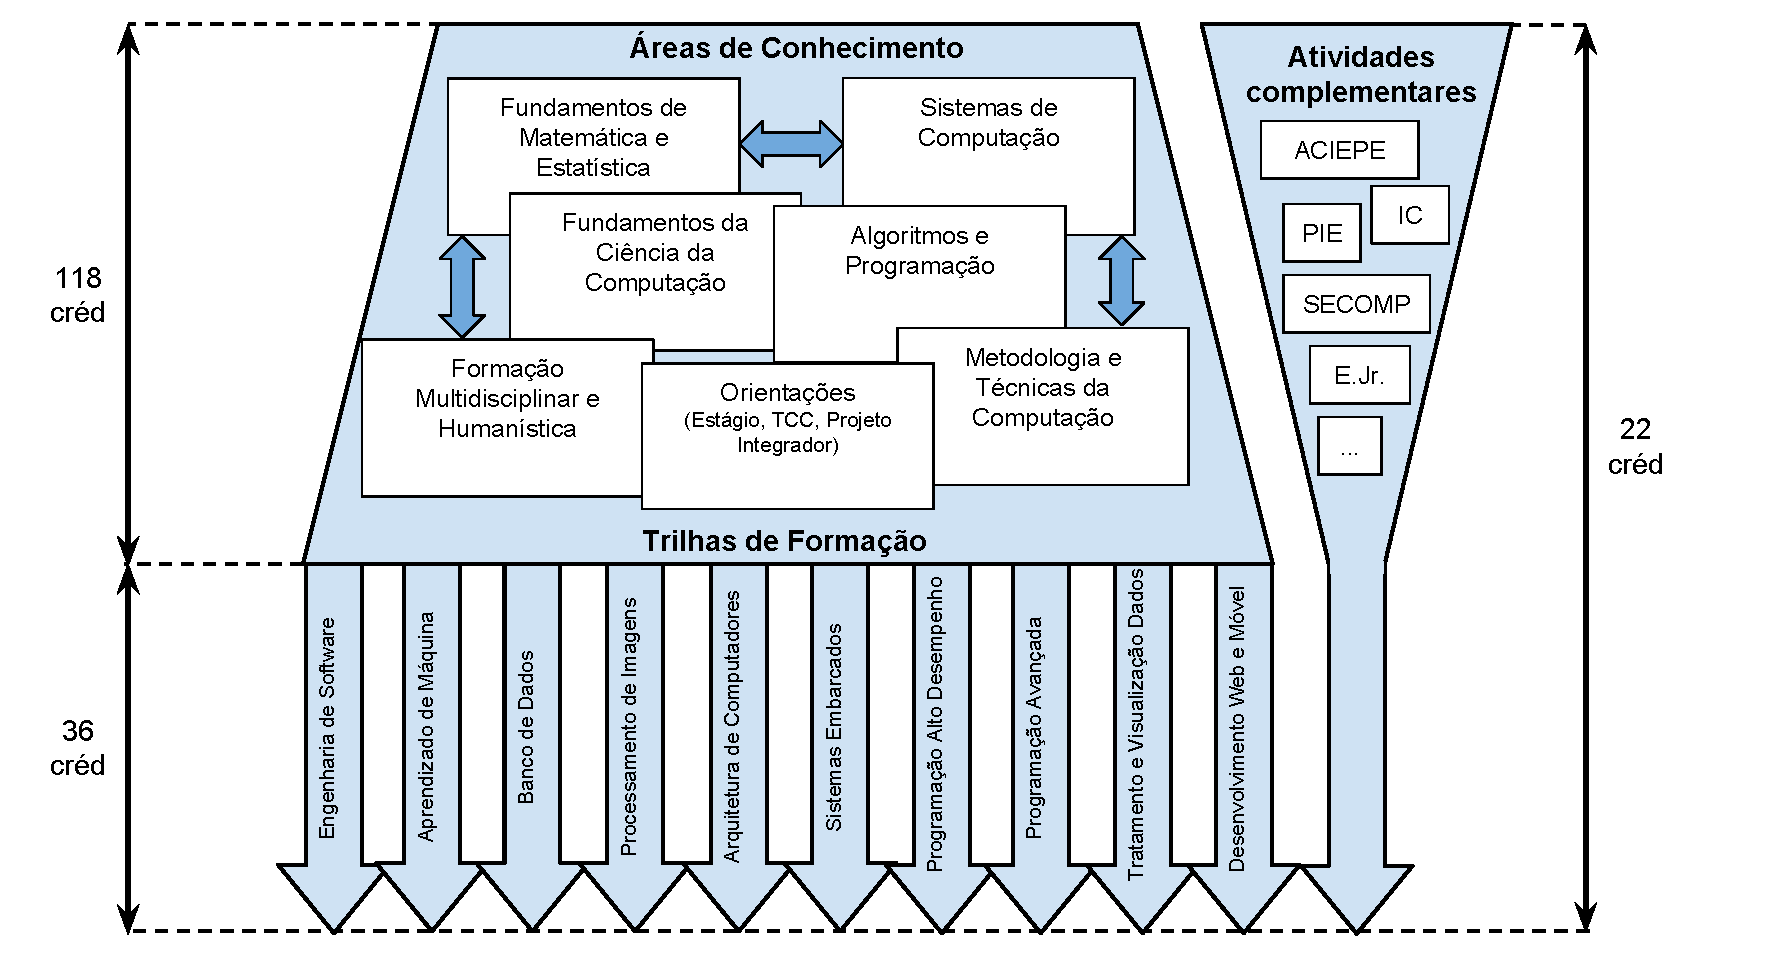
\includegraphics[width=\columnwidth]{bcc/imagens/perfil_egresso.pdf}
    \caption{Representação gráfica do perfil do egresso do curso de Ciência da Computação}
    \label{fig:perfil_egresso}
\end{figure}
\chapter{Marco Estrutural do Curso}~\label{sec:marco_estrutural}

Este capítulo apresenta detalhes da estrutura completa do Bacharelado em Ciência da Computação da Universidade Federal de São Carlos, campus São Carlos. Inclui visão geral dos tipos de atividades curriculares existentes, detalhes de integralização curricular, apresentação dos Núcleos de Conhecimento do curso, das Linhas de Formação e a matriz curricular e demais aspectos relacionados. 

\section{Visão Geral dos Tipos de Atividades Curriculares}

O marco estrutural do Bacharelado em Ciência da Computação da UFSCar, campus de São Carlos, é constituído pelos seguintes tipos de componentes curriculares: \textit{disciplinas obrigatórias}; \textit{disciplinas optativas profissionalizantes}; \textit{disciplinas optativas de humanas e complementares};
\textit{disciplinas eletivas};
\textit{atividades complementares}; \textit{trabalho de conclusão de curso} e \textit{estágio}. 


As disciplinas obrigatórias visam  desenvolver competências e habilidades que são essenciais na formação de um bacharel em ciência da computação. Essas disciplinas visam atender às diretrizes curriculares nacionais determinadas pelo ministério da educação~\cite{DCN-BCC}. 

As disciplinas optativas profissionalizantes fornecem aprofundamento em determinadas áreas da computação e também colaboram para tornar o curso mais flexível, permitindo que os estudantes possam adaptar o curso a demandas específicas, sejam elas pessoais, da academia, ou de mercado. 

O oferecimetno de um conjunto significativo de disciplinas optativas profissionalizantes foi um dos norteadores desta reformulação curricular. Assim, uma parcela significativa da carga horária em disciplinas que é exigida para a integralização curricular pode ser adaptada pelo próprio estudante. Nesta reformulação, aproximadamente 50\% da carga horária em disciplinas é composta por disciplinas optativas.

As disciplinas optativas de humanas e complementares, fornecem ao estudante formação humanística, cobrindo aspectos étnico-raciais, educação ambiental e linguagem brasileira de sinais (libras), que é uma exigência da legislação nacional ~\cite{Regimento-Geral-CursosGraduacao-UFSCar}. 

As disciplinas eletivas são quaisquer disciplinas oferecidas pelos cursos da UFSCar. Assim, o estudante pode escolher livremente por disciplinas que sejam oferecidas por qualuqer departamento desta universidade.

Essa estrutura curricular mais flexível, em que uma parte importante da formação do estudante se dá por meio  da sua escolha dentre um conjunto de disciplinas optativas, traz diversos benefícios. Com essa flexibilidade, busca-se não apenas uma estrutura que possa ser facilmente ajustável ao progresso do conhecimento científico e tecnológico, mas também que reforce o senso de responsabilidade e envolvimento do estudante, já que este passa a ser ator central da sua própria formação.

O Estágio neste curso de Ciência da Computação é uma atividade diferenciada, que é desenvolvida pelo estudante dentro de um ambiente real de trabalho (empresas) e que é supervisionada por um docente do curso que atua como "orientador", e por um supervisor dentro da empresa. O Estágio é realizado no último semestre do curso e seu objetivo é preparar o estudante para o exercício profissional.

O Trabalho de Conclusão de Curso (TCC) é um componente curricular que constitui-se de um trabalho acadêmico sobre um determinado tema relacionado ao Bacharelado em Ciência da Computação. O TCC é desenvolvido sob a supervisão de um docente e formalizado como uma monografia. O objeivo é expor o estudante a temas recentes e que extrapolam os limites dos conteúdos transmitidos durante o curso. Neste curso, o estudante tem a liberdade de optar pela realização do TCC ou pela realização do Estágio Obrigatório na finalização de seu curso, isto é, nao é obrigatória a realização dos dois. Também vale ressaltar que o TCC pode ser substituído pela realização de um ano de Iniciação Científica. Mais detalhes podem ser obtidos na Seção que descreve o Trabalho de Conclusão de Curso. 

As Atividades Complementares são atividades curriculares que não estão compreendidas no desenvolvimento regular das disciplinas do curso. São atividades de caráter acadêmico, científico, social e cultural realizadas pelo estudante ao longo de seu curso de graduação, que contribuem para o enriquecimento científico, profissional e cultural e para o desenvolvimento de valores e hábitos de colaboração e de trabalho em equipe. Este curso de Ciência da Computação prevê uma lista extensa e muitas oportunidades de atividades complementares que são oferecidas para os estudantes, como por exemplo, i) o desenvolvimento de projetos integradores; ii) iniciações científicas para engajamento do estudante em atividades de pesquisa; iii) oportunidades de atuar como monitores em disciplinas, etc. 

Para cada um dos tipos de atividades curriculares apresentados anteriomente é exigido um determinado número de créditos para integralização, como pode ser visto na Tabela~\ref{table: quadro_integraliza}. Note-se que o curso todo exige o cumprimento de 216 créditos, correspondendo a 3.240 horas em atividades curriculares, o que atende às diretrizes curriculares nacionais \cite{DCN-BCC}. As disciplinas optativas profissionalizantes são também chamadas de \textit{Optativas de Linha}, porque fazem parte de uma proposta inovadora deste curso de Ciência da Computação. Isso é detalhado mais adiante.   

\begin{table}
\caption{Quadro de Integraliza\c c\~ao Curricular}
\centering
\label{table: quadro_integraliza}
%\footnotesize
\begin{tabular}{|c|c|}
\hline
\hline
\textbf{Tipo de Atividade Curricular}  & \textbf{Quantidade de Créditos} \\
 & \textbf{Exigidos}\\
 & (1 crédito = 15 horas) \\

\hline
Disciplinas Obrigat\'orias & 118 Cr\'editos \\
\hline
Disciplinas Optativas Profissionalizantes (Optativas de Linha) & 36 Cr\'editos \\
\hline
Disciplinas Optativas de Humanas e Complementares & 4 Cr\'editos \\
\hline
Disciplinas Eletivas (quaisquer do campus) & 12 Cr\'editos \\
\hline
Estágio ou TCC (Trabalho de Conclusão do Curso) & 24 Cr\'editos \\
\hline
Atividades Complementares& 22 Cr\'editos \\
\hline
\hline
\textbf{Total de Cr\'editos para Integraliza\c c\~ao} & \textbf{216 Cr\'editos} \\
\hline
\textbf{Total de Horas para Integraliza\c c\~ao}  & \textbf{3.240 Horas} \\

\hline

\hline
\end{tabular}
\end{table}


\section{Núcleos de Conhecimento do Curso} \label{sec:marco_estrutural_areas_conhecimento}

O curso é organizado em Núcleos de Conhecimento para facilitar seu gerenciamento e fornecer uma visão mais macro da estrutura curricular. Cada núcleo de conhecimento engloba um conjunto de disciplinas relacionadas. Essa divisão facilita a administração do curso para manutenção de sua excelência, pois existe a figura do coordenador de núcleo, que é um professor do curso especialista nas disciplinas de um determinado núcleo , podendo reger adequadamente os conteúdos administrados nessas disciplinas. 

Para este curso foram definidos sete Núcleos de Conhecimento: (1) Fundamentos de Matemática e Estatística, (2) Fundamentos de Ciência da Computação, (3) Algoritmos e Programação, (4) Metodologia e Técnicas da Computação, (5) Sistemas de Computação, (6) Formação Multidisciplinar e Humanística e (7) Orientações. 

No Núcleo de Fundamentos de Matemática e Estatística encontram-se disciplinas como Cálculo Diferencial e Integral, Geometria Analítica, Álgebra Linear e Probabilidade e Estatística.

No Núcleo de Fundamentos de Ciência da Computação encontram-se disciplinas comológica matemática, teoria da computação, compiladores e paradigmas de linguagens de programação. Esse núcleo capacita o estudante em aspectos teóricos essenciais à ciência da computação, e que fornecem um embasamento mais profundo em relação aos cursos voltados especificamente à programação de computadores. 

O Núcleo de Algoritmos e Programação tem como foco o ensino do desenvolvimento de algoritmos e programas de computador, essencial para qualquer atividade ligada à computação. Esse núcleo visa desenvolver habilidades e competências relacionadas à construção de sistemas computacionais como atividade fim ou atividade meio. O objetivo das disciplinas deste núcleo de conhecimento é capacitar o estudante na programação de computadores e na resolução de problemas computacionais, fornecendo a ele as técnicas necessárias para o aproveitamento pleno das demais disciplinas do curso que tratam da computação. Exemplos de disciplinas desse núcleo são: Algoritmos e Estrutura de Dados, Programação Orientada a Objetos e Projeto e Análise de Algoritmos. 

O Núcleo de Metodologias e Técnicas da Computação traz uma série de tecnologias e metodologias computacionais como Engenharia de Software, Inteligência Artificial, Interação Humano-Computador e Banco de Dados. Esse núcleo visa desenvolver habilidades e competências relacionadas ao projeto e ao desenvolvimento de software.

O Núcleo de Sistemas de Computação apresentam soluções que são, em sua maioria, base para o funcionamento de software de mais alto nível, como sistemas operacionais, arquitetura e redes de computadores. Este Núcleo de Conhecimento trata de uma série de tópicos relacionados à construção de sistemas de computação, incluindo aspectos de hardware e software. 

O Núcleo de Formação Multidisciplinar e Humanística complementa a formação do estudante por meio de disciplinas do núcleo de ciências humanas e disciplinas eletivas. Esse núcleo visa desenvolver habilidades e valores relacionados à atuação do egresso na sociedade com o intuito de formar um profissional consciente de seu papel ético, humano e social. Também tem como objetivo permitir que o estudante diversifique e complemente sua formação. 

No Núcleo de Orientações os estudantes também são envolvidos em atividades que demandam supervisão de docentes. Nesse conjunto destacam-se as Iniciações Científicas, o Trabalho de Conclusão de Curso, o Estágio e o Projeto Integrador. O objetivo desse núcleo é desenvolver habilidades e competências tanto de atuação do estudante no mercado de trabalho quanto seu desenvolvimento para atuação científica em pesquisas relacionadas com computação. 

%A lista de possíveis disciplinas optativas a serem oferecidas \helena{(incompleta)}{} é apresentada na Figura~\ref{fig:eixo_optativas}.

%\begin{figure}[H]
%\centering
%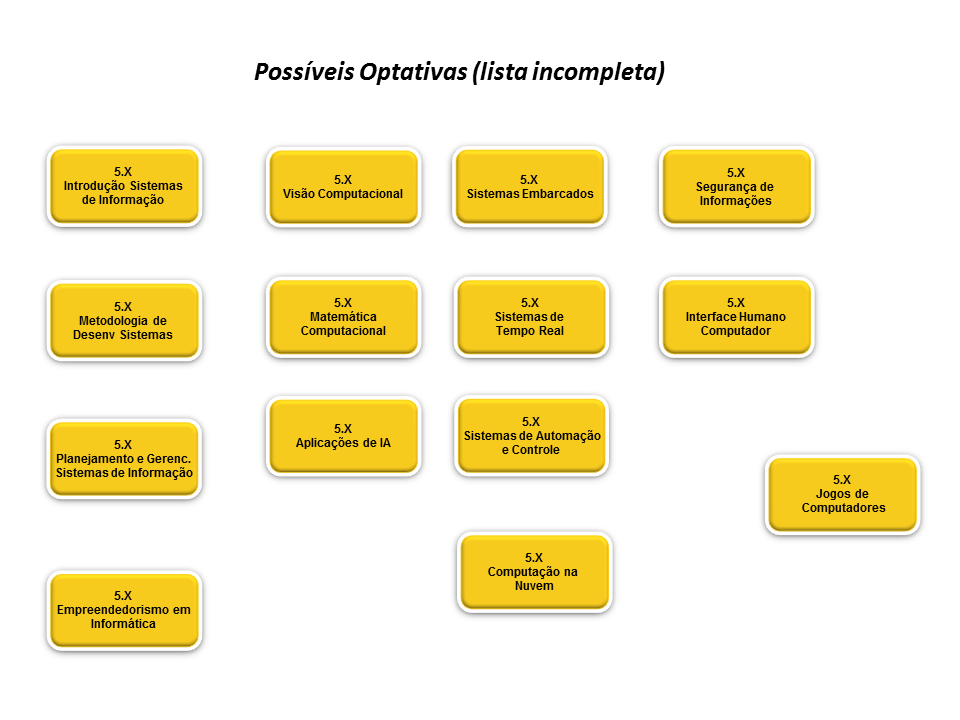
\includegraphics[width=0.8\textwidth]{imagens/eixo_optativas.png}
%\caption{Possíveis Disciplinas Optativas \helenacomentario{REFAZER}}
%\label{fig:eixo_optativas}
%\end{figure}



%\begin{figure}[htb!]
%\centering
%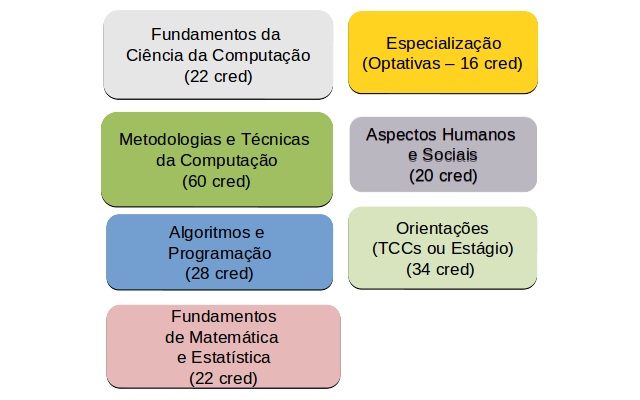
\includegraphics[width=\textwidth]{imagens/eixos2.png}
%caption{Eixos de formação do curso.}
%\label{fig:eixos}
%\end{figure}


\section{Matriz Curricular}

A matriz curricular completa é apresentada na Figura~\ref{fig:matriz}. As linhas da tabela referem-se aos oito semestres do curso (de S1 a S8), indicados pelos S\# do lado esquerdo da figura. As colunas delimitam os sete núcleos de conhecimento citadas anteriormente. Note-se que também há na parte inferior da matriz curricular o núcleo de orientações, incluindo o Estágio e o Trabalho de Conclusão de Curso. Cada núcleo de conhecimento também é destacado por uma cor específica. 

As caixas com bordas cheias representam as disciplinas obrigatórias, isto é, aquelas que todo estudante deve cursar. As caixas com bordas arredondadas são disciplinas optativas que podem ser escolhidas pelo estudante para configurar seu curso. Dentro de cada caixa observa-se embaixo da sigla da disciplina uma numeração no formato \#:\#/\#. Essa numeração indica o número de créditos total da disciplina, dividido em créditos teóricos e práticos (em laboratório). Por exemplo, a disciplina Construção de Algoritmos e Programação (CAP) possui 8 créditos, sendo 4 teóricos e 4 práticos. 

Nesta figura pode-se visualizar também o número de disciplinas por semestre e também a carga em créditos de cada semestre. Por exemplo, no primeiro semestre do curso (S1) há quatro disciplinas obrigatórias que precisam ser cursadas pelo estudante e isso contabiliza 22 créditos. O número de créditos de cada semestre pode ser visto embaixo da sigla S\# que indica o número do semestre.

As disciplinas optativas profissionalizantes (caixas com bordas pontilhadas) permitem que o estudante possa configurar seu curso e elas começam a partir do quinto semestre. Por exemplo, no semestre 5 (S5), espera-se que o estudante curse 24 créditos em disciplinas, como pode ser visto pelo número embaixo da sigla S\#. Entretanto, nesse semestre há duas disciplinas obrigatórias (Cálculo Numérico e PAA) que somam 8 créditos e que obrigatoriamente devem ser cursadas pelo estudante, restando 16 créditos para serem feitos. Esses 16 créditos restantes que devem ser feitos (equivalente a 4 disciplinas de 4 créditos) podem ser livremente escolhido pelo estudante para configurar seu semestre. Como pode ser observado, há 7 disciplinas optativas oferecidas neste semestre, assim, dessas 7, o estudante tem a liberdade de optar por 4, contabilizando os 24 créditos exibidos do semestre. 


\subsection{O Conceito de Linhas de Formação}

Outro aspecto importante desta reformulação curricular é o conceito de "Linhas de Formação", que só é possível graças à quantidade de disciplinas optativas oferecidas. Uma Linha de Formação é um agrupamento sequencial de 2 ou 3 disciplinas relacionadas e que fornecem ao estudante um aprofundamento em núcleos específicos da computação. O estudante tem a opção de iniciar as linhas a partir do quinto semestre, visto que antes disso há apenas disciplinas obrigatórias. As Linhas de Formação são opcionais, isto é, o estudante pode optar por não fazer linhas e seguir para uma formação mais generalista.  

O curso oferece 10 Linhas de Formação, que são mostradas abaixo com suas respectivas disciplinas:

\begin{enumerate}
\item \textbf{Engenharia de Software}. Composta pelas disciplinas: Engenharia de Software 2, Arquitetura de Software e Padrões e DevOps;
\item \textbf{Aprendizado de Máquina}. Composta pelas disciplinas: Aprendizado de Máquina 1 e Aprendizado de Máquina 2;
\item \textbf{Banco de Dados}. Composta pelas disciplinas: Projeto e Implementação de Banco de Dados e Banco de Dados para Ciência de Dados;
\item \textbf{Processamento Digital de Imagens e Visão Computacional}. Composta pelas disciplinas: Processamento Digital de Imagens, Processamento Digital de Imagens 3D e Vídeos e Visão Computacional;
\item \textbf{Arquitetura de Computadores}. Composta pelas disciplinas: Sistemas Digitais e Arquiteturas de Alto Desempenho; 
\item \textbf{Tratamento e Visualização de Dados}. Composta pelas disciplinas: Computação Gráfia e Processamento e Visualização de Dados;
\item \textbf{Sistemas Embarcados}. Composta pelas disciplinas: Engenharia de Sistemas, Arquitetura e Organização de Computadores 2 e Projeto de Sistemas Computacionais Embarcados; 
\item \textbf{Programação de Alto Desempenho}. Composta pelas disciplinas: Sistemas Distribuídos, Programação Paralela e Distribuída e Processamento de Dados em Escala;
\item \textbf{Programação Avançada}. Composta pelas disciplinas: Programação Orientada a Objetos Avançada e Paradigmas de Linguagens de Programação;
\item \textbf{Desenvolvimento Web e Móvel}. Composta pelas disciplinas: Desenvolvimento de Software para Web 1, Desenvolvimento de Software para Web 2 e Desenvolvimento Móvel.
\end{enumerate}

Como pode ser observado na Figura~\ref{fig:matriz}, as disciplinas optativas profissionalizantes começam no semestre 5 e é a partir desse semestre que o estudante pode iniciar determinadas linhas de formação. Por exemplo, ao seguir para o quinto semestre, o estudante poderia optar por seguir as seguintes quatro Linhas de Formação: Engenharia de Software, Aprendizado de Máquina, Programação Avançada e Desenvovimetno Web e Móvel. Dessa forma, o estudante precisaria optar por cursar as disciplinas de Engenharia de Software 2 (ES2), Aprendizado de Máquina 1 (AM1), Programação Orientada a Objetos Avançada (POO Avançada) e Desenvolvimento de Software para Web 1 (Des Softw Web 1), pois essas são as primeiras disciplinas de cada uma das quatro linhas escolhidas. No semestre seguinte, sexto semestre, o estudante poderia ainda optar por continuar ou não nessas linhas. Caso ele opte por continuar, ele deve então escolher as disciplinas que sequenciam essas anteriores. 

\newpage
\begin{figure}[H]
\centering
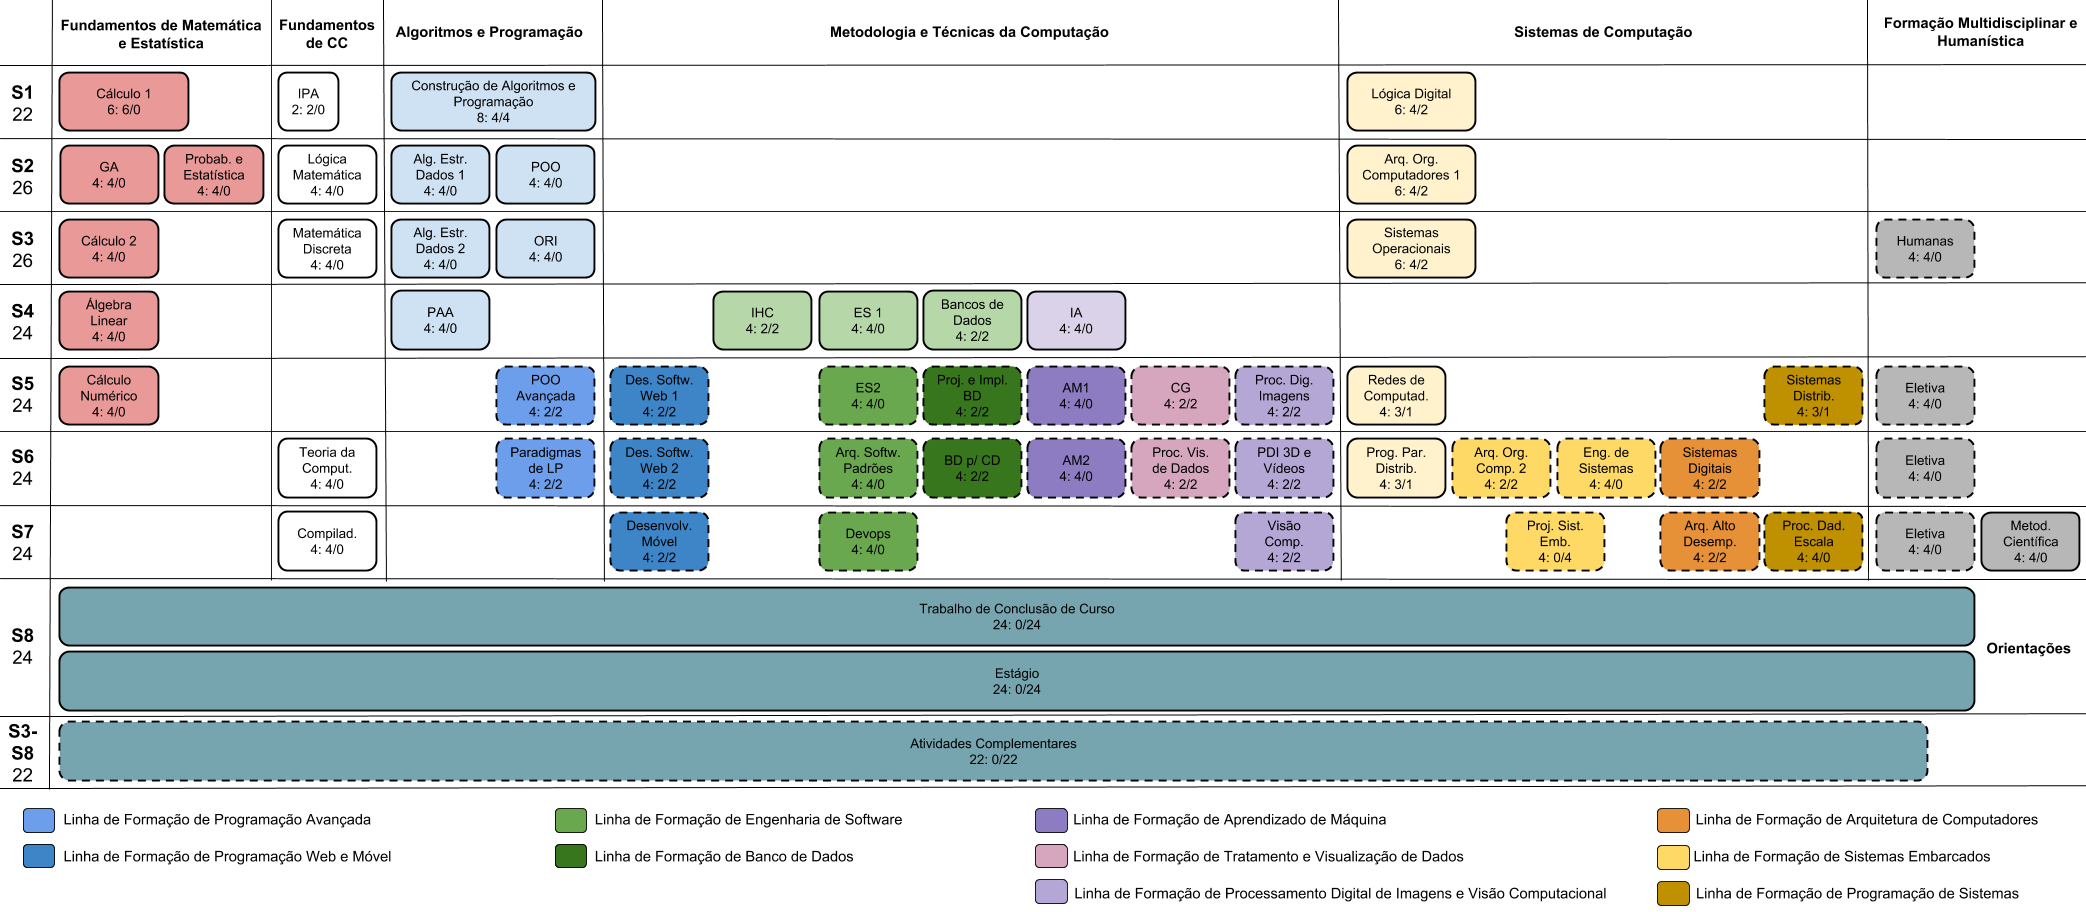
\includegraphics[angle=90,width=0.63\textwidth]{imagens/Grade.png}
\caption{Matriz curricular completa}
\label{fig:matriz}
\end{figure}

A Figura~\ref{fig:matriz_visao_aluno} apresenta uma visão diferente da matriz curricular apresentada na Figura~\ref{fig:matriz}, pois ela apresenta a visão do estudante, ou seja, as disciplinas obrigatórias e a quantidade de optativas de linha (profissionalizantes) que devem ser cursadas. Nessa visão, fica claro que o estudante deve cursar 9 disciplinas optativas de linha, escolhendo a partir das várias opções disponíveis mostradas na Figura~\ref{fig:matriz}.


\begin{figure}[H]
\centering
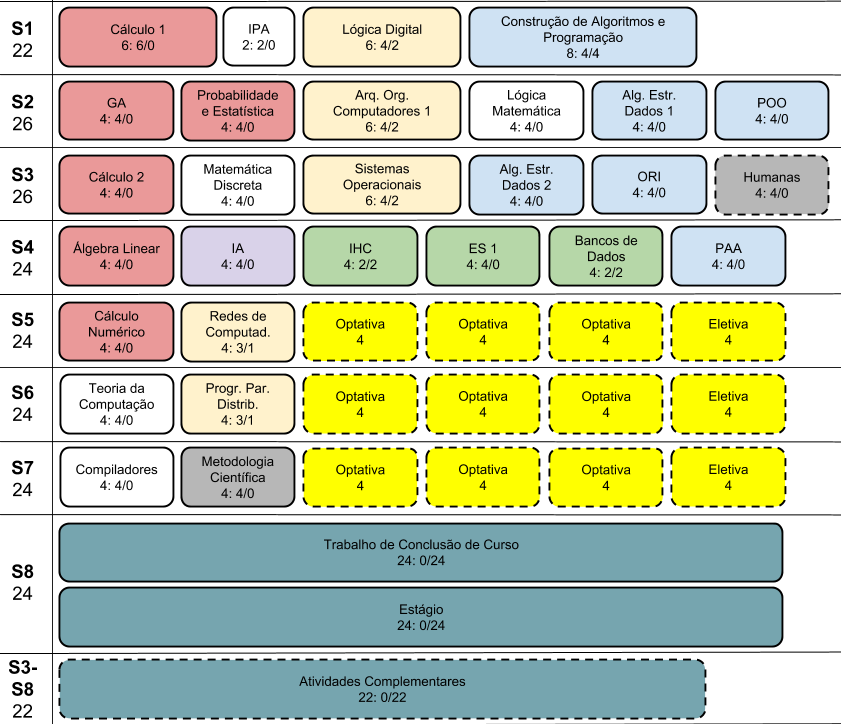
\includegraphics[width=1\textwidth]{imagens/Grade_visao_aluno.png}
\caption{Matriz curricular completa na visão do estudante}
\label{fig:matriz_visao_aluno}
\end{figure}


\subsection{Detalhamento da Matriz Curricular}

Esta seção apresenta o detalhamento da matriz curricular, destacando, para cada semestre do curso, as disciplinas, a sigla que as representa, o caráter (Obrigatória, Optativa ou Eletiva), os pré-requisitos, os departamentos ofertantes e o número de  créditos de cada uma. Esse detalhamento é apresentado da Tabela ~\ref{tab:matriz1} até a Tabela~\ref{tab:matriz8}.

%\pagebreak

\singlespacing

%%%%%%%%%%%%%%%%%%
%% Semestre 1: %%%
%%%%%%%%%%%%%%%%%%

\begin{table}[H]
\caption{Semestre 1}
\centering
\footnotesize
\begin{tabular}{|c|c|c|c|c|c|c|c|} %c|}
\hline
\hline
\multicolumn{5}{|c|}{\textbf{Semestre 1}}  &  \multicolumn{3}{|c|}{\textbf{Créditos}} \\
\hline
\hline
\textbf{Disciplina} & \textbf{Sigla} & \textbf{Caráter} & \textbf{Pré-} & \textbf{Depto} &  \textbf{T}  &  \textbf{P}  & \textbf{Total} \\ 
& & & \textbf{Requisitos}  & \textbf{Ofertante} & & & \\
\hline 
Cálculo Diferencial & Cálculo 1 & Obrig & -- & DM  & 6 & 0 & 6 \\
e Integral 1 (82210)& & & & & & & \\
\hline
Introdução ao Pensamento & IPA & Obrig & -- & DC  & 2 & 0 & 2 \\
Algorítmico & & & & & & & \\
\hline
Construção de Algoritmos & CAP & Obrig & -- & DC  & 4 & 4 & 8 \\
e Programação & & & & & & & \\
\hline
Lógica Digital & LD & Obrig & -- & DC & 4 & 2 & 6 \\
\hline
\hline
\multicolumn{5}{|r|}{\textbf{Total:}}  &  \textbf{16}  &  \textbf{6}   & \textbf{22} \\ %& \textbf{16}  \\
\hline
\hline
\end{tabular}
\label{tab:matriz1}
\end{table}


%%%%%%%%%%%%%%%%%%
%% Semestre 2: %%%
%%%%%%%%%%%%%%%%%%

\begin{table}[H]
\caption{Semestre 2}
\centering
\footnotesize
\begin{tabular}{|c|c|c|c|c|c|c|c|} %c|}
\hline
\hline
\multicolumn{5}{|c|}{\textbf{Semestre 2}}  &  \multicolumn{3}{|c|}{\textbf{Créditos}} \\
\hline
\hline
\textbf{Disciplina} & \textbf{Sigla} & \textbf{Caráter} & \textbf{Pré-} & \textbf{Depto} &  \textbf{T}  &  \textbf{P}  & \textbf{Total} \\ 
& & & \textbf{Requisitos}  & \textbf{Ofertante} & & & \\
\hline 
Geometria Analítica (81116) & GA & Obrig & -- & DM & 4 & 0 & 4 \\
\hline
Lógica Matemática & LM & Obrig & -- & DC & 4 & 0 & 4 \\
\hline
Algoritmos e Estruturas & AED1 & Obrig & CAP & DC  & 4 & 0 & 4 \\
de Dados 1 & & & & & & & \\
\hline
Programação Orientada & POO & Obrig & CAP & DC  & 2 & 2 & 4 \\
a Objetos & & & & & & & \\
\hline
Arquitetura e Organização & Arq1 & Obrig & LD & DC & 4 & 2 & 6 \\
de Computadores 1 & & & & & & & \\
\hline
Probabilidade e Estatística (150010) & ProbEst & Obrig & -- & DES & 4 & 0 & 4 \\
%de Texto & & & & & & & \\
\hline
\hline
\multicolumn{5}{|r|}{\textbf{Total:}}  &  \textbf{22}  &  \textbf{4}   & \textbf{26} \\ %& \textbf{16}  \\
\hline
\hline
\end{tabular}
\label{tab:matriz2}
\end{table}


%%%%%%%%%%%%%%%%%%
%% Semestre 3: %%%
%%%%%%%%%%%%%%%%%%

\begin{table}[H]
\caption{Semestre 3}
\centering
\footnotesize
\begin{tabular}{|c|c|c|c|c|c|c|c|} %c|}
\hline
\hline
\multicolumn{5}{|c|}{\textbf{Semestre 3}}  &  \multicolumn{3}{|c|}{\textbf{Créditos}} \\
\hline
\hline
\textbf{Disciplina} & \textbf{Sigla} & \textbf{Caráter} & \textbf{Pré-} & \textbf{Depto} &  \textbf{T}  &  \textbf{P}  & \textbf{Total} \\ 
& & & \textbf{Requisitos}  & \textbf{Ofertante} & & & \\
\hline 
Cálculo Diferencial & CDS & Obrig & Cálculo 1 & DM  & 4 & 0 & 4 \\
e Séries (82260) & & & & & & & \\
\hline
Matemática Discreta & MD & Obrig & -- & DC  & 4 & 0 & 4 \\
\hline
Algoritmos e Estruturas & AED2 & Obrig & AED1 & DC  & 4 & 0 & 4 \\
de Dados 2 & & & & & & & \\
\hline
Organização e Recuperação & ORI & Obrig & AED1 & DC  & 4 & 0 & 4 \\
da Informação & & & & & & & \\
\hline
Sistemas Operacionais & SO & Obrig & Arq1 & DC  & 4 & 2 & 6 \\
\hline
Optativa de Humanas & -- & Opt & -- & DCSo/DL & 4 & 0 & 4 \\
e Complementares & & & & /DCI/DFMC & & & \\
Escolher uma da Tabela \ref{tab:optativas-humanas-complementares} & & & & & & & \\
\hline

\hline
\hline
\multicolumn{5}{|r|}{\textbf{Total:}}  &  \textbf{24}  &  \textbf{2}   & \textbf{26} \\ %& \textbf{16}  \\
\hline
\hline
\end{tabular}
\label{tab:matriz3}
\end{table}


%%%%%%%%%%%%%%%%%%
%% Semestre 4: %%%
%%%%%%%%%%%%%%%%%%

\begin{table}[H]
\caption{Semestre 4}
\centering
\footnotesize
\begin{tabular}{|c|c|c|c|c|c|c|c|} %c|}
\hline
\hline
\multicolumn{5}{|c|}{\textbf{Semestre 4}}  &  \multicolumn{3}{|c|}{\textbf{Créditos}} \\
\hline
\hline
\textbf{Disciplina} & \textbf{Sigla} & \textbf{Caráter} & \textbf{Pré-} & \textbf{Depto} &  \textbf{T}  &  \textbf{P}  & \textbf{Total} \\ 
& & & \textbf{Requisitos}  & \textbf{Ofertante} & & & \\
\hline 
Álgebra Linear (80136) & AlgeLin & Obrig & GA & DM  & 4 & 0 & 4 \\
\hline

Interação Humano- & IHC & Obrig & CAP & DC & 2 & 2 & 4 \\
Computador & & & & & & & \\

\hline
Projeto e Análise de & PAA & Obrig & AED1 & DC  & 4 & 0 & 4 \\
Algoritmos & & & & & & & \\
\hline
Engenharia de  & ES1 & Obrig & POO & DC  & 4 & 0 & 4 \\
Software 1 & & & & & & & \\
\hline
Banco de Dados & BD & Obrig & AED1 & DC  & 2 & 2 & 4 \\
\hline
Inteligência Artificial & IA & Obrig & AED1 & DC & 2 & 2 & 4 \\
\hline

\hline
\hline
\multicolumn{5}{|r|}{\textbf{Total:}}  &  \textbf{18}  &  \textbf{6}   & \textbf{24} \\ %& \textbf{16}  \\
\hline
\hline
\end{tabular}
\label{tab:matriz4}
\end{table}



%%%%%%%%%%%%%%%%%%
%% Semestre 5: %%%
%%%%%%%%%%%%%%%%%%


\begin{table}[H]
\caption{Semestre 5}
\centering
\footnotesize
\begin{tabular}{|c|c|c|c|c|c|c|c|} %c|}
\hline
\hline
\multicolumn{5}{|c|}{\textbf{Semestre 5}}  &  \multicolumn{3}{|c|}{\textbf{Créditos}} \\
\hline
\hline
\textbf{Disciplina} & \textbf{Sigla} & \textbf{Caráter} & \textbf{Pré-} & \textbf{Depto} &  \textbf{T}  &  \textbf{P}  & \textbf{Total} \\ 
& & & \textbf{Requisitos}  & \textbf{Ofertante} & & & \\
\hline 

Cálculo Numérico (83020) & Cáculo & Obrig & Cálculo 1 & DM & 4 & 0 & 4 \\
& Numérico & & GA & & & & \\
\hline

Redes de Computadores & Redes & Obrig & SO & DC & 4 & 0 & 4 \\
\hline

Optativa & --  & Opt & Depende & DC  & 4 & 0 & 4 \\
Profissionalizante & & & da Escolha & & & & \\
(\textit{Optativa de Linha}) & & & & & & & \\
Tabela~\ref{tab:OptTrilha-Semestre5} & & & & & & & \\
\hline

Optativa & --  & Opt & Depende & DC  & 4 & 0 & 4 \\
Profissionalizante & & & da Escolha & & & & \\
(\textit{Optativa de Trilha}) & & & & & & & \\
Tabela~\ref{tab:OptTrilha-Semestre5} & & & & & & & \\
\hline


Optativa & --  & Opt & Depende & DC  & 4 & 0 & 4 \\
Profissionalizante & & & da Escolha & & & & \\
(\textit{Optativa de Linha}) & & & & & & & \\
Tabela~\ref{tab:OptTrilha-Semestre5} & & & & & & & \\
\hline

Eletiva  & --  & Eletiva & -- & Qualquer & 4 & 0 & 4 \\
(\textit{Qualquer Disciplina} & & & & & & & \\
\textit{do Campus}) & & & & & & & \\
\hline




\hline


\hline
\hline
\multicolumn{5}{|r|}{\textbf{Total:}}  &  \textbf{24}  &  \textbf{0}   & \textbf{24} \\ %& \textbf{16}  \\
\hline
\hline
\end{tabular}
\label{tab:matriz5}
\end{table}



%%%%%%%%%%%%%%%%%%
%% Semestre 6: %%%
%%%%%%%%%%%%%%%%%%

\begin{table}[H]
\caption{Semestre 6}
\centering
\footnotesize
\begin{tabular}{|c|c|c|c|c|c|c|c|} %c|}
\hline
\hline
\multicolumn{5}{|c|}{\textbf{Semestre 6}}  &  \multicolumn{3}{|c|}{\textbf{Créditos}} \\
\hline
\hline
\textbf{Disciplina} & \textbf{Sigla} & \textbf{Caráter} & \textbf{Pré-} & \textbf{Depto} &  \textbf{T}  &  \textbf{P}  & \textbf{Total} \\ 
& & & \textbf{Requisitos}  & \textbf{Ofertante} & & & \\
\hline 
Teoria da Computação & TC & Obrig & MD & DC & 4 & 0 & 4 \\
\hline

Programação Paralela & PPD & Obrig & SO & DC & 2 & 2 & 4 \\
e Distribuída & & & & & & & \\
\hline


Optativa & --  & Opt & Depende & DC  & 4 & 0 & 4 \\
Profissionalizante & & & da Escolha & & & & \\
(\textit{Optativa de Linha}) & & & & & & & \\
Tabela~\ref{tab:OptTrilha-Semestre6} & & & & & & & \\
\hline

Optativa & --  & Opt & Depende & DC  & 4 & 0 & 4 \\
Profissionalizante & & & da Escolha & & & & \\
Tabela~\ref{tab:OptTrilha-Semestre6} & & & & & & & \\
\hline


Optativa & --  & Opt & Depende & DC  & 4 & 0 & 4 \\
Profissionalizante & & & da Escolha & & & & \\
(\textit{Optativa de Linha}) & & & & & & & \\
Tabela~\ref{tab:OptTrilha-Semestre6} & & & & & & & \\
\hline

Eletiva  & --  & Eletiva & -- & Qualquer & 4 & 0 & 4 \\
(\textit{Qualquer Disciplina} & & & & & & & \\
\textit{do Campus}) & & & & & & & \\
\hline




\hline


\hline
\hline
\multicolumn{5}{|r|}{\textbf{Total:}}  &  \textbf{22}  &  \textbf{2}   & \textbf{24} \\ %& \textbf{16}  \\
\hline
\hline
\end{tabular}
\label{tab:matriz6}
\end{table}


%%%%%%%%%%%%%%%%%%
%% Semestre 7: %%%
%%%%%%%%%%%%%%%%%%

\begin{table}[H]
\caption{Semestre 7}
\centering
\footnotesize
\begin{tabular}{|c|c|c|c|c|c|c|c|} %c|}
\hline
\hline
\multicolumn{5}{|c|}{\textbf{Semestre 7}}  &  \multicolumn{3}{|c|}{\textbf{Créditos}} \\
\hline
\hline
\textbf{Disciplina} & \textbf{Sigla} & \textbf{Caráter} & \textbf{Pré-} & \textbf{Depto} &  \textbf{T}  &  \textbf{P}  & \textbf{Total} \\ 
& & & \textbf{Requisitos}  & \textbf{Ofertante} & & & \\
\hline 

Construção & Compiladores & Obrig & TC, CAP & DC & 4 & 0 & 4 \\
de Compiladores & & & & & & &  \\

\hline

Metodologia & MC & Obrig & -- & DC & 4 & 0 & 4 \\
Científica & & & & & & &  \\
\hline

Optativa & --  & Opt & Depende & DC  & 4 & 0 & 4 \\
Profissionalizante & & & da Escolha & & & & \\
(\textit{Optativa de Linha}) & & & & & & & \\
Tabela~\ref{tab:OptTrilha-Semestre7} & & & & & & & \\
\hline

Optativa & --  & Opt & Depende & DC  & 4 & 0 & 4 \\
Profissionalizante & & & da Escolha & & & & \\
(\textit{Optativa de Trilha}) & & & & & & & \\
Tabela~\ref{tab:OptTrilha-Semestre7} & & & & & & & \\
\hline


Optativa & --  & Opt & Depende & DC  & 4 & 0 & 4 \\
Profissionalizante & & & da Escolha & & & & \\
(\textit{Optativa de Linha}) & & & & & & & \\
Tabela~\ref{tab:OptTrilha-Semestre7} & & & & & & & \\
\hline

Eletiva  & --  & Eletiva & -- & Qualquer & 4 & 0 & 4 \\
(\textit{Qualquer Disciplina} & & & & & & & \\
\textit{do Campus}) & & & & & & & \\
\hline




\hline


\hline
\hline
\multicolumn{5}{|r|}{\textbf{Total:}}  &  \textbf{24}  &  \textbf{0}   & \textbf{24} \\ %& \textbf{16}  \\
\hline
\hline
\end{tabular}
\label{tab:matriz7}
\end{table}


%%%%%%%%%%%%%%%%%%
%% Semestre 8: %%%
%%%%%%%%%%%%%%%%%%

\begin{table}[H]
\caption{Semestre 8}
\centering
\footnotesize
\begin{tabular}{|c|c|c|c|} %c|}
\hline
\hline
\multicolumn{1}{|c|}{\textbf{Semestre 8}}  &  \multicolumn{3}{|c|}{\textbf{Créditos}} \\
\hline
\hline
\textbf{Disciplina} &  \textbf{T}  &  \textbf{P}  & \textbf{Total} \\ 
\hline 

Estágio ou Trabalho de Conclusão de Curso & 0 & 24 & 24 \\

\hline

\hline

\textbf{Total:}  &  \textbf{0}  &  \textbf{24}   & \textbf{24} \\ 

\hline
\hline
\end{tabular}
\label{tab:matriz8}
\end{table}


%-----------------------------


\begin{table}[H]
\caption{Optativas de Linha do Semestre 5}
\centering
\footnotesize
\begin{tabular}{|c|c|c|c|c|c|c|c|} %c|}
\hline
\hline
\multicolumn{5}{|c|}{\textbf{Optativas de Linha do Semestre 5}}  &  \multicolumn{3}{|c|}{\textbf{Créditos}} \\
\hline
\hline
\textbf{Disciplina} & \textbf{Sigla} & \textbf{Caráter} & \textbf{Pré-} & \textbf{Depto} &  \textbf{T}  &  \textbf{P}  & \textbf{Total} \\ 
& & & \textbf{Requisitos}  & \textbf{Ofertante} & & & \\
\hline 
Programação Orientada a & POOA & Opt & POO, AED1 & DC & 2 & 2 & 4 \\
Objetos Avançada & & & & & & & \\ 
\hline
Desenvolvimento de Software & DSW 1 & Opt & BD & DC & 0 & 4 & 4 \\
para Web 1 & & & & & & & \\
\hline
Engenharia de Software 2 & ES2 & Opt & ES1 & DC & 4 & 0 & 4 \\
\hline
Projeto e Implementação & PIBD & Opt & BD & DC & 2 & 2 & 4 \\
de Banco de Dados & & & & & & & \\
\hline
Aprendizado de Máquina 1 & AM1 & Opt & IA, ProbEst & DC & 4 & 0 & 4 \\
\hline
Computação Gráfica & CG & Opt & GA, AED1 & DC & 4 & 0 & 4 \\
\hline
Processamento Digital & PDI & Opt & CAP, GA & DC & 2 & 2 & 4 \\
de Imagens & & & Cálculo 1 & & & & \\  
\hline
Sistemas Distribuídos & SD & Opt & SO & DC & 4 & 0 & 4 \\
\hline
\hline

\multicolumn{5}{|r|}{Escolher Três Disciplinas (12 créditos) desse Conjunto:}  &    &     &  \\
\hline
\hline
\end{tabular}
\label{tab:OptTrilha-Semestre5}
\end{table}


\begin{table}[H]
\caption{Optativas de Linha do Semestre 6}
\centering
\footnotesize
\begin{tabular}{|c|c|c|c|c|c|c|c|} %c|}
\hline
\hline
\multicolumn{5}{|c|}{\textbf{Optativas de Linha do Semestre 6}}  &  \multicolumn{3}{|c|}{\textbf{Créditos}} \\
\hline
\hline
\textbf{Disciplina} & \textbf{Sigla} & \textbf{Caráter} & \textbf{Pré-} & \textbf{Depto} &  \textbf{T}  &  \textbf{P}  & \textbf{Total} \\ 
& & & \textbf{Requisitos}  & \textbf{Ofertante} & & & \\
\hline 
Paradigmas de Linguagens & PLP & Opt & PAA & DC & 2 & 2 & 4 \\
de Programação & & & & & & & \\
\hline
Desenvolvimento de Software & DSW 2 & Opt & DSW 1 & DC & 0 & 4 & 4 \\
para Web 2 & & & & & & & \\
\hline
Arquitetura de Software & ASP & Opt & ES2 & DC & 4 & 0 & 4 \\
e Padrões & & & & & & &  \\
\hline
Banco de Dados para & BDCD & Opt & PIBD & DC & 2 & 2 & 4 \\
Ciência de Dados & & & & & & & \\
\hline
Aprendizado de Máquina 2 & AM2 & Opt & AM1 & DC & 4 & 0 & 4 \\
\hline
Processamento e Visualização & PVD & Opt & CG & DC & 2 & 2 & 4 \\
de Dados & & & & & & & \\
\hline
Processamento Digital de & PDI3D & Opt & PDI & DC & 2 & 2 & 4 \\
Imagens 3D e Vídeos & & & & & & & \\  
\hline
Arquitetura e Organização & Arq2 & Opt & Arq1 & DC & 2 & 2 & 4 \\
de Computadores 2 & & & & & & & \\
\hline
Engenharia de Sistemas & EngeSist & Opt & ES1 & DC & 4 & 0 & 4 \\
\hline
Sistemas Digitais & SistDig & Opt & LD & DC & 2 & 2 & 4 \\
\hline
\hline
\multicolumn{5}{|r|}{\textbf{Escolher Três Disciplinas (12 créditos) desse Conjunto: }} &    &     &  \\ %& \textbf{16}  \\
\hline
\hline
\end{tabular}
\label{tab:OptTrilha-Semestre6}
\end{table}





\begin{table}[H]
\caption{Optativas de Linha do Semestre 7}
\centering
\footnotesize
\begin{tabular}{|c|c|c|c|c|c|c|c|} %c|}
\hline
\hline
\multicolumn{5}{|c|}{\textbf{Optativas de Linha do Semestre 7}}  &  \multicolumn{3}{|c|}{\textbf{Créditos}} \\
\hline
\hline
\textbf{Disciplina} & \textbf{Sigla} & \textbf{Caráter} & \textbf{Pré-} & \textbf{Depto} &  \textbf{T}  &  \textbf{P}  & \textbf{Total} \\ 
& & & \textbf{Requisitos}  & \textbf{Ofertante} & & & \\
\hline 
Desenvolvimeto Móvel & DMovel & Opt & DSW 2 & DC & 0 & 4 & 4 \\
\hline
DevOps & DevOps & Opt & ES2 & DC & 0 & 4 & 4 \\
\hline
Visão Computacional & VC & Opt & (AlgeLin e PDI) & DC & 2 & 2 & 4 \\
& & & ou PSD & & & &  \\
\hline
Projeto de Sistemas & PDI3D & Opt & EngSist, Arq2  & DC & 0 & 4 & 4 \\
Computacionais Embarcados & & & & & & & \\  
\hline
Arquiteturas de Alto & Arq3 & Opt & Arq1 & DC & 2 & 2 & 4 \\
Desempenho & & & & & & & \\
\hline
Processamento de Dados & ProcDados & Opt & SO & DC & 2 & 2 & 4 \\
em Escala & & & & & & & \\
\hline
\hline
\multicolumn{5}{|r|}{\textbf{Escolher Três Disciplinas (12 créditos) desse Conjunto:}}  &    &     &  \\ %& \textbf{16}  \\
\hline
\hline
\end{tabular}
\label{tab:OptTrilha-Semestre7}
\end{table}


%-----------------------------------------










% --------------------------


\doublespacing

A Tabela~\ref{tab:optativas-humanas-complementares} mostra o conjunto de disciplinas optativas de humanas e complementares disponível. Como comentado anteriormente, no terceiro semestre o estudante deverá escolher uma disciplina desse conjunto. 


\singlespacing

%%%%%%%%%%%%%%%%%%%%%%%%%%%%%
%% Optativas de Humanas:  %%%
%%%%%%%%%%%%%%%%%%%%%%%%%%%%%

\begin{table}[H]
\caption{Optativas de Humanas e Complementares}
\centering
%\footnotesize
\begin{tabular}{|c|c|c|c|c|}
\hline
\hline
\multicolumn{2}{|c|}{\textbf{Disciplinas Optativas de Humanas e Complementares}}  &  \multicolumn{3}{|c|}{\textbf{Créditos}} \\
\hline
Disciplina & Departamento &  T   &  P   & Total \\
\hline
\hline 

Sociologia das relações raciais  &  & 4 & 0 & 4 \\
e estudos afro-brasileiros & & & & \\
%Sociologia das relações raciais &  & 4 & 0 & 4\\
Sociedade e meio ambiente & Sociologia & 4 & 0 & 4\\
Tecnologia e sociedade & & 4 & 0 & 4 \\
Introdução à sociologia geral &  & 4 & 0 & 4\\
Sociologia industrial e do trabalho &  & 4 & 0 & 4\\



%\hline
%Sociedade, Educação e Relações & Educação & 4 & 0 & 4\\
%Étnico-Raciais & & & &  \\

\hline

Informação para negócios sustentáveis  & Ciência da Informação& 4 & 0 & 4\\

Gestão de projetos em   & & 4 & 0 & 4\\
unidades de informação & & & &\\

Estudos sociais da ciência e tecnologia  & & 4 & 0 & 4\\

Administração de empresas 1  & & 4 & 0 & 4\\

A matemática na Teoria da Informação   & & 4 & 0 & 4\\

Arquitetura da informação Digital    & & 4 & 0 & 4\\

Tecnologias de Representação de Conteúdos Infomacionais & & 4 & 0 & 4\\

Automação de Unidades de Informação & & 4 & 0 & 4\\



\hline

Introdução à língua brasileira de sinais - LIBRAS I & Depto de Psicologia& 2 & 0 & 2\\

\hline

Economia geral &  & 4 & 0 & 4 \\

Economia da empresa & Ciências Sociais & 4 & 0 & 4\\

História social do brasil &  & 4 & 0 & 4\\


\hline

Filosofia da ciência &  & 4 & 0 & 4\\
Introdução à filosofia & Filosofia & 4 & 0 & 4\\
Métodos e técnicas de pesquisa  &  & 4 & 0 & 4\\

\hline

Comunicação e expressão & Letras & 4 & 0 & 4\\
Inglês Instrumental & Letras & 4 & 0 & 4\\

\hline

Educação ambiental & Ciências Ambientais & 4 & 0 & 4\\

\hline

Seminários 1 & DC/EnC & 2 & 0 & 2 \\

\hline

Seminários 2 & DC/EnC & 2 & 0 & 2 \\

\hline

Empreendedores em Informática & DC/EnC & 4 & 0 & 4 \\



\hline
\hline
\end{tabular}
\label{tab:optativas-humanas-complementares}
\end{table}

\doublespacing

\newpage
\section{Dispensas entre Matrizes Curriculares}

Esta seção apresenta a relação de dispensa entre as disciplinas da matriz antiga e da matriz curricular deste projeto pedagógico. A relação de dispensa é unidirecional, isto é, só vale de um lado. Por exemplo, suponha que a disciplina A2 é dispensada pela disciplina A1. Isso significa que se um estudante foi aprovado na disciplina A1 ele não precisa cursar A2, mas o oposto não é verdade. A dispensa sempre é do ponto de vista do estudante que migrou de grade, isto é, a intenção é mostrar quais disciplinas da nova matriz são dispensas por disciplinas da matriz antiga. Maiores detalhes sobre dispensas podem ser obtidas no Regimento Geral dos Cursos de Graduação da UFSCar \cite{Regimento-Geral-CursosGraduacao-UFSCar}. 

As tabelas abaixo são divididas da seguinte forma. A Tabela ~\ref{tab:tabela-dispensas-obrigatorias} concentra as disciplinas obrigatórias do curso e exibe, do lado esquerdo, as disciplinas da matriz que está sendo reformulada e, na coluna do lado direito, as disciplinas da matriz antiga que dispensam as novas. 

As Tabelas ~\ref{tab:Dispensas-Semestre 5-Optativas}, ~\ref{tab:Dispensas-Semestre 6-Optativas} e ~\ref{tab:Dispensas-Semestre 7-Optativas} mostram as relações de dispensa entre as disciplinas optativas de linha e as antigas do curso.  

\singlespacing

\setlength{\tabcolsep}{3pt}

\begin{longtable}{|x{1cm}|x{4cm}|x{1cm}|x{1.1cm}|x{1cm}|x{4cm}|x{1cm}|x{1.1cm}|}
\caption{Tabela de Dispensas entre Matrizes (disciplinas obrigatórias) - Leitura: Disciplina Nova é Dispensada por Disciplina Antiga}
\label{tab:tabela-dispensas-obrigatorias} \\

\hline

\hline

\multicolumn{4}{|c|}{\textbf{Matriz Nova}}  &  \multicolumn{4}{|c|}{\textbf{Matriz Antiga}} \\ \hline

Perfil & Nome & Cred & Depto & Perfil & Nome & Cred & Depto \\ \hline

\hline

1 & Construção de Algoritmos e Programação & 8 & DC &

1 & Construção de Algoritmos e Programação & 8 & DC \\ 

\hline

\hline
1 & Lógica Digital & 6 & DC &
2 & Circuitos Digitais + Laboratório de Circuitos Digitais & 6 & DC \\ 

\hline

1 & Introdução ao Pensamento Algorítmico & 2 & DC &
1 & Orientação Profissional em Computação & 2 & DC \\ 

\hline

1 & Cálculo Diferencial e Integral 1 & 6 & DC &
 & Não existe dispensa &  &  \\ 

\hline
\hline
 
2 & Lógica Matemática & 4 & DC &
1 & Introdução à Lógica & 4 & DC \\ 

\hline
 
2 & Geometria Analítica & 4 & DM &
1 & Geometria Analítica & 4 & DM \\ 

\hline

2 & Programação Orientada a Objetos & 4 & DC &
2  & Programação de Computadores  & 4  & DC \\ 

\hline

2 & Algoritmos e Estruturas de Dados 1 & 4 & DC &
3 & Estrutura de Dados & 4 & DC \\ 

\hline

2 & Arq. e Org. de Computadures 1 & 6 & DC &
3 & Arq e Org. de Computadores 1 + Lab de Arq1 & 6 & DC \\ 
 
 \hline
 
2 & Probabilidade e Estatística & 4 & DES &
3 & Introdução à Probabilidade 1 & 4 & DES \\  

\hline
\hline

3 & Cálculo Diferencial e Séries (CDS) & 4 & DM &
2 & Cálculo Diferencial e Séries & 4 & DM \\ 

\hline

3 & Matemática Discreta & 4 & DC &
2 e 4 & Estruturas Discretas + Teoria dos Grafos & 6 & DC \\ 

\hline

3 & Algoritmos e Estruturas de Dados 2 & 4 & DC &
 & Não há dispensa &  & DC \\ 

\hline

3 & Organização e Recuperação da Informação & 4 & DC &
4 & Organização e Recuperação da Informação & 4 & DC \\ 

\hline

3 & Sistemas Operacionais & 6 & DC &
5 e 6 & Sistemas Operacionais 1 + Sistemas Operacionais 2 & 8 & DC \\ 


\hline
\hline

4 & Álgebra Linear 1 & 4 & DM &
2 & Álgebra Linear 1& 4 & DM \\ 

\hline
 
4 & Engenharia de Software 1 & 4 & DC &
3 & Introdução aos Sistemas de Informação & 4 & DC \\ 

\hline

4 & Projeto e Análise de Algoritmos & 4 & DC &
4 & Projeto e Análise de Algoritmos & 4 & DC \\ 

\hline

4 & Banco de Dados & 4 & DC &
4 & Banco de Dados & 4 & DC \\ 

\hline

4 & Inteligência Artificial & 4 & DC &
6 & Inteligência Artificial & 4 & DC \\ 

\hline

4 & Interação Humano-Computador & 4 & DC &
& Não há dispensa & 4 & DC \\

\hline
\hline

5 & Cálculo Numérico & 4 & DM &
3 & Cálculo Numérico & 4 & DM \\ 

\hline

5 & Redes de Computadores & 4 & DC &
6 & Redes de Computadores & 4 & DC \\

\hline
\hline

6 & Teoria da Computação & 4 & DC &
4 & Linguagens Formais e Autômatos & 4 & DC \\ 

\hline

6 & Programação Paralela e Distribuída & 4 & DC &
 & Não há dispensa &  & \\ 

\hline
\hline

7 & Construção de Compiladores & 4 & DC &
5 & Construção de Compiladores 1 & &  \\ 
  
\hline

7 & Metodologia Científica & 4 & DC &
  & Metodologia Científica & &  \\
  
  & & & &
  & e Gerenciamento de Projetos (opt) & &
  
\\
 \hline
  


\end{longtable}

\setlength{\tabcolsep}{4pt}

%\doublespacing
\singlespacing



\setlength{\tabcolsep}{3pt}



\newpage


\begin{longtable}{|x{5cm}|x{1.1cm}|x{1.1cm}|x{5cm}|x{1.1cm}|}
\caption{Dispensas: Disciplinas Novas do Semestre 5 (optativas de linha) que são dispensadas por Antigas}
\label{tab:Dispensas-Semestre 5-Optativas} \\

\hline
\hline
%\multicolumn{5}{|c|}{\textbf{Optativas de Linha do Semestre 5}}  &  \multicolumn{3}{|c|}{\textbf{Créditos}} \\

\multicolumn{2}{|c|}{\textbf{Matriz Nova}}  &  \multicolumn{3}{|c|}{\textbf{Matriz Antiga}} \\ 

\hline
\hline
\textbf{Disciplina} & \textbf{Cred} & \textbf{Perfil} & \textbf{Discicplina} & \textbf{Cred} \\ 
\hline 
Programação Orientada a Objetos Avançada & 4 & &Não há &   \\
\hline
Desenvolvimento de Software para Web 1 & 4 & 7 & Desenvolvmiento de Software para a Web & 4\\
\hline
Engenharia de Software 2 & 4 & 4 & Engenharia de Software 1 & 4 \\
\hline
Projeto e Implementação de Banco de Dados & 4 & &Não há & \\
\hline
Aprendizado de Máquina 1 & 4 & & Não há &  \\
\hline
Computação Gráfica & 4 & 6 & Computação Gráfica & 4 \\
\hline
Processamento Digital de Imagens  & 4 & & Não há & \\  
\hline
Sistemas Distribuídos & 4 & 7 & Sistemas Distribuídos & 4 \\
\hline
\hline

%\multicolumn{5}{|r|}{}  &  &  &  \\
%\hline
%\hline

\end{longtable}

\setlength{\tabcolsep}{4pt}

%\doublespacing
\singlespacing

\setlength{\tabcolsep}{3pt}






\begin{longtable}{|x{5cm}|x{1.1cm}|x{1.1cm}|x{5cm}|x{1.1cm}|}
\caption{Dispensas: Disciplinas Novas do  Semestre 6 (optativas de linha) que são dispensadas por Antigas}
\label{tab:Dispensas-Semestre 6-Optativas} \\

\hline
\hline
%\multicolumn{5}{|c|}{\textbf{Optativas de Linha do Semestre 5}}  &  \multicolumn{3}{|c|}{\textbf{Créditos}} \\

\multicolumn{2}{|c|}{\textbf{Matriz Nova}}  &  \multicolumn{3}{|c|}{\textbf{Matriz Antiga}} \\ 

\hline
\hline
\textbf{Disciplina} & \textbf{Cred} & \textbf{Perfil} & \textbf{Discicplina} & \textbf{Cred} \\ \hline 
Paradigmas de Linguagens de Programação & 4 & 5 & Paradigmas de Linguagens de Programação & 4\\
\hline
Desenvolvimento de Software para Web 2 & 4 & & Não há & \\
\hline
Arquitetura de Software e Padrões & 4 & 5 & Engenharia de Software 2 & 4 \\
\hline
Banco de Dados para Ciência de Dados & 4 & & Não há &  \\
\hline
Aprendizado de Máquina 2  & 4 & & Não há & \\
\hline
Processamento e Visualização de Dados & 4 & & Não há & \\
\hline
Processamento Digital de Imagens 3D e Vídeos & 4 & & Não há & \\  
\hline
Arquitetura e Organização de Computadores 2 & 4 & 4 & Arquitetura e Organização de Computadores 2 & 4  \\
\hline
Engenharia de Sistemas & 4 & & Não há & \\
\hline
Sistemas Digitais & 4 & & Não há & \\
\hline
Programação Paralela e Distribuída &4 & & Não há & \\
%\hline
%\hline
%\multicolumn{5}{|r|}{ } &  &  & \\ %& \textbf{16}  \\
\hline
\hline
\end{longtable}


\setlength{\tabcolsep}{3pt}



\newpage


\begin{longtable}{|x{5cm}|x{1.1cm}|x{1.1cm}|x{5cm}|x{1.1cm}|}
\caption{Dispensas: Disciplinas Novas do Semestre 7 (optativas de linha) que são dispensadas por Antigas}
\label{tab:Dispensas-Semestre 7-Optativas} \\

\hline
\hline
%\multicolumn{5}{|c|}{\textbf{Optativas de Linha do Semestre 5}}  &  \multicolumn{3}{|c|}{\textbf{Créditos}} \\

\multicolumn{2}{|c|}{\textbf{Matriz Nova}}  &  \multicolumn{3}{|c|}{\textbf{Matriz Antiga}} \\ 

\hline
\hline
\textbf{Disciplina} & \textbf{Cred} & \textbf{Perfil} & \textbf{Discicplina} & \textbf{Cred} \\ \hline 


Desenvolvimeto Móvel & 4 &  & Não há &  \\
\hline
DevOps & 4 & 6 & Metodologia de Desenvolvimento de Sistemas 1 & 4 \\
\hline
Visão Computacional & 4 &  & Não há & \\
\hline
Projeto de Sistemas Computacionais Embarcados & 4 &  & Não há & \\  
\hline
Arquiteturas de Alto Desempenho & 4 &  & Não há & \\
\hline
Processamento de Dados em Escala & 4 &  & Não há & \\
\hline
\hline
\end{longtable}





\setlength{\tabcolsep}{4pt}

\doublespacing



\newpage

\section {Plano de migração para novo currículo}

De acordo com o artigo 84 do Regimento Geral dos Cursos de Graduação da UFSCar, na implantação de um novo currículo, a opção pelo novo currículo é facultada aos estudantes que ainda não tiverem concluído 50\% (cinquenta por cento) da carga horária total do curso. Assim, os estudantes que tenham cumprido até 108 créditos (ou 1620 horas) de um total de 216 créditos (ou 3240 horas),  estão aptos para migração.

Considerando-se as dispensas de disciplinas apresentadas, sugere-se na Seção \ref{sec:migracao1} uma matriz curricular para integralização do curso para os alunos que estejam enquadrados no perfil de 3º período em 2019/1. Na Seção \ref{sec:migracao1}, sugere-se uma matriz curricular para integralização do curso para os alunos que estejam enquadrados no perfil de 5º período em 2019/1.

Alunos fora do perfil devem avaliar as condições para a migração de plano.

\subsection{Plano de migração para alunos enquadrados no 3º período em 2019/1}\label{sec:migracao1}

Os alunos enquadrados no 3º período podem ser dispensados das disciplinas da nova matriz curricular apresentadas na Tabela \ref{tab:tabela-dispensas-3operiodo}.

\singlespacing

\begin{longtable}{|x{1cm}|x{5cm}|x{1cm}|x{1cm}|x{5cm}|x{1cm}|}
\caption{Tabela de Dispensas para alunos no 3º período}
\label{tab:tabela-dispensas-3operiodo} \\
\hline
\hline
\multicolumn{3}{|c|}{\textbf{Matriz Nova}}  &  \multicolumn{3}{|c|}{\textbf{Matriz Antiga}} \\ \hline
Perfil & Nome & Cred & Perfil & Nome & Cred \\ \hline
\hline
1 & Introdução ao Pensamento Algorítmico & 2 & 
1 & Orientação Profissional em Computação & 2 \\ 


\hline
1 & Construção de Algoritmos e Programação & 8 &
1 & Construção de Algoritmos e Programação & 8 \\ 

\hline
1 & Lógica Digital & 6 & 
2 & Circuitos Digitais + Laboratório de Circuitos Digitais & 6 \\ 

\hline
 
2 & Geometria Analítica & 4 & 
1 & Geometria Analítica & 4  \\ 

\hline 
2 & Lógica Matemática & 4 & 
1 & Introdução à Lógica & 4  \\ 

\hline
 


2 & Programação Orientada a Objetos & 4 & 
2  & Programação de Computadores  & 4   \\ 

\hline
2 & Probabilidade e Estatística & 4 & 
2 & Introdução à Probabilidade 1 & 4 \\  

\hline

3 & Cálculo Diferencial e Séries (CDS) & 4 & 2 & Cálculo Diferencial e Séries & 4  \\ 

\hline
3 & Optativa de Humanas e Complementares & 4 & 
2 & Optativa Humana e Complementar 1 & 4  \\ 

\hline
4 & Álgebra Linear 1& 4 & 
2 & Álgebra Linear & 4  \\ 

\hline

 
5 & Eletiva & 4 & 
1 & Fundamentos de Física para a Computação & 4 \\  

\hline
 
 \hline
\end{longtable}

\doublespacing

Considerando-se as dispensas de disciplinas apresentadas, sugere-se a seguir  uma grade curricular para integralização do curso para os alunos que estejam enquadrados no perfil de 3º período em 2019/1. 

%%%%%%%%%%%%%%%%%%
%% Semestre 3: %%%
%%%%%%%%%%%%%%%%%%

\singlespacing

\begin{table}[H]
\caption{Semestre 3 - 2019/1}
\centering
\footnotesize
\begin{tabular}{|c|c|c|c|c|c|c|c|} %c|}
\hline
\hline
\multicolumn{5}{|c|}{\textbf{Semestre 3}}  &  \multicolumn{3}{|c|}{\textbf{Créditos}} \\
\hline
\hline
\textbf{Disciplina} & \textbf{Sigla} & \textbf{Caráter} & \textbf{Pré-} & \textbf{Depto} &  \textbf{T}  &  \textbf{P}  & \textbf{Total} \\ 
& & & \textbf{Requisitos}  & \textbf{Ofertante} & & & \\
\hline 
%apenas para divulgação para alunos migrantes
%Cálculo Diferencial & Cálculo 1 & Obrig & -- & DM  & 6 & 0 & 6 \\
%e Integral 1 & & & & & & & \\

\textcolor{red}{Seminários em Matemática} & - & Optativa & -- & DM  & 2 & 0 & 2 \\
\textcolor{red}{e Computação} & & & & & & & \\
\hline


Algoritmos e Estruturas & AED1 & Obrig & CAP & DC  & 4 & 0 & 4 \\
de Dados 1 & & & & & & & \\
\hline


Engenharia de  & ES1 & Obrig & POO & DC  & 4 & 0 & 4 \\
Software 1 & & & & & & & \\
\hline

Matemática Discreta & MD & Obrig & -- & DC  & 4 & 0 & 4 \\
\hline

Cálculo Numérico & Cálculo Numérico & Obrig & Cálculo 1, GA & DM  & 4 & 0 & 4 \\  
\hline

Arquitetura e Organização & Arq1 & Obrig & LD & DC & 4 & 2 & 6 \\
de Computadores 1 & & & & & & & \\
\hline

\hline
\multicolumn{5}{|r|}{\textbf{Total:}}  &  \textbf{22}  &  \textbf{2}   & \textbf{24} \\ %& \textbf{16}  \\
%\multicolumn{5}{|r|}{\textbf{Total:}}  &  \textbf{22}  &  \textbf{0}   & \textbf{22} \\ %& \textbf{16}  \\
\hline
\hline
\end{tabular}
\label{tab:matriz1m}
\end{table}


%%%%%%%%%%%%%%%%%%
%% Semestre 4: %%%
%%%%%%%%%%%%%%%%%%

\begin{table}[H]
\caption{Semestre 4 - 2019/2}
\centering
\footnotesize
\begin{tabular}{|c|c|c|c|c|c|c|c|} %c|}
\hline
\hline
\multicolumn{5}{|c|}{\textbf{Semestre 4}}  &  \multicolumn{3}{|c|}{\textbf{Créditos}} \\
\hline
\hline
\textbf{Disciplina} & \textbf{Sigla} & \textbf{Caráter} & \textbf{Pré-} & \textbf{Depto} &  \textbf{T}  &  \textbf{P}  & \textbf{Total} \\ 
& & & \textbf{Requisitos}  & \textbf{Ofertante} & & & \\
\hline 

Interação Humano-& IHC & Obrig & CAP & DL & 2 & 2 & 4 \\
Computador & & & & & & & \\
\hline

Inteligência Artificial & IA & Obrig & AED1 & DC & 4 & 0 & 4 \\
\hline

Organização e Recuperação & ORI & Obrig & AED1 & DC  & 4 & 0 & 4 \\
da Informação & & & & & & & \\
\hline

Banco de Dados & BD & Obrig & AED1 & DC  & 4 & 0 & 4 \\
\hline

Projeto e Análise de & PAA & Obrig & AED1 & DC  & 4 & 0 & 4 \\
Algoritmos & & & & & & & \\
\hline

Sistemas Operacionais & SO & Obrig & Arq1 & DC  & 4 & 2 & 6 \\
\hline


\hline
\multicolumn{5}{|r|}{\textbf{Total:}}  &  \textbf{22}  &  \textbf{4}   & \textbf{26} \\ %& \textbf{16}  \\
\hline
\hline
\end{tabular}
\label{tab:matriz2m}
\end{table}


%%%%%%%%%%%%%%%%%%
%% Semestre 5: %%%
%%%%%%%%%%%%%%%%%%

\begin{table}[H]
\caption{Semestre 5 - 2020/1}
\centering
\footnotesize
\begin{tabular}{|c|c|c|c|c|c|c|c|} %c|}
\hline
\hline
\multicolumn{5}{|c|}{\textbf{Semestre 5}}  &  \multicolumn{3}{|c|}{\textbf{Créditos}} \\
\hline
\hline
\textbf{Disciplina} & \textbf{Sigla} & \textbf{Caráter} & \textbf{Pré-} & \textbf{Depto} &  \textbf{T}  &  \textbf{P}  & \textbf{Total} \\ 
& & & \textbf{Requisitos}  & \textbf{Ofertante} & & & \\
\hline 

Algoritmos e Estruturas & AED2 & Obrig & AED1 & DC  & 4 & 0 & 4 \\
de Dados 2 & & & & & & & \\
\hline

Redes de Computadores & Redes & Obrig & LD, SO & DC & 4 & 0 & 4 \\
\hline

Optativa & --  & Opt & Depende & DC  & 4 & 0 & 4 \\
Profissionalizante & & & da Escolha & & & & \\
(\textit{Optativa de Linha}) & & & & & & & \\
 & & & & & & & \\
\hline

Optativa & --  & Opt & Depende & DC  & 4 & 0 & 4 \\
Profissionalizante & & & da Escolha & & & & \\
(\textit{Optativa de Linha}) & & & & & & & \\
 & & & & & & & \\
\hline

Optativa & --  & Opt & Depende & DC  & 4 & 0 & 4 \\
Profissionalizante & & & da Escolha & & & & \\
(\textit{Optativa de Linha}) & & & & & & & \\
 & & & & & & & \\
\hline
Eletiva  & --  & Eletiva & -- & Qualquer & 4 & 0 & 4 \\
(\textit{Qualquer Disciplina} & & & & & & & \\
\textit{do Campus}) & & & & & & & \\
\hline

\hline
\multicolumn{5}{|r|}{\textbf{Total:}}  &  \textbf{24}  &  \textbf{0}   & \textbf{24} \\ %& \textbf{16}  \\
\hline
\hline
\end{tabular}
\label{tab:matriz3m}
\end{table}


%%%%%%%%%%%%%%%%%%
%% Semestre 6: %%%
%%%%%%%%%%%%%%%%%%

\begin{table}[H]
\caption{Semestre 6 - 2020/2}
\centering
\footnotesize
\begin{tabular}{|c|c|c|c|c|c|c|c|} %c|}
\hline
\hline
\multicolumn{5}{|c|}{\textbf{Semestre 6}}  &  \multicolumn{3}{|c|}{\textbf{Créditos}} \\
\hline
\hline
\textbf{Disciplina} & \textbf{Sigla} & \textbf{Caráter} & \textbf{Pré-} & \textbf{Depto} &  \textbf{T}  &  \textbf{P}  & \textbf{Total} \\ 
& & & \textbf{Requisitos}  & \textbf{Ofertante} & & & \\
\hline 

Teoria da Computação & TC & Obrig & MD & DC & 4 & 0 & 4 \\
\hline

Programação Paralela & PPD & Obrig & SO & DC  & 4 & 0 & 4 \\
e Distribuída & & & & & & & \\
\hline

Optativa & --  & Opt & Depende & DC  & 4 & 0 & 4 \\
Profissionalizante & & & da Escolha & & & & \\
(\textit{Optativa de Linha}) & & & & & & & \\
 & & & & & & & \\
\hline

Optativa & --  & Opt & Depende & DC  & 4 & 0 & 4 \\
Profissionalizante & & & da Escolha & & & & \\
(\textit{Optativa de Linha}) & & & & & & & \\
 & & & & & & & \\
\hline

Optativa & --  & Opt & Depende & DC  & 4 & 0 & 4 \\
Profissionalizante & & & da Escolha & & & & \\
(\textit{Optativa de Linha}) & & & & & & & \\
 & & & & & & & \\
\hline

Eletiva  & --  & Eletiva & -- & Qualquer & 4 & 0 & 4 \\
(\textit{Qualquer Disciplina} & & & & & & & \\
\textit{do Campus}) & & & & & & & \\
\hline

\hline
\multicolumn{5}{|r|}{\textbf{Total:}}  &  \textbf{24}  &  \textbf{0}   & \textbf{24} \\ %& \textbf{16}  \\
\hline
\hline
\end{tabular}
\label{tab:matriz4m}
\end{table}



%%%%%%%%%%%%%%%%%%
%% Semestre 7: %%%
%%%%%%%%%%%%%%%%%%

\begin{table}[H]
\caption{Semestre 7  - 2021/1}
\centering
\footnotesize
\begin{tabular}{|c|c|c|c|c|c|c|c|} %c|}
\hline
\hline
\multicolumn{5}{|c|}{\textbf{Semestre 7}}  &  \multicolumn{3}{|c|}{\textbf{Créditos}} \\
\hline
\hline
\textbf{Disciplina} & \textbf{Sigla} & \textbf{Caráter} & \textbf{Pré-} & \textbf{Depto} &  \textbf{T}  &  \textbf{P}  & \textbf{Total} \\ 
& & & \textbf{Requisitos}  & \textbf{Ofertante} & & & \\
\hline 

Construção & Compiladores & Obrig & TC, 
CAP & DC & 4 & 0 & 4 \\
de Compiladores & & & & & & &  \\
\hline


Metodologia & MC & Obrig & -- & DC & 4 & 0 & 4 \\
Científica & & & & & & &  \\
\hline

Optativa & --  & Opt & Depende & DC  & 4 & 0 & 4 \\
Profissionalizante & & & da Escolha & & & & \\
(\textit{Optativa de Linha}) & & & & & & & \\
 & & & & & & & \\
\hline

Optativa & --  & Opt & Depende & DC  & 4 & 0 & 4 \\
Profissionalizante & & & da Escolha & & & & \\
(\textit{Optativa de Trilha}) & & & & & & & \\
 & & & & & & & \\
\hline


Optativa & --  & Opt & Depende & DC  & 4 & 0 & 4 \\
Profissionalizante & & & da Escolha & & & & \\
(\textit{Optativa de Linha}) & & & & & & & \\
 & & & & & & & \\
\hline

\hline


\hline
\hline
\multicolumn{5}{|r|}{\textbf{Total:}}  &  \textbf{20}  &  \textbf{0}   & \textbf{20} \\ %& \textbf{16}  \\
\hline
\hline
\end{tabular}
\label{tab:matriz7m}
\end{table}


%%%%%%%%%%%%%%%%%%
%% Semestre 8: %%%
%%%%%%%%%%%%%%%%%%

\begin{table}[H]
\caption{Semestre 8  - 2021/2}
\centering
\footnotesize
\begin{tabular}{|c|c|c|c|} %c|}
\hline
\hline
\multicolumn{1}{|c|}{\textbf{Semestre 8}}  &  \multicolumn{3}{|c|}{\textbf{Créditos}} \\
\hline
\hline
\textbf{Disciplina} &  \textbf{T}  &  \textbf{P}  & \textbf{Total} \\ 
\hline 

Estágio ou Trabalho de Conclusão de Curso & 0 & 24 & 24 \\

\hline

\hline

\textbf{Total:}  &  \textbf{0}  &  \textbf{24}   & \textbf{24} \\ 

\hline
\hline
\end{tabular}
\label{tab:migracao}
\end{table}

\doublespacing

\newpage

\subsection{Plano de migração para alunos enquadrados no 5º período em 2019/1}\label{sec:migracao2}

Os alunos enquadrados no 5º período podem ser dispensados das disciplinas da nova matriz curricular apresentadas na Tabela \ref{tab:tabela-dispensas-5operiodo}.


\singlespacing

\begin{longtable}{|x{1cm}|x{5cm}|x{1cm}|x{1cm}|x{5cm}|x{1cm}|}
\caption{Tabela de Dispensas para alunos no 5º período}
\label{tab:tabela-dispensas-5operiodo} \\
\hline
\hline
\multicolumn{3}{|c|}{\textbf{Matriz Nova}}  &  \multicolumn{3}{|c|}{\textbf{Matriz Antiga}} \\ \hline
Perfil & Nome & Cred & Perfil & Nome & Cred  \\ \hline
\hline
1 & Introdução ao Pensamento Algorítmico & 2 & 
1 & Orientação Profissional em Computação & 2 \\ 
\hline


1 & Construção de Algoritmos e Programação & 8 & 
1 & Construção de Algoritmos e Programação & 8  \\ 

\hline
1 & Lógica Digital & 6 & 
2 & Circuitos Digitais + Laboratório de Circuitos Digitais & 6  \\ 


\hline
 
2 & Geometria Analítica & 4 & 
1 & Geometria Analítica & 4 \\ 

\hline 
2 & Lógica Matemática & 4 & 
1 & Introdução à Lógica & 4  \\ 

\hline

2 & Algoritmos e Estruturas de Dados 1 & 4 & 
3 & Estrutura de Dados & 4 \\ 

\hline
 
2 & Programação Orientada a Objetos & 4 & 
2  & Programação de Computadores  & 4   \\ 


\hline

2 & Arq. e Org. de Computadures 1 & 6 & 
3 & Arq e Org. de Computadores 1 + Lab de Arq1  & 6 \\ 

\hline
 
2 & Probabilidade e Estatística & 4 & 
2 & Introdução à Probabilidade 1 & 4  \\  


\hline

3 & Cálculo Diferencial e Séries (CDS) & 4 & 
2 & Cálculo Diferencial e Séries & 4  \\ 

 \hline

3 & Matemática Discreta & 4 & 
2 e 4 & Teoria dos Grafos + Estruturas Discretas & 6  \\ 

\hline

3 & Organização e Recuperação da Informação & 4 & 
4 & Organização e Recuperação da Informação & 4  \\ 


\hline
3 & Optativa de Humanas e Complementares & 4 & 
2 & Optativa Humana e Complementar 1 & 4  \\ 

\hline
4 & Álgebra Linear 1& 4 & 
2 & Álgebra Linear & 4  \\ 

\hline

4 & Projeto e Análise de Algoritmos & 4 & 
4 & Projeto e Análise de Algoritmos & 4  \\ 

\hline

4 & Engenharia de Software 1 & 4 & 
4 & Introdução aos Sistemas de Informação & 4  \\ 


\hline

4 & Banco de Dados & 4 & 
4 & Banco de Dados & 4  \\ 

\hline

5 & Cálculo Numérico & 4 & 
3 & Cálculo Numérico & 4  \\ 

\hline
5 & Engenharia de Software 2 (Optativa Profissionalizante) & 4 & 
4 & Engenharia de Software 1 & 4  \\ 

\hline

5 & Eletiva & 4 & 
1 & Fundamentos de Física para a Computação & 4  \\  

\hline

6 & Teoria da Computação & 4 & 
4 & Linguagens Formais e Autômatos & 4  \\ 

\hline
6 & Arq. e Org. de Computadures 2 (Optativa Profissionalizante) & 4 & 
4 & Arq. e Org. de Computadures 2 & 4  \\ 

\hline

6 & Eletiva & 4 & 
3 e 2 & Optativa Humana e Complementar 2 & 4  \\  

\hline
 
7 & Eletiva & 4 & 
3 e 2 & Optativa Humana e Complementar 3 & 4  \\  


\hline
\hline
\end{longtable}

\doublespacing

Considerando-se as dispensas de disciplinas apresentadas, sugere-se a seguir  uma grade curricular para integralização do curso para os alunos que estejam enquadrados no perfil de 5º período em 2019/1. 

\singlespacing

%%%%%%%%%%%%%%%%%%
%% Semestre 5: %%%
%%%%%%%%%%%%%%%%%%

\begin{table}[H]
\caption{Semestre 5 - 2019/1}
\centering
\footnotesize
\begin{tabular}{|c|c|c|c|c|c|c|c|} %c|}
\hline
\hline
\multicolumn{5}{|c|}{\textbf{Semestre 5}}  &  \multicolumn{3}{|c|}{\textbf{Créditos}} \\
\hline
\hline
\textbf{Disciplina} & \textbf{Sigla} & \textbf{Caráter} & \textbf{Pré-} & \textbf{Depto} &  \textbf{T}  &  \textbf{P}  & \textbf{Total} \\ 
& & & \textbf{Requisitos}  & \textbf{Ofertante} & & & \\
\hline 
%Cálculo Diferencial & Cálculo 1 & Obrig & -- & DM  & 6 & 0 & 6 \\
%e Integral 1 & & & & & & & \\
\textcolor{red}{Seminários em Matemática} & - & Optativa & -- & DM  & 2 & 0 & 2 \\
\textcolor{red}{e Computação} & & & & & & & \\
\hline

Algoritmos e Estruturas & AED2 & Obrig & AED1 & DC  & 4 & 0 & 4 \\
de Dados 2 & & & & & & & \\
\hline

Sistemas Operacionais & SO & Obrig & Arq1 & DC  & 4 & 2 & 6 \\
\hline

Optativa & --  & Opt & Depende & DC  & 4 & 0 & 4 \\
Profissionalizante & & & da Escolha & & & & \\
(\textit{Optativa de Linha}) & & & & & & & \\
& & & & & & & \\
\hline

Optativa & --  & Opt & Depende & DC  & 4 & 0 & 4 \\
Profissionalizante & & & da Escolha & & & & \\
(\textit{Optativa de Linha}) & & & & & & & \\
& & & & & & & \\
\hline

\hline
%\multicolumn{5}{|r|}{\textbf{Total:}}  &  \textbf{22}  &  \textbf{2}   & \textbf{24} \\ %& \textbf{16}  \\
\multicolumn{5}{|r|}{\textbf{Total:}}  &  \textbf{18}  &  \textbf{2}   & \textbf{20} \\ %& \textbf{16}  \\
\hline
\hline
\end{tabular}
\label{tab:matriz3m2}
\end{table}


%%%%%%%%%%%%%%%%%%
%% Semestre 6: %%%
%%%%%%%%%%%%%%%%%%

\begin{table}[H]
\caption{Semestre 6 - 2019/2}
\centering
\footnotesize
\begin{tabular}{|c|c|c|c|c|c|c|c|} %c|}
\hline
\hline
\multicolumn{5}{|c|}{\textbf{Semestre 6}}  &  \multicolumn{3}{|c|}{\textbf{Créditos}} \\
\hline
\hline
\textbf{Disciplina} & \textbf{Sigla} & \textbf{Caráter} & \textbf{Pré-} & \textbf{Depto} &  \textbf{T}  &  \textbf{P}  & \textbf{Total} \\ 
& & & \textbf{Requisitos}  & \textbf{Ofertante} & & & \\
\hline 

Interação Humano- & IHC & Obrig & CAP & DC & 4 & 0 & 4 \\
Computador & & & & & & & \\
\hline

Inteligência Artificial & IA & Obrig & AED1 & DC & 4 & 0 & 4 \\
\hline

Redes de Computadores & Redes & Obrig & LD, SO & DC & 4 & 0 & 4 \\
\hline


Optativa & --  & Opt & Depende & DC  & 4 & 0 & 4 \\
Profissionalizante & & & da Escolha & & & & \\
(\textit{Optativa de Linha}) & & & & & & & \\
& & & & & & & \\
\hline

Optativa & --  & Opt & Depende & DC  & 4 & 0 & 4 \\
Profissionalizante & & & da Escolha & & & & \\
(\textit{Optativa de Linha}) & & & & & & & \\
& & & & & & & \\
\hline

Programação Paralela & PPD & Obrig & SO & DC  & 4 & 0 & 4 \\
e Distribuída & & & & & & & \\
\hline


\hline
\multicolumn{5}{|r|}{\textbf{Total:}}  &  \textbf{24}  &  \textbf{0}   & \textbf{24} \\ %& \textbf{16}  \\
\hline
\hline
\end{tabular}
\label{tab:matriz4m2}
\end{table}



%%%%%%%%%%%%%%%%%%
%% Semestre 7: %%%
%%%%%%%%%%%%%%%%%%

\begin{table}[H]
\caption{Semestre 7 - 2020/1}
\centering
\footnotesize
\begin{tabular}{|c|c|c|c|c|c|c|c|} %c|}
\hline
\hline
\multicolumn{5}{|c|}{\textbf{Semestre 7}}  &  \multicolumn{3}{|c|}{\textbf{Créditos}} \\
\hline
\hline
\textbf{Disciplina} & \textbf{Sigla} & \textbf{Caráter} & \textbf{Pré-} & \textbf{Depto} &  \textbf{T}  &  \textbf{P}  & \textbf{Total} \\ 
& & & \textbf{Requisitos}  & \textbf{Ofertante} & & & \\
\hline 

Construção & Compiladores & Obrig & TC, CAP & DC & 4 & 0 & 4 \\
de Compiladores & & & & & & &  \\
\hline


Metodologia & MC & Obrig & -- & DC & 4 & 0 & 4 \\
Científica & & & & & & &  \\
\hline

Optativa & --  & Opt & Depende & DC  & 4 & 0 & 4 \\
Profissionalizante & & & da Escolha & & & & \\
(\textit{Optativa de Linha}) & & & & & & & \\
& & & & & & & \\
\hline

Optativa & --  & Opt & Depende & DC  & 4 & 0 & 4 \\
Profissionalizante & & & da Escolha & & & & \\
(\textit{Optativa de Trilha}) & & & & & & & \\
& & & & & & & \\
\hline


Optativa & --  & Opt & Depende & DC  & 4 & 0 & 4 \\
Profissionalizante & & & da Escolha & & & & \\
(\textit{Optativa de Linha}) & & & & & & & \\
& & & & & & & \\
\hline

\hline


\hline
\hline
\multicolumn{5}{|r|}{\textbf{Total:}}  &  \textbf{20}  &  \textbf{0}   & \textbf{20} \\ %& \textbf{16}  \\
\hline
\hline
\end{tabular}
\label{tab:matriz7m2}
\end{table}


%%%%%%%%%%%%%%%%%%
%% Semestre 8: %%%
%%%%%%%%%%%%%%%%%%

\begin{table}[H]
\caption{Semestre 8  - 2020/2}
\centering
\footnotesize
\begin{tabular}{|c|c|c|c|} %c|}
\hline
\hline
\multicolumn{1}{|c|}{\textbf{Semestre 8}}  &  \multicolumn{3}{|c|}{\textbf{Créditos}} \\
\hline
\hline
\textbf{Disciplina} &  \textbf{T}  &  \textbf{P}  & \textbf{Total} \\ 
\hline 

Estágio ou Trabalho de Conclusão de Curso & 0 & 24 & 24 \\

\hline

\hline

\textbf{Total:}  &  \textbf{0}  &  \textbf{24}   & \textbf{24} \\ 

\hline
\hline
\end{tabular}
\label{tab:migracao2}
\end{table}





%%================================================================================================





\doublespacing


\section{Ementário}

Esta seção apresenta, para cada semestre do curso, a descrição - objetivo e menta - de cada disciplina. Algumas disciplinas possuem código porque já existem no sistema de gestão acadêmica da universidade (SIGA). As que não possuem código são disciplinas novas que ainda não estão cadastradas no SIGA.


\subsection{Disciplinas do Primeiro Semestre}

    As disciplinas a serem cursadas no primeiro semestre do curso são:
    
    \begin{itemize}
        \item Cálculo Diferencial e Integral 1;
        \item Introdução ao Pensamento Algorítmico;
        \item Construção de Algoritmos e Programação;
        \item Lógica Digital.
    \end{itemize}

    A seguir, são apresentas as fichas de caracterização de tais disciplinas.

    \disciplina{calculo1}{
    \titulo      {1}{Cálculo Diferencial e Integral 1}
    \objetivo    {Propiciar o aprendizado dos conceitos de limite, derivada e integral de funções de uma variável real. Propiciar a compreensão e o domínio dos conceitos e das técnicas de cálculo diferencial e integral. Desenvolver a habilidade de implementação desses conceitos e técnicas em problemas nos quais eles se constituem os modelos mais adequados. Desenvolver a linguagem matemática como forma universal de expressão da ciência.}
    % \requisitos{}
    \recomendadas{N/A}
    \ementa      {Números reais e funções de uma variável real. Limites e continuidade. Cálculo Diferencial e aplicações. Cálculo integral e aplicações.}
    \creditos{6 total (5 teóricos, 1 prático)}
    %     % \horas    {90 total (75 teóricas, 15 práticas)}
    % %    \extra       {6 horas}
    \codigo      {DM}{08.221-0}
    \bibliografia {
        GUIDORIZZI, H. L. Um curso de cálculo v. 1 – 5a. Edição, Rio de Janeiro: Livros Técnicos e Científicos, 2001.

        STEWART, J. Cálculo v. 1 – 5a. Edição, São Paulo: Pioneira Thomson Learning, 2006.

        SWOKOWSKI, E. W. Cálculo com geometria analítica v. 1 – 2a. Edição, São Paulo: McGraw-Hill do Brasil, 1994.
    }{
        ANTON, H. Cálculo v. 1, 10. ed, Porto Alegre, RS: Bookman, 2014.

        ÁVILA, G. Calculo: funções de uma variável v. 1 - 6a. Edição, Rio de Janeiro: Livros Técnicos e Científicos, 1994.

        FLEMMING, D. M.; GONCALVES, M. B. Cálculo A: funções, limite, derivação, integração – 6a. Edição, São Paulo: Prentice Hall, 2006.

        LEITHOLD, L. O cálculo com geometria analítica v. 1 – 3. ed, São Paulo: Harbra, 1991.

        THOMAS, G. B. et al. Cálculo, v.1 - 10a. Edição, Addison Wesley, 2002.
    }

    % Inserido por Murillo R. P. Homem, em 01/04/2023
     \competencias{
        cg-aprender/{ce-ap-1, ce-ap-2, ce-ap-3, ce-ap-4},
        cg-atuar/{ce-atuar-1, ce-atuar-2, ce-atuar-3, ce-atuar-4},
        }
        
}

    
    
    \disciplina{ipa}{
    \titulo      {1}{Introdução ao Pensamento Algorítmico}
    \objetivo    {Motivar e orientar os estudantes a desenvolver soluções sistemáticas para problemas diversos, contextualizados em situações cotidianas, de modo que estas possam ser implementadas a fim de usar o computador como ferramenta para obtenção de resultados. Desenvolver nos estudantes a habilidade de organizar e analisar dados de um problema, a fim de encontrar soluções utilizando técnicas de abstração, decomposição, reconhecimento de padrões e generalização, além da capacidade de analisar a eficiência de suas soluções.}
    \requisitos  {N/A} % xxxxxxx
    \recomendadas{N/A}
    \ementa      {Introdução ao pensamento algorítmico. Análise e especificação de problemas sob o aspecto de pensamento algorítmico. Técnicas de resolução de problemas: abstração, decomposição, reconhecimento de padrões e generalização. Representação e visualização de dados e soluções, com interpretação de resultados. Noções de paralelização. Noções de eficiência de um algoritmo. Introdução em alto nível de algoritmos de diversas áreas da ciência da computação: ordenação, busca, conectividade em grafos, caminhos mínimos, hashing, k-nn, criptografia.}
    \creditos       {2 total (2 teóricos)}
    %    \extra       {3 horas}
    \codigo      {DC}{1001349}
    \bibliografia {
        BHARGAVA, A. Y. Entendendo Algoritmos: Um guia ilustrado para programadores e outros curiosos. NOVATEC, 2017. 264 p. ISBN 978-85-752-2563-9.

        LOPES, A.; GARCIA, G.. Introdução à programação: 500 algoritmos resolvidos. Rio de Janeiro: Elsevier, 2002. 469 p. ISBN 978-85-352-1019-4.

        SPRAUL, V. A. Think like a programmer: an introduction to creative problem solving. No Starch Press, 2012. 256 p. ISBN 978-1593274245

        SOUZA, M. A. F. Algoritmos e lógica de programação: um texto introdutório para engenharia. 2.ed. São Paulo: Cengage Learning, 2014. 234 p. ISBN 9788522111299.
    }{
        FORBELLONE, A. L. V.; EBERSPACHER, H. F. Lógica de programação: a construção de algoritmos e estruturas de dados. 3. ed. São Paulo: Pearson Prentice Hall, 2008. 218 p. ISBN 978-85-7605-024-7.

        HOLLOWAY, J. P. Introdução a programação para engenharia: resolvendo problemas com algoritmos. Rio de Janeiro: LTC, 2006. 339 p. ISBN 8521614535.

        SKIENA, S. S. The algorithm design manual. New York: Springer-Verlag, c1998. 486 p. ISBN 0-387-94860-0.

        ERWIG, Martin. Once Upon an Algorithm: How Stories Explain Computing. MIT Press, 2017. 336 p. ISBN 978-0262036634

        FILHO, W. F.; PICTET, R. Computer Science Distilled: Learn the Art of Solving Computational Problems. Code Energy, 2017. 183 p. ISBN 0997316004

        TILLMAN, F. A.; CASSONE, D. T. A Professional's Guide to Problem Solving with Decision Science. Pioneering Partnerships LLC, 2018. 298 p. ISBN 978-0999767115
    }
    % Jander, em 15/2/23
    \competencias{
        cg-aprender/{ce-ap-3, ce-ap-4},
        cg-produzir/{ce-pro-2, ce-pro-4},
        cg-atuar/{ce-atuar-1, ce-atuar-2},
        cg-empreender/ce-emp-2,
    }
}
    
    
    \disciplina{cap}{
    \titulo      {1}{Construção de Algoritmos e Programação}
    \objetivo    {Tornar os estudantes aptos a utilizar pensamento computacional e algorítmico para proposição de soluções de problemas. Capacitar os estudantes a mapear tais soluções em programas usando linguagem de programação.}
    \requisitos  {N/A} % xxxxxxx
    \recomendadas{N/A}
    \ementa      {Noções gerais da computação: organização de computadores, programas, linguagens e aplicações. Detalhamento de algoritmos estruturados e programação: tipos básicos de dados. Representação e manipulação de dados. Estruturas de controle de fluxo (condicionais e repetições). Modularização (sub-rotinas, passagem de parâmetros e escopo). Documentação. Estruturação básica de dados: variáveis compostas heterogêneas (registros) e homogêneas (vetores e matrizes). Operações em arquivos e sua manipulação. Alocação dinâmica de memória e ponteiros.}
    \creditos    {8 total (4 teóricos, 4 práticos)}
    %    \extra       {4 horas}
    \codigo      {DC}{1001350}
    \bibliografia {
        CIFERRI. R.R. Programação de Computadores, Edufscar, 2009.

        MEDINA, M. ; FERTIG. C. Algoritmos e Programação: Teoria e Prática, Novatec, 2005.

        SENNE,  E. Primeiro Curso de Programação em C, Visual Books, 2003.

        TREMBLAY, J.P.; BUNT. R.B. Ciência dos Computadores, McGraw-Hill, 1981.

        KERNIGHAN, B.W. ; RITCHIE, D.M. The C Programming Language (2nd Edition), 1988.
    }{
        HARBISON, S.P.; STEELE., G.L. C: a reference manual, 2002.

        KOCHAN; S.G. Programming in C: A complete introduction to the C programming language, 2004.

        KING,  K.N. C Programming: A Modern Approach, Norton \& Company, 1996.
    }
    % Jander, em 15/2/23
    \dataatualizacao{9/10/23} % Jander, Alexandre, Edilson, Fredy
    \competencias{%
        % Revisto sem modificações
        cg-aprender/{ce-ap-4},
        cg-produzir/{ce-pro-2, ce-pro-4},
        cg-atuar/{ce-atuar-1, ce-atuar-2},
        cg-empreender/{ce-emp-2},
    }
}

    
    
    \disciplina{ld}{
    \titulo      {1}{Lógica Digital}
    \objetivo    {Ao final da disciplina o estudante deve ser capaz de projetar e analisar circuitos digitais combinatórios e sequenciais e executar sua implementação usando circuitos integrados e linguagem de descrição de hardware.}
    \requisitos  {N/A}
    \recomendadas{N/A}
    \ementa      {Conceitos fundamentais de Eletrônica Digital. Representação digital da informação. Álgebra Booleana. Tabelas verdade e portas lógicas. Expressões lógicas e formas canônicas. Estratégias de minimização de circuitos. Elementos de memória. Máquinas de estado (Mealy e Moore). Circuitos funcionais típicos (combinacionais e sequenciais).}
    \creditos    {6 total (4 teóricos, 2 práticos)}
    %    \extra       {3 horas}
    \codigo      {DC}{1001351}
    \bibliografia {
        TOCCI, Ronald J.; WIDMER, Neil S. MOSS, Gregory L. Sistemas digitais: princípios e aplicações. 11. ed. São Paulo: Pearson Prentice Hall, 2011. xx, 817 p. : il. ISBN 9788576059226.

        WAKERLY, John F. Digital design: principles and practices. 4. ed. Upper Saddle River: Pearson Prentice Hall, 2006. 895 p. ISBN 0-13-186389-4.

        FLOYD, Thomas L. Sistemas digitais: fundamentos e aplicações. 9. ed. Porto Alegre, RS: Artmed, 2007. xiii, 888 p. ISBN 9788560031931.
    }{
        Stephen Brown, Zvonko Vranesic, and Brown Stephen; Fundamentals of Digital Logic with Verilog Design; McGraw-Hill Companies,Inc.; Edition 2; 2007.

        PEDRONI, Volnei Antonio. Eletrônica digital moderna e VHDL: princípios digitais, eletrônica digital, projeto digital, microeletrônica e VHDL. Rio de Janeiro: Elsevier, 2010. 619 p. ISBN 9788535234657.

        ERCEGOVAC, Milos D.; LANG, Tomás. Digital arithmetic. San Frascisco: Morgan Kaufmann, c2004. 709 p. ISBN 1-55860-798-6.

        Victor P. Nelson, H. Troy Nagle, Bill D. Carroll, David Irwin; Digital Logic Circuit Analysis and Design; Edition 1
        Prentice Hall; 1995.

        Norman Balabanian e Bradley Carlson; Digital Logic Design Principles; Edition 1; Wiley; 2000.
    }
    \dataatualizacao{23/10/23} % Edilson, Márcio, Luciano, Menotti, Helio, Jander, 
    \competencias
    {
        cg-aprender/{ce-ap-1, ce-ap-2, ce-ap-3},
        cg-produzir/{ce-pro-1, ce-pro-2, ce-pro-4, ce-pro-5},
        cg-atuar/{ce-atuar-1, ce-atuar-2, ce-atuar-3, ce-atuar-4}
    }
}
    
    
\subsection{Disciplinas do Segundo Semestre}

    As disciplinas do segundo semestre do curso são:
    
    \begin{itemize}
        \item Geometria Analítica;
        \item Lógica Matemática;
        \item Algoritmos e Estruturas de Dados 1;
        \item Arquitetura e Organização de Computadores 1;
        \item Programação Orientada a Objetos;
        \item Proabilidade e Estatistica.
    \end{itemize}

    A seguir, são apresentas as fichas de caracterização de tais disciplinas.

    \disciplina{ga}{
    \titulo      {1}{Geometria Analítica}
    \objetivo    {Introduzir linguagem básica e ferramentas (matrizes e vetores), que permitam ao aluno analisar e resolver alguns problemas geométricos, no plano e espaço euclidianos, preparando-o para aplicações mais gerais do uso do mesmo tipo de ferramentas. Mais especificamente: Analisar e resolver problemas elementares que envolvem operações de matrizes e sistemas de equações lineares; Analisar soluções de problemas geométricos no plano e no espaço através do uso de vetores,matrizes e sistemas; Identificar configurações geométricas no plano e no espaço euclidiano a partir de suas equações, bem como deduzir equações para tais configurações. Resolver problemas que envolvem essas configurações.
    }
    % \requisitos  {N/A} % xxxxxxx
    \recomendadas{N/A}
    \ementa      {Matrizes; Sistemas Lineares; Eliminação Euclidiana. Vetores; produto escalar;vetorial e misto. Retas e Plano. Cônicas e Quadráticas.}
    \creditos    {4 total (3 teóricos, 1 práticos)}
    % %    \extra       {x horas}
    \codigo      {DM}{08.111-6}
    \bibliografia {
        BOULOS, P. e CAMARGO, I. Geometria analítica, um tratamento vetorial - 3. ed. - Pearson Editora, 2005.

        CAROLI, A., CALLIOLI, C. A., FEITOSA, M. O. Matrizes, vetores e geometria analitica - Editora Nobel, São Paulo, 1987.

        STEINBRUCH, A., WINTERLE, P. Geometria analítica - 2. ed. , Pearson Editora, São Paulo, 2006.
    }{
        BALDIN, Y. Y. e FURUYA, Y. K. S. Geometria analítica para todos e atividades com Octave e GeoGebra -  São Carlos: EDUFSCa, 2011r.

        CALLIOLI, C. A., DOMINGUES, H. H., COSTA, R. Álgebra linear e aplicações, 6 ed., São Paulo: Atual, 2007.

        LIMA, E. L. Geometria analítica e álgebra Linear - IMPA, 2001.

        LIPSCHUTZ, S. Álgebra linear: teoria e problemas - McGraw-Hill, 1994.

        WINTERLE, PVetores e geometria analítica - Makron Books, 2000.
    }

    % Inserido por Murillo R. P. Homem, em 01/04/2023
     \competencias{
        cg-aprender/{ce-ap-1, ce-ap-2, ce-ap-3, ce-ap-4},
        cg-atuar/{ce-atuar-1, ce-atuar-2, ce-atuar-3, ce-atuar-4},
        }
        
}
    
    \disciplina{lm}{
    \titulo      {7-9}{Lógica Matemática}
    \objetivo    {Desenvolver nos estudantes a capacidade de raciocínio lógico e abstrato no intuito de capacitar o estudante a propor algoritmos rápidos e eficientes; ensinar aos estudantes os fundamentos sobre sistemas dedutivos e formalismos da lógica clássica; tornar os estudantes aptos a conhecer os conceitos da Lógica Proposicional e da Lógica de Primeira Ordem e suas aplicações na computação.}
    \requisitos  {N/A} % % xxx?)
    \recomendadas{N/A}
    \ementa      {Apresentação da Lógica proposicional: proposições atômicas, conectivos, proposições compostas, fórmulas bem formadas, linguagem proposicional, semântica (interpretações e modelos), consequência lógica, equivalência lógica, dedução, formas normais, notação clausal, cláusulas de Horn, regras de inferência, argumentos, o princípio da resolução. Apresentação da Lógica de primeira ordem (lógica de predicados): alfabetos, termos, fórmulas bem formadas, linguagem de primeira ordem, escopo de quantificadores, variáveis livres e ligadas, semânticas (modelos), consequência lógica, equivalência lógica, dedução, skolemização, formas normais, quantificação universal, notação clausal, cláusulas de Horn, substituição e unificação, unificadores mais gerais, o princípio de resolução.}
    \creditos    {4 total (4 teóricos)}
    %    \extra       {x horas}
    \codigo      {DC}{1001529}
    \bibliografia { %deixar linhas em branco para separar os livros
        NICOLETTI, M.C. A Cartilha da Lógica. Série de Apontamentos, 2 ed.. São Carlos: EdUFSCar, 2009. 233 p. - Disponível na BCo

        SILVA, F. S. C.; FINGER, M., MELO, A.C.V. Lógica para computação. Thomson, 2010. - Disponível na BCo

        SOUZA, J. N. Lógica para ciência da computação: uma introdução concisa. Elsevier, 2008. - Disponível na BCo
    }{
        LEVADA, A. L. M. Fundamentos de lógica matemática. Coleção UAB-UFSCar, Sistemas de Informação. 2010, 170 pgs.

        GERSTING, J. L. Fundamentos Matemáticos para a Ciência da Computação: um tratamento moderno de matemática discreta. 5 ed. Rio de Janeiro: LTC, 2004. - Disponível na BCo
    }

    % Inserido por Murillo R. P. Homem, em 01/04/2023
    \dataatualizacao{12/12/23} % Luciano
    \competencias{
        % Inserido por Murillo R. P. Homem, em 01/04/2023
        %cg-aprender/{ce-ap-1, ce-ap-2, ce-ap-3, ce-ap-4},
        %cg-atuar/{ce-atuar-1, ce-atuar-2, ce-atuar-3, ce-atuar-4},
        cg-aprender/{ce-ap-1, ce-ap-4},
        cg-produzir/{ce-pro-2, ce-pro-4},        
        cg-atuar/{ce-atuar-1, ce-atuar-2, ce-atuar-3, ce-atuar-4},        
        }  
}

    \disciplina{aed1}{
    \titulo      {2}{Algoritmos e Estruturas de Dados 1}
    \objetivo    {Tornar os estudantes aptos a utilizar técnicas básicas de programação em seus projetos; capacitar os estudantes a reconhecer, implementar e modificar algoritmos e estruturas de dados básicos; familiarizar os estudantes com noções de projeto e análise de algoritmos, através do estudo de uma linguagem algorítmica, exemplos e exercícios práticos; estimular os estudantes a avaliar quais técnicas de programação, algoritmos e estruturas de dados se adequam melhor a cada situação, problema ou aplicação.}
    \requisitos  {Construção de Algoritmos e Programação} % xxxxxxx
    \recomendadas{N/A}
    \ementa      {Introdução à recursão, com algoritmos e aplicações. Visão intuitiva sobre análise de correção (invariantes) e eficiência (complexidade) de algoritmos. Apresentação de busca linear e binária. Apresentação de algoritmos de ordenação elementares (insertion sort, selection sort e bubble sort). Apresentação de programação por retrocesso (backtracking) e enumeração. Noções de tipos abstratos de dados. Detalhamento de estruturas de dados como: listas (alocação estática e dinâmica, circulares, duplamente ligadas e com nó cabeça), matrizes e listas ortogonais, pilhas e filas (alocação sequencial e ligada) com aplicações. Detalhamento de árvores (definição, representação e propriedades), árvores binárias (manipulação e percursos) e árvores de busca (operações de busca, inserção e remoção). Apresentação de filas de prioridade com detalhamento das implementações triviais e com heap (alocação ligada e sequencial). Apresentação de exemplos e exercícios práticos, os quais podem envolver estruturas de dados compostas (como vetores de listas ligadas) e diferentes abordagens algorítmicas (gulosa, divisão e conquista, programação dinâmica, backtracking, busca em largura, etc).}
    \creditos    {4 total (4 teóricos)}
    % \extra       {4 horas}
    \codigo      {DC}{1001502}
    \bibliografia {
        FEOFILOFF. P. Algoritmos em Linguagem C, Elsevier, 2009.

        AARON M.; TENENBAUM, Y. L.; AUGENSTEIN,  M. J. Estruturas de dados usando C. São Paulo: Pearson Makron Books, 2009.

        FERRARI, R., RIBEIRO, M. X., DIAS, R. L., FALVO, M. Estruturas de Dados com Jogos. Rio de Janeiro – Elsevier, 2014.
    }{
        SEDGEWICK,  R. Algorithms in C++, Parts 1-4: fundamentals, data structures, sorting, searching. 3rd. ed., Boston: Addison - Wesley, 1998.

        SEDGEWICK, R. Algorithms in C++, Part 5: graph algorithms. 3rd. ed., Boston: Addison-Wesley, 2001.

        ZIVIANI, N. Projetos de algoritmos: com implementações em Pascal e C. 3. ed. rev. e ampl. São Paulo: Cengage Learning, 2012.

        ROBERTS,  E.S. Programming Abstractions in C: a Second Course in Computer Science, Addison-Wesley, 1997.

        CIFERRI,  R.R. Programação de Computadores, Edufscar, 2009.
    }
    % Jander, em 15/2/23
    \dataatualizacao{9/10/23} % Jander, Alexandre, Edilson, Fredy
    \competencias{
        % cg-produzir/{ce-pro-1, ce-pro-2, ce-pro-4, ce-pro-5},
        % cg-atuar/{ce-atuar-1, ce-atuar-2, ce-atuar-4},
        % cg-empreender/{ce-emp-1, ce-emp-2, ce-emp-4, ce-emp-5},
        % Para:
        cg-produzir/{ce-pro-1, ce-pro-2, ce-pro-4, ce-pro-5},
        cg-atuar/{ce-atuar-1, ce-atuar-4, ce-atuar-5},
        cg-empreender/{ce-emp-1, ce-emp-2},
    }
}
    
    \disciplina{arq1}{
    \titulo      {3}{Arquitetura e Organização de Computadores 1}
    \objetivo    {Ao final da disciplina o estudante deve ser capaz de entender os princípios da arquitetura e organização básica de computadores e a relação entre linguagens de alto nível e linguagens de máquina, bem como de criar um computador usando técnicas de implementação de unidades funcionais e analisar seu desempenho.}
    \requisitos  {Lógica Digital} % 02.437-6 -Lógica Digital
    \recomendadas{N/A}
    \ementa      {Conceitos fundamentais de Arquitetura de Computadores. Linguagem de máquina. Aritmética computacional. Organização do computador: monociclo, multiciclo e pipeline. Desempenho de computadores. Hierarquia de memória. Entrada/Saída: barramentos e dispositivos externos. Implementação de um processador completo usando linguagem de descrição de hardware.} %Incluir interrupções?
    \creditos    {6 total (4 teóricos, 2 práticos)}
    %    \extra       {3 horas}
    \codigo      {DC}{1001540} %02.735-9 antiga
    \bibliografia {
        PATTERSON, David A.; HENNESSY, John L. Organização e projeto de computadores: a interface harware/software. 3. ed. Rio de Janeiro: Elsevier, 2005. 484 p. ISBN 8535215212.

        HARRIS, David Money; HARRIS, Sarah L. Digital design and computer architecture. San Frascisco: Elsevier, 2007. 569 p. ISBN 978-0-12-370497-9.

        STALLINGS, William. Arquitetura e organização de computadores. 8. ed. São Paulo: Pearson, 2012. 624 p. ISBN 978-85-7605-564-8.

        SAITO, José Hiroki. Introdução à arquitetura e à organização de computadores: síntese do processador MIPS. São Carlos, SP: EdUFSCar, 2010. 189 p. (Coleção UAB-UFSCar. Sistemas de Informação). ISBN 978-85-7600-207-9.
    }{
        HENNESSY, John L.; PATTERSON, David A. Arquitetura de computadores: uma abordagem quantitativa. 3. ed. Rio de Janeiro: Campus, 2003. 827 p. ISBN 85-352-1110-1.

        STALLINGS, William. Arquitetura e organizacao de computadores: projeto para o desempenho. 5. ed. São Paulo: Prentice Hall, 2002. 786 p. ISBN 85-87918-53-2.
    }
    %\dataatualizacao{16/10/23} % Jander, Alexandre, Edilson, Fredy, Márcio, Alan
    \dataatualizacao{23/10/23} % Marcio, Luciano
    \competencias{
        % cg-aprender/{ce-ap-1, ce-ap-2, ce-ap-3},
        % cg-produzir/{ce-pro-1, ce-pro-2, ce-pro-4, ce-pro-5},
        % cg-atuar/{ce-atuar-1, ce-atuar-2, ce-atuar-3, ce-atuar-4}
       %cg-buscar/{ce-busc-1, ce-busc-4},        
        % Para:
        cg-aprender/{ce-ap-1, ce-ap-2, ce-ap-3},
        cg-atuar/{ce-atuar-1, ce-atuar-2}        
    }
}
    
    \disciplina{poo}{
    \titulo      {2}{Programação Orientada a Objetos}
    \objetivo    {Capacitar os estudantes nos conceitos básicos de programação orientada a objetos e suas características principais. Capacitar os estudantes na construção de programas utilizando uma linguagem baseada no paradigma de orientação a objetos.}
    \requisitos  {Construção de Algoritmos e Programação} % xxxxxxx
    \recomendadas{N/A}
    \ementa      {Histórico do paradigma orientado a objetos e comparação com o paradigma estruturado. Conceitos teóricos e práticos de orientação a objetos: abstração, classes, objetos, atributos e métodos, encapsulamento/visibilidade, herança, composição/agregação, sobrecarga, polimorfismo de inclusão e classes abstratas e polimorfismo paramétrico. Modularização. Alocação dinâmica de objetos. Tratamento de exceções.}
    \creditos    {4 total (2 teóricos, 2 práticos)}
    %    \extra       {4 horas}
    \codigo      {DC}{1001507}

    \bibliografia {
        DEITEL, H.M. \& DEITEL, P. J. - C++ Como Programar, 5ed, Pearson Prentice Hall, 2006 (Disponível BCo)

        PIZZOLATO, E. B. - Introdução à programação orientada a objetos com C++ e Java, EdUFSCar, 2010 (Disponível BCo)

        ECKEL, B. Thinking in C++. 2ed. Upper Saddle River: Prentice Hall, 2000. (Disponível BCo)
    }{
        SILVA FILHO, A. M. Introdução à programação orientada a objetos com C++, Elsevier, 2010 (Disponível BCo)

        DEITEL, Paul J.; DEITEL, Harvey M. C++ for programmers. Upper Saddle River, NJ: Prentice Hall, 2009. 1000 p. (Deitel Developer Series). ISBN 10-0-13-700130-9. (Disponível BCo)

        SCHILDT, Herbert. C++: the complete reference. 4. ed. New York: McGraw Hill, c2003. 1023 p. ISBN 0-07-222680-3.(Disponível BCo)
    }
    % Jander, 13/5/23
    \dataatualizacao{16/10/23} % Jander, Alexandre, Edilson, Fredy, Márcio, Alan
    \competencias{
        % cg-aprender/{ce-ap-1, ce-ap-2, ce-ap-3},
        % cg-produzir/{ce-pro-1, ce-pro-2},
        % cg-atuar/{ce-atuar-1, ce-atuar-5}
        % Para:
        cg-aprender/{ce-ap-4},
        cg-produzir/{ce-pro-5},
        cg-atuar/{ce-atuar-1, ce-atuar-3},
        cg-gerenciar/{ce-ger-1},
    }
}
    
    

    
    \disciplina{probest}{
    \titulo      {4}{Probabilidade e Estatística}
    \objetivo    {Mostrar aos alunos conceitos de estatística, apresentando uma introdução aos princípios gerais, que serão úteis na área do aluno.}
    \requisitos  {N/A} % xxxxxxx
    \recomendadas{N/A}
    \ementa      {Experimento e Amostragem. Medidas Estatísticas dos Dados. Descrição Estatística dos Dados. Probabilidade. Variável Aleatória. Distribuições de Probabilidades Especiais. Distribuições Amostrais. Estimação de Parâmetros. Testes de Significância. Inferência Tratando-se de Duas Populações. Correlação e Previsão. Teste Qui-Quadrado.}
    \creditos    {4 total (4 teóricos)}
    %    \extra       {x horas}
    \codigo      {DEs}{15.001-0}
    \bibliografia {
        MORETTIN, P.A.; BUSSAB, W.O. Estatística Básica: 5. ed. São Paulo, Editora Saraiva, 2004.

        MONTGOMERY, D.C., RUNGER, G.C. Estatística Aplicada e Probabilidade para Engenheiros; LTC Editora, 2. ed. Rio Janeiro, 2003.

        MAGALHAES, M. N.; LIMA, A. C. P. Noções de Probabilidade e Estatística. 4. ed. São Paulo, EDUSP, 2002.
    }{
        WALPOLE, W.E.;MYERS, R.H.;MYERS, S.L.; YE, K. Prob. e Est. para Engenharia e Ciências, Pearson Prentice-Hall,São Paulo, 2009.

        MOORE, D. A Estatística Básica e Sua Prática, Editora LTC, Rio de Janeiro, 2005.

        COSTA NETO, P.L.O. Estatística, S.Paulo, Ed.Blucher, São Paulo, 1977.

        HOEL, P.G.; PORT, S.C.;STONE, C.J. Introdução à Teoria da Probabilidade. Ed. Interciência, 1978.

        MENDENHALL, W. Probabilidade e estatistica, Rio de Janeiro, RJ, Ed. Campus, 1985.
    }

    % Inserido por Murillo R. P. Homem, em 01/04/2023
     \competencias{
        cg-aprender/{ce-ap-1, ce-ap-2, ce-ap-3, ce-ap-4},
        cg-atuar/{ce-atuar-1, ce-atuar-2, ce-atuar-3, ce-atuar-4},
        }
            
}
    
\subsection{Disciplinas do Terceiro Semestre}

    As disciplinas a serem cursadas no terceiro semestre do curso estão listadas abaixo. Note-se que também é previsto que o aluno faça uma disciplina da categoria de Humanas e Complementares nesse semestre. A disciplina a ser cursada pode ser escolhida do conjunto mostrado na Tabela~\ref{tab:optativas-humanas-complementares}.
    
    \begin{itemize}
        \item Cálculo Diferencial e Séries;
        \item Matemática Discreta;
        \item Algoritmos e Estruturas de Dados 2;
        \item Sistemas Operacionais;
        \item Organização e Recuperação da Informação;
        \item Optativa de Humanas e Complementares.
    \end{itemize}

    
   
    \disciplina{calculodifser}{
    \titulo      {2}{Cálculo Diferencial e Séries}
    \objetivo    {O aluno deverá saber como: aplicar os critérios de convergência para séries infinitas, bem como expandir funções em série de potências. Interpretar geometricamente os conceitos de funções de duas ou mais variáveis e ter habilidade nos cálculos de derivadas e dos máximos e mínimos de funções. Aplicar os teoremas das funções implícitas e inversas.}
    % \requisitos  {Cálculo 1} % xxxxxxx
    \recomendadas{N/A}
    \ementa      {1. Séries numéricas: critérios de convergência. 2. Séries de funções. 3. Funções reais de várias variáveis. 4. Diferenciabilidade de funções de várias variáveis. 5. Fórmula de taylor. Máximos e mínimos. 6. Transformações. 7. Teorema das funções implícitas. 8. Teorema da função inversa.}
    \creditos    {4 total (3 teóricos, 1 práticos)}
    %    \extra       {x horas}
    \codigo      {DM}{08.226-0}
    \bibliografia {
        GUIDORIZZI, H. L. Um curso de cálculo. v. 2, Livros Técnicos e Científicos, Rio de Janeiro, 2004

        PINTO, D.; MORGADO, M. C. F. Cálculo diferencial e integral de funções de várias variáveis -  UFRJ/SR-1, 1997.

        THOMAS, G. B. et al.Cálculo, v.2 - 10. ed., Addison Wesley, 2003.
    }{
        ÁVILA, G. S.S. Cálculo: funções de várias variáveis: 3. ed,  Rio de Janeiro: Livros Tecnicos e Cientificos, v.3. 258 p., 1981.

        LIMA, E. L. Curso de análise v.2, Projeto Euclides. Rio de Janeiro, IMPA, 1989.

        RUDIN, W. Principles of mathematical analysis - 3. ed, - McGraw-Hill, 1976.

        STEWART, J. Cálculo v. 2,4. ed,  Pioneira/Thomson Learning, São Paulo, 2001.

        SWOKOWSKI, E. W. Cálculo com geometria analítica, v. 2, 2. ed., – Markron Books, 1991.
    }

    % Inserido por Murillo R. P. Homem, em 01/04/2023
     \competencias{
        cg-aprender/{ce-ap-1, ce-ap-2, ce-ap-3, ce-ap-4},
        cg-atuar/{ce-atuar-1, ce-atuar-2, ce-atuar-3, ce-atuar-4},
        }
        
}

    \disciplina{md}{
    \titulo      {}{Matemática Discreta}
    \objetivo    {Familiarizar os estudantes com a estrutura das demonstrações matemáticas, através da apresentação de diversos exemplos e exercícios; capacitar os estudantes a deduzir e utilizar fatos e noções elementares sobre números, conjuntos, relações, funções e grafos; estimular os estudantes a utilizar raciocínio indutivo em suas análises.}
    \requisitos  {N/A} % xxxxxxx
    \recomendadas{Lógica Matemática}
    \ementa      {Introdução à matemática discreta. Apresentação de estratégias de demonstração de teoremas com detalhamento de indução matemática. Introdução à teoria dos números, somatórios e produtórios, e teoria dos conjuntos, com apresentação de propriedades matemáticas e demonstrações das mesmas. Apresentação de relações, relações de equivalência e relações de ordem. Noções de funções, funções injetoras, funções sobrejetoras e funções bijetoras. Introdução a grafos com apresentação de conceitos, como: conectividade e subgrafos, orientação e caminhos, graus e cortes, laços e arestas paralelas, coloração; além da introdução de categorias de grafos, como: árvores e circuitos, grafos bipartidos, eulerianos e hamiltonianos, grafos planares e duais. Problematização com exemplos práticos da computação.}
    \creditos    {4 total (4 teóricos)}
    %    \extra       {4 horas}
    \codigo      {DC}{1001500}
    \bibliografia {
        GERSTING, J. L. Fundamentos matemáticos para a ciência da computação: um tratamento moderno de matemática discreta. 5. ed. Rio de Janeiro: LTC, c2004.

        SCHEINERMAN, E. R. Matemática discreta: uma introdução. São Paulo: Thomson Learning Edições, 2006.

        GOODAIRE, E. G. Goodaire; PARMENTER, Michael M. Discrete mathematics with graph theory. 3. ed. Upper Saddle River, NJ: Pearson Prentice Hall, c2006.
    }{
        ROSEN, K. H. Discrete mathematics and its applications. 7th. ed. New York: McGraw Hill, 2013.

        GOMIDE, A.; STOLFI, J. Elementos de Matemática Discreta para Computação. 238 p. 2011.

        VELLEMAN D. How to Prove It, A Structured Approach, 2a. Edição, Cambridge, 2006.

        LEHMAN, E.; LEIGHTON, F. T.; MEYER, A. R. Mathematics for Computer Science. 2017.

        STEIN, C.; DRYSDALE, R. L.; BOGART, K. Matemática discreta para ciência da computação. São Paulo: Pearson Education do Brasil, 2013.

        FEOFILOFF, P.; KOHAYAKAWA, Y.; WAKABAYASHI, Y. Uma Introdução Sucinta à Teoria dos Grafos. 2011.
    }
}
    
    \disciplina{aed2}{
    \titulo      {3}{Algoritmos e Estruturas de Dados 2}
    \objetivo    {Tornar os estudantes aptos a utilizar diversas técnicas de programação em seus projetos; capacitar os estudantes a reconhecer, implementar e modificar algoritmos e estruturas de dados amplamente utilizados; familiarizar os estudantes com o projeto e a análise de algoritmos, através do estudo de uma linguagem algorítmica, exemplos e exercícios práticos; estimular os estudantes a avaliar quais técnicas de programação, algoritmos e estruturas de dados se adequam melhor a cada situação, problema ou aplicação.}
    \requisitos  {Algoritmos e Estruturas de Dados 1} % xxxxxxx
    \recomendadas{N/A}
    \ementa      {Aprofundamento das noções de análise de correção (invariantes e indução matemática) e eficiência (complexidade de tempo e espaço) de algoritmos, incluindo a notação O. Detalhamento dos algoritmos de ordenação não-elementares (heap sort, merge sort e quick sort aleatorizado). Apresentação de algoritmo $O(n \log n)$ para cálculo de inversões entre sequências (adaptação do merge sort). Limitante inferior $\Omega (n \log n)$ para ordenação por comparação. Noções de algoritmos de ordenação não baseados em comparação e com tempo linear (bucket, counting e radix sort). Introdução de tabelas de símbolos com detalhamento de sua implementação usando estruturas de dados como: tabelas de espalhamento (hash tables), skip lists (estrutura probabilística), árvores de busca balanceadas (AVL ou rubro-negras e árvores de busca ótimas). Apresentação do algoritmo de Boyer-Moore e das árvores de prefixos para processamento de cadeias de caracteres. Introdução a grafos com diferentes tipos (simples, dirigido e ponderado) e representações (matrizes, listas de adjacência e listas ortogonais). Detalhamento de diversos algoritmos em grafos como: busca (com aplicação em conectividade), busca em largura (com aplicação em caminhos mínimos não ponderados), busca em profundidade (com aplicações em ordenação topológica e componentes fortemente conexos), caminhos mínimos em grafos sem custos negativos (algoritmo de Dijkstra com e sem heap). Apresentação de exemplos e exercícios práticos, os quais podem envolver estruturas de dados compostas (como heaps ou tabelas hash associados a vetores) e diferentes abordagens algorítmicas (gulosa, divisão e conquista, programação dinâmica, aleatorização etc).}
    \creditos    {4 total (4 teóricos)}
    %    \extra       {4 horas}
    \codigo      {DC}{1001490}
    \bibliografia {
        SEDGEWICK, R. Algorithms in C++, Part 5: graph algorithms. 3rd. ed., Boston: Addison-Wesley, 2001.

        ZIVIANI, N.Projeto de algoritmos: com implementações em Java e C++. 2. ed. São Paulo: Cengage Learning, 2011.

        FEOFILOFF. P. Algoritmos em Linguagem C, Elsevier, 2009.

        CORMEN, T.H. ; LEISERSON, C.E. ; RIVEST, R.L.; STEIN, C. Introduction to Algorithms, 3rd ed., McGraw-Hill, 2009.
    }{
        SEDGEWICK,  R. Algorithms in C++, Parts 1-4: fundamentals, data structures, sorting, searching. 3rd. ed., Boston: Addison - Wesley, 1998.

        BERMAN,  A. M. Data structures via C++: objects by evolution. New York: Oxford University Press, 1997.

        LANGSAM, Y. ;AUGENSTEIN, M. ; TENENBAUM, A. M. Data structures using C and C++. 2. ed. Upper Sadle River: Prentice Hall, 1996.

        ZIVIANI,  N. Projetos de algoritmos: com implementações em Pascal e C. 3. ed. rev. e ampl. São Paulo: Cengage Learning, 2012.

        DROZDEK,  A. Estruturas de dados e algoritmos em C++. São Paulo: Cengage Learning, 2010.
    }
    % Jander, 13/5/23
    \competencias{
        cg-aprender/{ce-ap-1, ce-ap-2},
        cg-produzir/{ce-pro-1, ce-pro-2, ce-pro-5},
        cg-empreender/{ce-emp-1, ce-emp-2}
    }
}
    
    \disciplina{so}{
    \titulo      {5}{Sistemas Operacionais}
    \objetivo    {Familiarizar os estudantes com Sistemas Operacionais, apresentando seus objetivos, suas funcionalidades e aspectos de suas organizações internas. Familiarizar os estudantes com as políticas para o gerenciamento de processos e recursos. Familiarizar os estudantes com as funcionalidades providas pelos Sistemas Operacionais como gerenciadores de recursos. Tornar o estudante ciente dos algoritmos e das abstrações utilizadas em projetos de sistemas operacionais para o gerenciamento de atividades a executar (processos e threads) e para o armazenamento de dados (arquivos). Habilitar o estudante a identificar os requisitos existentes para diferentes tipos de sistemas computacionais e suas implicações no projeto do sistema operacional (sistemas de tempo-real, servidores, dispositivos com capacidades de software e hardware limitadas). Tornar os estudantes aptos a criar programas que usem eficientemente os recursos e serviços providos por sistemas operacionais. Tornar os estudantes aptos a entender e atuar no projeto e no desenvolvimento de sistemas operacionais.}
    \requisitos  {Arquitetura e Organização de Computadores 1}
    \recomendadas{N/A}
    \ementa      {Introdução. Interface do SO. Processos, threads e gerenciamento do processador. Gerenciamento de memória. Comunicação e sincronização de processos e threads. Gerenciamento de armazenamento. Estudo de caso com sistemas operacionais.}
    \creditos    {6 total (4 teóricos, 2 práticos)}
    %    \extra       {x horas}
    \codigo      {DC}{1001535}
    \bibliografia {TANENBAUM, A.S. "Sistemas Operacionais Modernos", 2. ed., Pearson Prentice Hall, 2008.
    % 
    SILBERSCHATZ, A.; GALVIN, P. B.; Gagne, G. Fundamentos de sistemas operacionais. Trad. 6. ed. LTC, 2009.
    % 
    TANENBAUM, A. S.; WOODHULL, A.S. Operating systems: design and implementation. 3 ed. Pearson Prentice Hall, 2009.}
    {STALLINGS, W. "Operating System: Internals and Design Principles",  6. ed., Prentice Hall, 2008. ISBN-10: 0136006329, ISBN-13: 978-0136006329.
    %
    MACHADO, F.B., MAIA, L.P. "Arquitetura de Sistemas Operacionais", 4. ed., LTC, 2007.ISBN: 8521615485, ISBN-13: 9788521615484.
    %
    DEITEL, H.M.; DEITEL, P.J. ; CHOFFNES. "Sistemas Operacionais", PRENTICE HALL BRASIL, 2007. ISBN: 8576050110, ISBN-13: 9788576050117.
    %
    GUIMARAES, C. C. Principios de sistemas operacionais. Rio de Janeiro: Campus, 1980. 222 p.
    %
    KIRNER, C.; MENDES, S. B. T. Sistemas operacionais distribuidos: aspectos gerais e analise de sua estrutura. Rio de Janeiro: Campus, 1988. 184 p. ISBN 85-7001-475- }

    % Comentado por Jander, para remover o erro de duplicação de competências
    % \competencias{
    % % Sistemas Operacionais
    % % Inserido por Murillo R. P. Homem, em 09/02/2023
    % % Compilado a partir do formulário preenchido por Hélio Guardia
    %     cg-aprender/{ce-ap-1, ce-ap-2, ce-ap-4},
    %     cg-produzir/{ce-pro-1, ce-pro-2, ce-pro-4},
    %     cg-atuar/{ce-atuar-1, ce-atuar-4}
    % }
    
    % Fredy Valente 06/03/2023
    \dataatualizacao{06/11/23} % Kelen, Luciano, Fedy, Alexandre, Kato, Helio, Jander, Menotti, Orides
    \competencias{
        %cg-aprender/{ce-ap-1, ce-ap-2, ce-ap-4},
        %cg-produzir/{ce-pro-1, ce-pro-2, ce-pro-4},
        %cg-atuar/{ce-atuar-1,  ce-atuar-4}
        cg-aprender/{ce-ap-1, ce-ap-2, ce-ap-4},
        cg-produzir/{ce-pro-2, ce-pro-4},
        cg-atuar/{ce-atuar-4, ce-atuar-5}
    }
}
    
    \disciplina{ori}{
    \titulo      {5}{Organização e Recuperação da Informação}
    \objetivo    {Tornar os estudantes aptos a solucionar problemas que envolvem a organização e recuperação de informações armazenadas em arquivos. Capacitar os estudantes a implementar estruturas de dados adequadas à organização e busca de informação em meios externos. Familiarizar os estudantes com o projeto e a análise de algoritmos para lidar com informações em disco, através de exemplos e exercícios práticos. Estimular os estudantes a avaliar quais técnicas de programação, algoritmos e estruturas de dados se adequam melhor a cada situação, problema ou aplicação.}
    \requisitos  {Algoritmos e Estruturas de Dados 1} % xxxxxxx
    \recomendadas{N/A}
    \ementa      {Apresentação dos conceitos de representação, organização, armazenamento e recuperação de dados em memória secundária. Noções sobre a estrutura física de dispositivos de armazenamento secundário (discos magnéticos, fitas magnéticas, discos de estado sólido e novas tecnologias). Apresentação do conceito de organização de arquivos: arquivos dos tipos binários e texto, campos, registros e reaproveitamento de espaço na remoção lógica de registros. Apresentação de conceitos e implementação de índices: índice linear, índice multinível, índices primário e secundário, estruturas de árvores de múltiplos caminhos (árvores B, B+, B* e B virtual com buffer-pool). Noções sobre índices para dados não convencionais (árvores métricas, quadtrees e índices bitmap). Apresentação de algoritmos para o processamento cossequencial de listas em memória secundária e ordenação externa. Apresentação do conceito e implementação para hashing externo: funções e espalhamento, baldes, hash dinâmico, uso de hash como mecanismo de indexação. Apresentação de conceitos de compressão de dados sem perda de informação (Huffman, LZW ou similares). Apresentação da organização de memória interna: métodos sequenciais e não sequenciais; coleta de lixo.}
    \creditos       {4 total (4 teóricos)}
    %    \extra       {4 horas}
    \codigo      {DC}{1001487}
    \bibliografia {
        M. J. Folk, B. Zoellick. File Structures, Second Edition. Addison-Wesley, Hardcover, Published June 1992.

        Nivio Ziviani. Projetos de algoritmos: com implementações em Pascal e C. 3. ed. rev. e ampl. São Paulo: Cengage Learning, 2012.

        Adam Drozdek. Estruturas de dados e algoritmos em C++. São Paulo: Cengage Learning, 2010.

        T.H. Cormen, C.E. Leiserson, R.L. Rivest, C. Stein, Introduction to Algorithms, 3rd ed., McGraw-Hill, 2009.
    }{
        Yedidyah Langsam, Moshe J. Augenstein, Aaron M. Tenenbaum. Data structures using C and C++. 2. ed. Upper Sadle River: Prentice Hall, 1996.

        Aaron M. Tenenbaum, Yedidyah Langsam, Moshe J. Augenstein. Estruturas de dados usando C. São Paulo: Pearson Makron Books, 2009.

        Jayme Luiz Szwarcfiter, Lilian Markenzon. Estruturas de Dados e seus Algoritmos. 3a edição, Rio de Janeiro: LTC, 2010.

        Nivio Ziviani. Projeto de algoritmos: com implementações em Java e C++. 2. ed. São Paulo: Cengage Learning, 2011.
    }
    \dataatualizacao{9/10/23} % Jander, Alexandre, Edilson, Fredy
    \competencias{
        % cg-aprender/{ce-ap-1, ce-ap-2},
        % cg-produzir/{ce-pro-2, ce-pro-4},
        % cg-atuar/{ce-atuar-4, ce-atuar-5}
        % Para:
        cg-aprender/{ce-ap-2},
        cg-produzir/{ce-pro-2, ce-pro-4},
        cg-atuar/{ce-atuar-1, ce-atuar-4},
        cg-buscar/{ce-busc-4},
    }
}
    
    
\subsection{Disciplinas do Quarto Semestre}

    As disciplinas do quarto semestre do curso são:
    
    \begin{itemize}
        \item Álgebra Linear;
        \item Interface Humano-Computador
        \item Inteligência Artificial;
        \item Engenharia de Software 1;
        \item Banco de Dados;
        \item Projeto e Análise de Algoritmos.
    \end{itemize}
    
    A seguir, são apresentas as fichas de caracterização de tais disciplinas.

    \disciplina{algelin}{
    \titulo      {2}{Álgebra Linear}
    \objetivo    {Levar o aluno a entender e reconhecer as estruturas da Álgebra Linear,
        que aparecem em diversas áreas da matemática e, trabalhar com estas estruturas, tanto abstrata como concretamente (através de cálculo com representações matriciais).
    }
    \requisitos  {Geometria Analítica} % 81116 OU (215279 E 215384) OU 343510 OU 342017 OU 342190 OU 81515 OU 345083 OU 345970 OU 524182 % 
    \recomendadas{N/A}
    \ementa      {Espaços Vetoriais; Transformações Lineares; Diagonalização de
    Matrizes; Espaços com Produto Interno; Formas Bilineares e
    Quadráticas.}
    \creditos    {4 total (3 teóricos, 1 práticos)}
    %    \extra       {x horas}
    \codigo      {DM}{08.013-6} % Corrigido CoC DC -> DM % Sabrina 
    \bibliografia{
        BOLDRINI, J. L. et al. Álgebra Linear. 3. ed. São Paulo: Harbra, 1986.

        CALLIOLI, C. A.; DOMINGUES, H. H.; Costa, R. C. F. Álgebra linear e aplicações. 6. ed.São Paulo: Atual, 2013.

        COELHO, F. U.; LOURENÇO, M. L. Um curso de álgebra linear. 2. ed. São Paulo: EdUSP, 2010.
    }{
        ANTON, H.; BUSBY, R. C. Álgebra linear contemporânea. Porto Alegre, RS: Bookman, 2008.

        LIMA, E. L. Álgebra linear. 5. ed. Rio de Janeiro: IMPA. (Coleção Matemática Universitária), 2001.

        HOFFMAN, K.; KUNZE, R. Álgebra linear. 2. ed. Rio de Janeiro: Livros Técnicos e Científicos, 1979.

        LANG, S. Álgebra linear. São Paulo: Edgard Blucher, 1971.

        LIPSCHUTZ, S. Álgebra linear. São Paulo: McGraw-Hill do Brasil, 1973.

        MONTEIRO, L. H. J. Álgebra linear. São Paulo: Nobel, 1970.
    }

    % Inserido por Murillo R. P. Homem, em 01/04/2023
     \competencias{
        cg-aprender/{ce-ap-1, ce-ap-2, ce-ap-3, ce-ap-4},
        cg-atuar/{ce-atuar-1, ce-atuar-2, ce-atuar-3, ce-atuar-4},
        }
        
}

    
    \disciplina{ihc}{
    \titulo      {8}{Interação Humano-Computador}
    \objetivo    {Tornar os estudantes aptos a considerar requisitos de usuário e aspectos de qualidade de uso na construção de sistemas computacionais interativos; capacitar os estudantes a fazer design de sistemas computacionais interativos, adotando modelos e técnicas bem estabelecidos; capacitar os estudantes a realizar avaliações de sistemas computacionais interativos, adotando modelos e técnicas bem estabelecidos.}
    \requisitos  {Construção de Algoritmos e Programação}
    \recomendadas{N/A}
    \ementa      {Visão geral da Interação Humano-Computador: histórico, áreas e disciplinas envolvidas. Apresentação do conceito de sistemas computacionais interativos. Apresentação de fundamentos teóricos: fatores humanos e ergonomia, modelos de engenharia, conceitos de qualidade de uso. Aprofundamento em design de sistemas computacionais interativos: abordagens ao design, modelagem da interação, apoio a decisões de design, técnicas e estilos de prototipação, documentação de decisões de design. Aprofundamento em avaliação de sistemas computacionais interativos: avaliação analítica e empírica, métodos e técnicas de avaliação de usabilidade e acessibilidade.}
    \creditos    {4 total (2 teóricos, 2 práticos)}
    %    \extra       {3 horas}
    \codigo      {DC}{1001508}
    \bibliografia {ROGERS, Yvonne; PREECE, Jennifer; SHARP, Helen. Design de interação: além da interação homem-computador. 3. ed. Porto Alegre, RS: Bookman, 2013. xiv, 585 p. : il. (color.) ISBN 9788582600061. %

    BARBOSA, Simone Diniz Junqueira; SILVA, Bruno Santana da. Interação humano-computador. Rio de Janeiro: Elsevier, 2010. 384 p. ISBN 9788535234183. %

    TULLIS, Tom; ALBERT, Bill. Measuring the user experience: collecting, analyzing, and presenting usability metrics. Burlington: Elsevier, 2008. 317 p. (The Morgan Kaufmann Series in Interactive Technologies). ISBN 978-0-12-373558-4.}
    {ROCHA, Heloisa; BARANAUSKAS, Maria Cecília Calani. (2003) Design e Avaliação de Interfaces Humano-Computador. São Paulo - Escola Computação: IME - USP, 2000. v.1. 242p. ISBN 85-88833-04-2%

    DIX, Alan; FINLAY, Janet; ABOWD, Gregory; BEALE, Russell. Human-Computer Interaction. 3rd Edition, Pearson, 2004. ISBN 978-0130461094%

    SHNEIDERMAN Ben; PLAISANT, Catherine. Designing the User Interface: Strategies for Effective Human-Computer Interaction 5th Edition,Pearson Addison-Wesley, 2009. ISBN 978-0321537355}

    \dataatualizacao{30/10/23} % Kelen, Luciano, Fedy, Alexandre, Matias 
    \competencias{
        cg-pautar/{ce-paut-2, ce-paut-3}, 
        cg-produzir/{ce-pro-1, ce-pro-2, ce-pro-4}, 
        cg-atuar/{ce-atuar-1, ce-atuar-3, ce-atuar-5}
    }
}

    \disciplina{paa}{
    \titulo      {4}{Projeto e Análise de Algoritmos}
    \objetivo    {Tornar os estudantes aptos a aplicar estratégias algorítmicas avançadas a seus projetos; capacitar os estudantes a analisar a correção e o desempenho de algoritmos não-triviais; permitir aos estudantes consolidar os paradigmas de projeto de algoritmos (divisão e conquista, aleatorização, guloso, programação dinâmica), através de diversos exemplos e demonstrações; familiarizar os estudantes com noções da teoria da complexidade computacional; estimular os estudantes a avaliar quais técnicas de projeto, algoritmos e estruturas de dados se adequam melhor a cada situação, problema ou aplicação.}
    \requisitos  {Algoritmos e Estruturas de Dados 1} % xxxxxxx
    \recomendadas{N/A}
    \ementa      {Detalhamento das análises assintóticas (notação O, Omega e Theta). Aprofundamento de divisão-e-conquista: árvore de recorrência e teorema mestre (demonstração, interpretação e exemplos). Apresentação de aplicações em áreas distintas com definição do problema, algoritmo, recorrência, análises de correção e eficiência. Exemplos de aplicações: multiplicação de inteiros e matrizes, ordenação e seleção aleatorizados (Revisão de probabilidade). Revisão de grafos e apresentação da operação de contração de arestas com aplicação no algoritmo probabilístico de Karger para o problema do corte mínimo. Aprofundamento de algoritmos gulosos: aplicações em áreas distintas com definição do problema, algoritmo e invariantes, análises de correção e eficiência. Exemplos de aplicações: escalonamento de tarefas com peso em uma única máquina, coleção disjunta máxima de intervalos, códigos de Huffman, problema da árvore geradora mínima (algoritmo genérico) e abordagens de Prim (com e sem heap) e Kruskal (com detalhamento da estrutura union-find). Aprofundamento de programação dinâmica: princípios de PD (com exemplos); aplicações em áreas distintas com definição do problema, subestrutura ótima com demonstração, algoritmo, implementação eficiente, análises de correção e eficiência. Exemplos de aplicações: conjunto independente ponderado em grafos caminhos, alinhamento de sequências, problema da mochila, caminhos mínimos. Revisão do algoritmo para caminhos mínimos de Dijkstra com apresentação de contra-exemplo para o caso de grafos com custos negativos. Detalhamento dos algoritmos para caminhos mínimos de Bellman-Ford, Floyd-Warshall e Johnson. Introdução de NP-Completude pelo ponto de vista algorítmico: reduções; completude; definição e interpretação de NP-Completude (questão P vs NP). Noções de abordagens para tratar problemas NP-Completos e NP-Difíceis. Algoritmos exatos (Ex: busca exaustiva melhorada para Cobertura por Vértices e programação dinâmica para Caixeiro Viajante); algoritmos de aproximação (Ex: algoritmos guloso e de programação dinâmica para mochila); algoritmos de busca local (Ex: Corte Máximo e 2-SAT).}
    \creditos    {4 total (4 teóricos)}
    %    \extra       {4 horas}
    \codigo      {DC}{1001525}
    \bibliografia {
        S. Dasgupta, C.H. Papadimitriou, U.V. Vazirani. Algoritmos, McGraw-Hill, 2009.

        T.H. Cormen, C.E. Leiserson, R.L. Rivest, C. Stein. Introduction to Algorithms, 3rd ed., McGraw-Hill, 2009.

        R. Sedgewick, K. Wayne. Algorithms, 4th. ed., Addison-Wesley, 2011.
    }{
        J. Kleinberg, É. Tardos. Algorithm Design, Addison-Wesley, 2005.

        SEDGEWICK,  R. Algorithms in C++, Parts 1-4: fundamentals, data structures, sorting, searching. 3rd. ed., Boston: Addison - Wesley, 1998.

        SEDGEWICK, R. Algorithms in C++, Part 5: graph algorithms. 3rd. ed., Boston: Addison-Wesley, 2001.

        Nivio Ziviani. Projeto de algoritmos: com implementações em Java e C++. 2. ed. São Paulo: Cengage Learning, 2011.

        D.E. Knuth. The Art of Computer Programming, vols. 1 e 3, Addison-Wesley, 1973.

        K. H. Rosen. Discrete mathematics and its applications. 7th. ed. New York: McGraw Hill, 2013.
    }
    % Jander, 13/5/23
    \dataatualizacao{4/9/23} % Jander
    \competencias{
        % cg-aprender/{ce-ap-1, ce-ap-2},
        % cg-produzir/{ce-pro-2, ce-pro-4},
        % cg-atuar/{ce-atuar-4, ce-atuar-5}
        cg-aprender/{ce-ap-4},
        cg-produzir/{ce-pro-2, ce-pro-4},
        cg-atuar/{ce-atuar-4}
    }
}
    
    \disciplina{es1}{
    \titulo      {4}{Engenharia de Software 1}
    \objetivo    {Capacitar os estudantes a realizar levantamento de requisitos; capacitar os estudantes a elaborar modelos (diagramas) que traduzem os requisitos em uma solução de software de qualidade; tornar os estudantes aptos a especificar diagramas que cobrem vários níveis de abstração de um sistema de software; habilitar os estudantes a refletir sobre a modelagem de sistemas não triviais, como de tempo real, embarcados, ferramentas, etc.}
    \requisitos  {Programação Orientada a Objetos} % xxxxx
    \recomendadas{N/A}
    \ementa      {Histórico da Engenharia de Software. Visão sobre Ciclo de Vida de Desenvolvimento de Sistemas de Software. Detalhamento do processo de gerenciamento de requisitos com ênfase na elicitação e especificação: documento de requisitos e casos de uso. Detalhamento do Processo de Conversão de Requisitos em Modelos Conceituais (Diagramas de Classes e Diagramas de Sequência do Sistema - DSS). Introdução à Modelagem comportamental: Diagramas de Estado em nível de análise. Introdução ao Projeto de Software. Detalhamento da conversão dos modelos de análise em Modelos de Projeto: Diagrama de Classes e de Pacotes (Subsistemas). Apresentação do conceito de modularização (agrupamento de classes que atendem a determinado critério). Conversão dos Modelos de Análise em Modelos Projeto: Diagramas de Sequência/Colaboração. Diagrama de Estados em nível de projeto. Utilização de Diagramas de Componentes para modularização do sistema. Utilização de diagramas de implantação.}
    \creditos    {4 total (4 teóricos)}
    %    \extra       {x horas}
    \codigo      {DC}{1001530}
    \bibliografia {
        SOMMERVILLE, Ian. Engenharia de software. 9. ed. São Paulo: Pearson Prentice Hall, 2011. 529 p. ISBN 97885793611081;

        PRESSMAN, Roger S.; MAXIM, Bruce R. Engenharia de software: uma abordagem profissional. 8. ed. Porto Alegre: AMGH, 2016. 940 p. ISBN 9788580555332.

        FURLAN, José Davi. Modelagem de objetos através da UML - Unified Modeling Languagem. São Paulo: Makron Books, 1998. 329 p. ISBN 85-346-0924-1.

        BLAHA, Michael; RUMBAUGH, Michael. Modelagem e projetos baseados em objetos com UML 2. 2. ed. Rio de Janeiro: Elsevier, 2006. 496 p. ISBN 8535217533.
    }
    {
        HUMPHREY, Watts S. A discipline for software engineering. Reading: Addison-Wesley, 1995. 789 p. (SEI Series in Software Engineering). ISBN 0-201-54610-8.

    PFLEEGER, Shari Lawrence. Engenharia de software: teoria e prática. 2. ed. São Paulo: Prentice Hall, 2004. 537 p. ISBN 85-87918-31-1.

    ENGINEERING and managing software requirements. Berlin: Springer, 2006. AURUM, Aybüke; WOHLIN, C.(Eds.), 478 p. (Institute for nonlinear science). ISBN 3-540-25043-3.
    }

    % Engenharia de Software 1
    % Inserido por Murillo R. P. Homem, em 09/02/2023
    % Compilado a partir dos formulários preenchidos por Valter Camargo e Auri Vincenzi
    % \competencias{
    %     cg-aprender/{ce-ap-1, ce-ap-2},
    %     cg-produzir/{ce-pro-1, ce-pro-2},
    %     cg-atuar/{ce-atuar-1, ce-atuar-2, ce-atuar-3, ce-atuar-5},
    %     cg-gerenciar/{ce-ger-1, ce-ger-3},
    %     cg-empreender/{ce-emp-1, ce-emp-2}
    % }
    \dataatualizacao{23/10/23} % Edilson, Márcio, Luciano, Menotti, Helio, Jander    
    \competencias{
        cg-aprender/{ce-ap-3, ce-ap-4},
        cg-gerenciar/{ce-ger-1, ce-ger-3},
        cg-produzir/{ce-pro-1, ce-pro-5},
    }

    % Murillo: retirei os itens ce-pro-3, ce-pro-5

}
    
    \disciplina{bd}{
    \titulo      {6}{Banco de Dados}
    \objetivo    {Familiarizar os estudantes com os conceitos fundamentais sobre banco de dados; capacitar os estudantes para a realização de projetos de banco de dados; habilitar os estudantes para o desenvolvimento de sistemas de banco de dados; tornar os estudantes aptos a desenvolver um sistema de banco de dados utilizando um sistema gerenciador de banco de dados relacional.}
    \requisitos  {Algoritmos e Estrutura de Dados 1} % xxxxx
    \recomendadas{N/A}
    \ementa      {Conceitos básicos de banco de dados: arquitetura de um sistema de banco de dados; componentes de um sistema gerenciador de banco de dados, arquitetura cliente-servidor de banco de dados, modelos e esquemas de banco de dados. Projeto conceitual de banco de dados: modelo entidade-relacionamento e modelo entidade-relacionamento estendido. Projeto lógico de banco de dados: modelo relacional e mapeamento entre esquemas do nível conceitual para o nível lógico. Álgebra relacional. Linguagem SQL}
    \creditos   {4 total (2 teóricos, 2 práticos)}
    %    \extra       {x horas}
    \codigo      {DC}{1001493}
    \bibliografia {
        ELMASRI, Ramez; NAVATHE, Shamkant B. Sistemas de banco de dados. 6. ed. São Paulo: Pearson Addison Wesley, 2011. 788 p. ISBN 9788579360855. (disponível na BCO)

        RAMAKRISHNAN, Raghu; GEHRKE, Johannes. Sistemas de gerenciamento de banco de dados. 3. ed. São Paulo: McGraw-Hill, 2008. 884 p. ISBN 978-85-7726-027-0. (disponível na BCO)

        SILBERSCHATZ, Abraham; KORTH, Henry F.; SUDARSHAN, S. Sistema de bancos de dados. 6. ed. São Paulo: Elsevier, 2012. 861 p. ISBN 978-85-352-4535-6. (disponível na BCO)
    }{
        DATE, C. J. Introdução a sistemas de banco de dados. Rio de Janeiro: Elsevier, 2003. 865 p. ISBN 9788535212730. (disponível na BCO)

        HEUSER, Carlos Alberto. Projeto de banco de dados. 6. ed. Porto Alegre, RS: Bookman, 2009. 282 p. (Série Livros Didáticos Informática UFRGS ; v.4). ISBN 9788577803828.(disponível na BCO)

        GARCIA-MOLINA, Hector; ULLMAN, Jeffrey D.; WIDOM, Jennifer. Database system implementation. New Jersey: Prentice Hall, 2000. 653 p. ISBN 0-13-040264-8. (disponível na BCO)
    }
    \dataatualizacao{23/10/23} % Edilson, Márcio, Luciano, Menotti, Helio, Jander   
    \competencias{
        cg-aprender/{ce-ap-1, ce-ap-2},
        cg-produzir/{ce-pro-2, ce-pro-4},
        cg-atuar/{ce-atuar-4, ce-atuar-5}
    }
    % Murillo: retirei o item ce-paut-3
    % \competencias{
    %     cg-aprender/{ce-ap-3, ce-ap-4},
    %     cg-produzir/{ce-pro-1, ce-pro-2},
    %     cg-empreender/{ce-emp-1, ce-emp-2}, 
    %     cg-gerenciar/{ce-ger-1, ce-ger-3},
    %     cg-pautar/{ce-paut-1, ce-paut-4}, 
    %     cg-buscar/{ce-busc-1, ce-busc-3}
    % }

}

    
    \disciplina{ia}{
    \titulo      {6}{Inteligência Artificial}
    \objetivo    {Capacitar o estudante para utilizar representação de conhecimento na construção de algoritmos a partir dos conceitos da IA. Propiciar ao estudante a aquisição dos conceitos relacionados à busca, representação de conhecimento, raciocínio automático e aprendizado de máquina. Desenvolver no estudante a competência para saber identificar problemas que podem ser resolvidos com técnicas da IA e quais técnicas podem ser adequadas a cada problema.}
    \requisitos  {Algoritmos e Estruturas de Dados 1} %  ou Programação e Algoritmos 2.

    \recomendadas{Probabilidade e Estátistica} %

    \ementa      {Caracterização da área de IA. Apresentação de métodos de busca desinformada e informada para a resolução de problemas: busca em largura, busca de custo uniforme, busca em profundidade, subida da encosta, têmpera simulada, algoritmos evolutivos. Introdução à representação de conhecimento baseada em lógica. Visão geral de métodos de raciocínio e inferência: algoritmos de encadeamento para frente e para trás, resolução e programação lógica. Introdução à representação de conhecimento incerto: quantificação de incerteza e raciocínio probabilístico. Noções de aprendizado de máquina supervisionado e não-supervisionado: classificação, regressão e agrupamento.}
    \creditos    {4 total (2 teóricos, 2 práticos)}
    %    \extra       {x horas}
    \codigo      {DC}{1001336}
    \bibliografia {
        RUSSELL, Stuart J; NORVIG, Peter. Artificial intelligence: a modern approach. 3. ed. Upper Saddle River: Prentice-Hall, c2010. 1131 p. ISBN 978-0-13-604259-4.
        % 
        LUGER, George F. Artificial intelligence: Structures and strategies for complex problem solving. 5. ed. Harlow: Addison Wesley Longman, c2005. 824 p. ISBN 0-321-26318-9.
        % 
        BRATKO, Ivan. Prolog: programming for artificial intelligence. 2. ed. Harlow: Addison-Wesley, 1990. 597 p. (International Computer Science Series). ISBN 0-201-41606-9.
    }
    {
        MITCHELL, Tom M. Machine learning. Boston: MCB/McGraw-Hill, 1997. 414 p. (McGraw-Hill Series in Computer Science). ISBN 0-07-042807-7;
    %
    BITTENCOURT, Guilherme. Inteligência artificial: ferramentas e teorias. 3. ed. Florianópolis, SC: Editora da UFSC, 2006. 371 p. : il., tabs. (Série Didática). ISBN 8532801382;
    %
    FACELI, Katti; LORENA, Ana Carolina; GAMA, João; CARVALHO, André Carlos Ponce de Leon Ferreira de. Inteligência artificial: uma abordagem de aprendizado de máquina. Rio de Janeiro: LTC, 2011. 378 p. ISBN 9788521618805;
    %
    COPPIN, Ben. Inteligência artificial. Grupo Gen-LTC, 2015.
    }
    \dataatualizacao{23/10/23} % Edilson, Márcio, Luciano, Menotti, Helio, Jander, 
    \competencias{
        cg-aprender/{ce-ap-1, ce-ap-3, ce-ap-4},
        cg-produzir/{ce-pro-1, ce-pro-2, ce-pro-4, ce-pro-5},
        cg-empreender/{ce-emp-3, ce-emp-4},
        cg-atuar/{ce-atuar-1, ce-atuar-3, ce-atuar-4}
    }
}

    
    \subsection{Disciplinas do Quinto Semestre}
    
    O quinto semestre do curso prevê a realização de 6 disciplinas por parte do aluno, computando 24 créditos para sua integralização curricular. Desse conjunto, duas são obrigatórias, 3 são optativas de linha e devem ser escolhidas do conjunto mostrado na Tabela~\ref{tab:OptTrilha-Semestre5} e 1 é eletiva. 
    
    Apenas no sentido de facilitar a leitura, as disciplinas obrigatórias deste semestre são: 
    
    \begin{itemize}
        \item Cálculo Numérico;
        \item Redes de Computadores.
    \end{itemize}
    
    Por sua vez, as disciplinas optativas de linha para este semestre, em consonância com a configuração apresentada na Tabela~\ref{tab:OptTrilha-Semestre5}, são:
    
    \begin{itemize}
        \item Programação Orientada a Objetos Avançada;
        \item Desenvolvimento de Software para Web 1;
        \item Engenharia de Software 2;
        \item Projeto e Implementação de Banco de Dados;
        \item Aprendizado de Máquina 1;
        \item Computação Gráfica;
        \item Processamento Digital de Imagens;
        \item Sistemas Distribuídos.
    \end{itemize}
    
    A seguir, são apresentadas as fichas de caracterização das disciplinas obrigatórias e, na sequência, das optativas de linha disponíveis neste semestre.
    
    \disciplina{calnum}{
    \titulo      {4}{Cálculo Numérico}
    \objetivo    {Apresentar técnicas numéricas computacionais para resolução de problemas nos campos das ciências e da engenharia, levando em consideração suas especificidades, modelagem e aspectos computacionais vinculados a essas técnicas.
    }
    \requisitos  {Cálculo 1, Geometria Analítica e Construção de Algoritmos e Programação} % (82210 OU 89109 OU 524034 OU 82015 OU 344001 OU 342009 OU 342211 OU 340456 OU (82619 E 82627) OU (215171 E 215287)) E (81116 OU 524182 OU 345970 OU 81019 OU 81515 OU 342017 OU 342190 OU 343510 OU 345083) E (20320 OU 20109 OU 20168 OU 25070 OU ((481114 OU 343323) E 481220) OU 20184 OU 20125 OU 25011 OU 25054 OU 92410 OU 20583 OU 105180 OU 25070 OU 343137 OU 342068 OU 25470 OU 25488 OU 430048 OU 580015 OU 580287 OU 92410) OU 345970
    \recomendadas{N/A}
    \ementa      {Erros em processos numéricos;Solução numérica de sistemas de equações; lineares; Solução numérica de equações; Interpolação e aproximação de funções; Integração numérica;Solução numérica de equações diferenciais ordinárias}
    \creditos    {4 total (3 teóricos, 1 prático)}
    %    \extra       {x horas}
    \codigo      {DM}{08.302-0}
    \bibliografia {
        RUGGIERO, M.; LOPES, V. L. Cálculo Numérico: aspectos teóricos e computacionais, MacGraw-Hill, 1996.

        ARENALES, S.; DAREZZO, A. Cálculo Numérico - Aprendizagem com apoio de software, Editora Thomson, 2007.

        FRANCO, N. B. Cálculo Numérico, Pearson Prentice Hall, 2006.
    }{
        HUMES et al. Noções de Cálculo Numérico, MacGraw-Hill, 1984.

        BARROSO, C. L. et al. Cálculo Numérico com Aplicações, Harbra, 1987.

        BURDEN, R.L.,FAIRES, J.D. Numerical Analysis, PWS Publishing Company, 1996.

        CLÁUDIO, D. M. et al. Fundamentos de Matemática Computacional, Atlas, 1989).

        CONTE, S. D.,  Elementos de Análise Numérica, Ed. Globo, 1975.

        DEMIDOVICH, B. P. et al. Computacional Mathematics, Moscou, Mir Pub, 1987.

        SANTOS, V. R. Curso de Cálculo Numérico, LTC, 1977.

        SPERANDIO, D. et al. Cálculo Numérico: características matemáticas e computacionais dos métodos numéricos, Pearson/Prentice Hall, 2003.

        YONG, D. M. et al. (1972). Survery of Numerical Mathematics, Addison Wesley, 1972.}

    % Inserido por Murillo R. P. Homem, em 01/04/2023
     \competencias{
        cg-aprender/{ce-ap-1, ce-ap-2, ce-ap-3, ce-ap-4},
        cg-atuar/{ce-atuar-1, ce-atuar-2, ce-atuar-3, ce-atuar-4},
        }
        
}
    
    \disciplina{rc}{
    \titulo      {7}{Redes de Computadores}
    \objetivo    {Estudar as redes de computadores, abordando suas operações, funcionalidades e serviços. Apresentar tecnologias de conexão existentes, abordando aspectos de hardware e de protocolos e o projeto físico e lógico de redes.}
    \requisitos  {Sistemas Operacionais} % xxxxx
    \recomendadas{N/A}
    \ementa      {Transmissão de dados: camadas física e de enlace, sinalização, modulação e codificação, framing, endereçamento, camadas física e de enlace. Endereçamento lógico e físico, encaminhamento, roteamento e mobilidade na Internet. Endereçamento físico e lógico, roteamento fixo e dinâmico, mobilidade de nós, encaminhamento de pacotes. Controle de fluxo e de congestionamento: latência, bufferbloat, bandwidth, throughput, controle de fluxo fim a fim, controle de congestionamento na rede. Gerenciamento de rede: configuração, desempenho, contabilização, falha e segurança. Redes definidas por software (SDN), Redes de sensores, redes móveis, redes ad-hoc e redes veiculares. Qualidade de Serviço (QoS).}
    \creditos    {4 total (4 teóricos)}
    %    \extra       {x horas}
    \codigo      {DC}{1001504}
    \bibliografia {TANENBAUAN, A. "Computer Networks". Prentice-Hall, 3. ed., 1996. %G 004.6 T164c.2 (BCo) 
    % 
    KUROSE, J. F. ; ROSS, K. W. Redes de Computadores e a Internet: Uma abordagem top-down. Pearson Addison Wesley– 6ª Edição, 2014
    % 
    PETERSON, L. L.; DAVIE, B. S. Computer Networks: A Systems Approach, 5. ed,,  Editora Elsevier}
    {COMER, D. E. Redes de Computadores e Internet, 6. ed, Editora Bookman, 2016}

    % Fredy Valente 06/03/2023
    \dataatualizacao{06/11/23} % Kelen, Luciano, Fedy, Alexandre, Kato, Helio, Jander, Menotti, Orides    
    \competencias
    {
        cg-aprender/{ce-ap-1, ce-ap-2, ce-ap-4},
        cg-produzir/{ce-pro-2, ce-pro-4, ce-pro-5},
        cg-atuar/{ce-atuar-1, ce-atuar-2, ce-atuar-3, ce-atuar-4}
    }
}
    
    \disciplina{pooa}{
    \titulo      {7-9}{Programação Orientada a Objetos Avançada}
    \objetivo    {Estimular o estudante a programar utilizando estruturas que facilitem a implementação, manutenção e evolução de software. Familiarizar o estudante com os princípios SOLID (responsabilidade única, aberto-fechado, substituição de Liskov, segregação de interface e inversão de dependência) da orientação a objetos. Capacitar o estudante a criar software orientado a objetos que utiliza os conceitos básicos da programação orientada a objetos (abstração, classes, objetos, atributos e métodos, encapsulamento/visibilidade, herança, composição/agregação, sobrecarga, polimorfismo de inclusão, classes abstratas, polimorfismo paramétrico, modularização, alocação dinâmica de objetos, tratamento de exceções) de forma a corretamente seguir os princípios SOLID.}
    \requisitos  {Algoritmos e Estruturas de Dados 1 e Programação Orientada a Objetos} % % xxx?)
    \recomendadas{N/A}
    \ementa      {Histórico da orientação a objetos. Princípios SOLID (responsabilidade única, aberto-fechado, substituição de Liskov, segregação de interface e inversão de dependência). Atribuição de responsabilidade em programas orientados a objetos. Padrões de projeto em nível de implementação. Prática de desenvolvimento de software orientado a objetos seguindo os princípios SOLID.}
    \creditos    {4 total (2 teóricos, 2 práticos)}
    %    \extra       {x horas}
    \codigo      {DC}{1001521}
    \bibliografia { %deixar linhas em branco para separar os livros
        Craig Larman. Utilizando UML e Padrões. Uma Introdução à Análise e ao Projeto Orientados a Objetos e ao Desenvolvimento Iterativo - 3a edição. Bookman, 2006. 696p. ISBN 8560031529.

        Dave West. Use a Cabeça! Análise \& Projeto Orientado ao Objeto. Alta Books, 2007. 472p. ISBN 978-85-7608-145-6.

        Erich Gamma, Richard Helm, John Vlissides, Ralph Johnson. Padrões de Projeto - Soluções Reutilizaveis de Software Orientado a Objetos. Bookman, 2003. 368p. ISBN 8573076100
    }{
        DEITEL, H.M. \& DEITEL, P. J. - C++ Como Programar, 5ed, Pearson Prentice Hall, 2006

        PIZZOLATO, E. B. - Introdução à programação orientada a objetos com C++ e Java, EdUFSCar, 2010

        ECKEL, B. Thinking in C++. 2ed. Upper Saddle River: Prentice Hall, 2000.

        SILVA FILHO, A. M. Introdução à programação orientada a objetos com C++, Elsevier, 2010

        DEITEL, Paul J.; DEITEL, Harvey M. C++ for programmers. Upper Saddle River, NJ: Prentice Hall, 2009. 1000 p. (Deitel Developer Series). ISBN 10-0-13-700130-9.

        SCHILDT, Herbert. C++: the complete reference. 4. ed. New York: McGraw Hill, c2003. 1023 p. ISBN 0-07-222680-3.
    }
    %Fredy 13/03/2023
    \competencias{
        cg-aprender/{ce-ap-1, ce-ap-2, ce-ap-3},
        cg-produzir/{ce-pro-1, ce-pro-2, ce-pro-4},
        cg-atuar/{ce-atuar-1, ce-atuar-3, ce-atuar-4},
    }
}
    
    \disciplina{dw1}{
    \titulo      {7-9}{Desenvolvimento de Software para Web 1}
    \objetivo    {Familiarizar o estudante com os principais conceitos do desenvolvimento de software para web; capacitar o estudante a desenvolver aplicações web pelo lado do servidor (back-end).}
    \requisitos  {Banco de Dados} % % xxx?)
    \recomendadas{N/A}
    \ementa      {Conceitos de requisição/resposta. Navegação entre recursos web (redirecionamento, encaminhamento e inclusão). Compartilhamento de informações em nível de requisição, sessão e contexto. Geração de conteúdo dinâmico no servidor. Padrões arquiteturais para web. Frameworks para desenvolvimento Web.}
    \creditos    {4 total (4 práticos)}
    %    \extra       {x horas}
    \codigo      {DC}{1001542}
    \bibliografia { %deixar linhas em branco para separar os livros
        Oracle. Java Platform, Enterprise Edition: The Java EE Tutorial. Disponível em: \url{https://docs.oracle.com/javaee/}

        BASHAM, B. B.; SIERRA, K.; Use a Cabeça! Servlets \& JSP. 2. ed. Alta Books. 2009.

        LUCKOW, D. H.n; de Melo, Alexandre Altair;. Programação Java para a Web - 2. ed., Novatec, 2015. 680p.
    }{}

   \dataatualizacao{12/12/23} % Luciano
    \competencias{
        % Fredy 06/03/2023
       % cg-aprender/{ce-ap-1, ce-ap-2, ce-ap-4},
        %cg-produzir/{ce-pro-2, ce-pro-4, ce-pro-5},
       %cg-atuar/{ce-atuar-1, ce-atuar-2, ce-atuar-3, ce-atuar-4}
        cg-aprender/{ce-ap-1, ce-ap-2, ce-ap-4},
        cg-produzir/{ce-pro-2, ce-pro-4, ce-pro-5},
       cg-atuar/{ce-atuar-1, ce-atuar-2, ce-atuar-3, ce-atuar-4, ce-atuar-5}       
    }
}
    
    \disciplina{es2}{
    \titulo      {7-9}{Engenharia de Software 2}
    \objetivo    {Habilitar o estudante a gerenciar o processo de desenvolvimento de um sistema de software; habilitar o estudante a aplicar testes funcionais e estruturais em sistemas de software; familiarizar o estudante com conceitos de qualidade de software e fazer com que ele consiga refletir esses conceitos na prática.}
    \requisitos  {Engenharia de Software 1} % % xxx?)
    \recomendadas{N/A}
    \ementa      {Aprofundamento sobre Ciclo de Vida de Desenvolvimento e Manutenção de Sistemas. Modelos de Processo e Metodologias Ágeis: características, diretrizes de escolha e simulação. Técnicas de gerenciamento de projetos de software (local e distribuído geograficamente): Gerenciamento de configuração e de versões. Técnicas de Verificação e Validação de Software: Testes Funcionais e Estruturais; Conceituação e Exemplificação de Tipos de Manutenção de Software; Caracterização de qualidade de software e seu emprego/manutenção ao longo das fases do desenvolvimento; métricas, smells e refatorações. Visão geral sobre modelos de melhoria de processo.}
    \creditos    {4 total (4 teóricos)}
    %    \extra       {x horas}
    \codigo      {DC}{1001516}
    \bibliografia { %deixar linhas em branco para separar os livros
        PRESSMAN, Roger S.; MAXIM, Bruce R. Engenharia de software: uma abordagem profissional. 8. ed. Porto Alegre: AMGH, 2016. 940 p. ISBN 9788580555332. Disponível na BCo.

        SOMMERVILLE, Ian. Engenharia de software. 9. ed. São Paulo: Pearson Prentice Hall, 2011. 529 p. ISBN 97885793611081. Disponível na BCo.

        DELAMARO, Márcio E.; MALDONADO, José C.; JINO, Mario. Introdução ao teste de software. Rio de Janeiro: Elsevier : Campus, 2007, 394 p. ISBN 9788535226348. Disponível na BCo.
    }{
        GORTON, Ian. Essential Software Architecture. Springer-Verlag, Germany, 2016. ISBN 9783642191763

        COHN, Mike. Agile estimating and planning. Upper Saddle River, NJ: Prentice Hall Professional Technical Reference, 2010. 330 p. (Robert C. Martin Series). ISBN 9780131479418.

        THE CAPABILITY maturity model: guidelines for improving the software process. Boston: Addison-Wesley, 2001. 441 p. (The SEI Series in Software Engineering). ISBN 0-201-54664-7.

        PFLEEGER, Shari Lawrence. Engenharia de software: teoria e prática. 2. ed. São Paulo: Prentice Hall, 2004. 537 p. ISBN 85-87918-31-1.
    }
        %Fredy 13/03/2023
    \dataatualizacao{23/10/23} % Edilson, Márcio, Luciano, Menotti, Helio, Jander, 
     \competencias{
        cg-aprender/{ce-ap-1, ce-ap-2, ce-ap-3},
        cg-produzir/{ce-pro-1, ce-pro-2, ce-pro-4},
        cg-atuar/{ce-atuar-1, ce-atuar-3, ce-atuar-4},
    }
}
    
    \disciplina{pibd}{
    \titulo      {7-9}{Projeto e Implementação de Banco de Dados}
    \objetivo    {Tornar os estudantes aptos a realizar projeto de bancos de dados, abrangendo as fases de projeto conceitual, lógico e físico; estimular os estudantes a desenvolver um sistema de banco de dados utilizando um Sistema Gerenciador de Banco de Dados de grande porte; tornar os estudantes aptos nas tarefas e procedimentos de um administrador de banco de dados.}
    \requisitos  {Banco de Dados} % % xxx?)
    \recomendadas{N/A}
    \ementa      {Apresentação da teoria de dependência funcional e normalização; Explicitação sobre organização física dos dados, índices, visões não materializadas e visões materializadas; Introdução sobre processamento de transações e controle de concorrência. Programação em banco de dados: procedimentos armazenados, gatilhos, funções e cursores; Introdução ao uso de linguagens de programação e acesso a banco de dados usando APIs (application programming interfaces); Introdução ao uso de recursos de programação de interface com os SGBDs.}
    \creditos    {4 total (2 teóricos, 2 práticos)}
    %    \extra       {x horas}
    \codigo      {DC}{1001546}
    \bibliografia { %deixar linhas em branco para separar os livros
        ELMASRI, Ramez; NAVATHE, Shamkant B. Sistemas de banco de dados. 6. ed. São Paulo: Pearson Addison Wesley, 2011. 788 p. ISBN 9788579360855. (disponível na BCO)

        RAMAKRISHNAN, Raghu; GEHRKE, Johannes. Sistemas de gerenciamento de banco de dados. 3. ed. São Paulo: McGraw-Hill, 2008. 884 p. ISBN 978-85-7726-027-0. (disponível na BCO)

        SILBERSCHATZ, Abraham; KORTH, Henry F.; SUDARSHAN, S. Sistema de bancos de dados. 6. ed. São Paulo: Elsevier, 2012. 861 p. ISBN 978-85-352-4535-6. (disponível na BCO)
    }{
        DATE, C. J. Introdução a sistemas de banco de dados. Rio de Janeiro: Elsevier, 2003. 865 p. ISBN 9788535212730. (disponível na BCO)

        HEUSER, Carlos Alberto. Projeto de banco de dados. 6. ed. Porto Alegre, RS: Bookman, 2009. 282 p. (Série Livros Didáticos Informática UFRGS ; v.4). ISBN 9788577803828.(disponível na BCO)

        GARCIA-MOLINA, Hector; ULLMAN, Jeffrey D.; WIDOM, Jennifer. Database system implementation. New Jersey: Prentice Hall, 2000. 653 p. ISBN 0-13-040264-8. (disponível na BCO)
    }
    %Fredy 13/03/2023
     \competencias{
        cg-aprender/{ce-ap-1, ce-ap-2, ce-ap-3},
        cg-produzir/{ce-pro-1, ce-pro-2, ce-pro-4},
        cg-atuar/{ce-atuar-1, ce-atuar-3, ce-atuar-4},
    }
}
    
    \disciplina{am1}{
    \titulo      {7-9}{Aprendizado de Máquina 1}
    \objetivo    {Familiarizar o estudante com conceitos básicos e algoritmos de aprendizado de máquina supervisionado e não-supervisionado. Capacitar o estudante a identificar quais algoritmos de aprendizado de máquina e quais ferramentas podem ser adequados a cada problema. Capacitar o estudante a realizar a análise de resultados desses algoritmos.}
    \requisitos  {Inteligência Artificial e Probabilidade e Estátistica}
    \recomendadas{N/A}
    \ementa      {Apresentação de conceitos básicos e exemplos de aplicação de Aprendizado de Máquina. Noções de ferramentas e linguagens apropriadas para AM. Visão geral sobre aprendizado supervisionado: classificação, regressão e seleção de modelos e generalização. Detalhamento sobre técnicas de avaliação e comparação de modelos de classificação. Visão geral sobre aprendizado não-supervisionado: agrupamento, aprendizado competitivo e regras de associação. Introdução a técnicas de pré-processamento e redução de dimensionalidade: seleção e transformação de atributos e pré-processamento de dados não estruturados.}
    \creditos    {4 total (4 teóricos)}
    %    \extra       {x horas}
    \codigo      {DC}{1001524}
    \bibliografia { %deixar linhas em branco para separar os livros
        MITCHELL, Tom M. Machine learning. Boston: MCB/McGraw-Hill, 1997. 414 p. (McGraw-Hill Series in Computer Science). ISBN 0-07-042807-7

        WITTEN, Ian H.; FRANK, Eibe. Data mining: practical machine learning tools and techniques. 2. ed. San Francisco: Elsevier, c2005. 524 p. (The Morgan Kaufmann Series in Data Management Systems). ISBN 0-12-088407-0.

        ALPAYDIN, Ethem. Introduction to machine learning. Cambridge: MIT Press, c2004. 415 p. (Adaptive Computation and Machine Learning). ISBN 0-262-01211-1.
    }{
        FACELI, Katti; LORENA, Ana Carolina; GAMA, João; CARVALHO, André Carlos Ponce de Leon Ferreira de. Inteligência artificial: uma abordagem de aprendizado de máquina. Rio de Janeiro: LTC, 2011. 378 p. ISBN 9788521618805.

        PANG-NING, Tan; STEINBACH, Michael; KUMAR, Vipin. Introduction data mining. Boston: Pearson Education, c2006. 769 p. ISBN 0-321-32136-7.

        BISHOP, Christopher M. Pattern recognition and machine learning. New York: Springer, c2006. 738 p. (Information Science and Statistics). ISBN 978-0-387-31073-2.

        HAYKIN, Simon S. Neural networks and learning machines. 3. ed. Upper Saddle River: Pearson Education, 2008. 906 p. ISBN 978-0-13-147139-9.

        SILVA, Ivan Nunes da; SPATTI, Danilo Hernane; FLAUZINO, Rogério Andrade. Redes neurais artificiais: para engenharia e ciências aplicadas. São Paulo: Artliber, 2010. 399 p. ISBN 978-85-88098-53-4.
    }
        %Fredy 13/03/2023
     \competencias{
        cg-aprender/{ce-ap-1, ce-ap-2, ce-ap-3},
        cg-atuar/{ce-atuar-1, ce-atuar-3, ce-atuar-4},
    }
}
    
    \disciplina{cg}{
    \titulo      {7-9}{Computação Gráfica}
    \objetivo    {Familiarizar o estudante com os conceitos fundamentais da área; capacitar o estudante a compreender a organização e as funcionalidades de sistemas gráficos; capacitar o estudante a implementar abordagens básicas na solução de problemas em computação gráfica.}
    \requisitos  {Geometria Analítica e Algoritmos e Estruturas de Dados 1} % % xxx?)
    \recomendadas{N/A}
    \ementa      {Introdução à computação gráfica; apresentar os tipos de equipamentos e tecnologias atuais disponíveis em computação gráfica; algoritmos básicos: aspectos geométricos e transformações (problemática associada e algoritmos). Noções da teoria de cores. Aprofundamento em modelagem de objetos bidimensionais e tridimensionais. Apresentação de projeções planares. Aprofundamento em transformações de visualização, determinação de superfícies visíveis e técnicas de iluminação e sombreamento. Visão geral de programação com pacotes gráficos padrões. Noções de gerenciamento de eventos. Noções de animação.}
    \creditos    {4 total (2 teóricos, 2 práticos)}
    %    \extra       {x horas}
    \codigo      {DC}{1001536}
    \bibliografia { %deixar linhas em branco para separar os livros
        ANGEL, E. and Shreiner D. Interactive Computer Graphics: A Top-Down Approach With WebGL, 7th ed., Pearson 2014.

        FOLEY, J. et al. Computer graphics: principles and practice, 3rd ed., Addison-Wesley Professional, 2013, 1264 p.

        SHREINER, Dave et al. OpenGL Programming Guide: The Official Guide to Learning OpenGL, Version 4.3, 8th ed.,  Addison-Wesley, 2013, 935 p.
    }{
        COHEN, Marcelo; MANSSOUR, Isabel. OpenGL - Uma Abordagem Prática e Objetiva. São Paulo: Novatec, 2006. 486 p.

        AZEVEDO, Eduardo; CONCI, Aurea. Computação Gráfica. Geração de Imagem - Volume 1- Teoria e Prática. Elsevier, 2003. 384 p

        VELHO, L. e GOMES J. M. Fundamentos da Computação Gráfica. Rio de Janeiro: IMPA, 2008.
    }
    % Inserido por Murillo R. P. Homem, em 08/03/2023
    %\dataatualizacao{12/12/23} % Luciano      
    %\competencias{   
    %     cg-aprender/{ce-ap-1, ce-ap-2, ce-ap-3, ce-ap-4},
    %     cg-produzir/{ce-pro-1, ce-pro-2, ce-pro-3, ce-pro-4, ce-pro-5},
    %     cg-atuar/{ce-atuar-1, ce-atuar-2, ce-atuar-3}
    %     }

    % Atualizado em 21/02/2024
    % Inserido por Murillo Rodrigo Petrucelli Homem 
    \competencias{   
        cg-produzir/{ce-pro-1,ce-pro-2},
        cg-atuar/{ce-atuar-1,ce-atuar-4},
        cg-pautar/{ce-paut-4}
    }    
}

    
    \disciplina{pdi}{
    \titulo      {7-9}{Processamento Digital de Imagens}
    \objetivo    {Habilitar o estudante a aplicar técnicas de melhoramento e segmentação de imagens digitais; habilitar o estudante a realizar o pré-processamento de imagens para a subsequente aplicação de técnicas de aprendizado de máquina; capacitar o estudante a identificar as técnicas mais adequadas a serem aplicadas dependendo do tipo de imagem a ser processada.}
    \requisitos  {Construção de Algoritmos e Programação, Cálculo Diferencial e Integral I e Geometria Analítica} % % xxx?)
    \recomendadas{N/A}
    \ementa      {Visão biológica e artificial. Visão geral das etapas de um sistema de processamento de imagens. Apresentação de técnicas de modificação de histogramas. Detalhamento sobre filtragem espacial de imagens (filtros lineares e não-lineares). Aprofundamento sobre filtragem de imagens no domínio da frequência. Apresentação de processamento multiresolução. Apresentação detalhada sobre processamento morfológico. Visão geral sobre técnicas de representação e descrição de imagens. Apresentação de técnicas de segmentação de imagens.}
    \creditos    {4 total (2 teóricos, 2 práticos)}
    %    \extra       {x horas}
    \codigo      {DC}{1001527}
    \bibliografia { %deixar linhas em branco para separar os livros
        R. C. Gonzalez e R. E. Woods, “Digital Image Processing” (3rd Edition), Prentice-Hall, 2008.  (disponível na BCo - UFSCar)

        A. K. Jain, “Fundamentals of digital image processing”, Prentice-Hall, 1989. (disponível na BCo - UFSCar)

        H. Pedrini e W. Robson, “Análise de imagens digitais: princípios, algoritmos e aplicações”, Thomson Learning, 2008. (disponível na BCo - UFSCar)
    }{
        D. A. Forsyth and J. Ponce, "Computer Vision: A Modern Approach", Prentice Hall, 2003. (disponível na BCo).

        R. Szeliski, “Computer Vision: Algorithms and Applications”, Springer, 2010 (http://szeliski.org/Book/). (disponível on-line)

        M. Nixon, A. S. Aguado, “Feature Extraction \& Image Processing for Computer Vision”, (2nd Edition), Academic Press, 2008.

        Openheim, A. V. and Schafer, R. W., Discrete-Time Signal Processing, Prentice-Hall, 1989 (disponível na BCO - UFSCar)

        Proakis, J. G. and Manolakis, D. G., Digital Signal Processing: Principles, Algorithms and Applications, MacMIllan, 1992 (disponível na BCO – UFSCar)

    }
    %Fredy 13/03/2023
    \dataatualizacao{4/9/23} % Jander
    \competencias{
        cg-aprender/{ce-ap-1, ce-ap-2, ce-ap-4},
        cg-produzir/{ce-pro-1, ce-pro-2, ce-pro-3, ce-pro-4, ce-pro-5},
        cg-atuar/{ce-atuar-1, ce-atuar-2, ce-atuar-3},
    }
}
    
    \disciplina{sistdist}{
    \titulo      {7}{Sistemas Distribuídos}
    \objetivo    {Familiarizar o estudante com aspectos inerentes à interligação lógica de sistemas computacionais fracamente acoplados. Familiarizar o estudante com as dificuldades e técnicas para prover comunicação, sincronização e coordenação entre múltiplos sistemas de computação distribuídos. Capacitar o estudante a tratar do compartilhamento ordenado e seguro de recursos computacionais distribuídos. Capacitar o estudante a tratar do desenvolvimento de técnicas e infraestruturas de software para ambientes computacionais distribuídos. Habilitar o estudante a criar aplicações que usem de maneira eficiente múltiplos recursos computacionais distribuídos.}
    \requisitos  {Sistemas Operacionais} % % xxx?)
    \recomendadas{N/A}
    \ementa      {Motivações, objetivos e caracterização de Sistemas Distribuídos. Arquiteturas de sistemas distribuídos; middleware. Processos, threads e unidades de execução de código; modelos cliente / servidor e peer-to-peer; virtualização. Comunicação em rede, protocolos e APIs. Invocação de códigos remotos. Comunicação orientada a mensagens, a fluxos e multicast. Nomeação: identificadores e localização. Sincronização. Relógios físicos e lógicos. Ordenação. Exclusão mútua. Eleição; coordenação. Consistência e replicação: modelos de consistência; gerenciamento de réplicas; protocolos de consistência. Tolerância a faltas: modelos; redundância; resiliência de processos e de comunicação. Comunicação confiável. Acordos distribuídos e consenso; recuperação. Segurança: ameaças, políticas e mecanismos; criptografia; canais seguros; controle de acesso. Gerenciamento de segurança. Estudo de casos em Sistemas Distribuídos.}
    \creditos    {4 total (4 teóricos)}
    %    \extra       {x horas}
    \codigo      {DC}{1001503}
    \bibliografia {TANENBAUM, A. S., Steen, M. V. Sistemas distribuídos: princípios e paradigmas.. 2. ed. São Paulo. Pearson Prentice Hall, 2007. %

    COULOURIS, G.; DOLLIMORE, J.; KINDBERG, T.; and BLAIR, G. Distributed systems: concepts and design. 5th. ed. Addison-Wesley, 2012. % 

    TANENBAUM, A. S. Distributed operating systems. Prentice Hall, c1995. 614 p. (disponível na BCo)}
    {Addison-Wesley, 2009. Ghosh, Sukumar. Distributed systems: an algorithmic approach. Chapman \& Hall/CRC, c2007.
    % 
    BIRMAN, K. P. Reliable distributed systems: technologies, web services, and applications. New York: Springer, 2010.
    % 
    ANTONOPOULOS, N.; Gilliam L. Cloud computing: principles, systems and applications. New York. Springer, 2010.    % 
    SINHA, P. K. Distributed operating systems: concepts and design. New York: IEEE Computer Society Press, 1997.
    % 
    TEL, G. Introduction to distributed algorithms. 2nd. ed. Cambridge University Press, 2000.
    }
    % Fredy Valente 06/02/2023
    \competencias{
        cg-aprender/{ce-ap-1, ce-ap-2, ce-ap-4},
        cg-produzir/{ce-pro-2, ce-pro-4, ce-pro-5},
        cg-atuar/{ce-atuar-1, ce-atuar-2, ce-atuar-3, ce-atuar-4}
    }
}
    
    
    \subsection{Disciplinas do Sexto Semestre}
    
    O sexto semestre do curso prevê a realização de 6 disciplinas por parte do aluno, computando 24 créditos para sua integralização curricular. Desse conjunto, duas são obrigatórias, 4 são optativas de linha e devem ser escolhidas do conjunto mostrado na Tabela~\ref{tab:OptTrilha-Semestre6} e 1 é eletiva. 
    
    Apenas no sentido de facilitar a leitura, as disciplinas obrigatórias deste semestre são: 
    
    \begin{itemize}
        \item Programação Paralela e Distribuída;
        \item Teoria da Computação.
    \end{itemize}
    
    Por sua vez, as disciplinas optativas de linha para este semestre, em consonância com a configuração apresentada na Tabela~\ref{tab:OptTrilha-Semestre6}, são:
    
    \begin{itemize}
        \item Paradigmas de Linguagens de Programação;
        \item Desenvolvimento de Software para Web 2;
        \item Arquitetura de Software e Padrões;
        \item Banco de Dados para Ciência de Dados;
        \item Aprendizado de Máquina 2;
        \item Processamento e Visualização de Dados;
        \item Processamento Digital de Imagens 3D e Vídeos;
        \item Arquitetura e Organização de computadores 2;
        \item Engenharia de Sistemas;
        \item Sistemas Digitais.
       
    \end{itemize}
    
    A seguir, são apresentadas as fichas de caracterização das disciplinas obrigatórias e, na sequência, das optativas de linha disponíveis neste semestre.
    
    \disciplina{tc}{
    \titulo      {X}{Teoria da Computação}
    \objetivo    {Familiarizar os estudantes com a teoria de linguagens formais, a teoria de autômatos e a equivalência entre ambas. Capacitar os estudantes a descrever linguagens simples utilizando expressões regulares e gramaticais livres de contexto. Familiarizar os estudantes com noções de representação de problemas e soluções computacionais por meio dessas teorias. Tornar os estudantes aptos a reconhecer problemas indecidíveis e intratáveis por meio dessas teorias.}
    \requisitos  {Matemática Discreta} % Matemática Discreta no BCC, e na enc?
    \recomendadas{N/A}
    \ementa      {Introdução aos conceitos de alfabetos, gramáticas e linguagens; detalhamento das linguagens, expressões e gramáticas regulares. Apresentação dos autômatos finitos (máquinas de estados) e autômatos finitos com saída (máquinas de Mealy e Moore). Detalhamento das gramáticas e linguagens livres de contexto. Apresentação dos autômatos finitos com pilha. Aprofundamento em Máquinas de Turing. Hierarquia das classes de linguagens formais: gramáticas não-restritas e sensíveis ao contexto e linguagens recursivas e recursivamente enumeráveis. Aprofundamento nos limites da computação algorítmica: computabilidade e decidibilidade.}
    \creditos    {4 total (4 teóricos)}
    %    \extra       {3 horas}
    \codigo      {DC}{1001510}
    \bibliografia {
        Hopcroft, J.E.; Motwani R.; Ullman J.D. Introdução à Teoria de Autômatos, Linguagens e Computação. Editora Campus Ltda, 2003.

        Sipser, M.; Introdução à Teoria da Computação - 2a ed. norte-americana. Cengage CTP, 2007. 488p.

        Lewis, Harry R.; Papadimitriou, Christos H.; Elementos de Teoria da Computação. 2.ed. Porto Alegre, Bookman, 2004.
    }{
        Menezes, Paulo Blauth. Linguagens formais e autômatos. 6.ed. Porto Alegre, Bookman, 2010. 256p.
    }

    \dataatualizacao{12/12/23} % Luciano
    \competencias{
        cg-empreender/{ce-emp-1, ce-emp-2},
        cg-atuar/{ce-atuar-1, ce-atuar-4},
        cg-pautar/{ce-paut-4}
    }    
}
    
     \disciplina{ppd}{
    \titulo      {8}{Programação Paralela e Distribuída}
    \objetivo    {Familiarizar o estudante com os conceitos e termos básicos de sistemas paralelos, implementação e uso de concorrência, apresentar os tipos de arquitetura mais usados, descrever o suporte necessário para a programação de tais sistemas e apresentar algumas aplicações.}
    \requisitos  {Sistemas Operacionais} % xxxxx
    \recomendadas{Sistemas Distribídos} % TODO: Este não aparece no PPC da EnC, seria o caso de incluir como requisito?
    \ementa      {Revisão de arquiteturas paralelas: memória compartilhada e distribuída. Desenvolvimento de aplicações concorrentes: conceitos básicos da programação concorrente, definição, ativação e coordenação de processos, modelos de programação e técnicas de decomposição. Técnicas de otimização. Otimização sequencial: uso eficiente da memória, unit stride, blocking. Instruções vetoriais e super escalares, opções de otimização. Profiling e modelagem de desempenho. Controle de processos e paralelização fork-join. Programação com memória compartilhada e introdução ao OpenMP. Programação com memória distribuída e MPI. Programação de sistemas manycore como GPU e aceleradores: CUDA, OpenCL e outros. Programação paralela na nuvem. Avaliação de desempenho e teste de programas concorrentes.}
    \creditos    {4 total (2 teóricos, 2 práticos)}
    %    \extra       {x horas}
    \codigo      {DC}{1001483}
    \bibliografia {
        Grama,A.;Gupta,A.;Karypis,G.;Kumar,V. Introduction to Parallel Computing. Adisson- Wesley, 2003. (disponível na BCO).

        Dongarra, J.; Foster, I.; Fox, G.; Gropp, W.; White, A.; Torczon, L.; Kennedy, K. Sourcebook of Parallel Computing. Morgan Kaufmann Pub, 2003. (disonível na BCO).

        Foster, I. Designing and Building Parallel Programs. Addison-Wesley, 1995. www-unix.mcs.anl.gov/dbpp. (disponível na BCO).

        Casanova, H.; Legrand, A.; Robert, Y.. Parallel algorithms. Boca Raton, Fla.: CRC Press, 2009. 335 p. (disponível na BCO).

        Wilkinson, B. and Allen, M. Parallel Programming: Techniques and Applications Using Networked Workdstations and Parallel Computers. Pearson Prentice Hall, 2005. (disponível na BCO)

        Quinn, M. J. Parallel programming: in C with MPI and openMP. Boston: McGraw-Hill/Higher Education, 2004. (disponível na BCO).

        Lin, C.; Snyder, L.. Principles of parallel programming. Boston: Pearson Addison Wesley, 2009. (disponível na BCO).
    }{
        Flynn, M. J.; Rudd, K. W. Parallel Architectures. ACM Computing Surveys, v. 28, n.1, 1996.

        Chapman, B.; Jost, G. and van der Pas, R. Using OpenMP: Portable Shared Memory Parallel Programming. MIT Press, 2007.

        Robbins, K. A. and Robbins, S. Practical Unix Programming: A Guide to Concurrency, Communication, and Multithreading.. Prentice-Hall, Inc. 1996.

        Stevens, W. R. UNIX Network Programming: Interprocess Communications. 2nd ed. Prentice Hall, 1999.

        Stevens, W. R. Unix Network Programming: Networking APIs: Sockets and XTI, 2nd ed. Prentice Hall, 1999.

        Snir, M. et. al. MPI - The Complete Reference. The MPI Core, 2nd ed. MIT, 1998. (BCO)

        Gropp, W. et. al. MPI - The Complete Reference. The MPI Extensions, 2nd ed. MIT, 1998. (BCO)
    }
    % Jander, 13/5/23
    \dataatualizacao{23/10/23} % Edilson, Márcio, Luciano, Menotti, Helio
    \competencias{
        % cg-aprender/{ce-ap-1, ce-ap-4},
        % cg-produzir/{ce-pro-2, ce-pro-3, ce-pro-5},
        % cg-atuar/{ce-atuar-4, ce-atuar-5}
        cg-aprender/{ce-ap-1, ce-ap-2, ce-ap-4},
        cg-produzir/{ce-pro-2, ce-pro-3, ce-pro-4},
        cg-atuar/{ce-atuar-1, ce-atuar-2, ce-atuar-3, ce-atuar-4, ce-atuar-5},
        cg-pautar/{ce-paut-4}
    }
}

    \disciplina{plp}{
    \titulo      {7-9}{Paradigmas de Linguagens de Programação}
    \objetivo    {Familiarizar o estudante com diferentes paradigmas de programação, com foco na programação lógica e funcional. Habilitar o estudante a reconhecer as características, vantagens, desvantagens e aplicabilidade de cada paradigma em diferentes situações. Capacitar o estudante a desenvolver programas utilizando os paradigmas de programação lógica e funcional.}
    \requisitos  {Projeto e Análise de Algoritmos} % % xxx?)
    \recomendadas{N/A}
    \ementa      {Motivações para o estudo dos diferentes paradigmas de programação, a evolução histórica e alguns dos principais fatores que definem características das linguagens. Influências da arquitetura de máquina, das metodologias de desenvolvimento de software, e como se verificam as características de modularidade, extensibilidade, efeito colateral e o método de implementação da linguagem em cada paradigma. Conceitos de linguagens imperativas, como amarração de variáveis a escopo, tipo, memória e valor, métodos de passagem de parâmetros, aspectos de implementação de subprogramas, funcionamento da pilha de execução. Conceitos das linguagens de programação lógica, com foco nos aspectos de linguagem declarativa, interpretada, simbólica, e o uso das estruturas de listas e de recursão. Conceitos das linguagens de programação funcional, com foco nos aspectos de linguagem declarativa, interpretada, simbólica, e o uso das estruturas de listas e de recursão. Desenvolvimento de programas com versões imperativas, lógicas e funcionais.}
    \creditos    {4 total (2 teóricos, 2 práticos)}
    %    \extra       {x horas}
    \codigo      {DC}{1001511}
    \bibliografia { %deixar linhas em branco para separar os livros
        SEBESTA, Robert W.. Conceitos de linguagens de programação. [Concepts of programming languages]. José Carlos Barbosa dos Santos (Trad.). 5 ed. Porto Alegre: Bookman, 2003. 638 p. ISBN 85-363- 0171-6. (Disponível na BCo)

        GHEZZI, Carlo; JAZAYERI, Mehdi. Conceitos de linguagens de programação. [Programming language concepts]. Paulo A.S. Veloso (Trad.). Rio de Janeiro: Campus, 1985. 306 p. ISBN 85-7001- 204-7.  (Disponível na BCo)

        SETHI, Ravi. Programming languages: concepts and constructs. 2 ed. Reading: Addison-Wesley, c1996. 640 p. ISBN 0-201- 59065-4.  (Disponível na BCo)

        Nicoletti, Maria do Carmo. A Cartilha da Lógica - 3ª Ed. LTC. 2017. 235p. ISBN 85-2162-693-2
    }{
        FURTADO, Antonio Luz. Paradigmas de linguagens de programação. Campinas: UNICAMP, 1986. 146 p.  (Disponível na BCo)

        SILVA, José Carlos G. da; ASSIS, Fidelis Sigmaringa G. de. Linguagens de programação: conceitos e avaliação; Fortran, C, Pascal, Modula-2, Ada, Chill. São Paulo: McGraw-Hill do Brasil, 1988. 213 p. (Disponível na BCo)

        BRATKO, Ivan. Prolog: programming for artificial intelligence. 2 ed. Harlow: Addison-Wesley, 1990. 597 p. -- (International Computer Science Series) ISBN 0-201- 41606-9.  (Disponível na BCo)

        LISP / W783L.2 WINSTON, Patrick Henry; HORN, Berthold Klaus Paul. Lisp. 2 ed. Reading: Addison-Wesley, 1984. 434 p. ISBN 0-201- 08372-8.  (Disponível na BCo)
    }

    % Inserido por Murillo R. P. Homem, em 01/04/2023
    \dataatualizacao{16/10/23} % Jander, Alexandre, Edilson, Fredy, Márcio, Alan
    \competencias{
        % cg-aprender/{ce-ap-1, ce-ap-2, ce-ap-3, ce-ap-4},
        % cg-atuar/{ce-atuar-1, ce-atuar-2, ce-atuar-3, ce-atuar-4},
        % cg-produzir/{ce-pro-1, ce-pro-2, ce-pro-3},
        % Para
        cg-aprender/{ce-ap-1, ce-ap-2, ce-ap-4},
        cg-atuar/{ce-atuar-1},
        cg-produzir/{ce-pro-2, ce-pro-3},
    }    
}
    
    \disciplina{dw2}{
    \titulo      {7-9}{Desenvolvimento de Software para Web 2}
    \objetivo    {Familiarizar o estudante com os principais conceitos do desenvolvimento de software para web; capacitar o estudante a desenvolver aplicações web pelo lado do cliente (front-end).}
    \requisitos  {Desenvolvimento de Software para Web 1} % % xxx?)
    \recomendadas{N/A}
    \ementa      {Criação de conteúdo Web. Formatação de conteúdo. Web responsiva. Programação Front-End. Automatização e gerenciamento de scripts de construção e implantação de aplicações front-end. Gerenciamento automático de pacotes e dependências em aplicações front-end. Frameworks para desenvolvimento Front-End.}
    \creditos    {4 total (4 práticos)}
    %    \extra       {x horas}
    \codigo      {DC}{1001543}
    \bibliografia { %deixar linhas em branco para separar os livros
        LAWSON, B. Introdução ao HTML 5. Rio de Janeiro: Alta Books, 2011.

        SILVA, M. S. CSS3: desenvolva aplicações web profissionais com uso dos poderosos recursos de estilização das CSS3. São Paulo: Novatec, 2012.

        SILVA, M. S. HTML 5: a linguagem de marcação que revolucionou a web. São Paulo: Novatec, 2011.

        TERUEL, E. C. HTML 5. São Paulo: Erica, 2012.

        PINHO, D. M. ECMAScript 6: Entre de cabeça no futuro do JavaScript. Casa do Código, 2017. ISBN: 978-85-5519-258-6. 227p.

        PONTES, G. Progressive Web Apps: Construa aplicações progressivas com React. Casa do Código, 2018. ISBN: 978-85-94188-54-0. 443p.
    }{
        \url{https://www.w3schools.com/}
    }
    % Fredy 06/03/2023
    \dataatualizacao{9/10/23} % Jander, Alexandre, Edilson, Fredy
    \competencias{
        % cg-aprender/{ce-ap-1, ce-ap-2, ce-ap-4},
        % cg-produzir/{ce-pro-2, ce-pro-4, ce-pro-5},
        % cg-atuar/{ce-atuar-1, ce-atuar-2, ce-atuar-3, ce-atuar-4}
        % Para:
        cg-aprender/{ce-ap-4},
        cg-produzir/{ce-pro-5},
        cg-atuar/{ce-atuar-1, ce-atuar-2, ce-atuar-3},
        cg-gerenciar/{ce-ger-3},
        cg-empreender/{ce-emp-5},
    }
}
    
    \disciplina{asp}{
    \titulo      {7-9}{Arquitetura de Software e Padrões}
    \objetivo    {Habilitar o aluno a identificar situações típicas para aplicação de padrões; habilitar o estudante a projetar e implementar padrões de projeto, inclusive seu uso combinado; habilitar o estudante a projetar a arquitetura de um sistema de software de forma a atender determinados atributos de qualidade; habilitar o estudante a identificar smells de código e identificar refatorações que possam corrigi-los.}
    \requisitos  {Engenharia de Software 2}
    \recomendadas{N/A}
    \ementa      {Apresentação de smells de código e refatorações. Introdução aos padrões de software. Aprofundamento em padrões GRASP e padrões de projeto: conceitos, implementação e combinação de padrões. Identificação de oportunidades para aplicação de padrões. Arquitetura de Software: conceituação e definições, abstrações, estilos arquiteturais, padrões arquiteturais; arquitetura de software e sua relação com atributos de qualidade (desempenho, manutenibilidade, disponibilidade, escalabilidade, etc).}
    \creditos    {4 total (4 teóricos)}
    %    \extra       {x horas}
    \codigo      {DC}{1001526}
    \bibliografia { %deixar linhas em branco para separar os livros
        GAMMA, Erich; HELM, Richard; JOHNSON, Ralph; VLISSIDES, Johnp. Design patterns: elements of reusable object-oriented software. Boston: Addison-Wesley, 2013, 395. ISBN 9780201633610. Disponível na Bco.

        BASS, L.; CLEMENTS, P.; KAZMANN, R. Software Architecture in Practice. Third Edition. Addison-Wesley. 2013. Livro disponível gratuitamente em: https://smtebooks.com/file/8479

        Fowler, M., Beck, K., Brant, J., Opdyke, W., Roberts, J. Refactoring: Improving the Design of Existing Code. Addison Wesley, 1999.
    }{
        LIPPERT, Martin; ROOCK, Stephen. Refactoring in large software projects. Chichester: John Wiley \& Sons, 2006. 280 p. ISBN 9780470858929. Disponível na Bco.

        Richards. M. Software Architecture Patterns. O´Reilly, 2015. Livro disponível gratuitamente em http://www.oreilly.com/programming/free/files/software-architecture-patterns.pdf

        GARLAN, David; SHAW, Mary. An Introduction to Software Architecture. CMU Software Engineering Institute Technical Report CMU/SEI-94-TR-21, ESC-TR-94-21, 1994, 39 p.
    }
    %Fredy 13/03/2023
    %\dataatualizacao{xx/xx/xx} % xx
    \competencias{
        cg-aprender/{ce-ap-1, ce-ap-2, ce-ap-3},
        cg-produzir/{ce-pro-1, ce-pro-2, ce-pro-4},
        cg-atuar/{ce-atuar-1, ce-atuar-3, ce-atuar-4},
    }
}
    
    \disciplina{bdcd}{
    \titulo      {7-9}{Banco de Dados para Ciência de Dados}
    \objetivo    {Capacitar o estudante com aprofundamento em conhecimentos em Banco de Dados para aplicá-lo em diversas fases do processo de análise de dados associado à Ciência de Dados. Familiarizar o estudante com os conceito básicos de Big Data, banco de dados na nuvem, bancos de dados NoSQL e outras alternativas ao modelo relacional; emprego de banco de dados explorando processamento paralelo e distribuído em clusters de computadores.}
    \requisitos  {Projeto e Implementação de Banco de Dados}
    \recomendadas{N/A}
    \ementa      {Introdução ao Big Data. Visão sobre o desenvolvimento de aplicações de banco de dados à nuvem. Explicitação sobre os modelos NoSQL: chave-valor, orientados a documentos, família de colunas e orientados a grafos. SGBDs NoSQL. Apresentação sobre bancos de dados em um ambiente com processamento paralelo e distribuído em clusters de computadores.}
    \creditos    {4 total (2 teóricos, 2 práticos)}
    %    \extra       {x horas}
    \codigo      {DC}{1001512}
    \bibliografia { %deixar linhas em branco para separar os livros
        AMARAL, Fernando. Introdução à Ciência de Dados: Mineração de Dados e Big Data, Primeira Edição,  ISBN:8-57608-934-3,  2016.

        HARISSON, GUY. Next Generation Databases: NoSQL, NewSQL and Big Data. Apress. 2015. ISBN: 978-1-4842-1329-2.

        REDMOND, E. ; WILSON, J. R. Seven Databases in Seven Weeks: A Guide to Modern Databases and the NoSQL Movement. Pragmatic Bookshelf; Edição: 1, 2012. ISBN-10: 1934356921.
    }{
        SADALAGE, P. J. ; FOWLER, M. NoSQL Distilled: A Brief Guide to the Emerging World of Polyglot Persistent. Addison-Wesley. 2013. ISBN: 978-0-321-82662-6.

        Lemahieu W., vanden Broucke S., Baesens B. (2018). Principles of Database Management: The Practical Guide to Storing, Managing and Analyzing Big and Small Data. Cambridge University Press. ISBN 1107186129

        Chen, Y. , Ku, W. , Feng, J. , Liu, P. and Su, Z. (2011). Secure Distributed Data Storage in Cloud Computing. In Cloud Computing (eds R. Buyya, J. Broberg and A. Goscinski). doi:10.1002/9780470940105.ch8 (disponível na BCO)

        RATNER, Bruce. Statistical modeling and analysis for database marketing: effective techniques for mining big data. Boca Raton, Fla.: Chapman \& Hall, c2003. 362 p. ISBN 1-57444-344-5. (disponível na BCO)

        ANALYSIS of symbolic data: exploratory methods for extracting statistical information from complex data. New York: Springer, c2000. 425 p. (Studies in Classification, Data Analysis, and Knowledge Organization). ISBN 3-540-66619-2.(disponível na BCO)
    }
        %Fredy 13/03/2023
    %  \competencias{
    %     cg-aprender/{ce-ap-1, ce-ap-2, ce-ap-3},
    %     cg-produzir/{ce-pro-1, ce-pro-2, ce-pro-4},
    %     cg-atuar/{ce-atuar-1, ce-atuar-3, ce-atuar-4},
    % }
    \dataatualizacao{23/10/23} % Edilson, Márcio, Luciano, Menotti, Helio, Jander, 
    \competencias{
        cg-aprender/{ce-ap-1, ce-ap-3, ce-ap-4},
        cg-atuar/{ce-atuar-4},
        cg-buscar/{ce-busc-3,ce-busc-4},
        cg-gerenciar/{ce-ger-3},
    }

}
    
    \disciplina{am2}{
    \titulo      {7-9}{Aprendizado Máquina 2}
    \objetivo    {Familiarizar o estudante com os conceitos e algoritmos avançados de aprendizado de máquina supervisionado e não-supervisionado; proporcionar ao estudante o aprofundamento em paradigmas e problemas complexos do aprendizado de máquina.}
    \requisitos  {Aprendizado de Máquina 1} % % xxx?)
    \recomendadas{N/A}
    \ementa      {Apresentação de problemas reais tratados com Aprendizado de Máquina. Noções gerais sobre combinação de classificadores. Introdução às redes neurais artificiais. Aprofundamento em algoritmos de classificação. Introdução ao aprendizado em fluxo de dados. Apresentação de conceitos e algoritmos de computação evolutiva aplicada ao Aprendizado de Máquina. Noções gerais sobre técnicas de aprendizado ativo. Visão geral sobre outras abordagens de aprendizado de máquina.}
    \creditos    {4 total (4 teóricos)}
    %    \extra       {x horas}
    \codigo      {DC}{1001513}
    \bibliografia { %deixar linhas em branco para separar os livros
        DENG, L; YU, Dong. Deep learning: methods and applications. Foundations and Trends® in Signal Processing, v. 7, n. 3–4, p. 197-387, 2014.

        GAMA, Joao. Knowledge discovery from data streams. CRC Press, 2010.

        FREITAS, Alex A. Data mining and knowledge discovery with evolutionary algorithms. Springer Science \& Business Media, 2013.
    }{
        DE CASTRO, Leandro Nunes. Fundamentals of natural computing: basic concepts, algorithms, and applications. CRC Press, 2006.

        ZHANG, Cha; MA, Yunqian (Ed.). Ensemble machine learning: methods and applications. Springer Science \& Business Media, 2012.

        EIBEN, Agoston E. et al. Introduction to evolutionary computing. Heidelberg: springer, 2003.
    }
        %Fredy 13/03/2023
    %  \competencias{
    %     cg-aprender/{ce-ap-1, ce-ap-2, ce-ap-3},
    %     cg-atuar/{ce-atuar-1, ce-atuar-3, ce-atuar-4},
    % }
    \dataatualizacao{23/10/23} % Edilson, Márcio, Luciano, Menotti, Helio, Jander, 
    \competencias
    {
        cg-aprender/{ce-ap-1, ce-ap-2},
        cg-produzir/{ce-pro-1, ce-pro-2, ce-pro-4},
        cg-atuar/{ce-atuar-1, ce-atuar-2}
    }
}
    
    \disciplina{pvd}{
    \titulo      {7-9}{Processamento e Visualização de Dados}
    \objetivo    {Capacitar o estudante a entender e trabalhar com os procedimentos necessários para transformar dados possibilitando a análise e visualização destes por ferramentas computacionais, garantindo qualidade e minimizando distorções. Familiarizar o estudante com os princípios e técnicas de visualização da informação e como trabalhar com eficiência considerando os recursos gráficos atuais, por software e/ou hardware especializados.}
    \requisitos  {Computação Gráfica} % % xxx?)
    \recomendadas{N/A}
    \ementa      {Introdução ao conceito de conjuntos de dados e aprofundamento na análise estatística apropriada para técnicas de mineração de dados. Apresentação dos modelos básicos de preparação de dados. Apresentação de técnicas para lidar com valores ausentes e com dados ruidosos. Técnicas para redução de dados; seleção de atributos e instâncias. Amostragem. Discretização. Introdução a dados tabulares. Modelos de projeções multidimensionais,  hierárquicas e gráficos tridimensionais.}
    \creditos    {4 total (2 teóricos, 2 práticos)}
    %    \extra       {x horas}
    \codigo      {DC}{1001514}
    \bibliografia { %deixar linhas em branco para separar os livros
        Colin Ware, Information Visualization (Third Edition), Elsevier, 2012

        Kamber, Micheline; Han, Jiawei ;Pei, Jian. Data Mining: Concepts And Techniques, 3o edition, Morgan Kaufmann, 2011.

        Salvador García, Julián Luengo, Francisco Herrera. Data Preprocessing in Data Mining (Intelligent Systems Reference Library), Springer 2015.
    }{
        Information Visualization: Design for Interaction (2nd Edition). Robert Spence, Prentice Hall, 2007.

        Jake VanderPlas, Title Python Data Science Handbook: Essential Tools for Working with Data. O'Reilly Media; 2016; eBook (GitHub)

        TELEA, A. Data Visualization: Principles and Practice. A.K. Peters, 2007.

        WARD, M. O.; GRINSTEIN, G.; KELM, D. Interactive Data Visualization. A.K. Peters Ltd., 2010.

        GERALD, F.; HANSFORD, D. Mathematical Principles for Scientific Computing and Visualization. A.K.Peters Ltd. , 2008

        An Introduction to data cleaning with R, 2013. (\url{https://cran.r-project.org/doc/contrib/de_Jonge+van_der_Loo-Introduction_to_data_cleaning_with_R.pdf})

        7 Steps to Mastering Data Preparation with Python
        https://www.kdnuggets.com/2017/06/7-steps-mastering-data-preparation-python.html

        Levine, D. C. et al. Estatística: Teoria e Aplicações. 5ª ed. Rio de Janeiro: LTC, 2008

    }
    %Fredy 13/03/2023
    \dataatualizacao{06/11/23} % Kelen, Luciano, Fedy, Alexandre, Kato, Helio, Jander, Menotti, Orides        
   \competencias
    {
        %cg-aprender/{ce-ap-1, ce-ap-2, ce-ap-3},
        %cg-produzir/{ce-pro-1, ce-pro-2, ce-pro-4},
        %cg-atuar/{ce-atuar-1, ce-atuar-3, ce-atuar-4},
        cg-aprender/{ce-ap-1, ce-ap-3},
        cg-gerenciar/{ce-ger-3},
        cg-atuar/{ce-atuar-3, ce-atuar-4},
        cg-buscar/{ce-busc-3, ce-busc-4}        
    }
}
    
    \disciplina{pdi3dv}{
    \titulo      {7-9}{Processamento Digital de Imagens 3D e Vídeos}
    \objetivo    {Habilitar o estudante apto a visualizar e processar imagens tridimensionais, bem como sequências temporais de imagens (vídeos); habilitar o estudante a aplicar técnicas eficientes de processamento de imagens, essenciais para a análise de imagens 3D e vídeos.}
    \requisitos  {Processamento Digital de Imagens} % % xxx?)
    \recomendadas{N/A}
    \ementa      {Revisão sobre técnicas básicas de processamento de imagens. Apresentação de ferramentas e técnicas de visualização de imagens 3D e vídeo. Visão geral sobre formatos de vídeos. Aprofundamento sobre os desafios encontrados em imagens 3D não-isotrópicas. Análise de movimento (estimação e estabilização de movimento, fluxo ótico, rastreamento de objetos). Processamento espaço-temporal. Apresentação sobre técnicas de interpolação. Detalhamento sobre cálculo de esqueleto em 3D. Visão geral de técnicas de detecção de estruturas tubulares.}
    \creditos    {4 total (2 teóricos, 2 práticos)}
    %    \extra       {x horas}
    \codigo      {DC}{1001480}
    \bibliografia { %deixar linhas em branco para separar os livros
        D. A. Forsyth and J. Ponce, "Computer Vision: A Modern Approach", Prentice Hall, 2003. (disponível na BCo).

        R. C. Gonzalez and R. E. Woods, “Digital Image Processing” (3rd Edition), Prentice-Hall, 2008. (disponível na BCo).

        A. Bovik, “Handbook of image and video processing” (2. ed), Elsevier Academic Press, 2005.
    }{
        A. Kaebler and G. Bradski, “Learning OpenCV - Computer Vision in C++ with the OpenCV library” (1st. Edition), O’Reilly, 2017.

        J. W. Woods, “Multidimensional signal, image, and video processing and coding”, Elsevier, 2006.

        A. M. Tekalp, “Digital video processing”, Prentice Hall Press, 2015.

        Openheim, A. V. and Schafer, R. W., Discrete-Time Signal Processing, Prentice-Hall, 1989 (disponível na BCO - UFSCar)

        Proakis, J. G. and Manolakis, D. G., Digital Signal Processing: Principles, Algorithms and Applications, MacMIllan, 1992 (disponível na BCO – UFSCar)
    }
        %Fredy 13/03/2023
    \dataatualizacao{06/11/23} % Kelen, Luciano, Fedy, Alexandre, Kato,    Helio, Jander, Menotti, Orides        
    \competencias
    {
        %cg-aprender/{ce-ap-1, ce-ap-2, ce-ap-3},
        %cg-produzir/{ce-pro-1, ce-pro-2, ce-pro-4},
        %cg-atuar/{ce-atuar-1, ce-atuar-3, ce-atuar-4},
        cg-aprender/{ce-ap-1, ce-ap-4},
        cg-produzir/{ce-pro-2, ce-pro-4, ce-pro-5},
        cg-atuar/{ce-atuar-1, ce-atuar-2, ce-atuar-3}
    }
}
    
    \disciplina{arq2}{
    \titulo      {4}{Arquitetura e Organização de Computadores 2}
    \objetivo    {Ao final da disciplina o estudante deve ser capaz de entender a organização das principais arquiteturas modernas, bem como as técnicas de extração de paralelismo para o desenvolvimento visando alto desempenho.} % Destacar a capacitação para o projeto de novas arquiteturas 
    \requisitos  {Arquitetura e Organização de Computadores 1} % Arquitetura e Organização de Computadores I % Co-requisito Sistemas Operacionais
    \recomendadas{N/A}
    \ementa      {Linguagem de máquina de processadores modernos; Níveis de paralelismo: ILP, execução fora de ordem, SIMD, thread. Programação de baixo nível (System Programming) e Suporte ao Sistema Operacional. Interfaces de E/S, interrupções e timers.} % SUGESTÃO: Linguagem de máquina de processadores modernos (?); Níveis de paralelismo: ILP, execução fora de ordem, SIMD, \emph{thread} ; Programação de baixo nível (\emph{System Programming}) e Suporte ao Sistema Operacional.
    \creditos    {4 total (2 teóricos, 2 práticos)} % os dois créditos práticos não podem ser usados apenas para aprofundar os 2 teóricos! 
    %    \extra       {2 horas}
    \codigo      {DC}{1001541}
    \bibliografia {
        HENNESSY, John L.; PATTERSON, David A. Arquitetura de computadores: uma abordagem quantitativa. 3. ed. Rio de Janeiro: Campus, 2003. 827 p. ISBN 85-352-1110-1.

        STALLINGS, William. Arquitetura e organizacao de computadores: projeto para o desempenho. 5. ed. São Paulo: Prentice Hall, 2002. 786 p. ISBN 85-87918-53-2.

        HYDE, Randall. The art of assembly language. San Frascisco: No Starch Press, c2003. 903 p. ISBN 1-886411-97-2.

        IRVINE, Kip R. Assembly language for intel-based computers. 5. ed. Upper Saddle River: Prentice Hall, c2007. 722 p. ISBN 0-13-238310-1.
    }{
        PATTERSON, David A.; HENNESSY, John L. Organização e projeto de computadores: a interface harware/software. 3. ed. Rio de Janeiro: Elsevier, 2005. 484 p. ISBN 8535215212.

        HARRIS, David Money; HARRIS, Sarah L. Digital design and computer architecture. San Frascisco: Elsevier, 2007. 569 p. ISBN 978-0-12-370497-9.

        STALLINGS, William. Arquitetura e organização de computadores. 8. ed. São Paulo: Pearson, 2012. 624 p. ISBN 978-85-7605-564-8.
    }
    \dataatualizacao{23/10/23} % Marcio, Luciano
    \competencias{
        % cg-aprender/{ce-ap-1, ce-ap-2, ce-ap-3},
        % cg-produzir/{ce-pro-1, ce-pro-2, ce-pro-4, ce-pro-5},
        % cg-atuar/{ce-atuar-1, ce-atuar-2, ce-atuar-3, ce-atuar-4}
        cg-aprender/{ce-ap-1, ce-ap-2, ce-ap-3},
        cg-atuar/{ce-atuar-1},
    }
}
    
    \disciplina{engsis}{
    \titulo      {6}{Engenharia de Sistemas}
    \objetivo    {Capacitar o estudante para que o mesmo defina de maneira precoce no ciclo de desenvolvimento de um sistema as necessidades do usuário, bem como as funcionalidades requeridas, realizando a documentação sistemática dos requisitos, e abordando a síntese de projeto e a etapa de validação de forma a considerar o problema completo: operação; custos e cronogramas; performance; treinamento e suporte; teste; instalação e fabricação de sistemas computacionais físicos.}
    \requisitos  {Engenharia de Software 1} % %Engenharia de Software 1)
    \recomendadas{Arquitetura de Computadores 1}
    \ementa      {Engenharia de sistemas (design, síntese, análise, avaliação, manutenção). Detalhamento do design e síntese (design conceitual, preliminar e detalhado). Decomposição lógica (Functional packing). Stakeholders. Work Breakdown Structure (WBS). Matriz de responsabilidades. Requisitos técnicos. Aplicação de CADs. Padronização e normativas para o design de sistemas de engenharia. Detalhamento de análise e avaliação de sistemas computacionais físicos. Gerenciamento de Configurações. Revisão Técnica e Auditorias. Trade Studies. Modelagem e Métricas de Simulação. Gerenciamento de riscos. Otimização. Confiabilidade. Sustentabilidade. Análise de Tolerância a Falhas. Detalhamento da manutenção de sistemas computacionais físicos. Análise de Tarefa de Manutenção (Maintenance Task Analysis - MTA). Predição.}
    \creditos    {4 total (4 teóricos)}
    %    \extra       {x horas}
    \codigo      {DC}{1001545}
    \bibliografia { NASA Systems Engineering Handbook: NASA/SP-2016-6105 Rev2 - NASA - National Aeronautics and Space Administration (Author), Space Science Library;
    % 
    Systems engineering handbook : a guide for system life cycle processes and activities / prepared by International Council on Systems. Engineering (INCOSE) ; compiled and edited by, David D. Walden, ESEP, Garry J. Roedler, ESEP, Kevin J. Forsberg, ESEP,. R. Douglas Hamelin, Thomas M. Shortell, CSEP., 4. ed. 2015.
    % 
    BLANCHARD, B. S; FABRYCKY, W. J. Systems Engineering and Analysis 5th Ed. Prentice Hall International Series in Industrial \& Systems Engineering, 2011;}
    {
        Systems Engineering Fundamentals (2001). The Defense acquisition University Press Fort BElvoir, Virgin The Defense acquisition University Press Fort BElvoiria 22060-5565.

    SAGE, A. P. Introduction to Systems Engineering, John Wiley \& Sons, 2000.}
    
    % Fredy 06/03/2023
    
    \dataatualizacao{30/10/23} % Kelen, Luciano, Fedy, Alexandre, Matias 
    \competencias{
        cg-aprender/{ce-ap-2},
        cg-gerenciar/{ce-ger-1, ce-ger-2, ce-ger-3},
        cg-produzir/{ce-pro-1, ce-pro-2, ce-pro-3, ce-pro-4, ce-pro-5},
        cg-empreender/{ce-emp-1, ce-emp-2, ce-emp-4}
    }
}
    
    \disciplina{sd}{
    \titulo      {2}{Sistemas Digitais} % sujeito a votação
    \objetivo    {Ao final da disciplina o estudante deve ser capaz de projetar, analisar e testar circuitos digitais síncronos e assíncronos complexos; e aplicar técnicas para solução de problemas inerentes a sua implementação.} % 
    \requisitos  {Lógica Digital} % Lógica Digital
    \recomendadas{N/A}
    \ementa      {Máquinas de estado algorítmicas. Arquiteturas eficientes dedicadas para solução de problemas (não von Neumann). Sincronização de relógio e temporização. Instabilidades e Falhas (Hazards e Glitches). Tecnologia de Implementação. Avaliação e testes de circuitos: Placas de Circuito Impresso, Ruídos, Alta frequência, Built-in Self-Test, Transmission-Line Effects.} % SUGESTÃO: Técnicas alternantivas para projetos de circuitos sequenciais; Sincronização de relógio e temporização; Instabilidades e Falhas (\emph{Hazards e Glitches}); Tecnologia de Implementação; Avaliação e testes de circuitos: Placas de Circuito Impresso, Ruídos, Alta frequência, \emph{Built-in Self-Test, Trnasmission line effects})}
    \creditos    {4 total (2 teóricos, 2 práticos)}
    %    \extra       {3 horas}
    \codigo      {DC}{1001539}
    \bibliografia {
        PEDRONI, Volnei Antonio. Eletrônica digital moderna e VHDL: princípios digitais, eletrônica digital, projeto digital, microeletrônica e VHDL. Rio de Janeiro: Elsevier, 2010. 619 p. ISBN 9788535234657.

        ARNOLD, Mark Gordon. Verilog digital computer design: Algorithms into hardware. Upper Saddle River: Prentice Hall PTR, c1999. 602 p. ISBN 0-13-639253-9.

        HAMBLEN, James O.; HALL, Tyson S.; FURMAN, Michael D. Rapid prototyping of digital systems. New York: Springer, c2008. xvii, 411 p. : il., grafs., ISBN 978038772670.
    }{
        Brown, Stephen D. Fundamentals of digital logic with Verilog design. Tata McGraw-Hill Education, 2007.\livrotexto{Cap. finais, conforme ementa}

        Lala. Parag K. Self-checking and Fault-tolerant Digital Design. Morgan Kaufmann, 2001.

        Harris, David. Skew-tolerant circuit design. Morgan Kaufmann, 2001.

        Oklobdzija, Vojin G., ed. Digital design and fabrication. CRC press, 2017.

        Agarwal, A. Lang, J. H. Foundations of Analog and Digital Electronic Circuits, Elsevier, 2005

        Wolf, Marilyn. Computers as components: principles of embedded computing system design. Elsevier, 2012.

        Szalapaj, Peter. Contemporary architecture and the digital design process. Routledge, 2014.
    }
    \dataatualizacao{23/10/23} % Edilson, Márcio, Luciano, Menotti, Helio, Jander    
    \competencias
    {
        cg-aprender/{ce-ap-1, ce-ap-2, ce-ap-3},
        cg-produzir/{ce-pro-1, ce-pro-2, ce-pro-4, ce-pro-5},
        cg-atuar/{ce-atuar-1, ce-atuar-2, ce-atuar-3, ce-atuar-4}
    }
}
    
   
    
    
    
    \subsection{Disciplinas do Sétimo Semestre}
    
%    \diegocomentario{Não existe a ementa de VC como eu esperava. A que tem tava com pré-requisito uma que não existe mais com o mesmo nome (proc. dig. sinais, mas mudei) e o conteúdo não bate com o drive.}
    
    O sétimo semestre do curso prevê a realização de 6 disciplinas por parte do aluno, computando 24 créditos para sua integralização curricular. Desse conjunto, duas são obrigatórias, 4 são optativas de linha e devem ser escolhidas do conjunto mostrado na Tabela~\ref{tab:OptTrilha-Semestre7} e 1 é eletiva. 
    
    Apenas no sentido de facilitar a leitura, as disciplinas obrigatórias deste semestre são: 
    
    
    \begin{itemize}
        \item Metodologia Científica;
        \item Construção de Compiladores.
    \end{itemize}
    
    Por sua vez, as disciplinas optativas de linha para este semestre, em consonância com a configuração apresentada na Tabela~\ref{tab:OptTrilha-Semestre7}, são:
    
    \begin{itemize}
        \item Desenvolvimento Móvel;
        \item DevOps;
        \item Visão Computacional;
        \item Projeto de Sistemas Computacionais Embarcados;
        \item Arquiteturas de Alto Desempenho;
        \item Processamento de Dados em Escala.
    \end{itemize}
    
    A seguir, são apresentadas as fichas de caracterização das disciplinas obrigatórias e, na sequência, das Optativas de Linha disponíveis neste semestre.
    
    \disciplina{compiladores}{
    \titulo      {7-9}{Construção de Compiladores}
    \objetivo    {Habilitar o estudante a não ser apenas um utilizador de linguagens existentes, mas sim um projetista; capacitar o estudante com habilidades para criar suas próprias linguagens para situações de diferentes domínios. Desenvolver no estudante a competência para construir um compilador completo utilizando ferramentas de auxílio à construção automática.}
    \requisitos  {Teoria da Computação e Construção de Algoritmos e Programação}
    \recomendadas{N/A}
    \ementa      {Apresentação e contextualização sobre Compiladores. Visão geral sobre a estrutura de um compilador (etapas de front-end/análise e etapas de back-end/síntese). Detalhamento da etapa de Análise Léxica. Detalhamento da etapa de Análise Sintática: Análise Sintática Descendente. Análise Sintática Ascendente. Detalhamento da etapa de Análise semântica. Detalhamento da etapa de Geração e otimização de código. Noções de Manipulação de erros. Apresentação de algumas ferramentas de auxílio à construção de um compilador. Aprofundamento no projeto e na implementação de um compilador completo, traduzindo uma linguagem de programação simplificada para código executável em arquitetura física ou virtual. Aprofundamento no projeto e na implementação de um compilador (análise léxica, análise sintática, análise semântica e geração de código ou interpretação) para um domínio de escolha do estudante.}
    \creditos    {4 total (4 teóricos)}
    %    \extra       {x horas}
    \codigo      {DC}{1001497}
    \bibliografia { %deixar linhas em branco para separar os livros
        ALFRED V. AHO. et al. Compiladores: princípios, técnicas e ferramentas. 2. ed. São Paulo: Pearson Addison-Wesley, 2007. x, 634 ISBN 9788588639249 - disponível na BCo - UFSCar.

        LOUDEN, Kenneth C. Compiladores: princípios e práticas. São Paulo: Pioneira Thomson Learning, 2004. 569 p. ISBN 85-221-0422-0 - disponível na BCo - UFSCar.

        COOPER, Keith D. ; Torczon, Linda. Engineering a compiler. 2nd. ed. Amsterdam: Elsevier, 2012. xxiii, 800 p. : il., tabs. ISBN 9780120884780 - disponível na BCo - UFSCar.
    }{
        NETO, João José. Introdução à Compilação. 2a. ed. Rio de Janeiro: Elsevier, 2016. 307 p. ISBN 9788535278101.

        PARR, Terence. The Definitive ANTLR 4 Reference. IN: The Pragmatic Bookshelf, 2013. 328 p. ISBN 9781934356999.

        DELAMARO, Márcio E. Como Construir um Compilador Utilizando Ferramentas Java. IN: Novatec, 2004. 308p. ISBN 8575220551.

        MAK, Ronald. Writing compilers and interpreters: a modern software engineering approach using Java. 3rd. ed. Indianapolis, IN: Wiley Publishing, 2009. xxiii, 840 p. : il., tabs. ISBN 9780470177075.
    }
        %Fredy 13/03/2023
     \competencias{
        cg-aprender/{ce-ap-1, ce-ap-2, ce-ap-3},
        cg-produzir/{ce-pro-1, ce-pro-2, ce-pro-4},
        }
}
    
    \disciplina{metcient}{
    \titulo      {8}{Metodologia Científica}
    \objetivo    {Habilitar o estudante a compreender e dominar os mecanismos do processo de investigação científica tanto para o desenvolvimento do Trabalho de Conclusão de Curso (TCC) quanto para sua atuação profissional. Familiarizar o estudante com a metodologia do trabalho científico caracterizando procedimentos básicos, pesquisa bibliográfica, projetos e relatórios; publicações e trabalhos científicos; e os princípios e práticas para a elaboração do TCC.}
    \requisitos  {N/A} % Podemos abrir mão do requisito "Texto técnico"? Esta disciplina não está na grade da EnC e se não fizermos isso, teremos duas metodologias exatamente iguais com códigos diferentes (provavelmente equivalentes) apenas por isso.
    \recomendadas{N/A}
    \ementa      {Caracterização do que é pesquisa, sua motivação e metodologia de desenvolvimento. Apresentação dos tipos de pesquisa (iniciação científica, trabalho de conclusão de curso, etc.) e seus objetivos. Introdução aos principais conceitos relacionados à pesquisa (como objetivo, tema, problema, hipótese e justificativa). Descrição detalhada das etapas da pesquisa: determinação do tema-problema de trabalho, revisão bibliográfica, construção lógica do trabalho, desenvolvimento do trabalho e redação do texto. Conceituação de aspectos da ética na pesquisa científica: definição, princípios, plágio, conduta ética na pesquisa científica. Aprofundamento da organização da escrita científica: estrutura formal do trabalho, suas partes e conteúdo esperado, tipos de publicações científicas e suas peculiaridades. Orientação sobre a elaboração de referências e citações bibliográficas e a apresentação da pesquisa.}
    \creditos    {4 total (4 teóricos)}
    %    \extra       {3 horas}
    \codigo      {DC}{1001343}
    \bibliografia {
        WAZLAWICK, Raul Sidnei. Metodologia de pesquisa para ciência da computação, Rio de Janeiro: Elsevier, 2009. 159 p.

        CERVO, Amado Luiz.; BERVIAN, Pedro Alcino; da Silva, R. Metodologia científica, São Paulo: Makron, 4ª ed., 1996. 209 p.

        LAKATOS, Eva Maria; MARCONI, Marina de Andrade. Fundamentos de metodologia científica. 7. ed. Sao Paulo: Atlas, 2010. 297 p. ISBN 978-85-224-5758-8.
    }{
        CASELI, Helena; UFSCAR. SEAD. Metodologia científica. São Carlos, SP: EdUFSCar, 2013.

        BARROS, Aidil Jesus da Silveira; LEHFELD, Neide Aparecida de Souza. Fundamentos de metodologia científica. 3. ed. São Paulo: Pearson Prentice Hall, 2007. 158 p. ISBN 978-85-7605-156-5.

        BASTOS, Cleverson Leite; KELLER, Vicente. Aprendendo a aprender: introducao a metodologia científica. 18. ed. Petropolis: Vozes, 1998. 111 p. ISBN 85-326-0586-9.

        PARRA FILHO, Domingos; SANTOS, João Almeida. Metodologia científica. 4. ed. São Paulo: Ed. Futura, 2001. 277 p. ISBN 85-86082-81-3.

        KOCHE, José Carlos. Fundamentos de metodologia científica: teoria da ciência e iniciação à pesquisa. 29. ed. Petrópolis, RJ: Vozes, 2011. 182 p. ISBN 9788532618047.

        MATTAR, João. Metodologia científica na era da informática. 3. ed. São Paulo: Saraiva, 2011. 308 p. ISBN 9788502064478.

        SANTOS, João Almeida; PARRA FILHO, Domingos. Metodologia científica. 2. ed. São Paulo: Cengage Learning, 2012. 251 p. ISBN 9788522112142.
    }
    
    \dataatualizacao{30/10/23} % Kelen, Luciano, Fedy, Alexandre, Matias     
    \competencias{
        cg-aprender/{ce-ap-1, ce-ap-2, ce-ap-3},
        cg-produzir/{ce-pro-1, ce-pro-2, ce-pro-3}
    }

}
    
    \disciplina{dm}{
    \titulo      {7-9}{Desenvolvimento Móvel}
    \objetivo    {Familiarizar o estudante com os conceitos da programação para dispositivos móveis; familiarizar o estudante com conceitos de programação multiplataforma; capacitar o estudante a desenvolver aplicativos para dispositivos móveis.}
    \requisitos  {Desenvolvimento de Software para Web 2} % % xxx?)
    \recomendadas{N/A}
    \ementa      {Características e evolução dos dispositivos móveis. Versionamento em aplicações móveis. Modelos arquiteturais da programação móvel. Programação da interface para dispositivos móveis. Comunicação e sincronização de dados. Persistência de dados no dispositivo. Utilização dos recursos de hardware do dispositivo móvel. Frameworks de programação para dispositivos móveis.}
    \creditos    {4 total (4 práticos)}
    %    \extra       {x horas}
    \codigo      {DC}{1001337}
    \bibliografia { %deixar linhas em branco para separar os livros
        LAWSON, B. Introdução ao HTML 5. Rio de Janeiro: Alta Books, 2011.

        LEE, V.; SCHENEIDER, H.; SCHELL, R. Aplicações móveis: arquitetura, projeto e desenvolvimento. São Paulo: Pearson Education: Makron Books, 2015. 328 p.

        SILVA, M. S. CSS3: desenvolva aplicações web profissionais com uso dos poderosos recursos de estilização das CSS3. São Paulo: Novatec, 2012.

        SILVA, M. S. HTML 5: a linguagem de marcação que revolucionou a web. São Paulo: Novatec, 2011.

        SILVA, M. S. JQuery Mobile: desenvolva aplicações web para dispositivos móveis com HTMLS, CCSS3, AJAX, jQuery e jQuery UI. São Paulo: Novatec, 2012.

        TERUEL, E. C. HTML 5. São Paulo: Erica, 2012.
    }{
        BORGES JÚNIOR, M. P. Aplicativos móveis: aplicativos para dispositivos móveis usando C\#.Net com a ferramenta visual Studio.NET e MySQL e SQL Server. Rio de Janeiro: Ciência Moderna, 2005. 130p.

        DEITEL, H. M.; DEITEL, P. J. Java: como programar. 8. ed. São Paulo: Bookman, 2010.

        FLATSCHART, F. HTML 5: embarque imediato. Rio de Janeiro: Brasport, 2011.

        LECHETA, R. R. Google Android: aprenda a criar aplicações para dispositivos móveis com o Android SDK. 3. ed. São Paulo: Novatec, 2013.
    } 
     % Fredy 06/03/2023
    \competencias{
        cg-aprender/{ce-ap-1, ce-ap-2, ce-ap-4},
        cg-produzir/{ce-pro-2, ce-pro-4, ce-pro-5},
        cg-atuar/{ce-atuar-1, ce-atuar-2, ce-atuar-3, ce-atuar-4}
        }
}
    
    \disciplina{devops}{
    \titulo      {7-9}{DevOps}
    \objetivo    {Habilitar o estudante a utilizar ferramentas e conhecimentos necessários para automatizar processos e infraestruturas de engenharia de software. Capacitar o estudante a integrar ferramentas existentes ou desenvolver novas ferramentas de engenharia de software. Habilitar o estudante a projetar um pipeline DevOps. Capacitar o estudante a utilizar o pipeline desenvolvido para práticas de projetos de Engenharia de Software.}
    \requisitos  {Engenharia de Software 2} % % xxx?)
    \recomendadas{N/A}
    \ementa      {Introdução aos conceitos de desenvolvimento e operações (DevOps). Aprofundar conceitos e práticas de Gerência de Configuração de Software. Aprofundar conceitos e práticas de Construção de Software. Aprofundar conceitos e práticas de Teste de Software. Aprofundar conceitos e práticas de Análise de Software por meio de métricas. Compreender o conceito de entrega contínua de software. Compreender o conceito de pipeline DevOps. Integrar ferramentas e práticas para viabilizar um pipeline DevOps.}
    \creditos    {4 total (4 práticos)}
    %    \extra       {x horas}
    \codigo      {DC}{1001544}
    \bibliografia { %deixar linhas em branco para separar os livros
        Davis, J.; Daniels, R. Effective DevOps: Building a Culture of Collaboration, Affinity, and Tooling at Scale. O'Reilly Media, 2016.

        Kim, G.; Debois, P.; Willis, J.; Humble, J.. The DevOps Handbook: How to Create World-Class Agility, Reliability, and Security in Technology Organizations. IT Revolution, 2016.

        Beyer, B.; Jones, C.; Petoff, J.; Murphy, N. R. Site Reliability Engineering: How Google Runs Production Systems. O'Reilly Media, 2016.
    }{
        Duvall, P.; Matyas, S. M.; Glover, A. Continuous Integration: Improving Software Quality and Reducing Risk. The Addison-Wesley Signature Series. 2007.

        Bass, L.; Weber, I.; Zhu, L.. DevOps: A Software Architect's Perspective. Addison-Wesley, 2015.

        Continuous Delivery. Disponível em: \url{https://continuousdelivery.com/}. Acesso em: 23/04/2018.
    }
        %Fredy 13/03/2023
     \competencias{
        cg-aprender/{ce-ap-1, ce-ap-2, ce-ap-3},
        cg-produzir/{ce-pro-1, ce-pro-2, ce-pro-4, ce-pro-5},
        cg-atuar/{ce-atuar-1, ce-atuar-2},
    }
}
    
    \disciplina{vc}{
    \titulo      {7-9}{Visão Computacional}
    \objetivo    {Habilitar o estudante para o uso de ferramentas exatas e heurísticas de inferência baseada em imagens. Capacitar o estudante a resolver problemas práticos como reconhecimento facial, criação de mosaicos de imagens, detecção de movimento e reconhecimento de objetos em imagens. Capacitar o estudante a identificar as soluções de Visão Computacional mais apropriadas para cada problema.}
    \requisitos  {Processamento de Sinais Digitais ou (Álgebra Linear e Processamento Digital de Imagens)} % xxxxx
    \recomendadas{N/A}
    \ementa      {Revisão sobre técnicas básicas de processamento de imagens. Detalhamento sobre detecção de pontos salientes em imagens e vídeos. Visão geral sobre casamento de pontos salientes. Apresentação de técnicas de rastreamento. Visão geral sobre detecção de movimento em vídeos. Apresentação de métodos de Aprendizado de Máquina para Visão Computacional aplicados em segmentação, identificação de objetos e classificação de imagens.}
    \creditos    {4 total (2 teóricos, 2 práticos)} 
    \codigo      {DC}{1001532}
    \bibliografia {
        D. A. Forsyth and J. Ponce, "Computer Vision: A Modern Approach", Prentice Hall, 2003.

        R. C. Gonzalez and R. E. Woods, "Digital Image Processing" (3rd Edition), Prentice-Hall, 2008.

        D. Ballard and C. Brown, "Computer Vision", Prentice Hall, 1982.

    }{
        R. Szeliski, "Computer Vision: Algorithms and Applications", Springer, 2010 (http://szeliski.org/Book/). (disponível on-line)

        A. Kaebler and G. Bradski, "Learning OpenCV - Computer Vision in C++ with the OpenCV library" (1st. Edition), O'Reilly, 2017.

        M. Nixon, A. S. Aguado, "Feature Extraction \& Image Processing for Computer Vision", (2nd Edition), Academic Press, 2008.

        Openheim, A. V. and Schafer, R. W., Discrete-Time Signal Processing, Prentice-Hall, 1989.

        Proakis, J. G. and Manolakis, D. G., Digital Signal Processing: Principles, Algorithms and Applications, MacMIllan, 1992.
    }
        %Fredy 13/03/2023
     \competencias{
        cg-aprender/{ce-ap-1, ce-ap-2, ce-ap-3},
        cg-produzir/{ce-pro-1, ce-pro-2, ce-pro-4},
        cg-atuar/{ce-atuar-1, ce-atuar-3, ce-atuar-4},
    }
}

    
    \disciplina{pde}{
    \titulo      {7-9}{Processamento de Dados em Escala}
    \objetivo    {Familiarizar o estudante com os desafios, técnicas e ferramentas de processar dados em larga escala; proporcionar ao estudante uma visão geral dos problemas complexos enfrentados ao se processar dados com severos requisitos em termos de volume, velocidade e variedade e sobre os paradigmas e ferramentas disponíveis.}
    \requisitos  {Sistemas Operacionais}
    \recomendadas{N/A}
    \ementa      {Apresentação de problemas reais causados pelo aumento do volume, variedade ou velocidade com que dados são disponibilizados e devem ser processados. Apresentação de modelos de programação em larga escala para programação em lotes, como Mapreduce e ferramentas associadas. Apresentar modelos de programação e ferramentas para processamento de fluxos contínuos de dados. Apresentar as principais arquiteturas para processamento de dados em escala.}
    \creditos    {4 total (4 teóricos)}
    %    \extra       {x horas}
    \codigo      {DC}{1001515}
    \bibliografia { %deixar linhas em branco para separar os livros
        Lin, Jimmy, and Chris Dyer. "Data-intensive text processing with MapReduce." Synthesis Lectures on Human Language Technologies 3.1 (2010): 1-177.

        White, Tom. Hadoop: The definitive guide. " O'Reilly Media, Inc.", 2012.
    }{
        Marz, Nathan, and James Warren. "A new paradigm for Big Data." Big Data: Principles and best practices of scalable real-time data systems. Shelter Island, NY: Manning Publications (2014).
    }
        %Fredy 13/03/2023
     \competencias{
        cg-aprender/{ce-ap-1, ce-ap-2, ce-ap-3},
        cg-atuar/{ce-atuar-1, ce-atuar-3, ce-atuar-4},
    }
}
    
    \disciplina{arqad}{
    \titulo      {7}{Arquiteturas de Alto Desempenho}
    \objetivo    {Ao final da disciplina o estudante deve ser capaz de entender e projetar os principais tipos de arquiteturas não convencionais para alto desempenho e baixo consumo energético.}
    \requisitos  {Arquitetura e Organização de Computadores 1}
    \recomendadas{N/A}
    \ementa      {Arquiteturas Heterogêneas: Aceleradores; ASIPs (Application Specific Instruction-set Processors); GPUs (Graphics Processing Units); DSPs (Digital Signal Processors); SoCs (System on Chip).}
    \creditos    {4 total (2 teóricos, 2 práticos)}
    %    \extra       {3 horas}
    \codigo      {DC}{1001537}
    \bibliografia {
        LASTOVETSKY, Alexey L.; DONGARRA, Jack J. High-performance heterogeneous computing. Hoboken, N.J.: Wiley, 2009. 267 p. (Wiley Series on Parallel and Distributed Computing). ISBN 9780470040393.

        KASTNER, Ryan. Arithmetic optimization techniques for hardware and software design. 1 online resource (viii, 187 ISBN 9780511712180 (ebook) .

        HENNESSY, John L.; PATTERSON, David A. Arquitetura de computadores: uma abordagem quantitativa. 3. ed. Rio de Janeiro: Campus, 2003. 827 p. ISBN 85-352-1110-1.

        STALLINGS, William. Arquitetura e organizacao de computadores: projeto para o desempenho. 5. ed. São Paulo: Prentice Hall, 2002. 786 p. ISBN 85-87918-53-2.
    }{
        PATTERSON, David A.; HENNESSY, John L. Organização e projeto de computadores: a interface harware/software. 3. ed. Rio de Janeiro: Elsevier, 2005. 484 p. ISBN 8535215212.

        HARRIS, David Money; HARRIS, Sarah L. Digital design and computer architecture. San Frascisco: Elsevier, 2007. 569 p. ISBN 978-0-12-370497-9.

        WOODS, Roger. WILEY INTERSCIENCE (ONLINE SERVICE). FPGA-based implementation of signal processing systems. Chichester, U.K.: John Wiley \& Sons, 2008. ISBN 9780470713785.
    }
    \dataatualizacao{12/12/23} %  Luciano
    \competencias{
        cg-aprender/{ce-ap-1, ce-ap-2, ce-ap-3},
        cg-produzir/{ce-pro-1, ce-pro-2, ce-pro-4, ce-pro-5},
        cg-atuar/{ce-atuar-1, ce-atuar-2, ce-atuar-3, ce-atuar-4}
    }
}
    
    \disciplina{projsisemb}{
    \titulo{7}{Projeto de Sistemas Computacionais Embarcados}
    \objetivo{Ao final da disciplina o estudante deve ser capaz de entender os conceitos, elementos, problemas e soluções típicas no desenvolvimento de sistemas computacionais embarcados. Entender o princípio de operação, configuração, vantagens e desvantagens dos periféricos mais utilizados em sistemas computacionais. Projetar, analisar e testar o hardware e o software de sistemas computacionais embarcados e de aplicar técnicas para solução de problemas inerentes a estes sistemas.}
    \requisitos  {Arquitetura e Organização de Computadores 2 e Engenharia de Sistemas} % % xxx?) 
    \recomendadas{N/A}
    \ementa      {Conceitos e aplicações de sistemas computacionais embarcados. Metodologias para o desenvolvimento de Sistemas Embarcados: engenharia dirigida por modelos, AADL, SysML. Co-projeto de hardware e software. Ciclo de desenvolvimento de software: diagramas de fluxo de dados, statecharts, redes de petri temporizadas. Sensores, conversores, atuadores e outros componentes típicos. Microkernels: multitarefa, escalonamento e sincronização. Sistemas Críticos: RTOS, tolerância a falhas, redundância, certificação. Geração automática de código. Testes e simulação: hardware e software in the loop. Exemplos práticos de projeto de sistemas embarcados. Prototipação.}
    \creditos    {4 total (4 práticos)}
    %    \extra       {x horas}
    \codigo      {DC}{1001538}
    \bibliografia {WOLF, Wayne. Computers as components: principles of embedded computing system design. San Francisco: Morgan Kaufmann, c2005. 6556 p. ISBN 0-12-369459-0.
    % 
    BALL, Stuart R. Analog interfacing to embedded microprocessor systems. 2. ed. Boston: Newnes, c2004. 322 p. (Embedded Technology Series). ISBN 978-0-7506-7723-3.
    % 
    BRÄUNL, Thomas. Embedded robotics: mobile robot design and applications with embedded systems. 2. ed. Berlin: Springer- Verlag, c2006. 458 p. ISBN 3-540-34318-0.
    % 
    QING, Li; CAROLINE, Yao. Real-time concepts for embedded systems. San Frascisco: CMP Books, c2003. 294 p. ISBN 978-1-57820-124-2. QING, Li; CAROLINE, Yao. Real-time concepts for embedded systems. San Francisco: CMP Books, c2003. 294 p. ISBN 978-1-57820-124-2.
    % 
    HOLT, Jon; PERRY, Simon. SysML for systems engineering: a model-based approach. 2. ed. Stevenage: Institution of Engineering and Technology, 2013. 930 p. (Professional Applications of Computing Series; 7). ISBN 978-1-84919-651-2.}
    {Peter Marwedel, Embedded System Design: Embedded Systems Foundations of Cyber-Physical Systems, and the Internet of Things 3rd ed. 2018 Edition;

    KORDON, F., HUGUES, J. CANALS, A. ; DOHET, A. Embedded Systems: Analysis and Modeling with SysML, UML and AADL 1st Edition, 2013;

    Frank Vahid e Tony Givargis. Embedded System Design: A Unified Hardware/Software Introduction. Wiley. 2002.}

    \dataatualizacao{12/12/23} % Luciano   
    \competencias{
        % Fredy Valente 10/03/2023
        %cg-aprender/{ce-ap-1, ce-ap-2, ce-ap-4},
        %cg-produzir/{ce-pro-2, ce-pro-4, ce-pro-5},
        %cg-atuar/{ce-atuar-1, ce-atuar-2, ce-atuar-3, ce-atuar-4}
        cg-aprender/{ce-ap-1, ce-ap-2, ce-ap-4},
        cg-produzir/{ce-pro-1, ce-pro-2, ce-pro-4, ce-pro-5},
        cg-atuar/{ce-atuar-1, ce-atuar-2, ce-atuar-3, ce-atuar-4}        
    }
}

% \disciplina{
%     \titulo      {7}{Projeto de Sistemas Embarcados I }  
%     \objetivo    {Ao final da disciplina o estudante deve ser capaz de projetar, analisar e testar o hardware e o software de Sistemas Embarcados; e de aplicar técnicas para solução de problemas inerentes a estes sistemas. Deve também propor e especificar um sistema completo.}
%     \requisitos  {XX.XXX-X} % % xxx?) Sistemas Digitais (PCB), Arquiteturas de Alto Desempenho (SoCs), Circuitos Eletronicos (Sensores e Atuadores)
%     \recomendadas{N/A}
%     \ementa      {Metodologias para Projeto e Verificação de Sistemas Sistemas Embarcados; Diferenças entre Microcontroladores e Microprocessadores; Co-projeto de hardware e software; Interface com sensores, atuadores, conversores e outros componentes típicos.} % Base: Microcontroladores e Aplicações, mas com ênfase nos requisitos de um projeto com o objetivo de compatibilizar as necessidades das aplicações aos recursos. 
%     % Garantir que se consiga ter o projeto da placa! Mauricio
%     \creditos    {4 total (2 teóricos, 2 práticos)} % 4 práticos?
% %    \extra       {x horas}
%     \codigo      {DC}{XX.XXX-X}
% }

% \disciplina{
%     \titulo      {8}{Projeto de Sistemas Embarcados II}
%     \objetivo    {Ao final da disciplina o estudante deve ter implementado e testado o hardware e o software de um Sistema Embarcado a partir de seu projeto.}
%     \requisitos  {XX.XXX-X} % % xxx?)
%     \recomendadas{N/A}
%     \ementa      {Cronograma; Acompanhamento das fases de implementação e testes; Apresentação.}
%     \creditos    {4 total (4 práticos)}
% %    \extra       {0 horas}
%     \codigo      {DC}{XX.XXX-X}
% }
    
    
    \subsection{Disciplinas do Oitavo Semestre}
    
%    \diegocomentario{Segundo o quadro com as disciplinas, ambas são 24 créditos. Não é o que tem nas ementas do drive, nem na EnC, nem nada... fiquei confuso. É preciso conferir. e o nome? Só estágio, acompanhamento de estágio, estágio em computação... ? Outra coisa: seria ``informática'' a palavra correta mesmo?}
    
    No oitavo semestre do curso, o estudante no perfil deve escolher entre realizar estágio em empresa ou Trabalho de Conclusão de Curso. Desse modo, o estudante deverá se matricular na disciplina relacionada à sua escolha. 
    
    A seguir, são apresentadas as fichas de caracterização das disciplinas de Estágio e Trabalho de Conclusão de Curso.
    
    \disciplina{estagio}{
    \titulo      {8}{Estágio em Computação}
    \objetivo    {Tornar o aluno apto a desempenhar atividades profissionais reais e aplicar os conhecimentos adquiridos no curso na prática}
    \requisitos  {Ter sido aprovado em no mínimo 122 créditos} % xxxxx
    \recomendadas{N/A}
    \ementa      {Desenvolvimento de projetos; Desenvolvimento de sistemas de tipos variados; participação em reuniões; exposição a contextos reais de trabalho}
    \creditos    {24 total (24 práticos)}
%    \extra       {0 horas}
    \codigo      {DC}{XX.XXX-X}
    \bibliografia {
        Material disponibilizado pela empresa, caso seja necessário para a complementação da formação do estudante.
        
        Masiero, Paulo Cesar. Etica em computacao. Sao Paulo: EDUSP, 2000. 213 p. ISBN 85-314-0575-0
    }{
        Material disponibilizado pela empresa, caso seja necessário para a complementação da formação do estudante.
    }
}
    
    \disciplina{tcc}{
    \titulo      {8}{Trabalho de Conclusão de Curso}
    \objetivo    {Aplicar os conhecimentos adquiridos no Curso e adquirir novos conhecimentos através de trabalhos práticos desenvolvidos na UFSCar.}
    \requisitos  {Ter sido aprovado em no mínimo 154 créditos} % xxxxxxx
    \recomendadas{N/A}
    \ementa      {Desenvolvimento de projetos de pesquisa na UFSCar, na área de informática.} %TODO: 
    \creditos    {24 total (24 teóricos)}
%    \extra       {2 horas}
    \codigo      {DC}{XX.XXX-X}
    \bibliografia {
        Bibliografia básica de acordo com o projeto estabelecido junto ao orientador.
    }{
        Bibliografia complementar de acordo com o projeto estabelecido junto ao orientador.
    }
}
    
    
\section{Atividades Complementares}
\label{sec:atividadesComplementares}

    

No contexto deste novo curso de Ciência da Computação, entende-se que as atividades complementares são fundamentais para a formação de um profissional de excelência, repleto de habilidades e competências para sua atuação profissional. Neste sentido, as atividades complementares são todas aquelas que expõem o estudante a experiências inovadoras e enriquecedoras durante seu período acadêmico, complementando a formação recebida em sala de aula. Neste curso, o estudante deverá cumprir 330 horas (22 créditos) em atividades complementares para que possa se formar, como mostrado no Quadro~\ref{table: quadro_integraliza}.

De acordo com o regimento geral dos cursos de graduação da UFSCar \cite{Regimento-Geral-CursosGraduacao-UFSCar}, as Atividades Complementares são todas e quaisquer atividades de caráter acadêmico, científico e cultural realizadas pelo estudante ao longo de seu curso de graduação. A seguir são apresentadas as atividades comlementares previstas para este curso, incluindo, para cada atividade, o nome da atividade, o cômputo em horas, seu caráter (ensino, pesquisa ou extensão) e como deve ser a comprovação. \textcolor{red}{Uma versão atualizada das atividades complementares, aprovada na 65ª Reunião do Conselho do Curso de Ciência da Computação realizada no dia 24/09/2020 e Atualizada na 70ª Reunião realizada no 26/05/2021 está disponível no Anexo B, ao final deste documento.}

% Doc com a tabela: https://docs.google.com/document/d/1j3NyX3fRM9ibYLWjkAAlfUwgDcOP6hDG/edit

%\begin{footnotesize}
%\begin{longtable}{|m{3cm}|m{3cm}|m{4cm}|m{4cm}|m{2cm}|} \hline
%{\bf Nome da Atividade} & {\bf Cômputdo em Horas de Atividades Complementares (HAC)} & {\bf Tipo de comprovação exigida} & {\bf Observação} & {\bf Limitações (considerando o curso)} \\ \hline
%\end{longtable}
%\end{footnotesize}

\begin{itemize}
\item {\bf \sout{Nome da atividade:}}  \sout{Um ano de Iniciação Científica (com ou sem bolsa)}
\begin{itemize}
\item  \sout{{\bf  Cômputo em horas:} 165 horas}
\item  \sout{{\bf Caráter:} pesquisa}
\item  \sout{{\bf Tipo de Comprovação:} Relatório de finalização da IC/Declaração do Orientador/Certificado de conclusão da IC}
\end{itemize}
\end{itemize}

\begin{itemize}
\item \sout{{\bf Nome da atividade:} Um ano de PET}
\begin{itemize}
\item \sout{{\bf Cômputo em horas:} 165 horas}
\item \sout{{\bf Caráter:} extensão, pesquisa, ensino}
\item \sout{{\bf Tipo de Comprovação:} Declaração do Tutor/Certificado de Participação no PET emitido pela Pró-Reitoria}
\end{itemize}
\end{itemize}

\begin{itemize}
\item \sout{{\bf Nome da atividade:} Projeto Integrador}
\begin{itemize}
\item \sout{{\bf Cômputo em horas:} 330 horas}
\item \sout{{\bf Caráter:} extensão}
\item \sout{{\bf Tipo de Comprovação:} Declaração de Finalização do Projeto/Declaração do Orientador}
\end{itemize}
\end{itemize}

\begin{itemize}
\item \sout{{\bf Nome da atividade:} Um ano de Participação em Empresa Jr.}
\begin{itemize}
\item \sout{{\bf Cômputo em horas:} 100 horas (limitado a dois anos)}
\item \sout{{\bf Caráter:} extensão}
\item \sout{{\bf Tipo de Comprovação:} Declaração emitida pelo professor responsável}
\end{itemize}
\end{itemize}

\begin{itemize}
\item \sout{{\bf Nome da atividade:} Monitoria com bolsa}
\begin{itemize}
\item \sout{{\bf Cômputo em horas:} 60 horas/semestre}
\item \sout{{\bf Caráter:} ensino}
\item \sout{{\bf Tipo de Comprovação:} Relatório de monitoria preenchido pelo docente da disciplina atestando a participação e dedicação do monitor}
\end{itemize}
\end{itemize}

\begin{itemize}
\item \sout{{\bf Nome da atividade:} Monitoria Voluntária}
\begin{itemize}
\item \sout{{\bf Cômputo em horas:} 60 horas/semestre (limitado a 3 monitorias - 180 horas)}
\item \sout{{\bf Caráter:} ensino}
\item \sout{{\bf Tipo de Comprovação:} Relatório de monitoria preenchido pelo docente da disciplina atestando a participação e dedicação do monitor}
\end{itemize}
\end{itemize}

\begin{itemize}
\item  \sout{{\bf Nome da atividade:} Participação em monitorias e acompanhamentos de disciplinas de responsabilidade do DC}
\begin{itemize}
\item \sout{{\bf Cômputo em horas:} 20 horas/semestre por disciplina (limitado a 5 disciplinas). Computando apenas para 75\% de frequência.}
\item \sout{{\bf Caráter:} ensino}
\item \sout{{\bf Tipo de Comprovação:} Controle de presença}
\end{itemize}
\end{itemize}

\begin{itemize}
\item \sout{{\bf Nome da atividade:} Bolsa de Extensão}
\begin{itemize}
\item \sout{{\bf Cômputo em horas:} 30 horas/semestre}
\item \sout{{\bf Caráter:} extensão}
\item \sout{{\bf Tipo de Comprovação:} Declaração emitida pelo professor coordenador do projeto de extensão ou outro tipo de comprovante institucional}
\end{itemize}
\end{itemize}

\begin{itemize}
\item \sout{{\bf Nome da atividade:} Participação na Equipe da Maratona de Programação}
\begin{itemize}
\item \sout{{\bf Cômputo em horas:} 04 horas/semana}
\item \sout{{\bf Caráter:} ensino, pesquisa}
\item \sout{{\bf Tipo de Comprovação:} Declaração do professor responsável atestando a participação}
\end{itemize}
\end{itemize}

\begin{itemize}
\item \sout{{\bf Nome da atividade:} ACIEPE}
\begin{itemize}
\item \sout{{\bf Cômputo em horas:} 60 horas/semestre}
\item \sout{{\bf Caráter:} ensino, pesquisa, extensão}
\item \sout{{\bf Tipo de Comprovação:} Conclusão da disciplina com aproveitamento}
\end{itemize}
\end{itemize}

\begin{itemize}
\item \sout{{\bf Nome da atividade:} Semana da Computação (SECOMP)}
\begin{itemize}
\item \sout{{\bf Cômputo em horas:} 60 horas para os organizadores
(limitado a duas edições)}
\item \sout{{\bf Caráter:} extensão}
\item \sout{{\bf Tipo de Comprovação:} Declaração do professor responsável pela SECOMP atestando a atuação dos alunos}
\end{itemize}
\end{itemize}

\begin{itemize}
\item \sout{{\bf Nome da atividade:} Participação em seminários de pesquisa do DC}
\begin{itemize}
\item \sout{{\bf Cômputo em horas:} 02 horas por seminário assistido}
\item \sout{{\bf Caráter:} pesquisa}
\item \sout{{\bf Tipo de Comprovação:} Controle de presença}
\end{itemize}
\end{itemize}

\begin{itemize}
\item \sout{{\bf Nome da atividade:} Representação em órgãos colegiados}
\begin{itemize}
\item \sout{{\bf Cômputo em horas:} Total de horas participadas nas reuniões}
\item \sout{{\bf Caráter:} extensão}
\item \sout{{\bf Tipo de Comprovação:} Atas das reuniões}
\end{itemize}
\end{itemize}

\begin{itemize}
\item \sout{{\bf Nome da atividade:} Participação em intercâmbios internacionais. Exemplo: BEPE FAPESP, estágios no exterior, visitas de curta duração, etc.}
\begin{itemize}
\item \sout{{\bf Cômputo em horas:} A Averiguar pelo conselho de curso, tendo como limitante 160 horas}
\item \sout{{\bf Caráter:} ensino, pesquisa, extensão}
\item \sout{{\bf Tipo de Comprovação:} Certificado}
\end{itemize}
\end{itemize}

\begin{itemize}
\item \sout{{\bf Nome da atividade:} Registro de Software no INPI (Instituto Nacional de Propriedade Intelectual)}
\begin{itemize}
\item \sout{{\bf Cômputo em horas:} 60 horas por registro}
\item \sout{{\bf Caráter:} pesquisa, extensão}
\item \sout{{\bf Tipo de Comprovação:} Certificado de Registro}
\end{itemize}
\end{itemize}


\begin{itemize}
\item \sout{{\bf Nome da atividade:} Outras atividades na área de conhecimento que sejam relevantes para a formação do aluno. Exemplos: Participação em eventos, Participação em grupos acadêmicos, apresentação de trabalhos, ministração de minicursos. Casos omissos serão apreciados pelo Conselho de Curso}
\begin{itemize}
\item \sout{{\bf Cômputo em horas:} A averiguar}
\item \sout{{\bf Caráter:} ensino, pesquisa, extensão}
\item \sout{{\bf Tipo de Comprovação:} A averiguar}
\end{itemize}
\end{itemize}


Cada atividade complementar listada \sout{acima}\textcolor{red}{no Anexo B} possui particularidades em sua execução. Por exemplo, iniciações científicas, participações nos grupos PET e projetos integradores são atividades que possuem a orientação de um professor do departamento. Importante observar que as atividade podem tanto possuir caráter único como múltiplo. Por exemplo, atuações como monitor de disciplinas (monitorias) têm apenas caráter de ensino, enquanto que a participação em grupos PET possui caráter de ensino, pesquisa e extensão. 

Uma atividade que é bastante particular deste curso de Ciência da Computação são os Projetos Integradores Extensionistas (PIEs). Esses projetos envolvem grupos de alunos e têm como objetivo o desenvolvimento de um produto de software que envolva conceitos de várias disciplinas do curso. Maiores detalhes sobre os PIEs podem ser obtidas no Anexo~\ref{anexo: PIE}.

Importante ressaltar que a lista acima não é exaustiva, isto é, quaisquer outras atividades realizadas pelos estudantes e que tenham potencial de enriquecer sua formação, pode ser apresentada e solicitada ao Conselho de Curso, que analisará e deliberará se a mesma poderá ser computada para fins de integralização. 



% \begin{itemize}
% \item 30 horas de Atividades de Acompanhamento Inicial;
% \item 60 horas de Atividades de Desenvolvimento Científico e Tecnológico;
% \item 60 horas de Atividades de Formação;
% \item 60 horas de Atividades de Prática de Conhecimento.
% \end{itemize}

% Cada classe de Atividades Complementares da qual os \auri{alunos}{estudantes} devem obrigatoriamente participar são detalhadas a seguir.

%\subsection{Acompanhamento Inicial}
%\cerricomentario{Existe isso?}

%É uma atividade \auri{semanal de}{com} duração de uma (1) hora semanal, que aproxima o docente (orientador) do estudante (orientado).
%Da parte do professor do curso, essa atividade corresponde em orientar o \auri{aluno}{estudante} e direcioná-lo no estudo. O orientador é um docente do curso que deve promover junto ao \auri{aluno}{estudante} orientado discussão sobre as disciplinas em geral, rotinas de estudo, entendimento do mercado, áreas de pesquisas, interdisciplinaridade e aplicação da ciência da computação, possíveis atividades profissionais, conduta ética, encaminhamento para possíveis orientadores de iniciação científica e áreas de interesse da ciência da computação. A atividade pode ser conduzida com reunião em grupo ou individual, definida de acordo com a necessidade.

%É semestral, e vale 30 horas de atividades complementares para o \auri{aluno}{estudante}, desde que devidamente documentada e avaliada.  O \auri{aluno}{estudante} deve participar dessa atividade em seu primeiro ano de curso. A Atividade também pode ser compatibilizada com Atividades de Iniciação Científica e com o Programa Jovens Talentos para a Ciência realizada nesse período.

%A avaliação da atividade deve ser feita por participação do \auri{aluno}{estudante} e comparecimento \auri{dos mesmos}{} nas reuniões periódicas, \auri{seguida com a apresentação do}{registradas em um} plano de atividades (início das atividades) e relatório de descrição de atividades (na conclusão destas). A Atividade de Acompanhamento Inicial se inicia com a entrega de um plano de atividades com o cronograma previsto das reuniões e atividades a serem realizadas entre orientador/orientado. O relatório de descrição de atividades deve ter o cronograma inicial dos assuntos a serem trabalhados durante a atividade de tutoria e a efetivação/evolução das atividades realizadas.

%A validação dos créditos de atividades complementares é feita pelo Coordenador do Curso, segundo o relatório das atividades feitas e entregue à coordenação de curso. O relatório deve ser assinado pelo orientador e pelo orientado.
% Caberá ao Conselho do Curso juntamente com a Chefia do Departamento definir a forma de atribuição de Professores Orientadores aos respectivos \auri{alunos}{estudantes} no máximo até a segunda semana do início do período letivo de cada semestre. Caberá ao Conselho do Curso aprovar o planejamento das atividades de Acompanhamento Inicial e respectivas avaliações, a serem definidas pelos Professores Orientadores.

% \subsection{Desenvolvimento Científico e Tecnológico}

% Corresponde à apresentação de comprovante de que tenha participado de atividades tais como Atividade Curricular de Integração entre Ensino Pesquisa e Extensão (ACIEPE), Iniciação Científica, Monitoria, Treinamento, Extensão ou Empresa Junior (CATI Jr). A contabilização das horas se fará da seguinte maneira:

% \begin{itemize}

% \item ACIEPEs - 60 horas
% \item Iniciação Científica (com ou sem bolsa) - anual	 - 60 horas
% \item \auri{Bolsa}{Atividade de} Monitoria \auri{}{com Bolsa} - \auri{30 horas}{15 horas semestrais}
% \item \auri{Bolsa}{Atividade de} Monitoria \auri{}{voluntária} - \auri{60 horas}{30 horas semestrais}
% \item Bolsa Treinamento  - 30 horas
% \item Bolsa de Extensão - 30 horas
% \item Participação em Empresa Júnior -  anual - 60 horas
% \item Participação em Grupos de Estudo (PyLadies, por exemplo).

% \end{itemize}

% \subsection{Atividades de Formação}

% \cerricomentario{No caso de palestras do DC, seria o caso de iniciarmos uma lista de presença?}

% Nesta categoria, cada atividade deve ser devidamente comprovada com a declaração do supervisor da atividade.

% \begin{itemize}
% \item	participação na administração da atlética (8 horas por semestre) e em atividades esportivas;
% \item	participação dos seminários da computação e semanas da computação na UFSCar (15 horas por evento);
% \item	participação dos seminários da computação e semanas de computação em outras instituições (8 horas por evento);
% \item	participação de séries de palestras do DC-UFSCar (4 horas por palestra);
% \end{itemize}

%\subsection{Prática de Conhecimento}
%\cerricomentario{Existe isso?}

%Na manhã do segundo sábado após o início de cada período letivo, a Coordenação do Curso, junto com a chefia do Departamento,  aplicará dois simulados de áreas relacionadas ao conhecimento global de formação do Cientista da Computação. Cada simulado feito pelo aluno, com 60\% ou mais de acerto, vale para ele 15 horas da atividade complementar de Prática de Conhecimento. 


    %
\subsection{Projeto Integrador Extensionista}\label{sec:pie-introducao}
\cerricomentario{Aqui não tinha que ser uma nova seção?}


Conforme a Lei Nº 13.005 de 25 de junho de 2014, a qual aprova o Plano Nacional de Educação (PNE) para o período de 2014 a 2024, devem-se intensificar as atividades de extensão nos cursos de graduação, sendo recomendado que 10\% da carga horária do curso seja destinada a atividades de extensão. Com essa motivação, este PPC incentiva aos(às) discentes a participação em projetos que permitam aos(às) mesmos(as) aplicar os conhecimentos adquiridos no curso e, ao mesmo tempo, atenda demandas da comunidade externa, caracterizando-se como projetos extensionistas~\cite{Brasil2014}.\cerricomentario{Essa referencia não está no .bib}

O Projeto Integrador Extensionista (PIE) consiste de uma atividade interdisciplinar, proposta aos discentes que tenham cursado no mínimo 48 créditos {EU ACHO EMLHOR FALAR EM TERMOS DAS DISCIPLINAS QUE O ALUNO DEVE TER CURSADO DO QUE EM NÚMERO DE CRÉDITOS} do curso de Bacharelado em Ciência da Computação do Departamento de Computação da Universidade Federal de São Carlos. O projeto deve ser desenvolvido em grupo durante o período de, no mínimo, 1 (um) ano e contabiliza 300 horas em atividades de extensão para seus participantes, exigindo dos mesmos uma dedicação de 12 horas semanais {NAO SEI SE FAZ SENTIDO FALAR ISSO. SE O ALUNO RESOLVER FAZER EM 3 ANOS, ISSO LHE EXIGIRÁ UM NÚMERO BEM MENOR DE HORAS DURANTE A SEMANA} nas atividades do projeto.

O objetivo do PIE é propiciar aos discentes um embasamento prático dos conceitos teóricos adquiridos por meio dos conteúdos programáticos ministrados em sala de aula.  Tais projetos devem, obrigatoriamente, atenderem demandas externas ao departamento, inclusive atendendo a demandas de empresas, caracterizando-se como projetos de extensão, sendo supervisionados por um docente orientador da UFSCar.

Conforme ressaltado em~\cite{SENAC}, a Metodologia de Projetos consiste em uma alternativa pedagógica que privilegia a relação dialógica e aprendizagem coletiva. Leva em consideração o princípio de que se aprende em comunhão, em experiências e vivências de construção colaborativa, ao assumir responsabilidades em ações conjuntas e promover o protagonismo do discente diante de situações problematizadoras. O aprendizado se dá pela experiência proporcionada durante o desenvolvimento do projeto, ou seja, aprende-se problematizando, pesquisando, testando hipóteses, tomando decisões e agindo em equipe para atingir os objetivos.

A intenção é que o PIE aproxime-se da forma como os discentes atuarão na vida profissional: agindo positivamente, na solução de problemas técnicos, sociais, políticos e econômicos, objetivando o desenvolvimento socioeconômico nas perspectivas local, regional, nacional e/ou internacional.

Além disso, o PIE também pretende tornar os processos de ensino e de
aprendizagem mais dinâmicos, interessantes, significativos, reais e atrativos para os discentes, englobando conteúdos e conceitos essenciais à compreensão da realidade social em geral e, em particular, do mundo do trabalho, assim como, suas inter-relações, sem a imposição de conteúdos e conceitos, de forma fragmentada e autoritária.

\subsection{Objetivos}

\subsubsection{Objetivo Geral}

Proporcionar aos discentes a oportunidade de desenvolver um projeto que integre o conhecimento das diferentes disciplinas ministradas no curso de Ciência da Computação do DC/UFSCar e atenda as demandas da comunidade externa ao DC.

\subsubsection{Objetivos Específicos}

\begin{itemize}
    \item Propiciar aos discentes identificar com mais clareza a relação existente entre as disciplinas cursadas, além de promover cada vez mais a interação dos conteúdos apresentados;
    
    \item Propiciar aos discentes compreender quais conhecimentos e tecnologias podem ser combinadas e adequadas para a resolução de cada problema;
    
    \item Possibilitar aos discentes fundamentos e aspectos metodológicos iniciais para realização de trabalhos profissionais, estimulando o espírito cooperativo e sensibilizando-o para a importância do trabalho em equipe;
    
    \item Incentivar aos discentes na identificação de problemas que afetem a comunidade externa ao DC e que possam ser resolvidos por meio do uso de técnicas computacionais;
        
    \item Possibilitar aos discentes a troca de experiências e o desenvolvimento da capacidade de organização para o desenvolvimento de trabalho em equipe;
    
    \item Incentivar aos discentes a busca por inovação e o registro de propriedade intelectual no Instituto Nacional de Proteção Intelectual (INPI), com apoio da Agência de Inovação da FAI;
    
    \item Propiciar aos discentes o desenvolvimento de habilidades de comunicação, escrita e apresentação por meio da defesa do projeto para uma banca avaliadora.
\end{itemize}


\subsection{Da Oferta}

Serão lançados editais com periodicidade mínima anual contendo:

\begin{itemize}
    \item Texto caracterizando PIE e diretrizes gerais para o desenvolvimento do PIE;
    \item Chamada e formato para a submissão de propostas PIE;
    \item Datas para submissão, julgamento, divulgação e homologação dos projetos habilitados;
    \item Período para a inscrição das equipes nos projetos habilitados;
    \item Divulgação dos projetos e equipes a serem desenvolvidos no período.
\end{itemize}

Os projetos integradores devem ser realizados em grupos de discentes. Os projetos podem ser propostos por professores, discentes e empresas, sendo obrigatório que um docente da UFSCar atue como orientador do projeto.

%Existirá a preocupação em submeter e habilitar uma quantidade mínima de projetos para atender a demanda de discentes.

\subsection{Das Atividades}

Os Projetos Integradores Extensionistas devem, obrigatoriamente, empregar conhecimentos de 3 (três) ou mais disciplinas e se enquadrarem como extensão, ou seja, possuírem potencial de atingir a comunidade externa ao Departamento de Computação.

Os PIEs poderão contemplar práticas e/ou atividades como:

\begin{itemize}
    \item Projetos de pesquisa aplicada;
    \item Elaboração de diagnósticos empresariais;
    \item Projetos técnicos;
    \item Desenvolvimento de materiais didáticos e instrucionais;
    \item Desenvolvimento de protótipos;
    \item Desenvolvimento de aplicativos e de produtos;
    \item Projetos de inovação tecnológica;
    \item Outras modalidades reconhecidas como relevantes pela Coordenação de Curso.
\end{itemize}

Para os projetos com potencial de inovação tecnológica, sugere-se que a equipe do projeto avalie a possibilidade de registrar o mesmo como registro de software no INPI ou divulgar como código-fonte aberto (repositórios). A Agência de Inovação da UFSCar pode orientar as equipes em como proceder para efetuar o registro.

\subsubsection{Da Visão Geral do Processo}

O processo de submissão, avaliação e acompanhamento de PIEs contém as seguintes atividades:

\begin{enumerate}
    
\item Submissão da proposta conforme cronograma previsto em edital específico;

\item Caracterização da proposta como integrador e extensão. Haverá uma comissão definida em edital que avaliará se o projeto se caracteriza como integrador e extensão. A comissão irá emitir parecer sobre os projetos submetidos no semestre;

\item Cadastramento dos projetos aprovados como atividade de extensão. Para os projetos aprovados, o orientador deve cadastrar o projeto submetido como atividade de extensão, dentro de programa de extensão específico, previamente cadastrado pelo coordenador do curso;

\item Acompanhamento da execução do projeto. O orientador deve acompanhar a execução do projeto e realizar avaliação individual e em grupo dos discentes participantes;

\item Elaboração, sob a orientação do professor, de um relatório final, conforme modelo disponibilizado pela Coordenação de Curso.

\item Apresentação dos resultados do Projeto Integrador para banca examinadora, que poderá aprovar ou reprovar o resultado final obtido. 

\item Validação dos créditos pelos órgãos competentes.

\end{enumerate}

\subsubsection{Das Propostas}

Poderão participar do projeto integrador os discentes devidamente matriculados e/ou rematriculados no curso de Bacharelado em Ciência da Computação, cumpridos os requisitos estabelecidos de terem cursado no mínimo 48 créditos.

A proposta para o PIE deve conter:

\begin{enumerate}
    \item Capa
    \begin{itemize}
        \item Título
        \item Núcleos de Conhecimento/Disciplinas Contempladas
        \item Sugestão de orientadores(as) ou indicar o orientador
        \item Sugestão do tamanho da equipe necessária para o projeto (limite mínimo e máximo) ou indicar a equipe
    \end{itemize}

    \item Contextualização;
    \item Caracterização do problema;
    \item Justificativa;
    \item Objetivos;
    \item Fundamentação Teórica (explicitando o vínculo com os conteúdos das disciplinas envolvidas);
    \item Metodologia;
    \item Cronograma, incluindo:
    \begin{itemize}
        \item Atividades previstas, considerando a dedicação de 12 horas semanais por discente;
        \item Previsão de entrega dos produtos do projeto;
        \item Datas de todas as reuniões presenciais e virtuais.
    \end{itemize}
    \item Bibliografia.
\end{enumerate}

\subsection{Das Obrigações do Orientador}

As atividades relativas ao Projeto Integrador serão supervisionadas pelo professor orientador do Projeto Integrador. Ele deve:

\begin{enumerate}
    \item Cadastrar o projeto como atividade de extensão;
    \item Verificar o andamento das atividades de acordo com o cronograma submetido e aprovado;
    \item Orientar os discentes na condução das atividades;
    \item Registrar os encontros presenciais e virtuais.
\end{enumerate}


%As orientações presenciais dos trabalhos acontecerão com periodicidade estabelecida em calendário, proposto semestralmente e aprovado pela Coordenação de Curso.

%Os discentes são responsáveis por agendar com o professor orientador as datas para orientação, dentro do período estabelecido no calendário do período letivo e cronograma do projeto. 

As orientações presenciais devem ser registradas em formulário próprio, fornecido pela supervisão de Projeto Integrador e assinadas pelo professor orientador e pelos discentes presentes.

\subsection{Das Obrigações dos Discentes}

Aos discentes cabe a realização das atividades do projeto, de acordo com o cronograma submetido e aprovado.

Além disso, os discentes devem:

\begin{itemize}
    \item Comparecer às reuniões presenciais e virtuais de acordo com o cronograma submetido e aprovado;
    \item Dedicar 12 horas semanais ao projeto.

\end{itemize}

\subsection{Da Avaliação}

A avaliação será composta de duas etapas:

\begin{enumerate}

\item A primeira etapa consiste em uma avaliação individual e contínua, e ficará a cargo do orientador. Nesta etapa, serão considerados assiduidade e desempenho individual de cada discente. Os discentes reprovados nesta etapa serão desligados do projeto e não poderão ter os créditos convalidados;

\item A segunda etapa consiste em uma avaliação do projeto como um todo, que deve ser apresentado em forma textual (relatório final) e apresentação oral mediante uma banca examinadora. Nesta etapa, a banca examinadora irá avaliar o cumprimento da proposta aprovada, com atenção especial para o enfoque obrigatório de projeto integrador e extensionista.

\end{enumerate}

Em termos de assiduidade, o aluno deve cumprir no mínimo 75\% de frequência nas atividades do projeto.

A banca examinadora deve ser composta por três membros, sendo pelo menos um docente do DC e outros dois membros com capacidade para avaliar projeto. Cabe à Coordenação de Curso a aprovação da bancas.

Ao final da segunda etapa, a banca examinadora emitirá um parecer indicando se o projeto foi aprovado ou reprovado. Em caso de aprovação, os créditos equivalentes a 300 horas em atividades de extensão serão atribuídos a cada discente membro da equipe.

Em caso de reprovação, o projeto poderá ser reapresentado, mediante solicitação por meio de formulário próprio, para a mesma banca examinadora.




O discente será reprovado automaticamente no Projeto Integrador quando
ocorrer pelo menos um dos itens abaixo:
\begin{enumerate}
    \item O trabalho não cumprir o objetivo proposto;
    \item O trabalho for plágio;
    \item O trabalho não for desenvolvido pelos discentes;
    \item O trabalho estiver fora das normas técnicas exigidas pela Instituição;
    \item O trabalho não for entregue no prazo estabelecido;
    \item Não for comprovada a presença de pelo menos 75\% (setenta e cindo por cento) nas atividades do projeto.
\end{enumerate}

A ocorrência de qualquer dos itens anteriores deve ser comunicada
pelo professor orientador à Coordenação de Curso, que após avaliar a situação emitirá um parecer final.


\subsubsection{Das Obrigações da Coordenação de Curso}

Para garantir a oferta contínua de projetos em andamento, a coordenação de curso irá, a cada ano letivo, indicar dez docentes do Departamento de Computação que deverão submeter ao menos uma proposta de PIE naquele ano.

A coordenação também será responsável por organizar e divulgar os editais de candidatura, aprovar as bancas de avaliação e validar os créditos.

\section{Estágio}

    

O Estágio tem por objetivo que o aluno adquira experiência na área profissional bem como coloque em prática os conhecimentos teóricos adquiridos no decorrer do curso, preparando-o para o exercício futuro da profissão. Para isso, a inserção na empresa é necessária possibitando-lhe o contato com situações, problemas, processos reais, bem como com processos de tomada de decisão e realização de tarefas, complementando a sua formação teórica.

No Curso de Ciência da Computação, o Estágio é estruturado conforme o estabelecido na Lei nº. 11.788/2008, de 25 de setembro de 2008 da Presidência da República que regulamenta os estágios, e pelo no Regimento Geral dos Cursos de Graduação da UFSCar, estabelecido em setembro de 2016 que dispõe sobre a realização de estágios de estudantes dos Cursos de Graduação da Universidade Federal de São Carlos. De acordo com o no Regimento Geral dos Cursos de Graduação da UFSCar, os estágios na UFSCar podem ser obrigatórios ou não obrigatórios. 

Na realização do estágio o estudante receberá orientação de um professor do Departamento de Computação o qual o auxiliará em questões não previstas em sua grade curricular sempre que as partes julgarem necessário. O orientador de estágio é responsável também por acompanhar as atividades que o aluno vem desenvolvendo e mostrar para ele caminhos que possam alavancar sua carreira e aumentar suas chances de sucesso na empresa. 

\subsection{Modalidades de Estágio}


\subsubsection{Estágio Obrigatório}
De acordo com a Lei 11.788/08, Estágio Obrigatório é aquele cujo cumprimento da carga horária é requisito para aprovação e obtenção de diploma. 

O Estágio Obrigatório será desenvolvido obedecendo as etapas de: 

\begin{itemize}
\item Planejamento o qual se efetivará com a elaboração do plano de trabalho e formalização do termo de compromisso;
\item Supervisão e acompanhamento, que se concretizarão em três níveis: Profissional, Didático-pedagógica e administrativa desenvolvidos pelo supervisor local de estágio, pelo professor orientador e pelo coordenador de estágio, respectivamente;
\item Avaliação, realizada em dois níveis: profissional e didática desenvolvidos pelo supervisor local de estágio e professor orientador, respectivamente 
\end{itemize}

A carga horária mínima do estágio obrigatório é de 360 (trezentas e sessenta) horas a serem realizadas, preferencialmente, no 8º semestre do curso. Também é importante enfatizar que o aluno só pode se matricular na disciplina de estágio (Estágio Obrigatório) se o mesmo já tiver sido aprovado em 122 créditos de disciplinas da matriz curricular. Esses 122 créditos incluem apenas disciplinas obrigatórias, eletivas e optativas da matriz curricular do curso.


\subsubsection{Estágio Não Obrigatório}
É aquele desenvolvido como atividade opcional. Para realizá-lo o aluno deve ter sido aprovado em, no mínimo, 98 créditos de disciplinas da matriz curricular e a jornada deve ser compatível com as atividades acadêmicas. A carga horária desenvolvida no estágio não-obrigatório não será computada na grade do aluno.


\subsection{Objetivos do Estágio}

Observando o Perfil do Profissional previsto para o Curso de Ciência da Computação e o previsto no Art. 1º da Lei nº. 11.788/2008, e sabendo-se que o Estágio é um ato educativo escolar supervisionado, desenvolvido no ambiente de trabalho, que visa à preparação para o trabalho produtivo de educandos que estejam frequentando o ensino regular em instituições de educação superior, foram definidos para o Estágio os seguintes objetivos:

\begin{itemize}
\item Consolidar o processo de formação do profissional bacharel em Ciência da Computação para o exercício da atividade profissional de forma integrada e autônoma.
\item Possibilitar oportunidades de interação dos alunos com institutos de pesquisa, laboratórios e empresas que atuam nas diversas áreas da Ciência da Computação. 
\item Desenvolver a integração Universidade-Comunidade, estreitando os laços de cooperação.
\end{itemize}

\subsection{Caracterização do Estágio}
O Estágio deve ser desenvolvido nas áreas de conhecimento no âmbito da Ciência da Computação, mediante um Plano de Trabalho, elaborado em comum acordo entre as partes envolvidas. O Estágio não poderá ser realizado no âmbito de atividades de monitoria ou iniciação científica.

As atividades de estágio poderão ser desenvolvidas durante as férias escolares ou durante o período letivo, embora a oferta da disciplina seja de acordo com os semestres letivos da UFSCar.


\subsection{Jornada de Atividade em Estágio}

De acordo com a Lei 11.788/08, a jornada de atividade em estágio será definida de comum acordo entre a Instituição de Ensino, a parte concedente e o aluno estagiário, devendo constar do termo de compromisso e ser compatível com as atividades escolares. Essa compatibilidade se faz possível quando se somando a carga horária semanal e o número de créditos que o estudante fará no semestre não ultrapassem o total de 40 créditos, ficando limitado a jornada de estágio a no máximo 30 (trinta) horas semanais. No entanto, o aluno poderá fazer 40 horas desde que ele tenha integralizado os créditos e desde que a única dependência de sua formação seja o estágio.

O aluno que já exerce atividade profissional compatível com a sua área de atuação, pode solicitar diminuição de até 50\% da carga horária exigida para o estágio \cite{Regimento-Geral-CursosGraduacao-UFSCar}. A solicitação deve ser encaminhada à coordenação do curso que irá analisar o caso e decidirá a porcentagem a ser reduzida.  


\subsection{Coordenação de Estágio}
A Atividade de Estágio é regulamentada pela Coordenação de Estágio, composta pelo Coordenador de Estágio e o Secretário da Coordenação de Estágio.

O Coordenador de Estágio é professor do Departamento de Computação responsável pela disciplina Estágio em Computação.
As atribuições da Coordenação de Estágio são:

\begin{itemize}
\item Estar em contato com empresas interessadas em contratar estagiários;
\item Informar o aluno sobre as regras brasileiras e institucionais do estágio;
\item Direcionar os alunos quanto ao preenchimento correto do Termo de Compromisso de Estágio;
\item  Avaliar o plano de trabalho de estágio;
\item  Designar Orientador do Estágio Curricular;
\item  Coordenar a tramitação de todos os instrumentos jurídicos: convênios, termos de compromisso, requerimentos, cartas de apresentação, cartas de autorização ou outros documentos necessários para que o estágio seja oficializado, bem como a guarda destes.
\item  Coordenar as atividades de avaliações do Estágio obrigatório.
\end{itemize}

 
\subsection{Estágio Internacional}
O estágio em empresas estrangeiras é permitido desde que estas sigam a legislação brasileira. 


\subsection{Condições para realização do Estágio Obrigatório}

Para realização do estágio o estudante deve atender os seguintes requisitos:

\begin{itemize}
\item Estar matriculado regularmente no curso de Bacharelado em Ciência da Computação;
\item 	Ter concluído 160 créditos do seu curso;
\item 	Possuir um supervisor da parte concedente, para orientação, acompanhamento e avaliação do estágio.
\item Celebração de termo de compromisso entre o estudante, a parte concedente do estágio e a UFSCar; 
\item Elaboração de plano de atividades a serem desenvolvidas no estágio, compatíveis com este projeto pedagógico, o horário e o calendário escolar, de modo a contribuir para a efetiva formação profissional do estudante;
\item Acompanhamento efetivo do estágio por professor orientador designado pela coordenação de estágio e por supervisor da parte concedente, sendo ambos responsáveis por examinar e aprovar os relatórios periódicos e final, elaborados pelo estagiário.
\end{itemize}


\subsection{Orientação e Supervisão do Estágio}


O professor responsável pela orientação do estudante durante o Estágio será um professor do curso de Ciência da Computação, sendo este responsável pelo acompanhamento e avaliação das atividades dos estagiários e terá as seguintes atribuições:

\begin{itemize}
\item Orientar os alunos na elaboração dos relatórios e na condução de seu Projeto de Estágio;
\item Orientar o estagiário quanto aos aspectos técnicos, científicos e éticos;
\item Supervisionar o desenvolvimento do programa pré-estabelecido, controlar frequências, analisar relatórios, interpretar informações e propor melhorias para que o resultado esteja de acordo com a proposta inicial, mantendo sempre que possível contato com o supervisor local do estágio;
\item Estabelecer datas para entrevista(s) com o estagiário e para a entrega de relatório(s) das atividades realizadas na empresa;
\item Avaliar o estágio, especialmente o(s) relatório(s), e encaminhar ao colegiado o seu parecer, inclusive quanto ao número de horas que considera válidas.
\end{itemize}


O Supervisor do estagiário deverá ser um profissional que atue no local no qual o estudante desenvolverá suas atividades de estágio e terá as seguintes atribuições:

\begin{itemize}
\item Garantir o acompanhamento contínuo e sistemático do estagiário, desenvolvendo a sua orientação e assessoramento dentro do local de estágio. Não é necessário que o supervisor seja Cientista da Computação, mas deve ser um profissional que tenha extensa experiência na área de atuação;
\item Informar à Coordenação de Estágio as ocorrências relativas ao estagiário, buscando assim estabelecer um intercâmbio permanente entre a Universidade e a Empresa;
\item Apresentar um relatório de avaliação do estagiário à Coordenação de Estágio, em caráter confidencial.
\end{itemize}

\subsection{Obrigações do estagiário}
O estagiário, durante o desenvolvimento das atividades de estágio, terá as seguintes obrigações:

\begin{itemize}
\item Apresentar documentos exigidos pela UFSCar e pela concedente;
\item Seguir as determinações do Termo de compromisso de estagio;
\item Cumprir integralmente o horário estabelecido pela concedente, observando assiduidade e pontualidade;
\item Manter sigilo sobre conteúdo de documentos e de informações confidenciais referentes ao local de estágio;
\item Acatar orientações e decisões do supervisor local de estágio, quanto às normas internas da concedente;
\item Efetuar registro de sua frequência no estágio;
\item Elaborar e entregar relatório das atividades de estágio e outros documentos nas datas estabelecidas;
\item Respeitar as orientações e sugestões do supervisor local de estagio
\item Manter contato com o professor orientador de estágio, sempre que julgar necessário.
\item Assumir o estágio com responsabilidade, zelando pelo bom nome da Instituição Concedente e do curso de Ciência da Computação.
\end{itemize}

\subsection{Formalização do termos de compromisso}
Deverá ser celebrado Termo de Compromisso de estágio entre o estudante, a parte concedente do estágio e a UFSCar, estabelecendo:

\begin{itemize}
\item O plano de atividades a serem realizadas, que figurará em anexo ao respectivo termo de compromisso;
\item As condições de realização do estágio, em especial, a duração e a jornada de atividades, respeitada a legislação vigente;
\item As obrigações do Estagiário, da Concedente e da UFSCar;
\item O valor da bolsa ou outra forma de contraprestação devida ao Estagiário, e o auxílio-transporte, a cargo da Concedente, quando for o caso; 
\item O direito do estagiário ao recesso das atividades na forma da legislação vigente;
\item A empresa contratante deverá segurar o estagiário contra acidente pessoal, sendo que uma cópia da mesma deverá ser anexada ao termo após sua realização.
\end{itemize}


    
\section{Trabalho de Conclusão de Curso}

    

O Trabalho de Conclusão de Curso (TCC) é um componente curricular não obrigatório e se constitui em um trabalho acadêmico de produção orientada, que sintetiza e integra conhecimentos, competências e habilidades adquiridos durante o curso. No curso de Bacharelado em Ciências da Computação, o TCC pode substituir o Estágio Obrigatório. O TCC deverá propiciar aos estudantes de graduação a oportunidade de reflexão, análise e crítica, articulando a teoria e a prática, resguardando o nível adequado de autonomia intelectual dos estudantes. A realização dessa atividade deverá versar sobre qualquer área do conhecimento da Ciência da Computação que vise à inovação tecnológica.

Essa atividade deverá ser desenvolvida mediante a orientação de um docente da UFSCar, com titulação de doutor e reconhecida experiência profissional (professor-orientador), aceita-se a co-orientação com a participação de profissionais externos à UFSCar, e um docente responsável pela disciplina Trabalho de Conclusão de Curso, responsável belo bom andamento de todos os TCCs de maneira geral.

O produto final do TCC será apresentado na forma de uma monografia com uma exposição oral. A monografia deverá seguir o rigor acadêmico de autenticidade (caso contrário é considerado plágio), o formalismo e os critérios de qualidade, de acordo com as normas atuais. No texto escrito serão avaliadas a redação, a qualidade do trabalho realizado e as contribuições para a formação do estudante. Na apresentação oral serão avaliadas a exposição do trabalho realizado e a arguição pelos examinadores.

Além disso, a sua documentação deve seguir padrões acadêmicos, respeitadas as devidas normas para isso, tais como as da ABNT – Associação Brasileira de Normas Técnicas, para a escrita do documento final.



\subsection{A disciplina Trabalho de Conclusão do Curso}

No curso de Ciência da Computação o TCC é realizado no 8º (oitavo) semestre em carater optativo com o Estágio Obrigatório, onde a disciplina é nomeada como Trabalho de Conclusão do Curso. 

O TCC é um trabalho acadêmico de caráter de pesquisa ou técnico, dessa forma poderá ser substituído por um trabalho de Iniciação Científica (IC). No caso do estudante desejar substituir a IC pelo TCC, ele deverá entregar um requerimento na secretaria da graduação solicitando a equivalência da IC com o TCC e submeter o relatório da IC para uma comissão de professores. Essa comissão irá atestar se a IC realizada equivale ao TCC.

Caso seja aprovada a equivalência da IC com o TCC, deverá também haver a exposição oral do trabalho para uma banca examinadora e o documento a ser entregue para avaliação pode ser o prórpio relatório da IC, desde que este siga os modelo Pibic ou Fapesp. As regras de formação dessa banca examinadora e a avaliação são as mesmas do TCC.

Obs.: A IC, caso utilizada para substituir o TCC, não poderá ser computada como Atividade Complementar também.


\subsection{As Atribuições do Professor-Orientador}

O responsável principal pelo acompanhamento do estudante no desenvolvimento do trabalho de monografia é o professor-orientador. O professor-orientador é escolhido de acordo com a maior proximidade do tema a ser desenvolvido, ou seja, devem ser orientadores que possuam a expertise do tema na forma de sua concepção e modelagem e que tenham conhecimento das técnicas para fazê-lo. O professor-orientador deverá acompanhar o desenvolvimento do trabalho durante todo o seu período de realização, orientanto constantemente o aluno em sua execução.

\subsection{As Atribuições do Professor Responsável pela Disciplina}

O professor responsável pela disciplina de Trabalho de Conclusão de Curso irá fazer o acompanhamento do desenvolvimento de todos os TCCs incritos na disciplina, junto aos estudantes e professores orientadores. O professor responsável pela disciplina irá acompanhar o bom andamento de todos os TCCs e garantir um nível qualidade adequado de cada um, de acordo com as necessidades e formalismos acadêmicos existentes.


\subsection{Apresentação do Trabalho}
A apresentação da monografia deverá ser realizada em sessão pública dentro das datas estabelecidas previamente no início de cada semestre. O estudante deverá apresentar o trabalho para uma banca examinadora. A banca será composta por um mínimo de três integrantes e um máximo de quatro, sendo pelo menos dois professores da UFSCar. O professor-orientador é membro natural da banca examinadora e irá presidir a sessão. A indicação de nomes de membro da banca, bem como a definição da data e reserva de sala é de responsabilidade do professor-orientador e do aluno, respeitando o cronograma pré-estabelecido.

A avaliação será feita através da defesa e da entrega da monografia final corrigida pelo estudante após aplicada as alterções propostas pelos membros da banca em sua defesa. 



    
\chapter{Integração Ensino, Pesquisa e Extensão}\label{sec:integracao}

    
%\chapter{Integração Ensino, Pesquisa e Extensão}

No âmbito deste projeto pedagógico, o termo ``ensino'' envolve atividades relacionadas ao processo de ensino/aprendizagem, fazendo com que o aluno adquira novos conhecimentos. O termo ``pesquisa'' se refere a atividades que produzem avanço no conhecimento científico, incluindo inovação. O termo ``extensão'' caracteriza atividades que transmitem o conhecimento gerado na UFSCar para a sociedade.

Em um curso de excelência, a integração entre ensino, pesquisa e extensão é fundamental para que a universidade cumpra seu papel na sociedade. Com o ensino, a universidade desenvolve competências e habilidades no aluno, que quando formado, as utilizará na sociedade, melhorando-a. O ensino também fornece ao aluno a fundamentação teórica necessária para a realização de pesquisa, formando assim pesquisadores competentes.

Com a pesquisa, promove-se um constante aperfeiçoamento dos professores, fazendo que seu conhecimento sobre um assunto seja aprofundado, culminando em um ensino de melhor qualidade. A pesquisa também gera conhecimento que pode ser transferido para resolução de problemas reais ou promover melhorias na sociedade.

Com a extensão, obtém-se um contato mais próximo entre a universidade e a sociedade. O ensino é beneficiado, pois com a extensão é possível trazer para a universidade demandas reais da sociedade, que podem ser incorporadas aos componentes curriculares. Também beneficia a pesquisa, pois as demandas e oportunidades estimulam a produção de conhecimento que pode ser mais diretamente aplicado na sociedade, produzindo inovação.

Cada componente curricular do Bacharelado em Ciência da Computação proporciona um nível diferente de integração entre ensino, pesquisa e extensão, como pode ser visto na Tabela abaixo. As atividades complementares são uma exceção, visto que depende da atividade. Maiores detalhes sobre o caráter das atividades complementares podem ser obtidos na Seção \ref{sec:atividadesComplementares}.

\begin{center}
\begin{tabular}{|c|c|c|c|} \hline
\textbf{Componente curricular} & \textbf{Ensino} & \textbf{Pesquisa} & \textbf{Extensão} \\ \hline
Disciplinas & X & &  \\ \hline
Áreas de conhecimento  & X & &  \\ \hline
Projeto integrador & X & X & X \\ \hline
TCC & X & X & X \\ \hline
Estágio & X & & X \\ \hline
\multicolumn{1}{|l|}{Atividades complementares} & X & X & X  \\ \hline
% As Atividades complementares são atividades curriculares que não estão compreendidas no desenvolvimento regular das disciplinas do Curso. São todas e quaisquer atividades de caráter acadêmico, científico e cultural realizadas pelo estudante ao longo de seu curso de graduação, que contribuem para o enriquecimento científico, profissional e cultural e para o desenvolvimento de valores e hábitos de colaboração e de trabalho em equipe. 

\hline
\end{tabular}
\end{center}

%De modo geral, a articulação entre as disciplinas é mediada pelo sistema de requisitos implantado na UFSCar, cuja concepção de construção de conhecimentos, competências e habilidades se pauta pela evolução gradativa e embasada também no desempenho dos alunos.

%A grande maioria das disciplinas que constituem o curso de Ciência da Computação é formativa, com um pequeno número de disciplinas informativas. Essas disciplinas formativas têm o objetivo de estimular o aluno a estudar e aprender independentemente, incitando-o a ser mais autodidata, capacitando-o a \lq\lq aprender a aprender\rq\rq, condição indispensável para que enfrente depois de formado problemas envolvendo ciência e/ou tecnologia . Neste sentido, o curso de Ciência da Computação está em sintonia com os novos rumos do ensino de computação, que preconizam a importância de acabar com o conceito de formatura; o egresso do curso será conscientizado, desde seu primeiro dia na universidade, a ter disposição e atitudes que levem ao \textit{aprendizado contínuo} ao longo da sua vida. 


Para a consecução do perfil do egresso idealizado, a abordagem multi/interdisciplinar figura como fundamental para a geração integrada de conhecimento, cuja prática e contato com os problemas reais, serão vivenciados pelo egresso no exercício profissional ou pelo estudante durante seu Estágio. Neste sentido, o Estágio Supervisionado, regulamentado pela Lei nº 11.788, de 25 de setembro de 2008, prevê uma carga horária de no mínimo de 360 horas, realizado no 8º período do curso. 
Outro importante momento de vivência prática são as aulas em laboratório, posto que nelas são propiciadas as simulações de situações reais em ambiente acadêmico, instigando o estudante à observação e compreensão dos diversos fenômenos reproduzidos.

Outro aspecto relevante e vinculado ao desenvolvimento das competências e habilidades delineadas anteriormente se refere ao estímulo para a realização de trabalhos em equipe, na medida em que estes promovem a troca de informações, implicando na organização do trabalho a partir da divisão de tarefas e compartilhamento de responsabilidades.
O Cientista da Computação formado na UFSCar tem uma forte base em algumas ciências básicas, como a matemática. Porém, esta formação básica, essencial para o seu sucesso profissional, está sempre associada a seu lado aplicado. Assim, um dos princípios desse curso é estimular a criatividade e, sobretudo, dotar o estudante/egresso de capacidade para o desenvolvimento e aplicação de ferramentas de ponta para ``criar soluções''. Na medida do possível, as disciplinas com alto conteúdo tecnológico são e serão desenvolvidas com base na discussão e resolução de problemas reais das empresas.

O curso de Ciência da Computação é direcionado ao estudante com uma forte aptidão para ciências exatas e que deseja aplicar esses conhecimentos básicos na investigação e na resolução de problemas tecnológicos. Assim, não se considera, aqui,  a histórica divisão entre as especializações e ataca-se o problema proposto por meio de uma estratégia multidisciplinar, tornando a formação mais que generalista: uma formação de multiespecialista.

A possibilidade que o estudante de Ciência da Computação tem, ao frequentar e participar de atividades relacionadas aos diferentes grupos de pesquisa do Departamento de Computação, ou de outros departamentos da UFSCar, consiste em uma oportunidade ímpar na sua formação. Neste sentido, algumas das experiências relacionadas às disciplinas práticas são realizadas no âmbito desses grupos.


\section{Articulação Ensino, Pesquisa e Extensão}

A UFSCar, ao longo de sua história, preocupa-se em promover ativamente a integração entre as atividades de ensino, pesquisa e extensão, reconhecendo que essas atividades, quando adequadamente articuladas e executadas de forma balanceada, potencializam-se umas às outras. Esta diretriz acadêmica também está fundamentada neste projeto, já que os estudantes poderão se envolver com atividades de ensino, pesquisa e extensão, vinculadas diretamente ao curso ou ofertadas pelos Departamentos com ele comprometidos. 


\section{Atividades de Pesquisa}

Uma primeira estratégia para desenvolver no estudante as habilidades de pesquisa no curso de Ciência da Computação é a oportunidade de desenvolver a Iniciação Científica (IC). Para tanto, a IC deve ser formalizada pelos canais internos da universidade, conforme sua afinidade temática, em conjunto com o docente orientador. Uma iniciação científica é uma atividade desenvolvida pelo estudante sob a supervisão de um professor orientador. O objetivo é que o aluno desenvolva algum projeto que, normalmente, demanda 1 ano e que equivale a 165 horas de atividade complementar. A IC permite que o estudante tenha contato com temas inovadores da computação e que tenha a experiência do que signfica fazer pesquisa em computação. Em muitos casos, o estudante acaba tendo contato direto com os alunos de mestrado e doutorado do departamento e desenvolve seu projeto em laboratórios de pesquisa. Uma iniciação científica é bastante relevante para estudantes que pretendem seguir carreira acadêmica e de pesquisa, geralmente fazendo um mestrado e doutorado. Mas atualmente também há muitas empresas que valorizam egressos com competências de pesquisa. 

Outra forma de articulação com pesquisa é Projeto Integrador Extensionista. Esse projeto visa a conciliar as habilidades já adquiridas pelos estudantes para a resolução de problemas de interesse da sociedade e que, ao mesmo tempo, apresentem características de inovação, exigindo dos mesmos uma dedicação à pesquisa do estada da arte para a resolução de tais problemas.

Outra forma ainda de contato com pesquisa são os grupos PET (Programa de Educação Tutorial). O Bacharelado em Ciência da Computação possui um grupo PET que tem o objetivo de desenvolver atividades de ensino, pesquisa e extensão. Diferentemente de uma iniciação científica, estudantes petianos tem contato com os três pilares da universidade (ensino, pesquisa e extensão). As pesquisas conduzidas dentro do grupo PET são menos aprofundadas do que pesquisas que são feitas na forma de iniciações científicas, já que essas possuem a pesquisa como norte prioritário. 

\section{Atividades de Extensão}

As atividades de extensão são importantes não apenas como meio de difusão do conhecimento gerado na universidade, mas também como mecanismo de aproximação da realidade. De maneira mais explícita, os estudantes terão a oportunidade de participar de atividades de extensão organizadas pelos diversos canais internos da universidade. A Universidade Federal de São Carlos valoriza estas atividades e tem, na Pró-Reitoria de Extensão, um órgão da sua administração central totalmente devotado à organização e ao desenvolvimento de atividades de extensão, inclusive financiando parcialmente estas iniciativas.

A diversidade das atividades de pesquisa e extensão beneficia os estudantes de graduação que se envolvem diretamente com elas em projetos de iniciação científica e de extensão, alargando sua formação com atividades complementares. Dentre as várias iniciativas presentes na Universidade Federal de São Carlos, destaca-se o movimento das empresas juniores (Empresa Jr.) e os grupos de competição em olimpíadas de informática e maratona de programação.

A Ciência da Computação possui sua empresa júnior (compartilhada com o Curso Engenharia de Computação), sediada no Departamento de Computação da UFSCar e que desenvolve diversos projetos junto a empresas da região e a comunidade acadêmica.

Visando incentivar ainda mais a participação dos estudantes na solução de problemas reais e que afetam a sociedade, o presente projeto pedagógico institui no curso de Ciência da Computação o Projeto Integrador Extensionista. Esse tipo de atividade de extensão, detalhado no Anexo~\ref{anexo: PIE}, caracteriza-se por permitir aos estudantes aplicarem conceitos adquiridos em várias disciplinas do curso na solução de problemas reais demandados pela comunidade externa.

%\helenacomentario{Falar do caráter de extensão do Projeto Integrador? Auri, acho que foi você quem escreveu o texto sobre o Projeto Integrador, não? Será que poderia inserir um parágrafo aqui sobre ele?}

%\helenacomentario{De novo, acham pertinente explicar brevemente outros componentes curriculares marcados como ``extensão'' no início dessa seção? TCC?, Estágio, ACIEPE, PET}

% Valter: Sim, eu acho relevante !


\chapter{Avaliação da Aprendizagem}\label{sec:avaliacao_aprendizagem}

    \section{Princípios gerais de avaliação da aprendizagem}

%\cerricomentario{Essa seção foi copiada do PPC antigo}


A avaliação da aprendizagem, concebida como um processo contínuo de acompanhamento do
desempenho dos estudantes, é feita por meio de procedimentos, instrumentos e critérios adequados aos
objetivos, conteúdos e metodologias relativas a cada atividade curricular. É um elemento essencial de
reordenação da prática pedagógica, pois permite um diagnóstico da situação e indica formas de
intervenção no processo, com vistas à aquisição do conhecimento, à aprendizagem e à reflexão
sobre a própria prática, tanto para os estudantes como para os professores.

Compreender a avaliação como diagnóstico significa ter o cuidado constante de observar, nas
produções e manifestações dos estudantes, os sinais ou indicadores de sua situação de aprendizagem.
Na base desta avaliação está o caráter contínuo de diagnóstico e acompanhamento, sempre tendo
em vista o progresso dos estudantes e sua aproximação aos alvos pretendidos a partir de sua situação~real.

A avaliação presente no curso de Bacharelado em Ciência da Computação da UFSCar está
fundamentada na concepção de que o que se pretende não é simplesmente medir aprendizagem
segundo escalas ou valores, mas interpretar a caminhada dos estudantes com base nos registros e
apreciações sobre seu trabalho. Além disso, segue normas internas sem, no entanto, limitar a
liberdade de cada professor. As avaliações são realizadas em vários momentos e não se restringem
somente a uma avaliação de conteúdos. Há avaliações em grupo e individuais, trabalhos, listas de
exercícios, participação, interesse, pontualidade e assiduidade.

Entendida desta maneira, a avaliação só tem sentido quando articulada ao projeto
pedagógico institucional, que lhe confere significado, e enquanto elemento constituinte do processo
educativo, como instrumento que objetiva determinar novos rumos ou corrigir o rumo atual.
No que se refere aos aspectos administrativos presentes na sistemática de avaliação de
rendimento dos estudantes, o  Bacharelado em Ciência da Computação da UFSCar segue os
preceitos dos artigos de 18 a 28 do  Regimento Geral dos Cursos de Graduação da UFSCar~\cite{Regimento-Geral-CursosGraduacao-UFSCar}, homologado pela Resolução ConsUni n\textordmasculine~867, de 27 de outubro de 2016.  

%\diegocomentario{Eu acho que eu deixaria esse parágrafo para a parte de formas de avaliação da aprendizagem (próxima seção).}

Em síntese, a avaliação presente no curso de Bacharelado em
Ciência da Computação da UFSCar tem as seguintes funções: 

\begin{itemize}
    \item acompanhar o desenvolvimento
das disciplinas do curso e diagnosticar aspectos que devem ser mantidos ou reformulados em cada uma delas;

    \item desenvolver, entre os docentes e discentes, uma postura favorável à avaliação, enquanto instrumento das práticas educativas;
    
    \item focalizar a produção do conhecimento crítico e transformador;
    
    \item avaliar não apenas o conhecimento adquirido, mas também as competências profissionais, por meio do desenvolvimento de trabalhos, projetos, estágios, etc.
\end{itemize}


\section{Formas de Avaliação da Aprendizagem}


A UFSCar, por meio do Regimento Geral dos Cursos de Graduação de setembro de 2016, estabeleceu normas para a sistemática de avaliação do desempenho dos estudantes, estabelecendo que a avaliação é parte integrante e indissociável do ato educativo e deve vincular-se, necessariamente, ao processo de \lq\lq ação-reflexão-ação\rq\rq, que compreende o ensinar e o aprender nas disciplinas e atividades curriculares dos cursos, na perspectiva de \textit{formar profissionais cidadãos capazes de uma ação interativa e responsável na sociedade atual}, caracterizada por sua constante transformação. 

A avaliação contínua propicia o acompanhamento da evolução do estudante, bem como através desta se torna possível diagnosticar o conhecimento prévio dos estudantes, refletir sobre os resultados obtidos e construir estratégias de ensino individuais ou coletivas de superação das dificuldades apresentadas.

De acordo com o Artigo 19 do Regimento Geral dos Cursos de Gradução, os Planos de Ensino das disciplinas devem descrever, de forma minuciosa, os procedimentos, instrumentos e critérios de avaliação,
diferenciados e adequados aos objetivos, conteúdos e metodologias relativas a cada disciplina. 
É necessário proporcionar aos estudantes instrumentos de avaliação diferenciados e adequados aos objetivos, multiplicando as suas oportunidades de aprendizagem e diversificando os métodos utilizados. Assim, permite-se que os estudantes apliquem os conhecimentos que adquirem, exercitem e controlem eles próprios a aprendizagem e o desenvolvimento das competências, recebendo comentários e opiniões frequentes sobre as dificuldades e progressos alcançados. 

O Regimento Geral dos Cursos de Gradução prevê, no item II do Artigo 19, a aplicação de procedimentos/instrumentos de avaliações em, pelo menos, três datas distribuídas no período letivo para cada atividade curricular, cabendo ao professor divulgar dois terços dos resultados dos instrumentos aplicados até trinta dias antes do final do período letivo.

A escolha dos métodos e instrumentos de avaliação depende de vários fatores: das finalidades, do objeto de avaliação, da área disciplinar, do tipo de atividade, do contexto, e dos próprios avaliadores. Propõe-se que, além da prova individual com questões dissertativas, outras formas de avaliação sejam consideradas, tais como:

\begin{itemize}
\item Trabalhos individuais ou coletivos;
\item Atividades de culminância (projetos, monografias, seminários, exposições etc).
\end{itemize}

Tais instrumentos são utilizados como critério de aprovação do estudante, de acordo com o Artigo 20 do Regimento Geral dos Cursos de Gradução, como segue:

\begin{quote}
Art. 20. O estudante regularmente inscrito em atividades curriculares é considerado aprovado quando obtiver, simultaneamente:\\
I - Frequência igual ou superior a setenta e cinco por cento das aulas e/ou das atividades acadêmicas curriculares efetivamente realizadas;\\
II - Desempenho mínimo equivalente à nota final igual ou superior a 6 (seis) ou conceito equivalente. 
\end{quote}

Outro aspecto relevante do Regimento Geral dos Cursos de Gradução trata sobre o Processo de Avaliação Complementar (PAC), estabelecido pelo Artigo 22 do regimento. Caso o estudante não obtenha nota final suficiente para sua aprovação, o PAC poderá ser utilizado como recurso para recuperação de conteúdos. Para isso, é necessário que a o estudante obtenha frequência igual ou superior a setenta e cinco por cento e nota final igual ou superior a cinco.

O Regimento Geral dos Cursos de Gradução ainda define os prazos para realização do PAC, conforme segue:

\begin{quote}
Art. 24. O Processo de Avaliação Complementar (PAC) deve ser realizado em período subsequente ao término do período regular de oferecimento da atividade curricular. \\
Parágrafo Único. A realização do processo de que trata o caput pode prolongar-se até o 35\textordmasculine~(trigésimo quinto) dia letivo do período subsequente para atividades curriculares de duração semestral e até 70\textordmasculine~(septuagésimo) dia letivo do período subsequente para atividades curriculares de duração anual, não devendo incluir atividades em horários coincidentes com outras atividades curriculares realizadas pelo estudante.
\end{quote}


% \diegocomentario{Isso parece um pouco desencaixado, embora interessante. Ficaria na próxima seção?} 

% \valtercomentario{Sim, interessante, mas alguém teria que pegar e explicar melhro cada ponto deste. Estou achando mais viável remover.}

% Neste projeto, propõem-se ainda ações e procedimentos que contribuam para a avaliação geral do Curso de Bacharelado em Ciência da Computação:

% \begin{itemize}
% \item Certificar a capacidade profissional de forma coletiva, além da individual;
% \item Avaliar não apenas o conhecimento adquirido, mas também as competências profissionais;
% \item Diagnosticar o uso funcional e contextualizado dos conhecimentos;
% \item \cerri{}{Acompanhar o desenvolvimento
% das disciplinas do curso e diagnosticar aspectos que devem ser mantidos ou reformulados em cada
% uma delas;}
% \item \cerri{}{Desenvolver, entre os docentes e discentes, uma postura favorável à avaliação, enquanto instrumento das práticas educativas.}
% \end{itemize}

% \subsection{Adiantamento de conhecimento}

% Um dos objetivos deste curso, conforme descrito no Capítulo \ref{chap:intro}, é proporcionar experiências de aprendizagem onde o estudante desenvolve atividades complementares fora da sala de aula, seja em forma de Iniciação Científica, Projeto Integrador, ou mesmo projetos pessoais. Nessas experiências, é esperado que o aprendizado do estudante extrapole o domínio de conhecimento de um único projeto ou disciplina. Como resultado disso, é comum que o estudante desenvolva competências, por conta própria ou sob orientação docente, que são cobertas, parcialmente ou totalmente, em disciplinas que ainda não tenha cursado.

% Ao mesmo tempo, a Portaria GR/UFSCar n\textordmasculine~522/06, em seu Art. 2\textordmasculine~, define que as avaliações devem, entre outras funções, ``diagnosticar o conhecimento prévio dos estudantes''. Neste sentido, o curso de Bacharelado em Ciência da Computação prevê a possibilidade do adiantamento do conhecimento, para que as competências adquiridas pelos estudantes nessas experiências de aprendizagem fora de sala de aula possam ser convertidas em frequência, nota ou créditos, totais ou parciais, estimulando assim uma maior busca por um aprendizado ativo e focado em atividades de cunho prático.

% \alterar{Nesta seção}{Na próxima seção} são descritos os termos para o adiantamento de conhecimento para o curso de Bacharelado em Ciência da Computação.

% \subsection{Condições para solicitação de exame de adiantamento de conhecimento}

% Se o estudante comprovar domínio de conhecimento de conteúdo relativo a uma parte ou à totalidade de qualquer das disciplinas disponíveis para exame de adiantamento de conhecimento (listadas na próxima seção), poderá requerê-lo a qualquer momento do curso. Caso a requisição seja aprovada, o estudante poderá ser dispensado parcialmente ou totalmente da disciplina.

% O exame de adiantamento de conhecimento é individual, e deve ser solicitado pelo estudante à Coordenação do Curso. A solicitação deve ser circunstanciada e indicar o domínio de conhecimento de conteúdo. É imprescindível que esse domínio de conhecimento tenha sido adquirido como resultado de alguma atividade de cunho prático realizada antes (sem limite de tempo??? \cerricomentario{Sugestão do Diego: 2 anos, assim como é na pós mesmo}) ou durante o curso de graduação, e que se enquadre nas seguintes situações:

% \begin{itemize}
%     \item Projeto de iniciação científica, com ou sem bolsa;
%     \item Desempenho de atividade profissional, remunerada ou não remunerada;
%     \item Projeto acadêmico, realizado em disciplina da graduação;
%     \item Projeto integrador, conforme descrito na Seção \ref{sec:pie-introducao}.
%     \item Outras situações???? \cerricomentario{Sugestão do Diego: alguma coisa com grupos acadêmicos (PET, CATi, etc), depois de ter completado os créditos complementares?}
% \end{itemize}

% É também imprescindível que os resultados da atividade realizada estejam disponíveis para análise e comprovação.

% Ao realizar a solicitação, o estudante deve indicar claramente para quais disciplinas e quais conteúdos e competências dentro das disciplinas o exame deve cobrir. O projeto pedagógico do curso ficará disponível para consulta do estudante e deve ser utilizado como referência para essa indicação.

% \subsection{Disciplinas disponíveis para adiantamento de conhecimento}

% Somente podem ser solicitados exames de adiantamento de conhecimento para as disciplinas listadas a seguir:

% \begin{itemize}
%     \item Construção de compiladores
%     \item Computação gráfica
%     \item Banco de dados
%     \item ...
% \end{itemize}

% \subsection{Sobre o exame de adiantamento de conhecimento}

% Uma vez aprovado o pedido de adiantamento de conhecimento, por parte da Coordenação do Curso, o processo será encaminhado ao coordenador da(s) disciplina(s) citadas (agora temos essa figura no curso, não?), que providenciará todos os atos e procedimentos para a convocação do estudante, elaboração e aplicação do exame, e emissão de parecer justificado.

% O formato e conteúdo do exame serão definidos pelo coordenador da(s) disciplina(s), ou por uma comissão de um ou mais docentes por ele indicados. O formato e conteúdo irão depender da natureza da solicitação, podendo versar sobre os tópicos indicados pelo estudante, mas também outros tópicos que possam ser julgados correlatos. O exame deve obrigatoriamente incluir uma demonstração de cunho prático, mas pode também contemplar atividades avaliativas teóricas, por escrito e/ou em formato oral.

% O parecer emitido após o exame deve indicar e justificar claramente e de forma objetiva se a solicitação foi aceita, total ou parcialmente. 

% \subsection{Sobre os resultados do exame de adiantamento de conhecimento}

% São admitidas as seguintes possibilidades de resultado a serem indicados no parecer:

% \begin{itemize}

% \item O estudante é completamente dispensado da disciplina. Neste caso, a disciplina será lançada no histórico como APROVEITAMENTO POR EQUIVALÊNCIA (não sei como isso pode ser feito);

% \item O estudante é dispensado de cursar parte da disciplina. Neste caso, o parecer deve indicar claramente de quais conteúdos o estudante está dispensado. O estudante deve posteriormente se matricular na disciplina e entregar o parecer ao professor responsável no início do semestre letivo. O professor responsável pela oferta irá decidir e comunicar ao estudante de quais aulas ou provas o estudante estará dispensado, com base no parecer;

% \item O estudante é reprovado no exame. Neste caso, ele não poderá solicitar novamente adiantamento de conhecimento para as disciplinas envolvidas (para evitar abusos?).

% \end{itemize}

% Uma vez emitido, o parecer deve ser aprovado pelo conselho de curso, caso contrário não terá validade.

% A ausência não justificada ou a não realização pelo estudante do exame de adiantamento de conhecimento implicará em reprovação.

\chapter{Avaliação e Gerenciamento do Curso}\label{sec:avaliacao_gerenciamento}

    
Esta seção dispõe sobre o gerenciamento do curso, que tem como principal objetivo a coordenação didático-pedagógica, visando a elaboração e a condução do projeto pedagógico do curso em concordância com a política de ensino, pesquisa e extensão da Universidade. A gestão do curso é conduzida pelo Coordenador do Curso com o apoio do Conselho de Coordenação de Curso (que possui a função deliberativa), Núcleo Docente Estruturante e Coordenadores de Núcleo de Conhecimento. 


\section{Composição e Funcionamento do Conselho de Coordenação do Curso}

O Curso de Ciência da Computação, assim como todos os demais cursos da Universidade Federal de São Carlos, tem sua administração acadêmica regulamentada pelo Regimento Geral dos Cursos de Graduação, que estabelece em seu artigo 87:

\begin{quote}
Art. 87. A gestão do Curso de Graduação é realizada pelos seguintes órgãos:\\
I - Conselho de Coordenação;\\
II - Coordenação do Curso.
\end{quote}

O Conselho de Coordenação deve ser composto por docentes, servidores técnico-administrativos e estudantes, além dos seus respectivos suplentes. Tal composição é determinada pelo Artigo 89 do Regimento Geral dos Cursos de Graduação, conform segue:

\begin{quote}
Art. 89. Cabe ao Conselho de Coordenação do Curso, na definição de seu Regimento Interno, estabelecer os critérios para participação e procedimentos para eleição de seus membros, respeitando a legislação vigente, garantindo, no mínimo:\\
I - O Coordenador do Curso como presidente;\\
II - O Vice-Coordenador do Curso como vice-presidente;\\
III - Representação docente dos diversos núcleos de conhecimento ou campos de atuação que compõem o currículo do curso para mandato de dois anos, permitida uma recondução;\\
IV - Representação discente para mandato de um ano, permitida uma recondução.\\
\textsection 1\textordmasculine. No impedimento do Coordenador e do Vice-Coordenador, a presidência do Conselho de Coordenação de Curso de Graduação é exercida por um docente membro do Conselho de Coordenação, previamente designado pelo Coordenador.\\
\textsection 2\textordmasculine. Os representantes dos docentes e dos discentes são indicados por seus pares. 
\end{quote}

Por sua vez, a composição da coordenação do curso é definida pelo Artigo 90 do  Regimento Geral das Coordenações de Cursos de Graduação, como segue:

\begin{quote}
Art. 90. A Coordenação de Curso de Graduação é composta por:\\
I - Coordenador de Curso;\\
II - Vice-Coordenador de Curso;\\
III - Secretário de Curso.\\
\textsection 1\textordmasculine. Cabe ao Coordenador superintender e coordenar as atividades do Curso de Graduação, de acordo com as diretrizes do Conselho de Coordenação.\\
\textsection 2\textordmasculine. Cabe ao Vice-Coordenador substituir o Coordenador do Curso de Graduação em suas faltas e impedimentos.\\
\textsection 3\textordmasculine. No impedimento do Coordenador e/ou do Vice-Coordenador, as funções da Coordenação de Curso de Graduação são atribuídas a um docente membro do Conselho de Coordenação, previamente designado pelo Coordenador.
\end{quote}

O Conselho de Coordenação de Curso é o responsável por deliberar ou não as ações relativas ao Curso, seguindo as normas estabelecidas pelo Regulamento Geral das Coordenações de Cursos de Graduação da UFSCar. Especificamente, o Artigos 93 e 94 do Regimento definem as competências do Conselho e da Coordenação do curso, respectivamente.




\section{Núcleo Docente Estruturante}

O Núcleo Docente Estruturante (NDE), regido pelos Artigos 98 a 110 do Regimento Geral dos Cursos de Graduação da UFSCar, é um órgão consultivo e propositivo responsável pelo processo de concepção, avaliação e atualização do Projeto Pedagógico do Curso. Para isso, o NDE é reponsável pela análise dos resultados de avaliações internas e externas, a fim de propor melhorias ao Conselho de Coordenação do Curso para que o Projeto Pedagógico do Curso possa ser aperfeiçoado.

Além disso, cabe ao NDE zelar pela qualidade da formação do profissional e Diretrizes Curriculares Nacionais para o curso ou legislação correspondente. Ainda, é obrigação do NDE a proposta de atividades de pesquisa e extensão para atender às necessidades da graduação em relação a novas demandas sociais.

O NDE, em conformidade com o Artigo 100 do Regimento Geral dos Cursos de Graduação, é composto por, pelo menos, seis docentes, sendo:

\begin{itemize}
\item[] I - Coordenador do Curso;
\item[] II - Um mínimo de cinco docentes pertencentes ao corpo docente do curso há pelo menos dois anos.
\end{itemize}




\section{O Coordenador de Núcleo de Conhecimento}
 

Conforme abordado na Seção~\ref{sec:marco_estrutural_areas_conhecimento}, o curso possui sete núcleos de conhecimento:
\begin{enumerate}
\item Fundamentos de Matemática e Estatística;
\item Fundamentos de Ciência da Computação;
\item Algoritmos e Programação;
\item Metodologia e Técnicas da Computação;
\item Sistemas de Computação
\item Formação Multidisciplinar e Humanística;
\item Orientações;
\end{enumerate}

Cada núcleo de conhecimento possui um \textbf{Coordenador de Núcleo de Conhecimento}, que é um professor do curso responsável por promover a integração das disciplinas e atividades didático-pedagógicas na seu núcleo de responsabilidade. O Coordenador de Núcleo é membro representante de núcleo junto ao NDE. 
A principal atribuição do Coordenador de Núcleo é zelar pela constante evolução da qualidade do núcleo de conhecimento que ele representa. 
Para isso, atribuições mais específicas são:

\begin{itemize}

\item Promover incrementos e atividades ligadas à seu núcleo de representação para a melhoria do curso como um todo;

\item Certificar-se que conteúdos, metodologias de ensino, avaliações e carga horária efetiva de cada disciplina estão sendo cumpridos de acordo com o que estabelece o projeto pedagógico. 

\item Trabalhar em conjunto com os demais professores dos respectivos núcleos de conhecimento, recomendando-se que ao menos duas reuniões semestrais ocorram: uma de planejamento do semestre a ser iniciado, e outra para avaliação ao final do semestre letivo;

\item Reportar semestralmente ao NDE e ao Conselho de Curso sobre as ações realizadas no semestre;

\item Zelar por não replicar conteúdo em disciplinas distintas;

\item Integrar projetos de diferentes disciplinas da mesma áre. Por exemplo, disciplinas em semestres consecutivos desenvolver partes de um mesmo projeto. Disciplinas no mesmo semestre podem compartilhar o mesmo projeto e aproveitar a avaliação para as mesmas;

\item Integrar docentes e conteúdos de diferentes disciplinas;
    
\item Criar um ambiente de harmonia, colaboração e cooperação entre os docentes do núcleo;

\item Promover Atividades Inter-núcleos.
    As atividades inter-núcleos exigem a comunicação efetiva entre os coordenadores de núcleo para averiguar a viabilidade de desenvolver projetos que envolvam disciplinas de núcleos diferentes. Esse tipo de projeto é o que mais caracteriza a multidisciplinaridade pois poderia, por exemplo, integrar disciplinas do Núcleo de Matemática e Estatística com disciplinas do Núcleo de Metodologia e Técnicas da Computação.  

\item Auxiliar a integração de diferentes núcleos;

\item Indicar formas de incentivo ao desenvolvimento de linhas de pesquisa e extensão;

\end{itemize}



\section{Administração e Condução do Curso}

O curso de graduação Bacharelado em Ciência da Computação é formado por professores, servidores técnico-administrativos e alunos e conta com a infra-estrutura disponibilizada pela Pró-reitoria de Graduação da UFSCar e pelas instalações do CCET - Centro de Ciência e Tecnologia da UFSCar.

Para que o curso realize sua missão de formar alunos com excelência, é preciso o empenho mútuo de alunos, docentes e servidores técnico-administrativos (TAs).
É imprescindível que todo docente do curso conheça em profundidade o Projeto Pedagógico e zele pelo seu cumprimento na íntegra. Com essa atitude o docente terá conhecimento dos princípios pedagógicos que regem o curso.  Fica a cargo da chefia do Departamento, o estímulo dessa prática dentre seus pares.

O NDE e os Coordenadores de Disciplinas devem trabalhar em conjunto, realizando, obrigatoriamente, o mínimo de uma reunião por semestre. A pauta de convocação da reunião deve ser pública e feita com, no mínimo, 48 horas de antecedência. Fica a critério da Coordenação de Curso estabelecer data e horário para que as reuniões ocorram. 

\section{Processo para Autoavaliação do Curso}

A avaliação dos cursos de graduação da UFSCar é uma preocupação presente na Instituição e considerada de fundamental importância para o aperfeiçoamento dos projetos pedagógicos dos cursos e a melhoria dos processos de ensino e aprendizagem. Desde a publicação da Lei 10.861 de 14 de abril de 2004, que instituiu o Sistema de Avaliação da Educação Superior (SINAES), a Comissão Própria de Avaliação/UFSCar tem coordenado os processos internos de autoavaliação institucional nos moldes propostos pela atual legislação e contribuído com os processos de avaliação dos cursos. 

O sistema de avaliação dos cursos de graduação da UFSCar, implantado em 2011, foi concebido pela Pró-Reitoria de Graduação (ProGrad) em colaboração com a Comissão Própria de Avaliação (CPA) com base em experiências institucionais anteriores, quais sejam: o Programa de Avaliação Institucional das Universidades Brasileiras (PAIUB)	 e o Programa de Consolidação	das Licenciaturas (PRODOCÊNCIA). O PAIUB, iniciado em 1994, realizou uma ampla avaliação de todos os cursos de graduação da UFSCar existentes até aquele momento e o projeto PRODOCÊNCIA/UFSCar, desenvolvido entre os anos de 2007 e 2008, realizou uma avaliação dos cursos de licenciatura dos campi de São Carlos e de Sorocaba. 

A avaliação dos cursos de graduação é feita atualmente por meio de formulários de avaliação, os quais são respondidos pelos docentes da área majoritária de cada curso, pelos discentes e, eventualmente, pelos técnico-administrativos e egressos. Esses formulários abordam questões sobre as dimensões do Perfil Profissional a ser formado pela UFSCar; da formação recebida nos cursos; do estágio; da participação em pesquisa, extensão e outras atividades; das condições didático-pedagógicas dos professores; do trabalho das coordenações de curso; do grau de satisfação com o curso realizado; das condições e serviços proporcionados pela UFSCar; e das condições de trabalho para docentes e técnico-administrativos.

A ProGrad, juntamente com a CPA, são responsáveis pela concepção dos instrumentos de avaliação, bem como da divulgação do processo e do encaminhamento dos resultados às respectivas coordenações de curso. A operacionalização desse processo ocorre por meio da plataforma eletrônica Sistema de Avaliação Online (SAO), desenvolvida pelo Centro de Estudos de Risco (CER) do Departamento de Estatística.

Cada Conselho de Coordenação de Curso, bem como seu Núcleo Docente Estruturante (NDE), após o recebimento dos resultados da avaliação, analisam esses resultados para o planejamento de ações necessárias, visando a melhoria do curso.

Deve ser ressaltado que a Coordenação do Curso de Ciência da Computação sempre atuou fortemente não apenas na promoção do curso junto à comunidade externa, mas também no acompanhamento dos egressos. O contato contínuo e intenso com os egressos fornece valiosas informações sobre a colocação dos mesmos no mercado de trabalho e provê informações importantes sobre a formação profissional recebida durante o curso e sua efetividade perante o mercado profissional.








%\section {}~\label{sec:perfil}

%A Ciência da Computação engloba aspectos teóricos e práticos relacionados com a utilização de dispositivos computacionais (hardware) para a execução de tarefas descritas na forma de um programa de computador (software). Ela figura no centro de muitos dos avanços tecnológicos alcançados no século XX, em praticamente todas as áreas do conhecimento. Atualmente, a Ciência da Computação tem papel fundamental em muitos ramos da ciência, como física, química, astronomia e medicina. Além disso, ela é essencial no desenvolvimento de praticamente todos os ramos da indústria atual. 

%Pode-se considerar o emprego da Ciência da Computação como atividade fim ou meio. Seu emprego como atividade fim visa evoluir a computação em si, promovendo a criação, melhoria e inovação em hardware e software. Já seu emprego como atividade meio consiste no apoio que ela fornece para o desenvolvimento de outras áreas.




\chapter {Plano de Implantação}\label{sec:implantacao}

\section {Infraestrutura necessária para o funcionamento do curso}

\subsection{Corpo docente e técnico}

O Curso de Bacharelado em Ciência da Computação é atendido principalmente pelo Departamento de Computação (DC), que conta atualmente com 43 docentes (listados na Tabela \ref{table:CorpoCocente}) e 8 técnicos administrativos (listados na Tabela \ref{table:CorpoTecnico}). 

\begin{table}[!htb]
\centering
\begin{tabular}{|l|l|l|} \hline
\textbf{Nome} & \textbf{Titulação} & \textbf{Vínculo/Dedicação} \\ \hline
Alexandre Luis Magalhães Levada & Doutor & Efetivo/40h DE \\ \hline
Auri Marcelo Rizzo Vincenzi & Doutor & Efetivo/40h DE \\ \hline
Cesar Augusto Camilo Teixeira & Doutor & Efetivo/40h DE \\ \hline
Cesar Henrique Comin & Doutor & Efetivo/40h DE \\ \hline
Daniel Lucrédio & Doutor & Efetivo/40h DE \\ \hline
Delano Medeiros Beder &Doutor & Efetivo/40h DE \\ \hline
Diego Furtado Silva & Doutor & Efetivo/40h DE \\ \hline
Ednaldo Brigante Pizzolato & Doutor & Efetivo/40h DE \\ \hline
Edílson Reis Rodrigues Kato & Doutor & Efetivo/40h DE \\ \hline
Emerson Carlos Pedrino & Doutor & Efetivo/40h DE \\ \hline
Estevan Rafael Hruschka Junior & Doutor & Efetivo/40h DE \\ \hline
Fabiano Cutigi Ferrari & Doutor & Efetivo/40h DE \\ \hline
Fredy João Valente & Doutor & Efetivo/40h DE \\ \hline
Helena de Medeiros Caseli & Doutor & Efetivo/40h DE \\ \hline
Helio Crestana Guardia & Doutor & Efetivo/40h DE \\ \hline
Heloisa de Arruda Camargo & Doutor & Efetivo/40h DE \\ \hline
Hermes Senger & Doutor & Efetivo/40h DE \\ \hline
Jander Moreira & Doutor & Efetivo/40h DE \\ \hline
Joice Lee Otsuka & Doutor & Efetivo/40h DE \\ \hline
Junia Coutinho Anacleto Silva & Doutor & Efetivo/40h DE \\ \hline
Kelen Cristiane Teixeira Vivaldini & Doutor & Efetivo/40h DE \\ \hline
Luciano de Oliveira Neris & Doutor & Efetivo/40h DE \\ \hline
Marcela Xavier Ribeiro & Doutor & Efetivo/40h DE \\ \hline
Marcio Merino Fernandes & Doutor & Efetivo/40h DE \\ \hline
Mário César San Felice & Doutor & Efetivo/40h DE \\ \hline
Mauricio Fernandes Figueiredo & Doutor & Efetivo/40h DE \\ \hline
Marilde Terezinha Prado Santos & Doutor & Efetivo/40h DE \\ \hline
Murillo Coelho Naldi & Doutor & Efetivo/40h DE \\ \hline
Murillo Rodrigo Petrucelli & Doutor & Efetivo/40h DE \\ \hline
Orides Morandin Junior & Doutor & Efetivo/40h DE \\ \hline
Paulo Rogerio Politano & Doutor & Efetivo/40h DE \\ \hline
Paulo Matias & Doutor & Efetivo/40h DE \\ \hline
Renato Bueno & Doutor & Efetivo/40h DE \\ \hline
Ricardo Cerri & Doutor & Efetivo/40h DE \\ \hline
Ricardo José Ferrari & Doutor & Efetivo/40h DE \\ \hline
Ricardo Menotti & Doutor & Efetivo/40h DE \\ \hline
Ricardo Rodrigues Ciferri & Doutor & Efetivo/40h DE \\ \hline
Roberto Ferrari Junior & Doutor & Efetivo/40h DE \\ \hline
Sandra Abib & Doutor & Efetivo/40h DE \\ \hline
Sergio Donizetti Zorzo & Doutor & Efetivo/40h DE \\ \hline
Valter Vieira de Camargo & Doutor & Efetivo/40h DE \\ \hline
Vânia Paula de Almeida Neris & Doutor & Efetivo/40h DE \\ \hline
Wanderley Lopes de Souza & Doutor & Efetivo/40h DE \\ \hline
\end{tabular}
\caption{Corpo docente atuante no curso de Bacharelado em Ciência da Computação.}
\label{table:CorpoCocente}
\end{table}

\begin{table}[htb!]
\centering
\begin{tabular}{|l|l|} \hline
\textbf{Nome} & \textbf{Atividade} \\ \hline
Carlos Alberto Ferro Gobato & Técnico em eletrônica \\ \hline
Darli José Morcelli & Assistente administrativo \\ \hline
Jorgina Vera de Moraes & Servente de limpeza \\ \hline
Mariana Massimino Feres & Técnica de tecnologia da informação \\ \hline
Paulo Cesar Donizeti Paris & Técnico de laboratório \\ \hline
Willian Câmara Corrêa & Técnico de laboratório \\ \hline
Ivan Rogério da Silva & Assistente administrativo \\ \hline
Nicanor José Costa & Assistente administrativo \\ \hline
\end{tabular}
\caption{Corpo técnico-administrativo atuante no curso de Bacharelado em Ciência da Computação.}
\label{table:CorpoTecnico}
\end{table}



Ao longo do período de quatro anos, os departamentos de Matemática, Estatística e Letras colaboram na formação do egresso com o oferecimento de disciplinas obrigarórias.


\subsection{Espaço físico}

O Departamento de Computação dispõe de 6 laboratórios de ensino para graduação e 1 laboratório de informática para graduação. Dois desses laboratórios de ensino são equipados para o ensino relacionado às áreas de arquiterura de computadores, microprocessadores, microcontroladores e lógica digital, contando com equipamentos como osciloscópios, geradores de função e plataformas de prototipagem . Todos os laboratórios de ensino contam microcomputadores, projetor multimídia e ar-condicionado.  

\begin{table}[htb!]
\centering
\begin{tabular}{|l|l|l|} \hline
\textbf{Laboratório} & \textbf{Atividade principal}& \textbf{Capacidade} \\ \hline
Laboratório de ensino 1    & Hardware &  30 alunos\\ \hline
Laboratório de ensino 2    & Programação e desenvolvimento &  40 alunos\\ \hline
Laboratório de ensino 3    & Programação e desenvolvimento &  40 alunos\\ \hline
Laboratório de ensino 4    & Programação e desenvolvimento &  40 alunos\\ \hline
Laboratório de ensino 5    & Hardware e Lógica digital &  30 alunos\\ \hline
Laboratório de ensino 6    & Programação e desenvolvimento &  40 alunos\\ \hline
Laboratório de Informática & Uso geral &  40 alunos \\ \hline
\end{tabular}
\caption{Laboratórios do Departamento de Computação voltados para o ensino da graduação.}
\label{table:Labs}
\end{table}
 
 As configurações de hardware e software dos laboratórios é atualizada constantemente, e estão disponíveis em http://www.dc.ufscar.br/suporte/laboratorios-de-ensino-le.
 
 O Departamento de Computação também conta com um auditório para 80 pessoas.


%\subsection{Software}
%\begin{itemize}
%\item Estabelecer metodologia baseada em máquina virtuais
%\item Bom p/ professores, alunos e manutenção dos labs
%\item Moodle:  Padronização NOVO Moodle UFSCar
%\item EAD: Suporte para implantação no curso em até 20\%:
%\begin{itemize}
%\item  Disciplinas totalmente em EAD
%\item  Disciplinas parcialmente em EAD
%\end{itemize}
%\end{itemize}




%
%\chapter{Integração Ensino, Pesquisa e Extensão}

No âmbito deste projeto pedagógico, o termo ``ensino'' envolve atividades relacionadas ao processo de ensino/aprendizagem, fazendo com que o aluno adquira novos conhecimentos. O termo ``pesquisa'' se refere a atividades que produzem avanço no conhecimento científico, incluindo inovação. O termo ``extensão'' caracteriza atividades que transmitem o conhecimento gerado na UFSCar para a sociedade.

Em um curso de excelência, a integração entre ensino, pesquisa e extensão é fundamental para que a universidade cumpra seu papel na sociedade. Com o ensino, a universidade desenvolve competências e habilidades no aluno, que quando formado, as utilizará na sociedade, melhorando-a. O ensino também fornece ao aluno a fundamentação teórica necessária para a realização de pesquisa, formando assim pesquisadores competentes.

Com a pesquisa, promove-se um constante aperfeiçoamento dos professores, fazendo que seu conhecimento sobre um assunto seja aprofundado, culminando em um ensino de melhor qualidade. A pesquisa também gera conhecimento que pode ser transferido para resolução de problemas reais ou promover melhorias na sociedade.

Com a extensão, obtém-se um contato mais próximo entre a universidade e a sociedade. O ensino é beneficiado, pois com a extensão é possível trazer para a universidade demandas reais da sociedade, que podem ser incorporadas aos componentes curriculares. Também beneficia a pesquisa, pois as demandas e oportunidades estimulam a produção de conhecimento que pode ser mais diretamente aplicado na sociedade, produzindo inovação.

Cada componente curricular do Bacharelado em Ciência da Computação proporciona um nível diferente de integração entre ensino, pesquisa e extensão, como pode ser visto na Tabela abaixo. As atividades complementares são uma exceção, visto que depende da atividade. Maiores detalhes sobre o caráter das atividades complementares podem ser obtidos na Seção \ref{sec:atividadesComplementares}.

\begin{center}
\begin{tabular}{|c|c|c|c|} \hline
\textbf{Componente curricular} & \textbf{Ensino} & \textbf{Pesquisa} & \textbf{Extensão} \\ \hline
Disciplinas & X & &  \\ \hline
Áreas de conhecimento  & X & &  \\ \hline
Projeto integrador & X & X & X \\ \hline
TCC & X & X & X \\ \hline
Estágio & X & & X \\ \hline
\multicolumn{1}{|l|}{Atividades complementares} & X & X & X  \\ \hline
% As Atividades complementares são atividades curriculares que não estão compreendidas no desenvolvimento regular das disciplinas do Curso. São todas e quaisquer atividades de caráter acadêmico, científico e cultural realizadas pelo estudante ao longo de seu curso de graduação, que contribuem para o enriquecimento científico, profissional e cultural e para o desenvolvimento de valores e hábitos de colaboração e de trabalho em equipe. 

\hline
\end{tabular}
\end{center}

%De modo geral, a articulação entre as disciplinas é mediada pelo sistema de requisitos implantado na UFSCar, cuja concepção de construção de conhecimentos, competências e habilidades se pauta pela evolução gradativa e embasada também no desempenho dos alunos.

%A grande maioria das disciplinas que constituem o curso de Ciência da Computação é formativa, com um pequeno número de disciplinas informativas. Essas disciplinas formativas têm o objetivo de estimular o aluno a estudar e aprender independentemente, incitando-o a ser mais autodidata, capacitando-o a \lq\lq aprender a aprender\rq\rq, condição indispensável para que enfrente depois de formado problemas envolvendo ciência e/ou tecnologia . Neste sentido, o curso de Ciência da Computação está em sintonia com os novos rumos do ensino de computação, que preconizam a importância de acabar com o conceito de formatura; o egresso do curso será conscientizado, desde seu primeiro dia na universidade, a ter disposição e atitudes que levem ao \textit{aprendizado contínuo} ao longo da sua vida. 


Para a consecução do perfil do egresso idealizado, a abordagem multi/interdisciplinar figura como fundamental para a geração integrada de conhecimento, cuja prática e contato com os problemas reais, serão vivenciados pelo egresso no exercício profissional ou pelo estudante durante seu Estágio. Neste sentido, o Estágio Supervisionado, regulamentado pela Lei nº 11.788, de 25 de setembro de 2008, prevê uma carga horária de no mínimo de 360 horas, realizado no 8º período do curso. 
Outro importante momento de vivência prática são as aulas em laboratório, posto que nelas são propiciadas as simulações de situações reais em ambiente acadêmico, instigando o estudante à observação e compreensão dos diversos fenômenos reproduzidos.

Outro aspecto relevante e vinculado ao desenvolvimento das competências e habilidades delineadas anteriormente se refere ao estímulo para a realização de trabalhos em equipe, na medida em que estes promovem a troca de informações, implicando na organização do trabalho a partir da divisão de tarefas e compartilhamento de responsabilidades.
O Cientista da Computação formado na UFSCar tem uma forte base em algumas ciências básicas, como a matemática. Porém, esta formação básica, essencial para o seu sucesso profissional, está sempre associada a seu lado aplicado. Assim, um dos princípios desse curso é estimular a criatividade e, sobretudo, dotar o estudante/egresso de capacidade para o desenvolvimento e aplicação de ferramentas de ponta para ``criar soluções''. Na medida do possível, as disciplinas com alto conteúdo tecnológico são e serão desenvolvidas com base na discussão e resolução de problemas reais das empresas.

O curso de Ciência da Computação é direcionado ao estudante com uma forte aptidão para ciências exatas e que deseja aplicar esses conhecimentos básicos na investigação e na resolução de problemas tecnológicos. Assim, não se considera, aqui,  a histórica divisão entre as especializações e ataca-se o problema proposto por meio de uma estratégia multidisciplinar, tornando a formação mais que generalista: uma formação de multiespecialista.

A possibilidade que o estudante de Ciência da Computação tem, ao frequentar e participar de atividades relacionadas aos diferentes grupos de pesquisa do Departamento de Computação, ou de outros departamentos da UFSCar, consiste em uma oportunidade ímpar na sua formação. Neste sentido, algumas das experiências relacionadas às disciplinas práticas são realizadas no âmbito desses grupos.


\section{Articulação Ensino, Pesquisa e Extensão}

A UFSCar, ao longo de sua história, preocupa-se em promover ativamente a integração entre as atividades de ensino, pesquisa e extensão, reconhecendo que essas atividades, quando adequadamente articuladas e executadas de forma balanceada, potencializam-se umas às outras. Esta diretriz acadêmica também está fundamentada neste projeto, já que os estudantes poderão se envolver com atividades de ensino, pesquisa e extensão, vinculadas diretamente ao curso ou ofertadas pelos Departamentos com ele comprometidos. 


\section{Atividades de Pesquisa}

Uma primeira estratégia para desenvolver no estudante as habilidades de pesquisa no curso de Ciência da Computação é a oportunidade de desenvolver a Iniciação Científica (IC). Para tanto, a IC deve ser formalizada pelos canais internos da universidade, conforme sua afinidade temática, em conjunto com o docente orientador. Uma iniciação científica é uma atividade desenvolvida pelo estudante sob a supervisão de um professor orientador. O objetivo é que o aluno desenvolva algum projeto que, normalmente, demanda 1 ano e que equivale a 165 horas de atividade complementar. A IC permite que o estudante tenha contato com temas inovadores da computação e que tenha a experiência do que signfica fazer pesquisa em computação. Em muitos casos, o estudante acaba tendo contato direto com os alunos de mestrado e doutorado do departamento e desenvolve seu projeto em laboratórios de pesquisa. Uma iniciação científica é bastante relevante para estudantes que pretendem seguir carreira acadêmica e de pesquisa, geralmente fazendo um mestrado e doutorado. Mas atualmente também há muitas empresas que valorizam egressos com competências de pesquisa. 

Outra forma de articulação com pesquisa é Projeto Integrador Extensionista. Esse projeto visa a conciliar as habilidades já adquiridas pelos estudantes para a resolução de problemas de interesse da sociedade e que, ao mesmo tempo, apresentem características de inovação, exigindo dos mesmos uma dedicação à pesquisa do estada da arte para a resolução de tais problemas.

Outra forma ainda de contato com pesquisa são os grupos PET (Programa de Educação Tutorial). O Bacharelado em Ciência da Computação possui um grupo PET que tem o objetivo de desenvolver atividades de ensino, pesquisa e extensão. Diferentemente de uma iniciação científica, estudantes petianos tem contato com os três pilares da universidade (ensino, pesquisa e extensão). As pesquisas conduzidas dentro do grupo PET são menos aprofundadas do que pesquisas que são feitas na forma de iniciações científicas, já que essas possuem a pesquisa como norte prioritário. 

\section{Atividades de Extensão}

As atividades de extensão são importantes não apenas como meio de difusão do conhecimento gerado na universidade, mas também como mecanismo de aproximação da realidade. De maneira mais explícita, os estudantes terão a oportunidade de participar de atividades de extensão organizadas pelos diversos canais internos da universidade. A Universidade Federal de São Carlos valoriza estas atividades e tem, na Pró-Reitoria de Extensão, um órgão da sua administração central totalmente devotado à organização e ao desenvolvimento de atividades de extensão, inclusive financiando parcialmente estas iniciativas.

A diversidade das atividades de pesquisa e extensão beneficia os estudantes de graduação que se envolvem diretamente com elas em projetos de iniciação científica e de extensão, alargando sua formação com atividades complementares. Dentre as várias iniciativas presentes na Universidade Federal de São Carlos, destaca-se o movimento das empresas juniores (Empresa Jr.) e os grupos de competição em olimpíadas de informática e maratona de programação.

A Ciência da Computação possui sua empresa júnior (compartilhada com o Curso Engenharia de Computação), sediada no Departamento de Computação da UFSCar e que desenvolve diversos projetos junto a empresas da região e a comunidade acadêmica.

Visando incentivar ainda mais a participação dos estudantes na solução de problemas reais e que afetam a sociedade, o presente projeto pedagógico institui no curso de Ciência da Computação o Projeto Integrador Extensionista. Esse tipo de atividade de extensão, detalhado no Anexo~\ref{anexo: PIE}, caracteriza-se por permitir aos estudantes aplicarem conceitos adquiridos em várias disciplinas do curso na solução de problemas reais demandados pela comunidade externa.

%\helenacomentario{Falar do caráter de extensão do Projeto Integrador? Auri, acho que foi você quem escreveu o texto sobre o Projeto Integrador, não? Será que poderia inserir um parágrafo aqui sobre ele?}

%\helenacomentario{De novo, acham pertinente explicar brevemente outros componentes curriculares marcados como ``extensão'' no início dessa seção? TCC?, Estágio, ACIEPE, PET}

% Valter: Sim, eu acho relevante !
%
Esta seção dispõe sobre o gerenciamento do curso, que tem como principal objetivo a coordenação didático-pedagógica, visando a elaboração e a condução do projeto pedagógico do curso em concordância com a política de ensino, pesquisa e extensão da Universidade. A gestão do curso é conduzida pelo Coordenador do Curso com o apoio do Conselho de Coordenação de Curso (que possui a função deliberativa), Núcleo Docente Estruturante e Coordenadores de Núcleo de Conhecimento. 


\section{Composição e Funcionamento do Conselho de Coordenação do Curso}

O Curso de Ciência da Computação, assim como todos os demais cursos da Universidade Federal de São Carlos, tem sua administração acadêmica regulamentada pelo Regimento Geral dos Cursos de Graduação, que estabelece em seu artigo 87:

\begin{quote}
Art. 87. A gestão do Curso de Graduação é realizada pelos seguintes órgãos:\\
I - Conselho de Coordenação;\\
II - Coordenação do Curso.
\end{quote}

O Conselho de Coordenação deve ser composto por docentes, servidores técnico-administrativos e estudantes, além dos seus respectivos suplentes. Tal composição é determinada pelo Artigo 89 do Regimento Geral dos Cursos de Graduação, conform segue:

\begin{quote}
Art. 89. Cabe ao Conselho de Coordenação do Curso, na definição de seu Regimento Interno, estabelecer os critérios para participação e procedimentos para eleição de seus membros, respeitando a legislação vigente, garantindo, no mínimo:\\
I - O Coordenador do Curso como presidente;\\
II - O Vice-Coordenador do Curso como vice-presidente;\\
III - Representação docente dos diversos núcleos de conhecimento ou campos de atuação que compõem o currículo do curso para mandato de dois anos, permitida uma recondução;\\
IV - Representação discente para mandato de um ano, permitida uma recondução.\\
\textsection 1\textordmasculine. No impedimento do Coordenador e do Vice-Coordenador, a presidência do Conselho de Coordenação de Curso de Graduação é exercida por um docente membro do Conselho de Coordenação, previamente designado pelo Coordenador.\\
\textsection 2\textordmasculine. Os representantes dos docentes e dos discentes são indicados por seus pares. 
\end{quote}

Por sua vez, a composição da coordenação do curso é definida pelo Artigo 90 do  Regimento Geral das Coordenações de Cursos de Graduação, como segue:

\begin{quote}
Art. 90. A Coordenação de Curso de Graduação é composta por:\\
I - Coordenador de Curso;\\
II - Vice-Coordenador de Curso;\\
III - Secretário de Curso.\\
\textsection 1\textordmasculine. Cabe ao Coordenador superintender e coordenar as atividades do Curso de Graduação, de acordo com as diretrizes do Conselho de Coordenação.\\
\textsection 2\textordmasculine. Cabe ao Vice-Coordenador substituir o Coordenador do Curso de Graduação em suas faltas e impedimentos.\\
\textsection 3\textordmasculine. No impedimento do Coordenador e/ou do Vice-Coordenador, as funções da Coordenação de Curso de Graduação são atribuídas a um docente membro do Conselho de Coordenação, previamente designado pelo Coordenador.
\end{quote}

O Conselho de Coordenação de Curso é o responsável por deliberar ou não as ações relativas ao Curso, seguindo as normas estabelecidas pelo Regulamento Geral das Coordenações de Cursos de Graduação da UFSCar. Especificamente, o Artigos 93 e 94 do Regimento definem as competências do Conselho e da Coordenação do curso, respectivamente.




\section{Núcleo Docente Estruturante}

O Núcleo Docente Estruturante (NDE), regido pelos Artigos 98 a 110 do Regimento Geral dos Cursos de Graduação da UFSCar, é um órgão consultivo e propositivo responsável pelo processo de concepção, avaliação e atualização do Projeto Pedagógico do Curso. Para isso, o NDE é reponsável pela análise dos resultados de avaliações internas e externas, a fim de propor melhorias ao Conselho de Coordenação do Curso para que o Projeto Pedagógico do Curso possa ser aperfeiçoado.

Além disso, cabe ao NDE zelar pela qualidade da formação do profissional e Diretrizes Curriculares Nacionais para o curso ou legislação correspondente. Ainda, é obrigação do NDE a proposta de atividades de pesquisa e extensão para atender às necessidades da graduação em relação a novas demandas sociais.

O NDE, em conformidade com o Artigo 100 do Regimento Geral dos Cursos de Graduação, é composto por, pelo menos, seis docentes, sendo:

\begin{itemize}
\item[] I - Coordenador do Curso;
\item[] II - Um mínimo de cinco docentes pertencentes ao corpo docente do curso há pelo menos dois anos.
\end{itemize}




\section{O Coordenador de Núcleo de Conhecimento}
 

Conforme abordado na Seção~\ref{sec:marco_estrutural_areas_conhecimento}, o curso possui sete núcleos de conhecimento:
\begin{enumerate}
\item Fundamentos de Matemática e Estatística;
\item Fundamentos de Ciência da Computação;
\item Algoritmos e Programação;
\item Metodologia e Técnicas da Computação;
\item Sistemas de Computação
\item Formação Multidisciplinar e Humanística;
\item Orientações;
\end{enumerate}

Cada núcleo de conhecimento possui um \textbf{Coordenador de Núcleo de Conhecimento}, que é um professor do curso responsável por promover a integração das disciplinas e atividades didático-pedagógicas na seu núcleo de responsabilidade. O Coordenador de Núcleo é membro representante de núcleo junto ao NDE. 
A principal atribuição do Coordenador de Núcleo é zelar pela constante evolução da qualidade do núcleo de conhecimento que ele representa. 
Para isso, atribuições mais específicas são:

\begin{itemize}

\item Promover incrementos e atividades ligadas à seu núcleo de representação para a melhoria do curso como um todo;

\item Certificar-se que conteúdos, metodologias de ensino, avaliações e carga horária efetiva de cada disciplina estão sendo cumpridos de acordo com o que estabelece o projeto pedagógico. 

\item Trabalhar em conjunto com os demais professores dos respectivos núcleos de conhecimento, recomendando-se que ao menos duas reuniões semestrais ocorram: uma de planejamento do semestre a ser iniciado, e outra para avaliação ao final do semestre letivo;

\item Reportar semestralmente ao NDE e ao Conselho de Curso sobre as ações realizadas no semestre;

\item Zelar por não replicar conteúdo em disciplinas distintas;

\item Integrar projetos de diferentes disciplinas da mesma áre. Por exemplo, disciplinas em semestres consecutivos desenvolver partes de um mesmo projeto. Disciplinas no mesmo semestre podem compartilhar o mesmo projeto e aproveitar a avaliação para as mesmas;

\item Integrar docentes e conteúdos de diferentes disciplinas;
    
\item Criar um ambiente de harmonia, colaboração e cooperação entre os docentes do núcleo;

\item Promover Atividades Inter-núcleos.
    As atividades inter-núcleos exigem a comunicação efetiva entre os coordenadores de núcleo para averiguar a viabilidade de desenvolver projetos que envolvam disciplinas de núcleos diferentes. Esse tipo de projeto é o que mais caracteriza a multidisciplinaridade pois poderia, por exemplo, integrar disciplinas do Núcleo de Matemática e Estatística com disciplinas do Núcleo de Metodologia e Técnicas da Computação.  

\item Auxiliar a integração de diferentes núcleos;

\item Indicar formas de incentivo ao desenvolvimento de linhas de pesquisa e extensão;

\end{itemize}



\section{Administração e Condução do Curso}

O curso de graduação Bacharelado em Ciência da Computação é formado por professores, servidores técnico-administrativos e alunos e conta com a infra-estrutura disponibilizada pela Pró-reitoria de Graduação da UFSCar e pelas instalações do CCET - Centro de Ciência e Tecnologia da UFSCar.

Para que o curso realize sua missão de formar alunos com excelência, é preciso o empenho mútuo de alunos, docentes e servidores técnico-administrativos (TAs).
É imprescindível que todo docente do curso conheça em profundidade o Projeto Pedagógico e zele pelo seu cumprimento na íntegra. Com essa atitude o docente terá conhecimento dos princípios pedagógicos que regem o curso.  Fica a cargo da chefia do Departamento, o estímulo dessa prática dentre seus pares.

O NDE e os Coordenadores de Disciplinas devem trabalhar em conjunto, realizando, obrigatoriamente, o mínimo de uma reunião por semestre. A pauta de convocação da reunião deve ser pública e feita com, no mínimo, 48 horas de antecedência. Fica a critério da Coordenação de Curso estabelecer data e horário para que as reuniões ocorram. 

\section{Processo para Autoavaliação do Curso}

A avaliação dos cursos de graduação da UFSCar é uma preocupação presente na Instituição e considerada de fundamental importância para o aperfeiçoamento dos projetos pedagógicos dos cursos e a melhoria dos processos de ensino e aprendizagem. Desde a publicação da Lei 10.861 de 14 de abril de 2004, que instituiu o Sistema de Avaliação da Educação Superior (SINAES), a Comissão Própria de Avaliação/UFSCar tem coordenado os processos internos de autoavaliação institucional nos moldes propostos pela atual legislação e contribuído com os processos de avaliação dos cursos. 

O sistema de avaliação dos cursos de graduação da UFSCar, implantado em 2011, foi concebido pela Pró-Reitoria de Graduação (ProGrad) em colaboração com a Comissão Própria de Avaliação (CPA) com base em experiências institucionais anteriores, quais sejam: o Programa de Avaliação Institucional das Universidades Brasileiras (PAIUB)	 e o Programa de Consolidação	das Licenciaturas (PRODOCÊNCIA). O PAIUB, iniciado em 1994, realizou uma ampla avaliação de todos os cursos de graduação da UFSCar existentes até aquele momento e o projeto PRODOCÊNCIA/UFSCar, desenvolvido entre os anos de 2007 e 2008, realizou uma avaliação dos cursos de licenciatura dos campi de São Carlos e de Sorocaba. 

A avaliação dos cursos de graduação é feita atualmente por meio de formulários de avaliação, os quais são respondidos pelos docentes da área majoritária de cada curso, pelos discentes e, eventualmente, pelos técnico-administrativos e egressos. Esses formulários abordam questões sobre as dimensões do Perfil Profissional a ser formado pela UFSCar; da formação recebida nos cursos; do estágio; da participação em pesquisa, extensão e outras atividades; das condições didático-pedagógicas dos professores; do trabalho das coordenações de curso; do grau de satisfação com o curso realizado; das condições e serviços proporcionados pela UFSCar; e das condições de trabalho para docentes e técnico-administrativos.

A ProGrad, juntamente com a CPA, são responsáveis pela concepção dos instrumentos de avaliação, bem como da divulgação do processo e do encaminhamento dos resultados às respectivas coordenações de curso. A operacionalização desse processo ocorre por meio da plataforma eletrônica Sistema de Avaliação Online (SAO), desenvolvida pelo Centro de Estudos de Risco (CER) do Departamento de Estatística.

Cada Conselho de Coordenação de Curso, bem como seu Núcleo Docente Estruturante (NDE), após o recebimento dos resultados da avaliação, analisam esses resultados para o planejamento de ações necessárias, visando a melhoria do curso.

Deve ser ressaltado que a Coordenação do Curso de Ciência da Computação sempre atuou fortemente não apenas na promoção do curso junto à comunidade externa, mas também no acompanhamento dos egressos. O contato contínuo e intenso com os egressos fornece valiosas informações sobre a colocação dos mesmos no mercado de trabalho e provê informações importantes sobre a formação profissional recebida durante o curso e sua efetividade perante o mercado profissional.


%\section{Princípios gerais de avaliação da aprendizagem}

%\cerricomentario{Essa seção foi copiada do PPC antigo}


A avaliação da aprendizagem, concebida como um processo contínuo de acompanhamento do
desempenho dos estudantes, é feita por meio de procedimentos, instrumentos e critérios adequados aos
objetivos, conteúdos e metodologias relativas a cada atividade curricular. É um elemento essencial de
reordenação da prática pedagógica, pois permite um diagnóstico da situação e indica formas de
intervenção no processo, com vistas à aquisição do conhecimento, à aprendizagem e à reflexão
sobre a própria prática, tanto para os estudantes como para os professores.

Compreender a avaliação como diagnóstico significa ter o cuidado constante de observar, nas
produções e manifestações dos estudantes, os sinais ou indicadores de sua situação de aprendizagem.
Na base desta avaliação está o caráter contínuo de diagnóstico e acompanhamento, sempre tendo
em vista o progresso dos estudantes e sua aproximação aos alvos pretendidos a partir de sua situação~real.

A avaliação presente no curso de Bacharelado em Ciência da Computação da UFSCar está
fundamentada na concepção de que o que se pretende não é simplesmente medir aprendizagem
segundo escalas ou valores, mas interpretar a caminhada dos estudantes com base nos registros e
apreciações sobre seu trabalho. Além disso, segue normas internas sem, no entanto, limitar a
liberdade de cada professor. As avaliações são realizadas em vários momentos e não se restringem
somente a uma avaliação de conteúdos. Há avaliações em grupo e individuais, trabalhos, listas de
exercícios, participação, interesse, pontualidade e assiduidade.

Entendida desta maneira, a avaliação só tem sentido quando articulada ao projeto
pedagógico institucional, que lhe confere significado, e enquanto elemento constituinte do processo
educativo, como instrumento que objetiva determinar novos rumos ou corrigir o rumo atual.
No que se refere aos aspectos administrativos presentes na sistemática de avaliação de
rendimento dos estudantes, o  Bacharelado em Ciência da Computação da UFSCar segue os
preceitos dos artigos de 18 a 28 do  Regimento Geral dos Cursos de Graduação da UFSCar~\cite{Regimento-Geral-CursosGraduacao-UFSCar}, homologado pela Resolução ConsUni n\textordmasculine~867, de 27 de outubro de 2016.  

%\diegocomentario{Eu acho que eu deixaria esse parágrafo para a parte de formas de avaliação da aprendizagem (próxima seção).}

Em síntese, a avaliação presente no curso de Bacharelado em
Ciência da Computação da UFSCar tem as seguintes funções: 

\begin{itemize}
    \item acompanhar o desenvolvimento
das disciplinas do curso e diagnosticar aspectos que devem ser mantidos ou reformulados em cada uma delas;

    \item desenvolver, entre os docentes e discentes, uma postura favorável à avaliação, enquanto instrumento das práticas educativas;
    
    \item focalizar a produção do conhecimento crítico e transformador;
    
    \item avaliar não apenas o conhecimento adquirido, mas também as competências profissionais, por meio do desenvolvimento de trabalhos, projetos, estágios, etc.
\end{itemize}


\section{Formas de Avaliação da Aprendizagem}


A UFSCar, por meio do Regimento Geral dos Cursos de Graduação de setembro de 2016, estabeleceu normas para a sistemática de avaliação do desempenho dos estudantes, estabelecendo que a avaliação é parte integrante e indissociável do ato educativo e deve vincular-se, necessariamente, ao processo de \lq\lq ação-reflexão-ação\rq\rq, que compreende o ensinar e o aprender nas disciplinas e atividades curriculares dos cursos, na perspectiva de \textit{formar profissionais cidadãos capazes de uma ação interativa e responsável na sociedade atual}, caracterizada por sua constante transformação. 

A avaliação contínua propicia o acompanhamento da evolução do estudante, bem como através desta se torna possível diagnosticar o conhecimento prévio dos estudantes, refletir sobre os resultados obtidos e construir estratégias de ensino individuais ou coletivas de superação das dificuldades apresentadas.

De acordo com o Artigo 19 do Regimento Geral dos Cursos de Gradução, os Planos de Ensino das disciplinas devem descrever, de forma minuciosa, os procedimentos, instrumentos e critérios de avaliação,
diferenciados e adequados aos objetivos, conteúdos e metodologias relativas a cada disciplina. 
É necessário proporcionar aos estudantes instrumentos de avaliação diferenciados e adequados aos objetivos, multiplicando as suas oportunidades de aprendizagem e diversificando os métodos utilizados. Assim, permite-se que os estudantes apliquem os conhecimentos que adquirem, exercitem e controlem eles próprios a aprendizagem e o desenvolvimento das competências, recebendo comentários e opiniões frequentes sobre as dificuldades e progressos alcançados. 

O Regimento Geral dos Cursos de Gradução prevê, no item II do Artigo 19, a aplicação de procedimentos/instrumentos de avaliações em, pelo menos, três datas distribuídas no período letivo para cada atividade curricular, cabendo ao professor divulgar dois terços dos resultados dos instrumentos aplicados até trinta dias antes do final do período letivo.

A escolha dos métodos e instrumentos de avaliação depende de vários fatores: das finalidades, do objeto de avaliação, da área disciplinar, do tipo de atividade, do contexto, e dos próprios avaliadores. Propõe-se que, além da prova individual com questões dissertativas, outras formas de avaliação sejam consideradas, tais como:

\begin{itemize}
\item Trabalhos individuais ou coletivos;
\item Atividades de culminância (projetos, monografias, seminários, exposições etc).
\end{itemize}

Tais instrumentos são utilizados como critério de aprovação do estudante, de acordo com o Artigo 20 do Regimento Geral dos Cursos de Gradução, como segue:

\begin{quote}
Art. 20. O estudante regularmente inscrito em atividades curriculares é considerado aprovado quando obtiver, simultaneamente:\\
I - Frequência igual ou superior a setenta e cinco por cento das aulas e/ou das atividades acadêmicas curriculares efetivamente realizadas;\\
II - Desempenho mínimo equivalente à nota final igual ou superior a 6 (seis) ou conceito equivalente. 
\end{quote}

Outro aspecto relevante do Regimento Geral dos Cursos de Gradução trata sobre o Processo de Avaliação Complementar (PAC), estabelecido pelo Artigo 22 do regimento. Caso o estudante não obtenha nota final suficiente para sua aprovação, o PAC poderá ser utilizado como recurso para recuperação de conteúdos. Para isso, é necessário que a o estudante obtenha frequência igual ou superior a setenta e cinco por cento e nota final igual ou superior a cinco.

O Regimento Geral dos Cursos de Gradução ainda define os prazos para realização do PAC, conforme segue:

\begin{quote}
Art. 24. O Processo de Avaliação Complementar (PAC) deve ser realizado em período subsequente ao término do período regular de oferecimento da atividade curricular. \\
Parágrafo Único. A realização do processo de que trata o caput pode prolongar-se até o 35\textordmasculine~(trigésimo quinto) dia letivo do período subsequente para atividades curriculares de duração semestral e até 70\textordmasculine~(septuagésimo) dia letivo do período subsequente para atividades curriculares de duração anual, não devendo incluir atividades em horários coincidentes com outras atividades curriculares realizadas pelo estudante.
\end{quote}


% \diegocomentario{Isso parece um pouco desencaixado, embora interessante. Ficaria na próxima seção?} 

% \valtercomentario{Sim, interessante, mas alguém teria que pegar e explicar melhro cada ponto deste. Estou achando mais viável remover.}

% Neste projeto, propõem-se ainda ações e procedimentos que contribuam para a avaliação geral do Curso de Bacharelado em Ciência da Computação:

% \begin{itemize}
% \item Certificar a capacidade profissional de forma coletiva, além da individual;
% \item Avaliar não apenas o conhecimento adquirido, mas também as competências profissionais;
% \item Diagnosticar o uso funcional e contextualizado dos conhecimentos;
% \item \cerri{}{Acompanhar o desenvolvimento
% das disciplinas do curso e diagnosticar aspectos que devem ser mantidos ou reformulados em cada
% uma delas;}
% \item \cerri{}{Desenvolver, entre os docentes e discentes, uma postura favorável à avaliação, enquanto instrumento das práticas educativas.}
% \end{itemize}

% \subsection{Adiantamento de conhecimento}

% Um dos objetivos deste curso, conforme descrito no Capítulo \ref{chap:intro}, é proporcionar experiências de aprendizagem onde o estudante desenvolve atividades complementares fora da sala de aula, seja em forma de Iniciação Científica, Projeto Integrador, ou mesmo projetos pessoais. Nessas experiências, é esperado que o aprendizado do estudante extrapole o domínio de conhecimento de um único projeto ou disciplina. Como resultado disso, é comum que o estudante desenvolva competências, por conta própria ou sob orientação docente, que são cobertas, parcialmente ou totalmente, em disciplinas que ainda não tenha cursado.

% Ao mesmo tempo, a Portaria GR/UFSCar n\textordmasculine~522/06, em seu Art. 2\textordmasculine~, define que as avaliações devem, entre outras funções, ``diagnosticar o conhecimento prévio dos estudantes''. Neste sentido, o curso de Bacharelado em Ciência da Computação prevê a possibilidade do adiantamento do conhecimento, para que as competências adquiridas pelos estudantes nessas experiências de aprendizagem fora de sala de aula possam ser convertidas em frequência, nota ou créditos, totais ou parciais, estimulando assim uma maior busca por um aprendizado ativo e focado em atividades de cunho prático.

% \alterar{Nesta seção}{Na próxima seção} são descritos os termos para o adiantamento de conhecimento para o curso de Bacharelado em Ciência da Computação.

% \subsection{Condições para solicitação de exame de adiantamento de conhecimento}

% Se o estudante comprovar domínio de conhecimento de conteúdo relativo a uma parte ou à totalidade de qualquer das disciplinas disponíveis para exame de adiantamento de conhecimento (listadas na próxima seção), poderá requerê-lo a qualquer momento do curso. Caso a requisição seja aprovada, o estudante poderá ser dispensado parcialmente ou totalmente da disciplina.

% O exame de adiantamento de conhecimento é individual, e deve ser solicitado pelo estudante à Coordenação do Curso. A solicitação deve ser circunstanciada e indicar o domínio de conhecimento de conteúdo. É imprescindível que esse domínio de conhecimento tenha sido adquirido como resultado de alguma atividade de cunho prático realizada antes (sem limite de tempo??? \cerricomentario{Sugestão do Diego: 2 anos, assim como é na pós mesmo}) ou durante o curso de graduação, e que se enquadre nas seguintes situações:

% \begin{itemize}
%     \item Projeto de iniciação científica, com ou sem bolsa;
%     \item Desempenho de atividade profissional, remunerada ou não remunerada;
%     \item Projeto acadêmico, realizado em disciplina da graduação;
%     \item Projeto integrador, conforme descrito na Seção \ref{sec:pie-introducao}.
%     \item Outras situações???? \cerricomentario{Sugestão do Diego: alguma coisa com grupos acadêmicos (PET, CATi, etc), depois de ter completado os créditos complementares?}
% \end{itemize}

% É também imprescindível que os resultados da atividade realizada estejam disponíveis para análise e comprovação.

% Ao realizar a solicitação, o estudante deve indicar claramente para quais disciplinas e quais conteúdos e competências dentro das disciplinas o exame deve cobrir. O projeto pedagógico do curso ficará disponível para consulta do estudante e deve ser utilizado como referência para essa indicação.

% \subsection{Disciplinas disponíveis para adiantamento de conhecimento}

% Somente podem ser solicitados exames de adiantamento de conhecimento para as disciplinas listadas a seguir:

% \begin{itemize}
%     \item Construção de compiladores
%     \item Computação gráfica
%     \item Banco de dados
%     \item ...
% \end{itemize}

% \subsection{Sobre o exame de adiantamento de conhecimento}

% Uma vez aprovado o pedido de adiantamento de conhecimento, por parte da Coordenação do Curso, o processo será encaminhado ao coordenador da(s) disciplina(s) citadas (agora temos essa figura no curso, não?), que providenciará todos os atos e procedimentos para a convocação do estudante, elaboração e aplicação do exame, e emissão de parecer justificado.

% O formato e conteúdo do exame serão definidos pelo coordenador da(s) disciplina(s), ou por uma comissão de um ou mais docentes por ele indicados. O formato e conteúdo irão depender da natureza da solicitação, podendo versar sobre os tópicos indicados pelo estudante, mas também outros tópicos que possam ser julgados correlatos. O exame deve obrigatoriamente incluir uma demonstração de cunho prático, mas pode também contemplar atividades avaliativas teóricas, por escrito e/ou em formato oral.

% O parecer emitido após o exame deve indicar e justificar claramente e de forma objetiva se a solicitação foi aceita, total ou parcialmente. 

% \subsection{Sobre os resultados do exame de adiantamento de conhecimento}

% São admitidas as seguintes possibilidades de resultado a serem indicados no parecer:

% \begin{itemize}

% \item O estudante é completamente dispensado da disciplina. Neste caso, a disciplina será lançada no histórico como APROVEITAMENTO POR EQUIVALÊNCIA (não sei como isso pode ser feito);

% \item O estudante é dispensado de cursar parte da disciplina. Neste caso, o parecer deve indicar claramente de quais conteúdos o estudante está dispensado. O estudante deve posteriormente se matricular na disciplina e entregar o parecer ao professor responsável no início do semestre letivo. O professor responsável pela oferta irá decidir e comunicar ao estudante de quais aulas ou provas o estudante estará dispensado, com base no parecer;

% \item O estudante é reprovado no exame. Neste caso, ele não poderá solicitar novamente adiantamento de conhecimento para as disciplinas envolvidas (para evitar abusos?).

% \end{itemize}

% Uma vez emitido, o parecer deve ser aprovado pelo conselho de curso, caso contrário não terá validade.

% A ausência não justificada ou a não realização pelo estudante do exame de adiantamento de conhecimento implicará em reprovação.
%




\section{Integralização de Créditos}

Para integralização do curso de Bacharelado em Ciência da Computação, o aluno deverá ser aprovado em 216 créditos (3240 horas) Os créditos para integralização do curso estão assim distribuídos:

\begin{itemize}
\item Disciplinas Obrigatórias:  118 créditos de disciplinas obrigatórias;
\item Formação Complementar XXXX créditos, assim divididos:
\begin{itemize}
\item Disciplinas Optativas Profissionalizantes - XXXX créditos
\item Disciplinas para o Desenvolvimento Humano e Complementar - XXXX créditos
\item Estágio - 24 créditos.
\end{itemize}
\end{itemize}


\subsubsection{Carga Horária}

\paragraph{Carga Horária Semestral do Curso}

O curso tem a seguinte carga horária semestral:
 XXXXX horas de atividades divididas da seguinte maneira: XXXX horas de atividades em sala de aula (XXXX créditos)+ XXXXX horas de atividades extra-classe;
 
\paragraph{Carga Horária Semanal do Curso}

\textbf{As atividades do curso deverão ser concebidas e planejadas prevendo a seguinte carga horária semanal aos alunos: um total de 46 horas divididas da seguinte maneira: 
- 26 horas em sala de aula (26 créditos) + 4 horas de atividades extra-classe por disciplina (15 horas). Isto não deve ser interpretado como uma regra absoluta, uma vez que é natural que ocorram \lq\lq picos \rq\rq de trabalho ao longo do semestre. Porém, é uma diretriz que deverá ser perseguida o máximo possível.}




\subsubsection{Núcleo de Conteúdos Básicos}
A carga horária mínima do núcleo de conteúdos básicos previsto pela Resolução CNE/CES 11/2002 é de cerca de 30\% do total previsto. Como acreditamos que esta formação básica é fundamental para capacitar o egresso a aprender de forma autônoma e continuada, tornando-o mais versátil e capaz de acompanhar o desenvolvimento tecnológico (a especificidade se torna obsoleta rapidamente, o fundamental persiste), especial atenção foi direcionada para a composição deste núcleo. Essa formação básica será adquirida pelo estudante, através dos seguintes grupos de conhecimentos provenientes das ciências básicas e ciências humanas.

Os conteúdos de Computação Clássica, relacionados à formação geral do Cientista de Computação, darão ao aluno, o aprendizado dos conceitos fundamentais que constituem a base da área computacional, necessários para a sua atuação profissional. 

\subsubsection{Núcleo de Conteúdos Profissionalizantes}

De acordo com o parágrafo 3º, Artigo 6º, a Resolução CNE/CES 11/2002, o Núcleo de Conteúdos Profissionalizantes deve ser composto por cerca de 15\% de carga horária mínima. Neste núcleo se concentram os conteúdos de caráter profissionalizante dos cursos de computação. Os conteúdos oferecidos neste grupo capacitarão o aluno aplicar os conceitos adquiridos ao longo de todo o curso de Ciência da Computação. 

\subsubsection{Núcleo de Formação Específica}
Segundo o parágrafo 4\textordmasculine, Artigo 6\textordmasculine, da Resolução CNE/CES n\textordmasculine 11/2002, os conteúdos abordados nos módulos se caracterizam pela especificidade em relação às extensões e aprofundamentos (...), bem como de outros conteúdos destinados a caracterizar modalidades. Desta forma, os conteúdos concentrados nesse núcleo definem o curso de Ciência da Computação. Sendo o curso de Ciência da Computação multidisciplinar,	incorporando	simultaneamente	formações	específicas	muito particulares com um perfil generalista, a construção de uma estrutura curricular que seja ao mesmo tempo flexível, abrangente e pontualmente profunda é um grande desafio. 

\subsubsection{Núcleo de Práticas Complementares}
No projeto do curso existem três disciplinas, que darão ao aluno a oportunidade de realizar atividades acadêmicas, industriais e/ou sociais, que enriquecerão, profundamente, a sua formação profissional. Estas disciplinas são:

\begin{itemize}
\item Estágio Curricular
\item Trabalho de Final de Curso
\end{itemize}

%\include{pp_bcc_ementas}
%

O Trabalho de Conclusão de Curso (TCC) é um componente curricular não obrigatório e se constitui em um trabalho acadêmico de produção orientada, que sintetiza e integra conhecimentos, competências e habilidades adquiridos durante o curso. No curso de Bacharelado em Ciências da Computação, o TCC pode substituir o Estágio Obrigatório. O TCC deverá propiciar aos estudantes de graduação a oportunidade de reflexão, análise e crítica, articulando a teoria e a prática, resguardando o nível adequado de autonomia intelectual dos estudantes. A realização dessa atividade deverá versar sobre qualquer área do conhecimento da Ciência da Computação que vise à inovação tecnológica.

Essa atividade deverá ser desenvolvida mediante a orientação de um docente da UFSCar, com titulação de doutor e reconhecida experiência profissional (professor-orientador), aceita-se a co-orientação com a participação de profissionais externos à UFSCar, e um docente responsável pela disciplina Trabalho de Conclusão de Curso, responsável belo bom andamento de todos os TCCs de maneira geral.

O produto final do TCC será apresentado na forma de uma monografia com uma exposição oral. A monografia deverá seguir o rigor acadêmico de autenticidade (caso contrário é considerado plágio), o formalismo e os critérios de qualidade, de acordo com as normas atuais. No texto escrito serão avaliadas a redação, a qualidade do trabalho realizado e as contribuições para a formação do estudante. Na apresentação oral serão avaliadas a exposição do trabalho realizado e a arguição pelos examinadores.

Além disso, a sua documentação deve seguir padrões acadêmicos, respeitadas as devidas normas para isso, tais como as da ABNT – Associação Brasileira de Normas Técnicas, para a escrita do documento final.



\subsection{A disciplina Trabalho de Conclusão do Curso}

No curso de Ciência da Computação o TCC é realizado no 8º (oitavo) semestre em carater optativo com o Estágio Obrigatório, onde a disciplina é nomeada como Trabalho de Conclusão do Curso. 

O TCC é um trabalho acadêmico de caráter de pesquisa ou técnico, dessa forma poderá ser substituído por um trabalho de Iniciação Científica (IC). No caso do estudante desejar substituir a IC pelo TCC, ele deverá entregar um requerimento na secretaria da graduação solicitando a equivalência da IC com o TCC e submeter o relatório da IC para uma comissão de professores. Essa comissão irá atestar se a IC realizada equivale ao TCC.

Caso seja aprovada a equivalência da IC com o TCC, deverá também haver a exposição oral do trabalho para uma banca examinadora e o documento a ser entregue para avaliação pode ser o prórpio relatório da IC, desde que este siga os modelo Pibic ou Fapesp. As regras de formação dessa banca examinadora e a avaliação são as mesmas do TCC.

Obs.: A IC, caso utilizada para substituir o TCC, não poderá ser computada como Atividade Complementar também.


\subsection{As Atribuições do Professor-Orientador}

O responsável principal pelo acompanhamento do estudante no desenvolvimento do trabalho de monografia é o professor-orientador. O professor-orientador é escolhido de acordo com a maior proximidade do tema a ser desenvolvido, ou seja, devem ser orientadores que possuam a expertise do tema na forma de sua concepção e modelagem e que tenham conhecimento das técnicas para fazê-lo. O professor-orientador deverá acompanhar o desenvolvimento do trabalho durante todo o seu período de realização, orientanto constantemente o aluno em sua execução.

\subsection{As Atribuições do Professor Responsável pela Disciplina}

O professor responsável pela disciplina de Trabalho de Conclusão de Curso irá fazer o acompanhamento do desenvolvimento de todos os TCCs incritos na disciplina, junto aos estudantes e professores orientadores. O professor responsável pela disciplina irá acompanhar o bom andamento de todos os TCCs e garantir um nível qualidade adequado de cada um, de acordo com as necessidades e formalismos acadêmicos existentes.


\subsection{Apresentação do Trabalho}
A apresentação da monografia deverá ser realizada em sessão pública dentro das datas estabelecidas previamente no início de cada semestre. O estudante deverá apresentar o trabalho para uma banca examinadora. A banca será composta por um mínimo de três integrantes e um máximo de quatro, sendo pelo menos dois professores da UFSCar. O professor-orientador é membro natural da banca examinadora e irá presidir a sessão. A indicação de nomes de membro da banca, bem como a definição da data e reserva de sala é de responsabilidade do professor-orientador e do aluno, respeitando o cronograma pré-estabelecido.

A avaliação será feita através da defesa e da entrega da monografia final corrigida pelo estudante após aplicada as alterções propostas pelos membros da banca em sua defesa. 


%

O Estágio tem por objetivo que o aluno adquira experiência na área profissional bem como coloque em prática os conhecimentos teóricos adquiridos no decorrer do curso, preparando-o para o exercício futuro da profissão. Para isso, a inserção na empresa é necessária possibitando-lhe o contato com situações, problemas, processos reais, bem como com processos de tomada de decisão e realização de tarefas, complementando a sua formação teórica.

No Curso de Ciência da Computação, o Estágio é estruturado conforme o estabelecido na Lei nº. 11.788/2008, de 25 de setembro de 2008 da Presidência da República que regulamenta os estágios, e pelo no Regimento Geral dos Cursos de Graduação da UFSCar, estabelecido em setembro de 2016 que dispõe sobre a realização de estágios de estudantes dos Cursos de Graduação da Universidade Federal de São Carlos. De acordo com o no Regimento Geral dos Cursos de Graduação da UFSCar, os estágios na UFSCar podem ser obrigatórios ou não obrigatórios. 

Na realização do estágio o estudante receberá orientação de um professor do Departamento de Computação o qual o auxiliará em questões não previstas em sua grade curricular sempre que as partes julgarem necessário. O orientador de estágio é responsável também por acompanhar as atividades que o aluno vem desenvolvendo e mostrar para ele caminhos que possam alavancar sua carreira e aumentar suas chances de sucesso na empresa. 

\subsection{Modalidades de Estágio}


\subsubsection{Estágio Obrigatório}
De acordo com a Lei 11.788/08, Estágio Obrigatório é aquele cujo cumprimento da carga horária é requisito para aprovação e obtenção de diploma. 

O Estágio Obrigatório será desenvolvido obedecendo as etapas de: 

\begin{itemize}
\item Planejamento o qual se efetivará com a elaboração do plano de trabalho e formalização do termo de compromisso;
\item Supervisão e acompanhamento, que se concretizarão em três níveis: Profissional, Didático-pedagógica e administrativa desenvolvidos pelo supervisor local de estágio, pelo professor orientador e pelo coordenador de estágio, respectivamente;
\item Avaliação, realizada em dois níveis: profissional e didática desenvolvidos pelo supervisor local de estágio e professor orientador, respectivamente 
\end{itemize}

A carga horária mínima do estágio obrigatório é de 360 (trezentas e sessenta) horas a serem realizadas, preferencialmente, no 8º semestre do curso. Também é importante enfatizar que o aluno só pode se matricular na disciplina de estágio (Estágio Obrigatório) se o mesmo já tiver sido aprovado em 122 créditos de disciplinas da matriz curricular. Esses 122 créditos incluem apenas disciplinas obrigatórias, eletivas e optativas da matriz curricular do curso.


\subsubsection{Estágio Não Obrigatório}
É aquele desenvolvido como atividade opcional. Para realizá-lo o aluno deve ter sido aprovado em, no mínimo, 98 créditos de disciplinas da matriz curricular e a jornada deve ser compatível com as atividades acadêmicas. A carga horária desenvolvida no estágio não-obrigatório não será computada na grade do aluno.


\subsection{Objetivos do Estágio}

Observando o Perfil do Profissional previsto para o Curso de Ciência da Computação e o previsto no Art. 1º da Lei nº. 11.788/2008, e sabendo-se que o Estágio é um ato educativo escolar supervisionado, desenvolvido no ambiente de trabalho, que visa à preparação para o trabalho produtivo de educandos que estejam frequentando o ensino regular em instituições de educação superior, foram definidos para o Estágio os seguintes objetivos:

\begin{itemize}
\item Consolidar o processo de formação do profissional bacharel em Ciência da Computação para o exercício da atividade profissional de forma integrada e autônoma.
\item Possibilitar oportunidades de interação dos alunos com institutos de pesquisa, laboratórios e empresas que atuam nas diversas áreas da Ciência da Computação. 
\item Desenvolver a integração Universidade-Comunidade, estreitando os laços de cooperação.
\end{itemize}

\subsection{Caracterização do Estágio}
O Estágio deve ser desenvolvido nas áreas de conhecimento no âmbito da Ciência da Computação, mediante um Plano de Trabalho, elaborado em comum acordo entre as partes envolvidas. O Estágio não poderá ser realizado no âmbito de atividades de monitoria ou iniciação científica.

As atividades de estágio poderão ser desenvolvidas durante as férias escolares ou durante o período letivo, embora a oferta da disciplina seja de acordo com os semestres letivos da UFSCar.


\subsection{Jornada de Atividade em Estágio}

De acordo com a Lei 11.788/08, a jornada de atividade em estágio será definida de comum acordo entre a Instituição de Ensino, a parte concedente e o aluno estagiário, devendo constar do termo de compromisso e ser compatível com as atividades escolares. Essa compatibilidade se faz possível quando se somando a carga horária semanal e o número de créditos que o estudante fará no semestre não ultrapassem o total de 40 créditos, ficando limitado a jornada de estágio a no máximo 30 (trinta) horas semanais. No entanto, o aluno poderá fazer 40 horas desde que ele tenha integralizado os créditos e desde que a única dependência de sua formação seja o estágio.

O aluno que já exerce atividade profissional compatível com a sua área de atuação, pode solicitar diminuição de até 50\% da carga horária exigida para o estágio \cite{Regimento-Geral-CursosGraduacao-UFSCar}. A solicitação deve ser encaminhada à coordenação do curso que irá analisar o caso e decidirá a porcentagem a ser reduzida.  


\subsection{Coordenação de Estágio}
A Atividade de Estágio é regulamentada pela Coordenação de Estágio, composta pelo Coordenador de Estágio e o Secretário da Coordenação de Estágio.

O Coordenador de Estágio é professor do Departamento de Computação responsável pela disciplina Estágio em Computação.
As atribuições da Coordenação de Estágio são:

\begin{itemize}
\item Estar em contato com empresas interessadas em contratar estagiários;
\item Informar o aluno sobre as regras brasileiras e institucionais do estágio;
\item Direcionar os alunos quanto ao preenchimento correto do Termo de Compromisso de Estágio;
\item  Avaliar o plano de trabalho de estágio;
\item  Designar Orientador do Estágio Curricular;
\item  Coordenar a tramitação de todos os instrumentos jurídicos: convênios, termos de compromisso, requerimentos, cartas de apresentação, cartas de autorização ou outros documentos necessários para que o estágio seja oficializado, bem como a guarda destes.
\item  Coordenar as atividades de avaliações do Estágio obrigatório.
\end{itemize}

 
\subsection{Estágio Internacional}
O estágio em empresas estrangeiras é permitido desde que estas sigam a legislação brasileira. 


\subsection{Condições para realização do Estágio Obrigatório}

Para realização do estágio o estudante deve atender os seguintes requisitos:

\begin{itemize}
\item Estar matriculado regularmente no curso de Bacharelado em Ciência da Computação;
\item 	Ter concluído 160 créditos do seu curso;
\item 	Possuir um supervisor da parte concedente, para orientação, acompanhamento e avaliação do estágio.
\item Celebração de termo de compromisso entre o estudante, a parte concedente do estágio e a UFSCar; 
\item Elaboração de plano de atividades a serem desenvolvidas no estágio, compatíveis com este projeto pedagógico, o horário e o calendário escolar, de modo a contribuir para a efetiva formação profissional do estudante;
\item Acompanhamento efetivo do estágio por professor orientador designado pela coordenação de estágio e por supervisor da parte concedente, sendo ambos responsáveis por examinar e aprovar os relatórios periódicos e final, elaborados pelo estagiário.
\end{itemize}


\subsection{Orientação e Supervisão do Estágio}


O professor responsável pela orientação do estudante durante o Estágio será um professor do curso de Ciência da Computação, sendo este responsável pelo acompanhamento e avaliação das atividades dos estagiários e terá as seguintes atribuições:

\begin{itemize}
\item Orientar os alunos na elaboração dos relatórios e na condução de seu Projeto de Estágio;
\item Orientar o estagiário quanto aos aspectos técnicos, científicos e éticos;
\item Supervisionar o desenvolvimento do programa pré-estabelecido, controlar frequências, analisar relatórios, interpretar informações e propor melhorias para que o resultado esteja de acordo com a proposta inicial, mantendo sempre que possível contato com o supervisor local do estágio;
\item Estabelecer datas para entrevista(s) com o estagiário e para a entrega de relatório(s) das atividades realizadas na empresa;
\item Avaliar o estágio, especialmente o(s) relatório(s), e encaminhar ao colegiado o seu parecer, inclusive quanto ao número de horas que considera válidas.
\end{itemize}


O Supervisor do estagiário deverá ser um profissional que atue no local no qual o estudante desenvolverá suas atividades de estágio e terá as seguintes atribuições:

\begin{itemize}
\item Garantir o acompanhamento contínuo e sistemático do estagiário, desenvolvendo a sua orientação e assessoramento dentro do local de estágio. Não é necessário que o supervisor seja Cientista da Computação, mas deve ser um profissional que tenha extensa experiência na área de atuação;
\item Informar à Coordenação de Estágio as ocorrências relativas ao estagiário, buscando assim estabelecer um intercâmbio permanente entre a Universidade e a Empresa;
\item Apresentar um relatório de avaliação do estagiário à Coordenação de Estágio, em caráter confidencial.
\end{itemize}

\subsection{Obrigações do estagiário}
O estagiário, durante o desenvolvimento das atividades de estágio, terá as seguintes obrigações:

\begin{itemize}
\item Apresentar documentos exigidos pela UFSCar e pela concedente;
\item Seguir as determinações do Termo de compromisso de estagio;
\item Cumprir integralmente o horário estabelecido pela concedente, observando assiduidade e pontualidade;
\item Manter sigilo sobre conteúdo de documentos e de informações confidenciais referentes ao local de estágio;
\item Acatar orientações e decisões do supervisor local de estágio, quanto às normas internas da concedente;
\item Efetuar registro de sua frequência no estágio;
\item Elaborar e entregar relatório das atividades de estágio e outros documentos nas datas estabelecidas;
\item Respeitar as orientações e sugestões do supervisor local de estagio
\item Manter contato com o professor orientador de estágio, sempre que julgar necessário.
\item Assumir o estágio com responsabilidade, zelando pelo bom nome da Instituição Concedente e do curso de Ciência da Computação.
\end{itemize}

\subsection{Formalização do termos de compromisso}
Deverá ser celebrado Termo de Compromisso de estágio entre o estudante, a parte concedente do estágio e a UFSCar, estabelecendo:

\begin{itemize}
\item O plano de atividades a serem realizadas, que figurará em anexo ao respectivo termo de compromisso;
\item As condições de realização do estágio, em especial, a duração e a jornada de atividades, respeitada a legislação vigente;
\item As obrigações do Estagiário, da Concedente e da UFSCar;
\item O valor da bolsa ou outra forma de contraprestação devida ao Estagiário, e o auxílio-transporte, a cargo da Concedente, quando for o caso; 
\item O direito do estagiário ao recesso das atividades na forma da legislação vigente;
\item A empresa contratante deverá segurar o estagiário contra acidente pessoal, sendo que uma cópia da mesma deverá ser anexada ao termo após sua realização.
\end{itemize}


%

No contexto deste novo curso de Ciência da Computação, entende-se que as atividades complementares são fundamentais para a formação de um profissional de excelência, repleto de habilidades e competências para sua atuação profissional. Neste sentido, as atividades complementares são todas aquelas que expõem o estudante a experiências inovadoras e enriquecedoras durante seu período acadêmico, complementando a formação recebida em sala de aula. Neste curso, o estudante deverá cumprir 330 horas (22 créditos) em atividades complementares para que possa se formar, como mostrado no Quadro~\ref{table: quadro_integraliza}.

De acordo com o regimento geral dos cursos de graduação da UFSCar \cite{Regimento-Geral-CursosGraduacao-UFSCar}, as Atividades Complementares são todas e quaisquer atividades de caráter acadêmico, científico e cultural realizadas pelo estudante ao longo de seu curso de graduação. A seguir são apresentadas as atividades comlementares previstas para este curso, incluindo, para cada atividade, o nome da atividade, o cômputo em horas, seu caráter (ensino, pesquisa ou extensão) e como deve ser a comprovação. \textcolor{red}{Uma versão atualizada das atividades complementares, aprovada na 65ª Reunião do Conselho do Curso de Ciência da Computação realizada no dia 24/09/2020 e Atualizada na 70ª Reunião realizada no 26/05/2021 está disponível no Anexo B, ao final deste documento.}

% Doc com a tabela: https://docs.google.com/document/d/1j3NyX3fRM9ibYLWjkAAlfUwgDcOP6hDG/edit

%\begin{footnotesize}
%\begin{longtable}{|m{3cm}|m{3cm}|m{4cm}|m{4cm}|m{2cm}|} \hline
%{\bf Nome da Atividade} & {\bf Cômputdo em Horas de Atividades Complementares (HAC)} & {\bf Tipo de comprovação exigida} & {\bf Observação} & {\bf Limitações (considerando o curso)} \\ \hline
%\end{longtable}
%\end{footnotesize}

\begin{itemize}
\item {\bf \sout{Nome da atividade:}}  \sout{Um ano de Iniciação Científica (com ou sem bolsa)}
\begin{itemize}
\item  \sout{{\bf  Cômputo em horas:} 165 horas}
\item  \sout{{\bf Caráter:} pesquisa}
\item  \sout{{\bf Tipo de Comprovação:} Relatório de finalização da IC/Declaração do Orientador/Certificado de conclusão da IC}
\end{itemize}
\end{itemize}

\begin{itemize}
\item \sout{{\bf Nome da atividade:} Um ano de PET}
\begin{itemize}
\item \sout{{\bf Cômputo em horas:} 165 horas}
\item \sout{{\bf Caráter:} extensão, pesquisa, ensino}
\item \sout{{\bf Tipo de Comprovação:} Declaração do Tutor/Certificado de Participação no PET emitido pela Pró-Reitoria}
\end{itemize}
\end{itemize}

\begin{itemize}
\item \sout{{\bf Nome da atividade:} Projeto Integrador}
\begin{itemize}
\item \sout{{\bf Cômputo em horas:} 330 horas}
\item \sout{{\bf Caráter:} extensão}
\item \sout{{\bf Tipo de Comprovação:} Declaração de Finalização do Projeto/Declaração do Orientador}
\end{itemize}
\end{itemize}

\begin{itemize}
\item \sout{{\bf Nome da atividade:} Um ano de Participação em Empresa Jr.}
\begin{itemize}
\item \sout{{\bf Cômputo em horas:} 100 horas (limitado a dois anos)}
\item \sout{{\bf Caráter:} extensão}
\item \sout{{\bf Tipo de Comprovação:} Declaração emitida pelo professor responsável}
\end{itemize}
\end{itemize}

\begin{itemize}
\item \sout{{\bf Nome da atividade:} Monitoria com bolsa}
\begin{itemize}
\item \sout{{\bf Cômputo em horas:} 60 horas/semestre}
\item \sout{{\bf Caráter:} ensino}
\item \sout{{\bf Tipo de Comprovação:} Relatório de monitoria preenchido pelo docente da disciplina atestando a participação e dedicação do monitor}
\end{itemize}
\end{itemize}

\begin{itemize}
\item \sout{{\bf Nome da atividade:} Monitoria Voluntária}
\begin{itemize}
\item \sout{{\bf Cômputo em horas:} 60 horas/semestre (limitado a 3 monitorias - 180 horas)}
\item \sout{{\bf Caráter:} ensino}
\item \sout{{\bf Tipo de Comprovação:} Relatório de monitoria preenchido pelo docente da disciplina atestando a participação e dedicação do monitor}
\end{itemize}
\end{itemize}

\begin{itemize}
\item  \sout{{\bf Nome da atividade:} Participação em monitorias e acompanhamentos de disciplinas de responsabilidade do DC}
\begin{itemize}
\item \sout{{\bf Cômputo em horas:} 20 horas/semestre por disciplina (limitado a 5 disciplinas). Computando apenas para 75\% de frequência.}
\item \sout{{\bf Caráter:} ensino}
\item \sout{{\bf Tipo de Comprovação:} Controle de presença}
\end{itemize}
\end{itemize}

\begin{itemize}
\item \sout{{\bf Nome da atividade:} Bolsa de Extensão}
\begin{itemize}
\item \sout{{\bf Cômputo em horas:} 30 horas/semestre}
\item \sout{{\bf Caráter:} extensão}
\item \sout{{\bf Tipo de Comprovação:} Declaração emitida pelo professor coordenador do projeto de extensão ou outro tipo de comprovante institucional}
\end{itemize}
\end{itemize}

\begin{itemize}
\item \sout{{\bf Nome da atividade:} Participação na Equipe da Maratona de Programação}
\begin{itemize}
\item \sout{{\bf Cômputo em horas:} 04 horas/semana}
\item \sout{{\bf Caráter:} ensino, pesquisa}
\item \sout{{\bf Tipo de Comprovação:} Declaração do professor responsável atestando a participação}
\end{itemize}
\end{itemize}

\begin{itemize}
\item \sout{{\bf Nome da atividade:} ACIEPE}
\begin{itemize}
\item \sout{{\bf Cômputo em horas:} 60 horas/semestre}
\item \sout{{\bf Caráter:} ensino, pesquisa, extensão}
\item \sout{{\bf Tipo de Comprovação:} Conclusão da disciplina com aproveitamento}
\end{itemize}
\end{itemize}

\begin{itemize}
\item \sout{{\bf Nome da atividade:} Semana da Computação (SECOMP)}
\begin{itemize}
\item \sout{{\bf Cômputo em horas:} 60 horas para os organizadores
(limitado a duas edições)}
\item \sout{{\bf Caráter:} extensão}
\item \sout{{\bf Tipo de Comprovação:} Declaração do professor responsável pela SECOMP atestando a atuação dos alunos}
\end{itemize}
\end{itemize}

\begin{itemize}
\item \sout{{\bf Nome da atividade:} Participação em seminários de pesquisa do DC}
\begin{itemize}
\item \sout{{\bf Cômputo em horas:} 02 horas por seminário assistido}
\item \sout{{\bf Caráter:} pesquisa}
\item \sout{{\bf Tipo de Comprovação:} Controle de presença}
\end{itemize}
\end{itemize}

\begin{itemize}
\item \sout{{\bf Nome da atividade:} Representação em órgãos colegiados}
\begin{itemize}
\item \sout{{\bf Cômputo em horas:} Total de horas participadas nas reuniões}
\item \sout{{\bf Caráter:} extensão}
\item \sout{{\bf Tipo de Comprovação:} Atas das reuniões}
\end{itemize}
\end{itemize}

\begin{itemize}
\item \sout{{\bf Nome da atividade:} Participação em intercâmbios internacionais. Exemplo: BEPE FAPESP, estágios no exterior, visitas de curta duração, etc.}
\begin{itemize}
\item \sout{{\bf Cômputo em horas:} A Averiguar pelo conselho de curso, tendo como limitante 160 horas}
\item \sout{{\bf Caráter:} ensino, pesquisa, extensão}
\item \sout{{\bf Tipo de Comprovação:} Certificado}
\end{itemize}
\end{itemize}

\begin{itemize}
\item \sout{{\bf Nome da atividade:} Registro de Software no INPI (Instituto Nacional de Propriedade Intelectual)}
\begin{itemize}
\item \sout{{\bf Cômputo em horas:} 60 horas por registro}
\item \sout{{\bf Caráter:} pesquisa, extensão}
\item \sout{{\bf Tipo de Comprovação:} Certificado de Registro}
\end{itemize}
\end{itemize}


\begin{itemize}
\item \sout{{\bf Nome da atividade:} Outras atividades na área de conhecimento que sejam relevantes para a formação do aluno. Exemplos: Participação em eventos, Participação em grupos acadêmicos, apresentação de trabalhos, ministração de minicursos. Casos omissos serão apreciados pelo Conselho de Curso}
\begin{itemize}
\item \sout{{\bf Cômputo em horas:} A averiguar}
\item \sout{{\bf Caráter:} ensino, pesquisa, extensão}
\item \sout{{\bf Tipo de Comprovação:} A averiguar}
\end{itemize}
\end{itemize}


Cada atividade complementar listada \sout{acima}\textcolor{red}{no Anexo B} possui particularidades em sua execução. Por exemplo, iniciações científicas, participações nos grupos PET e projetos integradores são atividades que possuem a orientação de um professor do departamento. Importante observar que as atividade podem tanto possuir caráter único como múltiplo. Por exemplo, atuações como monitor de disciplinas (monitorias) têm apenas caráter de ensino, enquanto que a participação em grupos PET possui caráter de ensino, pesquisa e extensão. 

Uma atividade que é bastante particular deste curso de Ciência da Computação são os Projetos Integradores Extensionistas (PIEs). Esses projetos envolvem grupos de alunos e têm como objetivo o desenvolvimento de um produto de software que envolva conceitos de várias disciplinas do curso. Maiores detalhes sobre os PIEs podem ser obtidas no Anexo~\ref{anexo: PIE}.

Importante ressaltar que a lista acima não é exaustiva, isto é, quaisquer outras atividades realizadas pelos estudantes e que tenham potencial de enriquecer sua formação, pode ser apresentada e solicitada ao Conselho de Curso, que analisará e deliberará se a mesma poderá ser computada para fins de integralização. 



% \begin{itemize}
% \item 30 horas de Atividades de Acompanhamento Inicial;
% \item 60 horas de Atividades de Desenvolvimento Científico e Tecnológico;
% \item 60 horas de Atividades de Formação;
% \item 60 horas de Atividades de Prática de Conhecimento.
% \end{itemize}

% Cada classe de Atividades Complementares da qual os \auri{alunos}{estudantes} devem obrigatoriamente participar são detalhadas a seguir.

%\subsection{Acompanhamento Inicial}
%\cerricomentario{Existe isso?}

%É uma atividade \auri{semanal de}{com} duração de uma (1) hora semanal, que aproxima o docente (orientador) do estudante (orientado).
%Da parte do professor do curso, essa atividade corresponde em orientar o \auri{aluno}{estudante} e direcioná-lo no estudo. O orientador é um docente do curso que deve promover junto ao \auri{aluno}{estudante} orientado discussão sobre as disciplinas em geral, rotinas de estudo, entendimento do mercado, áreas de pesquisas, interdisciplinaridade e aplicação da ciência da computação, possíveis atividades profissionais, conduta ética, encaminhamento para possíveis orientadores de iniciação científica e áreas de interesse da ciência da computação. A atividade pode ser conduzida com reunião em grupo ou individual, definida de acordo com a necessidade.

%É semestral, e vale 30 horas de atividades complementares para o \auri{aluno}{estudante}, desde que devidamente documentada e avaliada.  O \auri{aluno}{estudante} deve participar dessa atividade em seu primeiro ano de curso. A Atividade também pode ser compatibilizada com Atividades de Iniciação Científica e com o Programa Jovens Talentos para a Ciência realizada nesse período.

%A avaliação da atividade deve ser feita por participação do \auri{aluno}{estudante} e comparecimento \auri{dos mesmos}{} nas reuniões periódicas, \auri{seguida com a apresentação do}{registradas em um} plano de atividades (início das atividades) e relatório de descrição de atividades (na conclusão destas). A Atividade de Acompanhamento Inicial se inicia com a entrega de um plano de atividades com o cronograma previsto das reuniões e atividades a serem realizadas entre orientador/orientado. O relatório de descrição de atividades deve ter o cronograma inicial dos assuntos a serem trabalhados durante a atividade de tutoria e a efetivação/evolução das atividades realizadas.

%A validação dos créditos de atividades complementares é feita pelo Coordenador do Curso, segundo o relatório das atividades feitas e entregue à coordenação de curso. O relatório deve ser assinado pelo orientador e pelo orientado.
% Caberá ao Conselho do Curso juntamente com a Chefia do Departamento definir a forma de atribuição de Professores Orientadores aos respectivos \auri{alunos}{estudantes} no máximo até a segunda semana do início do período letivo de cada semestre. Caberá ao Conselho do Curso aprovar o planejamento das atividades de Acompanhamento Inicial e respectivas avaliações, a serem definidas pelos Professores Orientadores.

% \subsection{Desenvolvimento Científico e Tecnológico}

% Corresponde à apresentação de comprovante de que tenha participado de atividades tais como Atividade Curricular de Integração entre Ensino Pesquisa e Extensão (ACIEPE), Iniciação Científica, Monitoria, Treinamento, Extensão ou Empresa Junior (CATI Jr). A contabilização das horas se fará da seguinte maneira:

% \begin{itemize}

% \item ACIEPEs - 60 horas
% \item Iniciação Científica (com ou sem bolsa) - anual	 - 60 horas
% \item \auri{Bolsa}{Atividade de} Monitoria \auri{}{com Bolsa} - \auri{30 horas}{15 horas semestrais}
% \item \auri{Bolsa}{Atividade de} Monitoria \auri{}{voluntária} - \auri{60 horas}{30 horas semestrais}
% \item Bolsa Treinamento  - 30 horas
% \item Bolsa de Extensão - 30 horas
% \item Participação em Empresa Júnior -  anual - 60 horas
% \item Participação em Grupos de Estudo (PyLadies, por exemplo).

% \end{itemize}

% \subsection{Atividades de Formação}

% \cerricomentario{No caso de palestras do DC, seria o caso de iniciarmos uma lista de presença?}

% Nesta categoria, cada atividade deve ser devidamente comprovada com a declaração do supervisor da atividade.

% \begin{itemize}
% \item	participação na administração da atlética (8 horas por semestre) e em atividades esportivas;
% \item	participação dos seminários da computação e semanas da computação na UFSCar (15 horas por evento);
% \item	participação dos seminários da computação e semanas de computação em outras instituições (8 horas por evento);
% \item	participação de séries de palestras do DC-UFSCar (4 horas por palestra);
% \end{itemize}

%\subsection{Prática de Conhecimento}
%\cerricomentario{Existe isso?}

%Na manhã do segundo sábado após o início de cada período letivo, a Coordenação do Curso, junto com a chefia do Departamento,  aplicará dois simulados de áreas relacionadas ao conhecimento global de formação do Cientista da Computação. Cada simulado feito pelo aluno, com 60\% ou mais de acerto, vale para ele 15 horas da atividade complementar de Prática de Conhecimento. 


%
\subsection{Projeto Integrador Extensionista}\label{sec:pie-introducao}
\cerricomentario{Aqui não tinha que ser uma nova seção?}


Conforme a Lei Nº 13.005 de 25 de junho de 2014, a qual aprova o Plano Nacional de Educação (PNE) para o período de 2014 a 2024, devem-se intensificar as atividades de extensão nos cursos de graduação, sendo recomendado que 10\% da carga horária do curso seja destinada a atividades de extensão. Com essa motivação, este PPC incentiva aos(às) discentes a participação em projetos que permitam aos(às) mesmos(as) aplicar os conhecimentos adquiridos no curso e, ao mesmo tempo, atenda demandas da comunidade externa, caracterizando-se como projetos extensionistas~\cite{Brasil2014}.\cerricomentario{Essa referencia não está no .bib}

O Projeto Integrador Extensionista (PIE) consiste de uma atividade interdisciplinar, proposta aos discentes que tenham cursado no mínimo 48 créditos {EU ACHO EMLHOR FALAR EM TERMOS DAS DISCIPLINAS QUE O ALUNO DEVE TER CURSADO DO QUE EM NÚMERO DE CRÉDITOS} do curso de Bacharelado em Ciência da Computação do Departamento de Computação da Universidade Federal de São Carlos. O projeto deve ser desenvolvido em grupo durante o período de, no mínimo, 1 (um) ano e contabiliza 300 horas em atividades de extensão para seus participantes, exigindo dos mesmos uma dedicação de 12 horas semanais {NAO SEI SE FAZ SENTIDO FALAR ISSO. SE O ALUNO RESOLVER FAZER EM 3 ANOS, ISSO LHE EXIGIRÁ UM NÚMERO BEM MENOR DE HORAS DURANTE A SEMANA} nas atividades do projeto.

O objetivo do PIE é propiciar aos discentes um embasamento prático dos conceitos teóricos adquiridos por meio dos conteúdos programáticos ministrados em sala de aula.  Tais projetos devem, obrigatoriamente, atenderem demandas externas ao departamento, inclusive atendendo a demandas de empresas, caracterizando-se como projetos de extensão, sendo supervisionados por um docente orientador da UFSCar.

Conforme ressaltado em~\cite{SENAC}, a Metodologia de Projetos consiste em uma alternativa pedagógica que privilegia a relação dialógica e aprendizagem coletiva. Leva em consideração o princípio de que se aprende em comunhão, em experiências e vivências de construção colaborativa, ao assumir responsabilidades em ações conjuntas e promover o protagonismo do discente diante de situações problematizadoras. O aprendizado se dá pela experiência proporcionada durante o desenvolvimento do projeto, ou seja, aprende-se problematizando, pesquisando, testando hipóteses, tomando decisões e agindo em equipe para atingir os objetivos.

A intenção é que o PIE aproxime-se da forma como os discentes atuarão na vida profissional: agindo positivamente, na solução de problemas técnicos, sociais, políticos e econômicos, objetivando o desenvolvimento socioeconômico nas perspectivas local, regional, nacional e/ou internacional.

Além disso, o PIE também pretende tornar os processos de ensino e de
aprendizagem mais dinâmicos, interessantes, significativos, reais e atrativos para os discentes, englobando conteúdos e conceitos essenciais à compreensão da realidade social em geral e, em particular, do mundo do trabalho, assim como, suas inter-relações, sem a imposição de conteúdos e conceitos, de forma fragmentada e autoritária.

\subsection{Objetivos}

\subsubsection{Objetivo Geral}

Proporcionar aos discentes a oportunidade de desenvolver um projeto que integre o conhecimento das diferentes disciplinas ministradas no curso de Ciência da Computação do DC/UFSCar e atenda as demandas da comunidade externa ao DC.

\subsubsection{Objetivos Específicos}

\begin{itemize}
    \item Propiciar aos discentes identificar com mais clareza a relação existente entre as disciplinas cursadas, além de promover cada vez mais a interação dos conteúdos apresentados;
    
    \item Propiciar aos discentes compreender quais conhecimentos e tecnologias podem ser combinadas e adequadas para a resolução de cada problema;
    
    \item Possibilitar aos discentes fundamentos e aspectos metodológicos iniciais para realização de trabalhos profissionais, estimulando o espírito cooperativo e sensibilizando-o para a importância do trabalho em equipe;
    
    \item Incentivar aos discentes na identificação de problemas que afetem a comunidade externa ao DC e que possam ser resolvidos por meio do uso de técnicas computacionais;
        
    \item Possibilitar aos discentes a troca de experiências e o desenvolvimento da capacidade de organização para o desenvolvimento de trabalho em equipe;
    
    \item Incentivar aos discentes a busca por inovação e o registro de propriedade intelectual no Instituto Nacional de Proteção Intelectual (INPI), com apoio da Agência de Inovação da FAI;
    
    \item Propiciar aos discentes o desenvolvimento de habilidades de comunicação, escrita e apresentação por meio da defesa do projeto para uma banca avaliadora.
\end{itemize}


\subsection{Da Oferta}

Serão lançados editais com periodicidade mínima anual contendo:

\begin{itemize}
    \item Texto caracterizando PIE e diretrizes gerais para o desenvolvimento do PIE;
    \item Chamada e formato para a submissão de propostas PIE;
    \item Datas para submissão, julgamento, divulgação e homologação dos projetos habilitados;
    \item Período para a inscrição das equipes nos projetos habilitados;
    \item Divulgação dos projetos e equipes a serem desenvolvidos no período.
\end{itemize}

Os projetos integradores devem ser realizados em grupos de discentes. Os projetos podem ser propostos por professores, discentes e empresas, sendo obrigatório que um docente da UFSCar atue como orientador do projeto.

%Existirá a preocupação em submeter e habilitar uma quantidade mínima de projetos para atender a demanda de discentes.

\subsection{Das Atividades}

Os Projetos Integradores Extensionistas devem, obrigatoriamente, empregar conhecimentos de 3 (três) ou mais disciplinas e se enquadrarem como extensão, ou seja, possuírem potencial de atingir a comunidade externa ao Departamento de Computação.

Os PIEs poderão contemplar práticas e/ou atividades como:

\begin{itemize}
    \item Projetos de pesquisa aplicada;
    \item Elaboração de diagnósticos empresariais;
    \item Projetos técnicos;
    \item Desenvolvimento de materiais didáticos e instrucionais;
    \item Desenvolvimento de protótipos;
    \item Desenvolvimento de aplicativos e de produtos;
    \item Projetos de inovação tecnológica;
    \item Outras modalidades reconhecidas como relevantes pela Coordenação de Curso.
\end{itemize}

Para os projetos com potencial de inovação tecnológica, sugere-se que a equipe do projeto avalie a possibilidade de registrar o mesmo como registro de software no INPI ou divulgar como código-fonte aberto (repositórios). A Agência de Inovação da UFSCar pode orientar as equipes em como proceder para efetuar o registro.

\subsubsection{Da Visão Geral do Processo}

O processo de submissão, avaliação e acompanhamento de PIEs contém as seguintes atividades:

\begin{enumerate}
    
\item Submissão da proposta conforme cronograma previsto em edital específico;

\item Caracterização da proposta como integrador e extensão. Haverá uma comissão definida em edital que avaliará se o projeto se caracteriza como integrador e extensão. A comissão irá emitir parecer sobre os projetos submetidos no semestre;

\item Cadastramento dos projetos aprovados como atividade de extensão. Para os projetos aprovados, o orientador deve cadastrar o projeto submetido como atividade de extensão, dentro de programa de extensão específico, previamente cadastrado pelo coordenador do curso;

\item Acompanhamento da execução do projeto. O orientador deve acompanhar a execução do projeto e realizar avaliação individual e em grupo dos discentes participantes;

\item Elaboração, sob a orientação do professor, de um relatório final, conforme modelo disponibilizado pela Coordenação de Curso.

\item Apresentação dos resultados do Projeto Integrador para banca examinadora, que poderá aprovar ou reprovar o resultado final obtido. 

\item Validação dos créditos pelos órgãos competentes.

\end{enumerate}

\subsubsection{Das Propostas}

Poderão participar do projeto integrador os discentes devidamente matriculados e/ou rematriculados no curso de Bacharelado em Ciência da Computação, cumpridos os requisitos estabelecidos de terem cursado no mínimo 48 créditos.

A proposta para o PIE deve conter:

\begin{enumerate}
    \item Capa
    \begin{itemize}
        \item Título
        \item Núcleos de Conhecimento/Disciplinas Contempladas
        \item Sugestão de orientadores(as) ou indicar o orientador
        \item Sugestão do tamanho da equipe necessária para o projeto (limite mínimo e máximo) ou indicar a equipe
    \end{itemize}

    \item Contextualização;
    \item Caracterização do problema;
    \item Justificativa;
    \item Objetivos;
    \item Fundamentação Teórica (explicitando o vínculo com os conteúdos das disciplinas envolvidas);
    \item Metodologia;
    \item Cronograma, incluindo:
    \begin{itemize}
        \item Atividades previstas, considerando a dedicação de 12 horas semanais por discente;
        \item Previsão de entrega dos produtos do projeto;
        \item Datas de todas as reuniões presenciais e virtuais.
    \end{itemize}
    \item Bibliografia.
\end{enumerate}

\subsection{Das Obrigações do Orientador}

As atividades relativas ao Projeto Integrador serão supervisionadas pelo professor orientador do Projeto Integrador. Ele deve:

\begin{enumerate}
    \item Cadastrar o projeto como atividade de extensão;
    \item Verificar o andamento das atividades de acordo com o cronograma submetido e aprovado;
    \item Orientar os discentes na condução das atividades;
    \item Registrar os encontros presenciais e virtuais.
\end{enumerate}


%As orientações presenciais dos trabalhos acontecerão com periodicidade estabelecida em calendário, proposto semestralmente e aprovado pela Coordenação de Curso.

%Os discentes são responsáveis por agendar com o professor orientador as datas para orientação, dentro do período estabelecido no calendário do período letivo e cronograma do projeto. 

As orientações presenciais devem ser registradas em formulário próprio, fornecido pela supervisão de Projeto Integrador e assinadas pelo professor orientador e pelos discentes presentes.

\subsection{Das Obrigações dos Discentes}

Aos discentes cabe a realização das atividades do projeto, de acordo com o cronograma submetido e aprovado.

Além disso, os discentes devem:

\begin{itemize}
    \item Comparecer às reuniões presenciais e virtuais de acordo com o cronograma submetido e aprovado;
    \item Dedicar 12 horas semanais ao projeto.

\end{itemize}

\subsection{Da Avaliação}

A avaliação será composta de duas etapas:

\begin{enumerate}

\item A primeira etapa consiste em uma avaliação individual e contínua, e ficará a cargo do orientador. Nesta etapa, serão considerados assiduidade e desempenho individual de cada discente. Os discentes reprovados nesta etapa serão desligados do projeto e não poderão ter os créditos convalidados;

\item A segunda etapa consiste em uma avaliação do projeto como um todo, que deve ser apresentado em forma textual (relatório final) e apresentação oral mediante uma banca examinadora. Nesta etapa, a banca examinadora irá avaliar o cumprimento da proposta aprovada, com atenção especial para o enfoque obrigatório de projeto integrador e extensionista.

\end{enumerate}

Em termos de assiduidade, o aluno deve cumprir no mínimo 75\% de frequência nas atividades do projeto.

A banca examinadora deve ser composta por três membros, sendo pelo menos um docente do DC e outros dois membros com capacidade para avaliar projeto. Cabe à Coordenação de Curso a aprovação da bancas.

Ao final da segunda etapa, a banca examinadora emitirá um parecer indicando se o projeto foi aprovado ou reprovado. Em caso de aprovação, os créditos equivalentes a 300 horas em atividades de extensão serão atribuídos a cada discente membro da equipe.

Em caso de reprovação, o projeto poderá ser reapresentado, mediante solicitação por meio de formulário próprio, para a mesma banca examinadora.




O discente será reprovado automaticamente no Projeto Integrador quando
ocorrer pelo menos um dos itens abaixo:
\begin{enumerate}
    \item O trabalho não cumprir o objetivo proposto;
    \item O trabalho for plágio;
    \item O trabalho não for desenvolvido pelos discentes;
    \item O trabalho estiver fora das normas técnicas exigidas pela Instituição;
    \item O trabalho não for entregue no prazo estabelecido;
    \item Não for comprovada a presença de pelo menos 75\% (setenta e cindo por cento) nas atividades do projeto.
\end{enumerate}

A ocorrência de qualquer dos itens anteriores deve ser comunicada
pelo professor orientador à Coordenação de Curso, que após avaliar a situação emitirá um parecer final.


\subsubsection{Das Obrigações da Coordenação de Curso}

Para garantir a oferta contínua de projetos em andamento, a coordenação de curso irá, a cada ano letivo, indicar dez docentes do Departamento de Computação que deverão submeter ao menos uma proposta de PIE naquele ano.

A coordenação também será responsável por organizar e divulgar os editais de candidatura, aprovar as bancas de avaliação e validar os créditos.
%
\chapter {Plano de Implantação}\label{sec:implantacao}

\section {Infraestrutura necessária para o funcionamento do curso}

\subsection{Corpo docente e técnico}

O Curso de Bacharelado em Ciência da Computação é atendido principalmente pelo Departamento de Computação (DC), que conta atualmente com 43 docentes (listados na Tabela \ref{table:CorpoCocente}) e 8 técnicos administrativos (listados na Tabela \ref{table:CorpoTecnico}). 

\begin{table}[!htb]
\centering
\begin{tabular}{|l|l|l|} \hline
\textbf{Nome} & \textbf{Titulação} & \textbf{Vínculo/Dedicação} \\ \hline
Alexandre Luis Magalhães Levada & Doutor & Efetivo/40h DE \\ \hline
Auri Marcelo Rizzo Vincenzi & Doutor & Efetivo/40h DE \\ \hline
Cesar Augusto Camilo Teixeira & Doutor & Efetivo/40h DE \\ \hline
Cesar Henrique Comin & Doutor & Efetivo/40h DE \\ \hline
Daniel Lucrédio & Doutor & Efetivo/40h DE \\ \hline
Delano Medeiros Beder &Doutor & Efetivo/40h DE \\ \hline
Diego Furtado Silva & Doutor & Efetivo/40h DE \\ \hline
Ednaldo Brigante Pizzolato & Doutor & Efetivo/40h DE \\ \hline
Edílson Reis Rodrigues Kato & Doutor & Efetivo/40h DE \\ \hline
Emerson Carlos Pedrino & Doutor & Efetivo/40h DE \\ \hline
Estevan Rafael Hruschka Junior & Doutor & Efetivo/40h DE \\ \hline
Fabiano Cutigi Ferrari & Doutor & Efetivo/40h DE \\ \hline
Fredy João Valente & Doutor & Efetivo/40h DE \\ \hline
Helena de Medeiros Caseli & Doutor & Efetivo/40h DE \\ \hline
Helio Crestana Guardia & Doutor & Efetivo/40h DE \\ \hline
Heloisa de Arruda Camargo & Doutor & Efetivo/40h DE \\ \hline
Hermes Senger & Doutor & Efetivo/40h DE \\ \hline
Jander Moreira & Doutor & Efetivo/40h DE \\ \hline
Joice Lee Otsuka & Doutor & Efetivo/40h DE \\ \hline
Junia Coutinho Anacleto Silva & Doutor & Efetivo/40h DE \\ \hline
Kelen Cristiane Teixeira Vivaldini & Doutor & Efetivo/40h DE \\ \hline
Luciano de Oliveira Neris & Doutor & Efetivo/40h DE \\ \hline
Marcela Xavier Ribeiro & Doutor & Efetivo/40h DE \\ \hline
Marcio Merino Fernandes & Doutor & Efetivo/40h DE \\ \hline
Mário César San Felice & Doutor & Efetivo/40h DE \\ \hline
Mauricio Fernandes Figueiredo & Doutor & Efetivo/40h DE \\ \hline
Marilde Terezinha Prado Santos & Doutor & Efetivo/40h DE \\ \hline
Murillo Coelho Naldi & Doutor & Efetivo/40h DE \\ \hline
Murillo Rodrigo Petrucelli & Doutor & Efetivo/40h DE \\ \hline
Orides Morandin Junior & Doutor & Efetivo/40h DE \\ \hline
Paulo Rogerio Politano & Doutor & Efetivo/40h DE \\ \hline
Paulo Matias & Doutor & Efetivo/40h DE \\ \hline
Renato Bueno & Doutor & Efetivo/40h DE \\ \hline
Ricardo Cerri & Doutor & Efetivo/40h DE \\ \hline
Ricardo José Ferrari & Doutor & Efetivo/40h DE \\ \hline
Ricardo Menotti & Doutor & Efetivo/40h DE \\ \hline
Ricardo Rodrigues Ciferri & Doutor & Efetivo/40h DE \\ \hline
Roberto Ferrari Junior & Doutor & Efetivo/40h DE \\ \hline
Sandra Abib & Doutor & Efetivo/40h DE \\ \hline
Sergio Donizetti Zorzo & Doutor & Efetivo/40h DE \\ \hline
Valter Vieira de Camargo & Doutor & Efetivo/40h DE \\ \hline
Vânia Paula de Almeida Neris & Doutor & Efetivo/40h DE \\ \hline
Wanderley Lopes de Souza & Doutor & Efetivo/40h DE \\ \hline
\end{tabular}
\caption{Corpo docente atuante no curso de Bacharelado em Ciência da Computação.}
\label{table:CorpoCocente}
\end{table}

\begin{table}[htb!]
\centering
\begin{tabular}{|l|l|} \hline
\textbf{Nome} & \textbf{Atividade} \\ \hline
Carlos Alberto Ferro Gobato & Técnico em eletrônica \\ \hline
Darli José Morcelli & Assistente administrativo \\ \hline
Jorgina Vera de Moraes & Servente de limpeza \\ \hline
Mariana Massimino Feres & Técnica de tecnologia da informação \\ \hline
Paulo Cesar Donizeti Paris & Técnico de laboratório \\ \hline
Willian Câmara Corrêa & Técnico de laboratório \\ \hline
Ivan Rogério da Silva & Assistente administrativo \\ \hline
Nicanor José Costa & Assistente administrativo \\ \hline
\end{tabular}
\caption{Corpo técnico-administrativo atuante no curso de Bacharelado em Ciência da Computação.}
\label{table:CorpoTecnico}
\end{table}



Ao longo do período de quatro anos, os departamentos de Matemática, Estatística e Letras colaboram na formação do egresso com o oferecimento de disciplinas obrigarórias.


\subsection{Espaço físico}

O Departamento de Computação dispõe de 6 laboratórios de ensino para graduação e 1 laboratório de informática para graduação. Dois desses laboratórios de ensino são equipados para o ensino relacionado às áreas de arquiterura de computadores, microprocessadores, microcontroladores e lógica digital, contando com equipamentos como osciloscópios, geradores de função e plataformas de prototipagem . Todos os laboratórios de ensino contam microcomputadores, projetor multimídia e ar-condicionado.  

\begin{table}[htb!]
\centering
\begin{tabular}{|l|l|l|} \hline
\textbf{Laboratório} & \textbf{Atividade principal}& \textbf{Capacidade} \\ \hline
Laboratório de ensino 1    & Hardware &  30 alunos\\ \hline
Laboratório de ensino 2    & Programação e desenvolvimento &  40 alunos\\ \hline
Laboratório de ensino 3    & Programação e desenvolvimento &  40 alunos\\ \hline
Laboratório de ensino 4    & Programação e desenvolvimento &  40 alunos\\ \hline
Laboratório de ensino 5    & Hardware e Lógica digital &  30 alunos\\ \hline
Laboratório de ensino 6    & Programação e desenvolvimento &  40 alunos\\ \hline
Laboratório de Informática & Uso geral &  40 alunos \\ \hline
\end{tabular}
\caption{Laboratórios do Departamento de Computação voltados para o ensino da graduação.}
\label{table:Labs}
\end{table}
 
 As configurações de hardware e software dos laboratórios é atualizada constantemente, e estão disponíveis em http://www.dc.ufscar.br/suporte/laboratorios-de-ensino-le.
 
 O Departamento de Computação também conta com um auditório para 80 pessoas.


%\subsection{Software}
%\begin{itemize}
%\item Estabelecer metodologia baseada em máquina virtuais
%\item Bom p/ professores, alunos e manutenção dos labs
%\item Moodle:  Padronização NOVO Moodle UFSCar
%\item EAD: Suporte para implantação no curso em até 20\%:
%\begin{itemize}
%\item  Disciplinas totalmente em EAD
%\item  Disciplinas parcialmente em EAD
%\end{itemize}
%\end{itemize}

%




%%%%%%%%%%%


\addcontentsline{toc}{section}{\textbf{Referências Bibliográficas}}
\bibliographystyle{plain}
\bibliography{pp_bcc_bib}

\appendix

\chapter{Projeto Integrador Extensionista - PIE}\label{anexo: PIE} 

Conforme a Lei Nº 13.005 de 25 de junho de 2014, a qual aprova o Plano Nacional de Educação (PNE) para o período de 2014 a 2024, devem-se intensificar as atividades de extensão nos cursos de graduação, sendo recomendado que 10\% da carga horária do curso seja destinada a atividades de extensão. Com essa motivação, este PPC incentiva aos(às) discentes a participação em projetos que permitam aos(às) mesmos(as) aplicar os conhecimentos adquiridos no curso e, ao mesmo tempo, atenda demandas da comunidade externa, caracterizando-se como projetos extensionistas~\cite{SENAC}.

O Projeto Integrador Extensionista (PIE) consiste de uma atividade interdisciplinar, proposta aos discentes que tenham cursado as disciplinas CAP, AED1 e POO no mínimo do Bacharelado em Ciência da Computação do Departamento de Computação da Universidade Federal de São Carlos. O projeto deve ser desenvolvido em grupo durante o período de, no mínimo, 1 (um) ano e contabiliza 22 créditos (330 horas) em atividades complementares.

O objetivo do PIE é propiciar aos discentes um embasamento prático dos conceitos teóricos adquiridos por meio dos conteúdos programáticos ministrados em sala de aula.  Tais projetos devem, obrigatoriamente, atenderem demandas externas ao departamento, inclusive atendendo a demandas de empresas, caracterizando-se como projetos de extensão, sendo supervisionados por um docente orientador da UFSCar.

Conforme ressaltado em~\cite{SENAC}, a Metodologia de Projetos consiste em uma alternativa pedagógica que privilegia a relação dialógica e aprendizagem coletiva. Leva em consideração o princípio de que se aprende em comunhão, em experiências e vivências de construção colaborativa, ao assumir responsabilidades em ações conjuntas e promover o protagonismo do discente diante de situações problematizadoras. O aprendizado se dá pela experiência proporcionada durante o desenvolvimento do projeto, ou seja, aprende-se problematizando, pesquisando, testando hipóteses, tomando decisões e agindo em equipe para atingir os objetivos.

A intenção é que o PIE aproxime-se da forma como os discentes atuarão na vida profissional: agindo positivamente, na solução de problemas técnicos, sociais, políticos e econômicos, objetivando o desenvolvimento socioeconômico nas perspectivas local, regional, nacional e/ou internacional.

Além disso, o PIE também pretende tornar os processos de ensino e de
aprendizagem mais dinâmicos, interessantes, significativos, reais e atrativos para os discentes, englobando conteúdos e conceitos essenciais à compreensão da realidade social em geral e, em particular, do mundo do trabalho, assim como, suas inter-relações, sem a imposição de conteúdos e conceitos, de forma fragmentada e autoritária.

\section{Objetivos}

\subsection{Objetivo Geral}

Proporcionar aos discentes a oportunidade de desenvolver um projeto que integre o conhecimento das diferentes disciplinas ministradas no curso de Ciência da Computação do DC/UFSCar e atenda as demandas da comunidade externa ao DC.

\subsection{Objetivos Específicos}

\begin{itemize}
    \item Propiciar aos discentes identificar com mais clareza a relação existente entre as disciplinas cursadas, além de promover cada vez mais a interação dos conteúdos apresentados;
    
    \item Propiciar aos discentes compreender quais conhecimentos e tecnologias podem ser combinadas e adequadas para a resolução de cada problema;
    
    \item Possibilitar aos discentes fundamentos e aspectos metodológicos iniciais para realização de trabalhos profissionais, estimulando o espírito cooperativo e sensibilizando-o para a importância do trabalho em equipe;
    
    \item Incentivar aos discentes na identificação de problemas que afetem a comunidade externa ao DC e que possam ser resolvidos por meio do uso de técnicas computacionais;
        
    \item Possibilitar aos discentes a troca de experiências e o desenvolvimento da capacidade de organização para o desenvolvimento de trabalho em equipe;
    
    \item Incentivar aos discentes a busca por inovação e o registro de propriedade intelectual no Instituto Nacional de Proteção Intelectual (INPI), com apoio da Agência de Inovação da FAI;
    
    \item Propiciar aos discentes o desenvolvimento de habilidades de comunicação, escrita e apresentação por meio da defesa do projeto para uma banca avaliadora.
\end{itemize}


\section{Da Oferta}

Serão lançados editais com periodicidade mínima anual contendo:

\begin{itemize}
    \item Texto caracterizando PIE e diretrizes gerais para o desenvolvimento do PIE;
    \item Chamada e formato para a submissão de propostas PIE;
    \item Datas para submissão, julgamento, divulgação e homologação dos projetos habilitados;
    \item Período para a inscrição das equipes nos projetos habilitados;
    \item Divulgação dos projetos e equipes a serem desenvolvidos no período.
\end{itemize}

Os projetos integradores devem ser realizados em grupos de discentes. Os projetos podem ser propostos por professores, discentes e empresas, sendo obrigatório que um docente da UFSCar atue como orientador do projeto.

%Existirá a preocupação em submeter e habilitar uma quantidade mínima de projetos para atender a demanda de discentes.

\section{Das Atividades}

Os Projetos Integradores Extensionistas devem, obrigatoriamente, empregar conhecimentos de 3 (três) ou mais disciplinas e se enquadrarem como extensão, ou seja, possuírem potencial de atingir a comunidade externa ao Departamento de Computação.

Os PIEs poderão contemplar práticas e/ou atividades como:

\begin{itemize}
    \item Projetos de pesquisa aplicada;
    \item Elaboração de diagnósticos empresariais;
    \item Projetos técnicos;
    \item Desenvolvimento de materiais didáticos e instrucionais;
    \item Desenvolvimento de protótipos;
    \item Desenvolvimento de aplicativos e de produtos;
    \item Projetos de inovação tecnológica;
    \item Outras modalidades reconhecidas como relevantes pela Coordenação de Curso.
\end{itemize}

Para os projetos com potencial de inovação tecnológica, sugere-se que a equipe do projeto avalie a possibilidade de registrar o mesmo como registro de software no INPI ou divulgar como código-fonte aberto (repositórios). A Agência de Inovação da UFSCar pode orientar as equipes em como proceder para efetuar o registro.

\subsection{Da Visão Geral do Processo}

O processo de submissão, avaliação e acompanhamento de PIEs contém as seguintes atividades:

\begin{enumerate}
    
\item Submissão da proposta conforme cronograma previsto em edital específico;

\item Caracterização da proposta como integrador e extensão. Haverá uma comissão definida em edital que avaliará se o projeto se caracteriza como integrador e extensão. A comissão irá emitir parecer sobre os projetos submetidos no semestre;

\item Cadastramento dos projetos aprovados como atividade de extensão. Para os projetos aprovados, o orientador deve cadastrar o projeto submetido como atividade de extensão, dentro de programa de extensão específico, previamente cadastrado pelo coordenador do curso;

\item Acompanhamento da execução do projeto. O orientador deve acompanhar a execução do projeto e realizar avaliação individual e em grupo dos discentes participantes;

\item Elaboração, sob a orientação do professor, de um relatório final, conforme modelo disponibilizado pela Coordenação de Curso.

\item Apresentação dos resultados do Projeto Integrador para banca examinadora, que poderá aprovar ou reprovar o resultado final obtido. 

\item Validação dos créditos pelos órgãos competentes.

\end{enumerate}

\subsection{Das Propostas}

Poderão participar do projeto integrador os discentes devidamente matriculados e/ou rematriculados no curso de Bacharelado em Ciência da Computação, cumpridos os requisitos estabelecidos de terem cursado no mínimo 48 créditos.

A proposta para o PIE deve conter:

\begin{enumerate}
    \item Capa
    \begin{itemize}
        \item Título
        \item Áreas do Conhecimento/Disciplinas Contempladas
        \item Sugestão de orientadores(as) ou indicar o orientador
        \item Sugestão do tamanho da equipe necessária para o projeto (limite mínimo e máximo) ou indicar a equipe
    \end{itemize}

    \item Contextualização;
    \item Caracterização do problema;
    \item Justificativa;
    \item Objetivos;
    \item Fundamentação Teórica (explicitando o vínculo com os conteúdos das disciplinas envolvidas);
    \item Metodologia;
    \item Cronograma, incluindo:
    \begin{itemize}
        \item Atividades previstas, considerando a dedicação de 12 horas semanais por discente;
        \item Previsão de entrega dos produtos do projeto;
        \item Datas de todas as reuniões presenciais e virtuais.
    \end{itemize}
    \item Bibliografia.
\end{enumerate}

\section{Das Obrigações do Orientador}

As atividades relativas ao Projeto Integrador serão supervisionadas pelo professor orientador do Projeto Integrador. Ele deve:

\begin{enumerate}
    \item Cadastrar o projeto como atividade de extensão;
    \item Verificar o andamento das atividades de acordo com o cronograma submetido e aprovado;
    \item Orientar os discentes na condução das atividades;
    \item Registrar os encontros presenciais e virtuais.
\end{enumerate}


%As orientações presenciais dos trabalhos acontecerão com periodicidade estabelecida em calendário, proposto semestralmente e aprovado pela Coordenação de Curso.

%Os discentes são responsáveis por agendar com o professor orientador as datas para orientação, dentro do período estabelecido no calendário do período letivo e cronograma do projeto. 

As orientações presenciais devem ser registradas em formulário próprio, fornecido pela supervisão de Projeto Integrador e assinadas pelo professor orientador e pelos discentes presentes.

\section{Das Obrigações dos Discentes}

Aos discentes cabe a realização das atividades do projeto, de acordo com o cronograma submetido e aprovado.

Além disso, os discentes devem:

\begin{itemize}
    \item Comparecer às reuniões presenciais e virtuais de acordo com o cronograma submetido e aprovado;
    \item Dedicar 12 horas semanais ao projeto.

\end{itemize}

\section{Da Avaliação}

A avaliação será composta de duas etapas:

\begin{enumerate}

\item A primeira etapa consiste em uma avaliação individual e contínua, e ficará a cargo do orientador. Nesta etapa, serão considerados assiduidade e desempenho individual de cada discente. Os discentes reprovados nesta etapa serão desligados do projeto e não poderão ter os créditos convalidados;

\item A segunda etapa consiste em uma avaliação do projeto como um todo, que deve ser apresentado em forma textual (relatório final) e apresentação oral mediante uma banca examinadora. Nesta etapa, a banca examinadora irá avaliar o cumprimento da proposta aprovada, com atenção especial para o enfoque obrigatório de projeto integrador e extensionista.

\end{enumerate}

Em termos de assiduidade, o aluno deve cumprir no mínimo 75\% de frequência nas atividades do projeto.

A banca examinadora deve ser composta por três membros, sendo pelo menos um docente do DC e outros dois membros com capacidade para avaliar projeto. Cabe à Coordenação de Curso a aprovação da bancas.

Ao final da segunda etapa, a banca examinadora emitirá um parecer indicando se o projeto foi aprovado ou reprovado. Em caso de aprovação, os créditos equivalentes a 300 horas em atividades de extensão serão atribuídos a cada discente membro da equipe.

Em caso de reprovação, o projeto poderá ser reapresentado, mediante solicitação por meio de formulário próprio, para a mesma banca examinadora.

O discente será reprovado automaticamente no Projeto Integrador quando
ocorrer pelo menos um dos itens abaixo:
\begin{enumerate}
    \item O trabalho não cumprir o objetivo proposto;
    \item O trabalho for plágio;
    \item O trabalho não for desenvolvido pelos discentes;
    \item O trabalho estiver fora das normas técnicas exigidas pela Instituição;
    \item O trabalho não for entregue no prazo estabelecido;
    \item Não for comprovada a presença de pelo menos 75\% (setenta e cindo por cento) nas atividades do projeto.
\end{enumerate}

A ocorrência de qualquer dos itens anteriores deve ser comunicada
pelo professor orientador à Coordenação de Curso, que após avaliar a situação emitirá um parecer final.


\subsection{Das Obrigações da Coordenação de Curso}

Para garantir a oferta contínua de projetos em andamento, a coordenação de curso irá, a cada ano letivo, indicar dez docentes do Departamento de Computação que deverão submeter ao menos uma proposta de PIE naquele ano.

A coordenação também será responsável por organizar e divulgar os editais de candidatura, aprovar as bancas de avaliação e validar os créditos.






\end{document}